%%%%%%%%%%%%%%%%%%%%%%%%%%%%%%%%%%%%%%%%%%%%%%%%%%%%%%%%%%%%%%%%%%%%%%%%%%%%%%%
% MUSIC SYNC APP - ARCHITECTURE DOCUMENTATION
% LaTeX Version (Extended)
% Generated: December 19, 2025
%%%%%%%%%%%%%%%%%%%%%%%%%%%%%%%%%%%%%%%%%%%%%%%%%%%%%%%%%%%%%%%%%%%%%%%%%%%%%%%

\documentclass[11pt, a4paper]{report}

%------------------------------------------------------------------------------
% PACKAGES
%------------------------------------------------------------------------------
\usepackage[utf8]{inputenc}
\usepackage[T1]{fontenc}
\usepackage{lmodern}
\usepackage[margin=1in, headheight=14pt]{geometry}
\usepackage{textcomp}
\usepackage{graphicx}
\usepackage{xcolor}
\usepackage[plainpages=false, pdfpagelabels, hypertexnames=false]{hyperref}
\usepackage{listings}
\usepackage{booktabs}
\usepackage{longtable}
\usepackage{array}
\usepackage{tabularx}
\usepackage{multirow}
\usepackage{fancyhdr}
\usepackage{titlesec}
\usepackage{tocloft}
\usepackage{enumitem}
\usepackage{fancyvrb}
\usepackage{tcolorbox}
\usepackage{fontawesome5}
\usepackage{tikz}
\usepackage{pifont}
\usetikzlibrary{shapes.geometric, shapes.misc, arrows, arrows.meta, positioning, calc, fit, backgrounds}

%------------------------------------------------------------------------------
% COLORS
%------------------------------------------------------------------------------
\definecolor{codebackground}{RGB}{245, 245, 245}
\definecolor{codeborder}{RGB}{200, 200, 200}
\definecolor{linkcolor}{RGB}{0, 102, 204}
\definecolor{sectioncolor}{RGB}{26, 26, 46}
\definecolor{accentcolor}{RGB}{102, 126, 234}
\definecolor{warningcolor}{RGB}{255, 193, 7}
\definecolor{successcolor}{RGB}{72, 187, 120}
\definecolor{infocolor}{RGB}{23, 162, 184}
\definecolor{errorcolor}{RGB}{220, 53, 69}

%------------------------------------------------------------------------------
% CUSTOM COMMANDS
%------------------------------------------------------------------------------
\newcommand{\inlinecode}[1]{\texttt{\colorbox{codebackground}{#1}}}
\newcommand{\filepath}[1]{\texttt{#1}}
\newcommand{\techterm}[1]{\textbf{#1}}
\newcommand{\cmark}{\ding{51}}
\newcommand{\xmark}{\ding{55}}

%------------------------------------------------------------------------------
% HYPERLINKS
%------------------------------------------------------------------------------
\hypersetup{
    colorlinks=true,
    linkcolor=linkcolor,
    filecolor=linkcolor,
    urlcolor=linkcolor,
    pdftitle={Music Sync App - Architecture Documentation},
    pdfauthor={Abdullahu5mani},
    pdfsubject={Electron Application Architecture},
    pdfkeywords={Electron, React, TypeScript, Music Player}
}

%------------------------------------------------------------------------------
% CODE LISTINGS
%------------------------------------------------------------------------------
\lstset{
    backgroundcolor=\color{codebackground},
    basicstyle=\ttfamily\footnotesize,
    breakatwhitespace=true,
    breaklines=true,
    breakautoindent=true,
    captionpos=b,
    frame=single,
    framerule=0.5pt,
    rulecolor=\color{codeborder},
    keepspaces=true,
    numbers=none,
    showspaces=false,
    showstringspaces=false,
    showtabs=false,
    tabsize=2,
    xleftmargin=0.5em,
    xrightmargin=0.5em,
    aboveskip=1em,
    belowskip=1em,
    columns=flexible,
    postbreak=\mbox{\textcolor{gray}{$\hookrightarrow$}\space}
}

\lstdefinelanguage{TypeScript}{
    keywords={const, let, var, function, return, if, else, for, while, class, interface, type, export, import, from, async, await, new, this, extends, implements, public, private, protected, static, readonly, enum, true, false, null, undefined, void, any, string, number, boolean, object},
    keywordstyle=\color{blue}\bfseries,
    ndkeywords={useState, useEffect, useCallback, useMemo, useRef},
    ndkeywordstyle=\color{accentcolor}\bfseries,
    identifierstyle=\color{black},
    sensitive=true,
    comment=[l]{//},
    morecomment=[s]{/*}{*/},
    commentstyle=\color{gray}\itshape,
    stringstyle=\color{red},
    morestring=[b]',
    morestring=[b]"
}

%------------------------------------------------------------------------------
% TCOLORBOX ENVIRONMENTS
%------------------------------------------------------------------------------
\tcbuselibrary{skins, breakable}

\newtcolorbox{infobox}{
    colback=infocolor!10,
    colframe=infocolor,
    fonttitle=\bfseries,
    title={\faInfoCircle\ Note},
    breakable
}

\newtcolorbox{warningbox}{
    colback=warningcolor!10,
    colframe=warningcolor,
    fonttitle=\bfseries,
    title={\faExclamationTriangle\ Warning},
    breakable
}

\newtcolorbox{tipbox}{
    colback=successcolor!10,
    colframe=successcolor,
    fonttitle=\bfseries,
    title={\faLightbulb\ Tip},
    breakable
}

\newtcolorbox{notebox}{
    colback=blue!5,
    colframe=blue!50!black,
    fonttitle=\bfseries,
    title={\faInfoCircle\ Note},
    breakable
}

%------------------------------------------------------------------------------
% PAGE STYLE
%------------------------------------------------------------------------------
\pagestyle{fancy}
\fancyhf{}
\fancyhead[L]{\leftmark}
\fancyhead[R]{Music Sync App}
\fancyfoot[C]{\thepage}
\renewcommand{\headrulewidth}{0.4pt}
\renewcommand{\footrulewidth}{0.4pt}

%------------------------------------------------------------------------------
% SECTION FORMATTING
%------------------------------------------------------------------------------
\titleformat{\chapter}[display]
    {\normalfont\huge\bfseries\color{sectioncolor}}
    {\chaptertitlename\ \thechapter}{20pt}{\Huge}
\titleformat{\section}
    {\normalfont\Large\bfseries\color{sectioncolor}}
    {\thesection}{1em}{}
\titleformat{\subsection}
    {\normalfont\large\bfseries\color{sectioncolor}}
    {\thesubsection}{1em}{}

%------------------------------------------------------------------------------
% FIX OVERFULL/UNDERFULL HBOX WARNINGS
%------------------------------------------------------------------------------
% Suppress overfull hbox warnings by setting very high tolerances
\hbadness=99999
\vbadness=99999
\tolerance=9999
\emergencystretch=10em
\hfuzz=\maxdimen
\vfuzz=\maxdimen
\widowpenalty=10000
\clubpenalty=10000
\sloppy

% Allow line breaks in inline code
\lstset{
    breaklines=true,
    breakatwhitespace=true,
    breakautoindent=true,
    postbreak=\mbox{\textcolor{gray}{$\hookrightarrow$}\space},
}

%------------------------------------------------------------------------------
% DOCUMENT BEGIN
%------------------------------------------------------------------------------
\begin{document}

%------------------------------------------------------------------------------
% TITLE PAGE
%------------------------------------------------------------------------------
\begin{titlepage}
    \centering
    \vspace*{2cm}
    
    {\Huge\bfseries\color{sectioncolor} Music Sync App\par}
    \vspace{0.5cm}
    {\LARGE Architecture Documentation\par}
    \vspace{2cm}
    
    \begin{tikzpicture}
        \node[draw=accentcolor, line width=2pt, rounded corners=10pt, 
              inner sep=20pt, fill=accentcolor!10] {
            \begin{minipage}{0.6\textwidth}
                \centering
                {\Large\faMusic\ \faReact\ \faNodeJs\par}
                \vspace{0.5cm}
                {\normalsize Electron + React + TypeScript\par}
                {\normalsize Desktop Music Player\par}
            \end{minipage}
        };
    \end{tikzpicture}
    
    \vspace{2cm}
    
    {\large\itshape A comprehensive guide for developers\par}
    \vspace{0.5cm}
    {\normalsize Written for developers new to Electron\par}
    
    \vfill
    
    {\normalsize Version 0.0.1\par}
    {\normalsize December 2025\par}
    \vspace{1cm}
    {\small Author: Abdullahu5mani\par}
    {\small Repository: \url{https://github.com/Abdullahu5mani/Music-Electron-App}\par}
\end{titlepage}

%------------------------------------------------------------------------------
% TABLE OF CONTENTS
%------------------------------------------------------------------------------
\tableofcontents
\newpage

%%%%%%%%%%%%%%%%%%%%%%%%%%%%%%%%%%%%%%%%%%%%%%%%%%%%%%%%%%%%%%%%%%%%%%%%%%%%%%%
% CHAPTER 1: QUICK START GUIDE
%%%%%%%%%%%%%%%%%%%%%%%%%%%%%%%%%%%%%%%%%%%%%%%%%%%%%%%%%%%%%%%%%%%%%%%%%%%%%%%
\chapter{Quick Start Guide (For Beginners)}
\label{ch:quickstart}

\begin{infobox}
This guide is written for developers new to Electron. If you're experienced with Electron, you can skip to Chapter~\ref{ch:architecture}.
\end{infobox}

\section{The Two Worlds of Electron}

\begin{tipbox}
\textbf{Analogy: A Theater Production}

Think of Electron like a \textbf{theater production}:
\begin{itemize}
    \item \textbf{Backstage} (Backend/Main Process) --- Stagehands move props, control lights, and manage everything behind the curtain. The audience never sees them.
    \item \textbf{The Stage} (Frontend/Renderer) --- Where actors perform. The audience only sees this.
    \item \textbf{Intercom System} (IPC Bridge) --- How the director backstage tells actors when to enter.
\end{itemize}
\end{tipbox}

Think of this app as having two separate programs running at the same time:

\begin{table}[ht!]
\centering
\begin{tabular}{@{}p{2cm}p{2.5cm}p{7cm}p{2.5cm}@{}}
\toprule
\textbf{World} & \textbf{Folder} & \textbf{What it does} & \textbf{Technology} \\
\midrule
\textbf{Backend} & \filepath{electron/} & Handles system stuff (files, downloads, database) & Node.js \\
\textbf{Frontend} & \filepath{src/} & Shows the UI (buttons, lists, player) & React \\
\bottomrule
\end{tabular}
\caption{The Two Worlds of an Electron Application}
\end{table}

These two worlds \textbf{cannot directly talk to each other} for security. They communicate through a ``bridge'' called the \techterm{Preload Script}.

\begin{figure}[ht!]
    \centering
    \begin{tikzpicture}[
        node distance=0.8cm and 1.5cm,
        process/.style={rectangle, rounded corners, draw=sectioncolor, fill=accentcolor!10, thick, minimum width=4cm, minimum height=1.5cm, align=center},
        bridge/.style={ellipse, draw=warningcolor!80, fill=warningcolor!10, thick, minimum width=3cm, minimum height=1cm, align=center},
        component/.style={rectangle, draw=blue!60, fill=blue!10, thick, minimum width=2.5cm, minimum height=0.6cm, font=\small, align=center},
        external/.style={rectangle, draw=orange!60, fill=orange!10, thick, minimum width=2cm, minimum height=0.5cm, font=\tiny, align=center},
        storage/.style={cylinder, draw=green!60, fill=green!10, thick, minimum width=1.8cm, minimum height=0.5cm, font=\tiny, align=center, shape aspect=0.3},
        arrow/.style={thick, <->, >=stealth, sectioncolor}
    ]
        % Main Process
        \node (main) [process] at (0,0) {\textbf{Main Process} \\ \small (Node.js, File System, OS)};
        
        % Main Process Components
        \node[component, above left=0.5cm and 0.2cm of main] (music) {musicScanner.ts};
        \node[component, left=0.2cm of main] (youtube) {youtubeDownloader.ts};
        \node[component, below left=0.5cm and 0.2cm of main] (fpcalc) {fpcalcManager.ts};
        
        % IPC Bridge
        \node (bridge) [bridge, right=2.5cm of main] {\textbf{IPC Bridge} \\ \small (Preload Script)};
        
        % Renderer Process
        \node (renderer) [process, right=2.5cm of bridge] {\textbf{Renderer Process} \\ \small (React UI, Web Audio API)};
        
        % Renderer Components
        \node[component, above right=0.5cm and 0.2cm of renderer] (app) {App.tsx};
        \node[component, right=0.2cm of renderer] (player) {useAudioPlayer};
        \node[component, below right=0.5cm and 0.2cm of renderer] (scanner) {useSongScanner};
        
        % External APIs
        \node[external, right=1.2cm of scanner] (acoustid) {AcoustID\\API};
        \node[external, below=0.3cm of acoustid] (mb) {MusicBrainz\\API};
        
        % Storage
        \node[storage, below=1.5cm of main] (cache) {metadata-\\cache.db};
        \node[storage, right=0.5cm of cache] (playlists) {playlists.db};
        \node[storage, right=0.5cm of playlists] (settings) {app-\\config.json};
        
        % Binaries
        \node[component, fill=purple!10, below=1.5cm of fpcalc] (bin1) {yt-dlp.exe};
        \node[component, fill=purple!10, right=0.3cm of bin1] (bin2) {fpcalc.exe};
        \node[component, fill=purple!10, right=0.3cm of bin2] (bin3) {whisper.cpp};
        
        % Main arrows
        \draw [arrow] (main) -- (bridge);
        \draw [arrow] (bridge) -- (renderer);
        
        % Component connections
        \draw[->, thick, dashed, blue] (music) -- (main);
        \draw[->, thick, dashed, blue] (youtube) -- (main);
        \draw[->, thick, dashed, blue] (fpcalc) -- (main);
        \draw[->, thick, dashed, blue] (renderer) -- (app);
        \draw[->, thick, dashed, blue] (renderer) -- (player);
        \draw[->, thick, dashed, blue] (renderer) -- (scanner);
        
        % API connections
        \draw[->, thick, dotted, orange] (scanner) -- (acoustid);
        \draw[->, thick, dotted, orange] (scanner) -- (mb);
        
        % Storage connections
        \draw[->, thick, dotted, green] (main) -- (cache);
        \draw[->, thick, dotted, green] (main) -- (playlists);
        \draw[->, thick, dotted, green] (main) -- (settings);
        
        % Binary connections
        \draw[->, thick, dotted, purple] (main) -- (bin1);
        \draw[->, thick, dotted, purple] (main) -- (bin2);
        \draw[->, thick, dotted, purple] (main) -- (bin3);
        
        % Labels
        \node [above=0.2cm of main, font=\bfseries] {\color{sectioncolor}Backend};
        \node [above=0.2cm of renderer, font=\bfseries] {\color{sectioncolor}Frontend};
        \node [below=0.7cm of bridge, text width=6cm, align=center, font=\tiny] {\textit{Secure Communication via window.electronAPI}}; 
        
        % Legend
        \node[draw=gray, fill=gray!5, thick, text width=2.5cm, align=left, font=\tiny, above=1cm of renderer] (legend) {
            \textbf{Legend:}\\[0.05cm]
            ━━ IPC Communication\\
            ┄┄ API Calls\\
            ┄┄ Database Access\\
            ┄┄ Binary Execution
        };
    \end{tikzpicture}
    \caption{Complete Electron Architecture with All Components}
    \label{fig:process_isolation}
\end{figure}

\begin{notebox}
\textbf{Security Boundary:} The IPC Bridge ensures the Renderer (web code) can never directly access the file system, preventing malicious code from stealing files. All file operations MUST go through the Main Process!
\end{notebox}

\section{How IPC Actually Works (Step-by-Step Example)}

This section explains \textbf{exactly} how the backend exposes a function to the frontend. We'll use a real example from our app: scanning a music folder.

\subsection{The Three-Layer Pattern}

\begin{tipbox}
\textbf{Analogy: A Drive-Through Window}

IPC is like a \textbf{fast food drive-through}:
\begin{itemize}
    \item \textbf{Kitchen} (Backend Handler) --- Where the actual cooking happens. The customer never enters the kitchen.
    \item \textbf{Window} (Preload Bridge) --- The small window where orders are passed. It controls what can go in and out.
    \item \textbf{Customer in Car} (Frontend) --- Places an order through the window, receives food back. Never touches the stove.
\end{itemize}
The window is there for \textbf{safety} --- customers shouldn't wander into the kitchen!
\end{tipbox}

Every IPC operation involves \textbf{three files}:

\begin{enumerate}
    \item \textbf{Backend Handler} (\filepath{electron/ipc/modules/*.ts}) --- The actual function that does the work
    \item \textbf{Preload Bridge} (\filepath{electron/preload.ts}) --- Safely exposes the function to frontend
    \item \textbf{Frontend Call} (\filepath{src/*.tsx}) --- React code that calls the exposed function
\end{enumerate}

\begin{figure}[ht!]
\centering
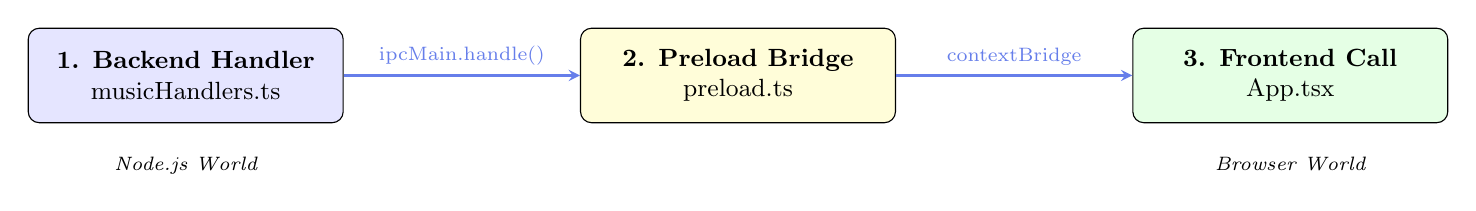
\begin{tikzpicture}[
    node distance=1.5cm,
    file/.style={draw, rounded corners, minimum width=4cm, minimum height=1.2cm, align=center, font=\small},
    code/.style={draw, rectangle, fill=gray!5, minimum width=5cm, align=left, font=\ttfamily\tiny},
    arrow/.style={->, thick, >=stealth, accentcolor}
]
    % Three layers
    \node[file, fill=blue!10] (backend) {\textbf{1. Backend Handler}\\musicHandlers.ts};
    \node[file, fill=yellow!15, right=3cm of backend] (preload) {\textbf{2. Preload Bridge}\\preload.ts};
    \node[file, fill=green!10, right=3cm of preload] (frontend) {\textbf{3. Frontend Call}\\App.tsx};
    
    % Arrows with method names
    \draw[arrow] (backend) -- node[above, font=\scriptsize] {ipcMain.handle()} (preload);
    \draw[arrow] (preload) -- node[above, font=\scriptsize] {contextBridge} (frontend);
    
    % Labels
    \node[below=0.3cm of backend, font=\scriptsize\itshape] {Node.js World};
    \node[below=0.3cm of frontend, font=\scriptsize\itshape] {Browser World};
\end{tikzpicture}
\caption{The Three-Layer IPC Pattern}
\label{fig:ipc_three_layer}
\end{figure}

\subsection{Step 1: Backend Handler (The Actual Work)}

This is where the real work happens. The handler has \textbf{full access} to Node.js APIs (file system, databases, network).

\begin{lstlisting}[language=TypeScript, title=electron/ipc/modules/musicHandlers.ts]
import { ipcMain } from 'electron';
import { scanMusicFiles } from '../../musicScanner';

export function registerMusicHandlers() {
  // Register a handler for 'scan-music-folder' channel
  ipcMain.handle('scan-music-folder', async (event, folderPath: string) => {
    try {
      // This code runs in Node.js - full file system access!
      const files = await scanMusicFiles(folderPath);
      return { success: true, data: files };
    } catch (error) {
      return { success: false, error: error.message };
    }
  });
}
\end{lstlisting}

\begin{infobox}
\textbf{Key Method:} \inlinecode{ipcMain.handle(channelName, handlerFunction)}

This registers a handler that the frontend can call. The handler receives any arguments passed from the frontend and can return a value (or Promise).
\end{infobox}

\subsection{Step 2: Preload Bridge (The Secure Gateway)}

The preload script runs in a \textbf{special context} --- it can access both Node.js and browser APIs, but it's isolated from both. Its job is to create a \textbf{safe, limited API} for the frontend.

\begin{lstlisting}[language=TypeScript, title=electron/preload.ts]
import { contextBridge, ipcRenderer } from 'electron';

// Expose a safe API to the renderer (frontend)
contextBridge.exposeInMainWorld('electronAPI', {
  // This is what the frontend will call
  scanMusicFolder: (folderPath: string) => {
    // Forward to the backend handler via IPC
    return ipcRenderer.invoke('scan-music-folder', folderPath);
  },
  
  // More functions can be added here...
  selectMusicFolder: () => ipcRenderer.invoke('select-music-folder'),
  getSettings: () => ipcRenderer.invoke('get-settings'),
});
\end{lstlisting}

\begin{warningbox}
\textbf{Key Method:} \inlinecode{contextBridge.exposeInMainWorld(apiName, apiObject)}

This is \textbf{THE} security mechanism. It creates a \inlinecode{window.electronAPI} object that the frontend can access, but with \textbf{only the functions you explicitly define}. The frontend cannot access \inlinecode{require()}, \inlinecode{fs}, or any other Node.js APIs.
\end{warningbox}

\subsection{Step 3: Frontend Call (React Component)}

The frontend calls the exposed API just like any async function. It has \textbf{no idea} that Node.js is involved --- it just sees a Promise-based API.

\begin{lstlisting}[language=TypeScript, title=src/App.tsx]
// The frontend calls window.electronAPI
const handleScanFolder = async () => {
  const folderPath = '/Users/music/library';
  
  // This looks like a normal async call!
  const result = await window.electronAPI.scanMusicFolder(folderPath);
  
  if (result.success) {
    setMusicFiles(result.data);  // Update React state
    console.log(`Found ${result.data.length} songs!`);
  } else {
    showError(result.error);
  }
};
\end{lstlisting}

\subsection{Complete Data Flow Visualization}

\begin{figure}[ht!]
\centering
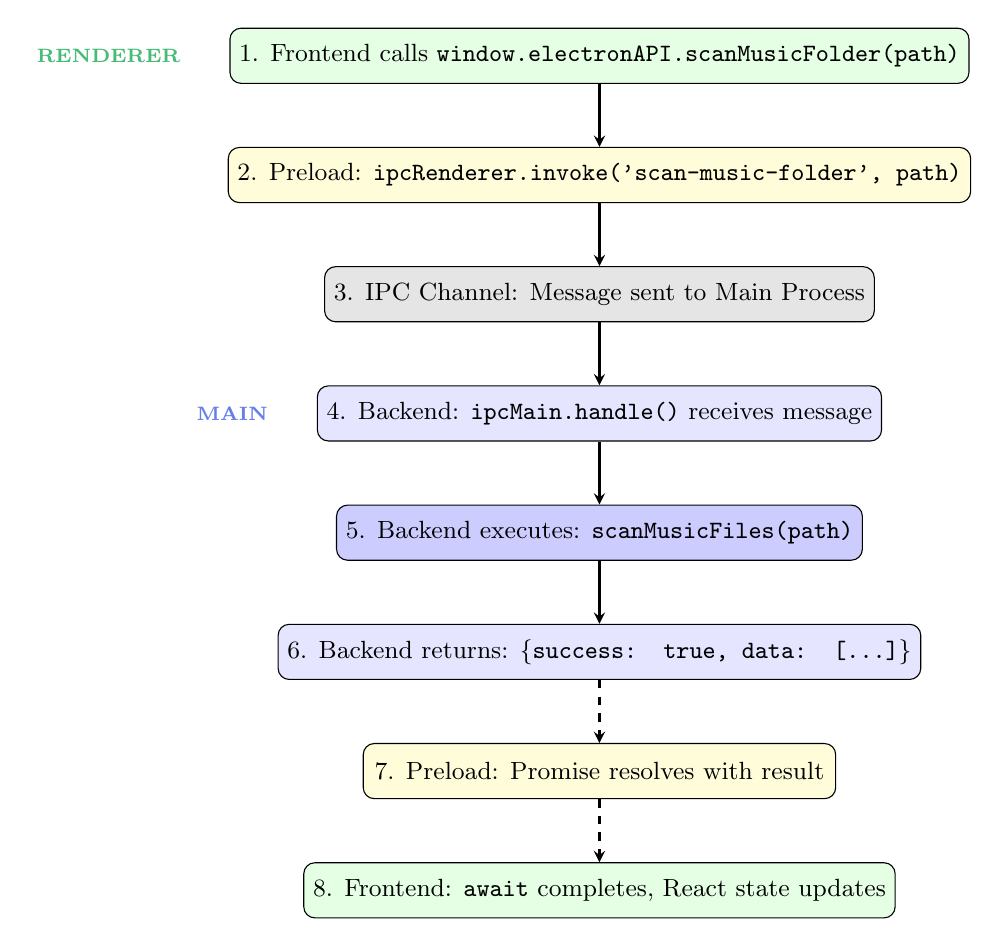
\begin{tikzpicture}[
    node distance=0.8cm,
    ipcstep/.style={draw, rounded corners, minimum width=6cm, minimum height=0.7cm, align=center, font=\small},
    code/.style={draw, rectangle, fill=gray!5, minimum width=6cm, align=left, font=\ttfamily\scriptsize},
    arrow/.style={->, thick, >=stealth}
]
    % Frontend
    \node[ipcstep, fill=green!10] (call) {1. Frontend calls \texttt{window.electronAPI.scanMusicFolder(path)}};
    
    % Preload
    \node[ipcstep, fill=yellow!15, below=of call] (preload) {2. Preload: \texttt{ipcRenderer.invoke('scan-music-folder', path)}};
    
    % IPC Channel
    \node[ipcstep, fill=gray!20, below=of preload] (ipc) {3. IPC Channel: Message sent to Main Process};
    
    % Backend
    \node[ipcstep, fill=blue!10, below=of ipc] (handler) {4. Backend: \texttt{ipcMain.handle()} receives message};
    
    % Work
    \node[ipcstep, fill=blue!20, below=of handler] (work) {5. Backend executes: \texttt{scanMusicFiles(path)}};
    
    % Response
    \node[ipcstep, fill=blue!10, below=of work] (response) {6. Backend returns: \texttt{\{success: true, data: [...]\}}};
    
    % Back up
    \node[ipcstep, fill=yellow!15, below=of response] (preload2) {7. Preload: Promise resolves with result};
    
    % Frontend receives
    \node[ipcstep, fill=green!10, below=of preload2] (receive) {8. Frontend: \texttt{await} completes, React state updates};
    
    % Arrows
    \draw[arrow] (call) -- (preload);
    \draw[arrow] (preload) -- (ipc);
    \draw[arrow] (ipc) -- (handler);
    \draw[arrow] (handler) -- (work);
    \draw[arrow] (work) -- (response);
    \draw[arrow, dashed] (response) -- (preload2);
    \draw[arrow, dashed] (preload2) -- (receive);
    
    % Labels
    \node[left=0.5cm of call, font=\scriptsize\bfseries, text=successcolor] {RENDERER};
    \node[left=0.5cm of handler, font=\scriptsize\bfseries, text=accentcolor] {MAIN};
\end{tikzpicture}
\caption{Complete IPC Round-Trip: Request and Response Flow}
\label{fig:ipc_roundtrip}
\end{figure}

\subsection{The Two IPC Methods}

Electron provides two ways to communicate:

\begin{table}[ht!]
\centering
\begin{tabular}{@{}p{3cm}p{4cm}p{6cm}@{}}
\toprule
\textbf{Method} & \textbf{Pattern} & \textbf{Use Case} \\
\midrule
\inlinecode{invoke/handle} & Request $\rightarrow$ Response & When you need a result back (scanning, API calls) \\
\inlinecode{send/on} & Fire \& Forget & When you don't need a response (window minimize) \\
\bottomrule
\end{tabular}
\caption{IPC Communication Methods}
\end{table}

\textbf{Example of send/on (fire \& forget):}

\begin{lstlisting}[language=TypeScript]
// Preload (no return value)
minimizeWindow: () => ipcRenderer.send('window-minimize'),

// Backend (uses 'on' instead of 'handle')
ipcMain.on('window-minimize', () => {
  mainWindow.minimize();  // No return value
});
\end{lstlisting}

\subsection{Why This Pattern Matters}

\begin{itemize}
    \item \textbf{Security}: The frontend \textbf{cannot} access \inlinecode{require()}, \inlinecode{fs}, or any Node.js API directly. It can only call the functions you explicitly expose.
    \item \textbf{Type Safety}: TypeScript interfaces in \filepath{src/types/electron.d.ts} define exactly what \inlinecode{window.electronAPI} contains.
    \item \textbf{Maintainability}: Each handler module (\filepath{musicHandlers.ts}, \filepath{playlistHandlers.ts}, etc.) is focused on one feature.
    \item \textbf{Testability}: Backend handlers can be unit tested independently of the UI.
\end{itemize}

\begin{tipbox}
\textbf{Summary}: To expose a backend function to the frontend:
\begin{enumerate}
    \item Create a handler with \inlinecode{ipcMain.handle('channel-name', fn)}
    \item Expose it in preload with \inlinecode{contextBridge.exposeInMainWorld()}
    \item Call it from React with \inlinecode{await window.electronAPI.yourFunction()}
\end{enumerate}
\end{tipbox}

%------------------------------------------------------------------------------
% OBJECT-ORIENTED PROGRAMMING SECTION
%------------------------------------------------------------------------------
\section{Object-Oriented Programming (OOP) Basics}

\begin{infobox}
\textbf{New to programming concepts?} This section explains the core ideas behind how modern code is organized. These concepts appear throughout this codebase and most professional software.
\end{infobox}

Object-Oriented Programming (OOP) is a way of organizing code around ``objects'' --- bundles of data and the functions that work with that data. Let's explore the key concepts with everyday analogies.

\subsection{Encapsulation: Hiding the Messy Details}

\begin{tipbox}
\textbf{Analogy: A Car Dashboard}

When you drive a car, you interact with a simple interface: steering wheel, gas pedal, brake. You don't need to understand the engine's internal combustion process --- that complexity is \textbf{hidden} from you.

\textbf{Encapsulation} means bundling data with the methods that operate on it, and hiding internal details from the outside world.
\end{tipbox}

\begin{figure}[ht!]
\centering
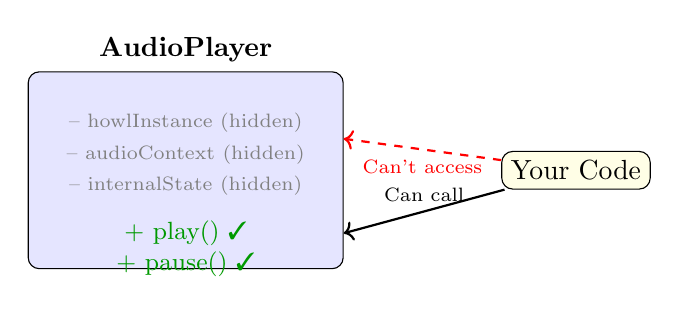
\begin{tikzpicture}[
    box/.style={draw, rounded corners, minimum width=4cm, minimum height=2.5cm, align=center},
    hidden/.style={font=\scriptsize, gray},
    public/.style={font=\small, black}
]
    % The object
    \node[box, fill=blue!10] (obj) at (0, 0) {};
    \node[above=0cm of obj, font=\bfseries] {AudioPlayer};
    
    % Hidden internals
    \node[hidden] at (0, 0.6) {-- howlInstance (hidden)};
    \node[hidden] at (0, 0.2) {-- audioContext (hidden)};
    \node[hidden] at (0, -0.2) {-- internalState (hidden)};
    
    % Public interface
    \node[public, green!60!black] at (0, -0.8) {+ play() \cmark};
    \node[public, green!60!black] at (0, -1.2) {+ pause() \cmark};
    
    % Outside world
    \node[draw, rounded corners, fill=yellow!10, right=2cm of obj] (user) {Your Code};
    
    \draw[->, thick] (user) -- node[above, font=\scriptsize] {Can call} (obj.east |- 0,-0.8);
    \draw[->, thick, red, dashed] (user) -- node[below, font=\scriptsize, red] {Can't access} (obj.east |- 0,0.4);
\end{tikzpicture}
\caption{Encapsulation: Public Interface vs Hidden Internals}
\label{fig:encapsulation}
\end{figure}

\textbf{In this codebase}: The \inlinecode{useAudioPlayer} hook exposes simple functions like \inlinecode{play()}, \inlinecode{pause()}, \inlinecode{next()}, but hides the complex Howler.js audio management internally.

\subsection{Abstraction: Simplifying Complex Things}

\begin{tipbox}
\textbf{Analogy: A TV Remote}

A remote control is an \textbf{abstraction} of the TV. Instead of understanding circuits and signals, you just press ``Volume Up.'' The remote \textbf{abstracts away} the complexity into simple buttons.

\textbf{Abstraction} means representing complex systems with simplified interfaces.
\end{tipbox}

\begin{lstlisting}[language=TypeScript, title=Abstraction Example]
// Complex reality: scanning involves fingerprinting, API calls, 
// rate limiting, caching, tag writing...

// Abstracted interface: one simple function
await window.electronAPI.scanSongs(selectedSongs);

// You don't need to know HOW it works internally
\end{lstlisting}

\textbf{In this codebase}: The \inlinecode{electronAPI} abstracts away all IPC complexity. React components just call simple functions without knowing about Electron's internal messaging.

\subsection{Interfaces: Contracts for Code}

\begin{tipbox}
\textbf{Analogy: A Job Description}

An interface is like a \textbf{job description}. It lists what abilities are required (``must be able to fly''), but doesn't specify HOW to do it. A bird and an airplane both satisfy the ``can fly'' requirement, but they implement it very differently.
\end{tipbox}

\begin{figure}[ht!]
\centering
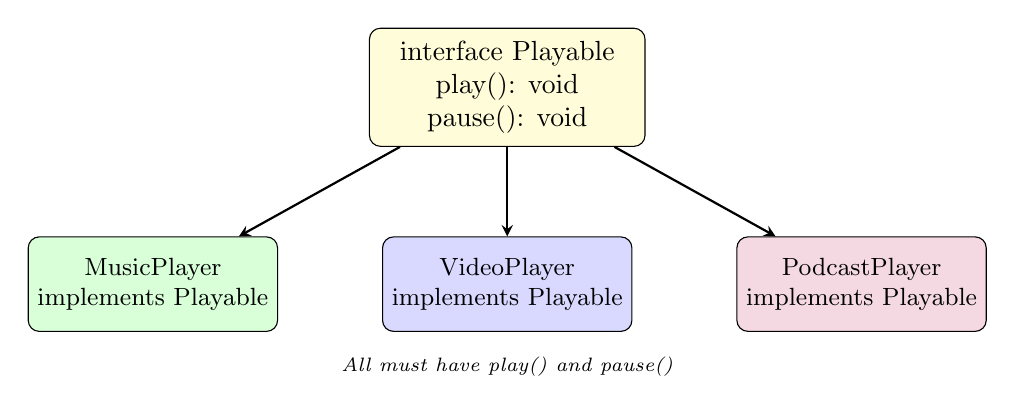
\begin{tikzpicture}[
    interface/.style={draw, rounded corners, minimum width=3.5cm, minimum height=1.5cm, align=center, fill=yellow!15},
    impl/.style={draw, rounded corners, minimum width=2.8cm, minimum height=1.2cm, align=center, font=\small},
    arrow/.style={->, thick, >=stealth}
]
    % Interface
    \node[interface] (iface) at (0, 2) {interface Playable\\play(): void\\pause(): void};
    
    % Implementations - spaced further apart
    \node[impl, fill=green!15] (music) at (-4.5, -0.5) {MusicPlayer\\implements Playable};
    \node[impl, fill=blue!15] (video) at (0, -0.5) {VideoPlayer\\implements Playable};
    \node[impl, fill=purple!15] (podcast) at (4.5, -0.5) {PodcastPlayer\\implements Playable};
    
    \draw[arrow] (iface) -- (music);
    \draw[arrow] (iface) -- (video);
    \draw[arrow] (iface) -- (podcast);
    
    \node[below=0.2cm of video, font=\scriptsize\itshape] {All must have play() and pause()};
\end{tikzpicture}
\caption{Interface: One Contract, Multiple Implementations}
\label{fig:interface_oop}
\end{figure}

\begin{lstlisting}[language=TypeScript, title=Interface in TypeScript]
// The contract
interface MusicFile {
  path: string;
  title: string;
  play(): void;
}

// Any object that has these properties/methods 
// satisfies the MusicFile interface
\end{lstlisting}

\textbf{In this codebase}: The \inlinecode{MusicFile} interface ensures every song object has the same properties, making the code predictable and type-safe.

\subsection{Inheritance: Building on What Exists}

\begin{tipbox}
\textbf{Analogy: Family Traits}

Children inherit traits from their parents --- eye color, height, etc. They get the parent's features ``for free'' and can add their own unique traits.

\textbf{Inheritance} lets you create new classes based on existing ones, reusing code without rewriting it.
\end{tipbox}

\begin{figure}[ht!]
\centering
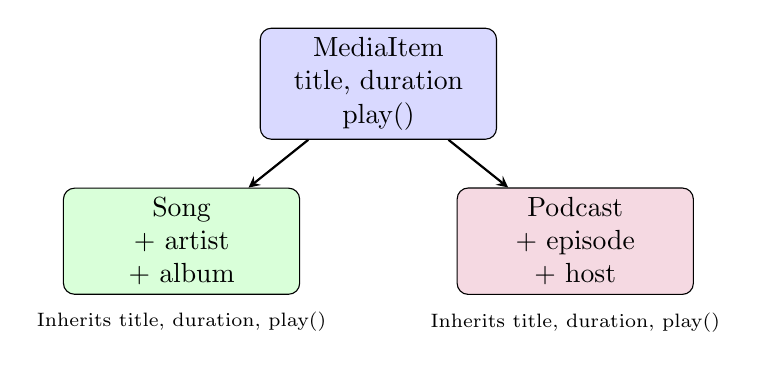
\begin{tikzpicture}[
    class/.style={draw, rounded corners, minimum width=3cm, minimum height=1.2cm, align=center},
    arrow/.style={->, thick, >=stealth}
]
    % Parent
    \node[class, fill=blue!15] (parent) at (0, 2) {MediaItem\\title, duration\\play()};
    
    % Children
    \node[class, fill=green!15] (song) at (-2.5, 0) {Song\\+ artist\\+ album};
    \node[class, fill=purple!15] (podcast) at (2.5, 0) {Podcast\\+ episode\\+ host};
    
    \draw[arrow] (parent) -- (song);
    \draw[arrow] (parent) -- (podcast);
    
    \node[below=0.1cm of song, font=\scriptsize] {Inherits title, duration, play()};
    \node[below=0.1cm of podcast, font=\scriptsize] {Inherits title, duration, play()};
\end{tikzpicture}
\caption{Inheritance: Children Extend Parents}
\label{fig:inheritance}
\end{figure}

\begin{lstlisting}[language=TypeScript, title=Inheritance Example]
class MediaItem {
  title: string;
  duration: number;
  play() { /* base implementation */ }
}

class Song extends MediaItem {
  artist: string;  // Song-specific
  album: string;   // Song-specific
  // Automatically has title, duration, play() from parent
}
\end{lstlisting}

\subsection{Polymorphism: Same Action, Different Behaviors}

\begin{tipbox}
\textbf{Analogy: The ``Speak'' Command}

If you tell a dog to ``speak,'' it barks. If you tell a cat to ``speak,'' it meows. Same command, different behavior based on who's receiving it.

\textbf{Polymorphism} means the same method name can behave differently depending on the object.
\end{tipbox}

\begin{figure}[ht!]
\centering
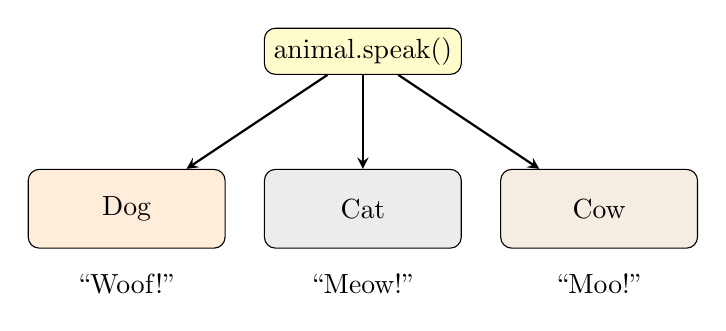
\begin{tikzpicture}[
    animal/.style={draw, rounded corners, minimum width=2.5cm, minimum height=1cm, align=center},
    arrow/.style={->, thick, >=stealth}
]
    % Command
    \node[draw, fill=yellow!20, rounded corners] (cmd) at (0, 2) {animal.speak()};
    
    % Animals
    \node[animal, fill=orange!15] (dog) at (-3, 0) {Dog};
    \node[animal, fill=gray!15] (cat) at (0, 0) {Cat};
    \node[animal, fill=brown!15] (cow) at (3, 0) {Cow};
    
    \draw[arrow] (cmd) -- (dog);
    \draw[arrow] (cmd) -- (cat);
    \draw[arrow] (cmd) -- (cow);
    
    \node[below=0.2cm of dog] {``Woof!''};
    \node[below=0.2cm of cat] {``Meow!''};
    \node[below=0.2cm of cow] {``Moo!''};
\end{tikzpicture}
\caption{Polymorphism: Same Method, Different Behaviors}
\label{fig:polymorphism}
\end{figure}

\textbf{In this codebase}: The notification system uses polymorphism --- calling \inlinecode{show()} on different notification types (success, error, warning) produces different colored toasts.

\subsection{OOP Summary Table}

\begin{table}[ht!]
\centering
\begin{tabular}{@{}p{3cm}p{4cm}p{6.5cm}@{}}
\toprule
\textbf{Concept} & \textbf{Analogy} & \textbf{What It Does} \\
\midrule
Encapsulation & Car dashboard & Hides complexity, exposes simple controls \\
Abstraction & TV remote & Simplifies complex systems into easy actions \\
Interface & Job description & Defines requirements without implementation \\
Inheritance & Family traits & Child classes get parent features for free \\
Polymorphism & ``Speak'' command & Same method, different behaviors per object \\
\bottomrule
\end{tabular}
\caption{OOP Concepts at a Glance}
\end{table}

\begin{tipbox}
\textbf{Why OOP Matters}: These concepts make large codebases manageable. Instead of one giant file with thousands of lines, code is organized into logical pieces that are easier to understand, test, and modify independently.
\end{tipbox}

\subsection{Real OOP Examples in This App}

Here are actual examples of OOP patterns used in this codebase:

\subsubsection{Class with Encapsulation: ParallelMetadataScanner}

The \filepath{parallelMetadataScanner.ts} file contains a class that demonstrates encapsulation perfectly:

\begin{lstlisting}[language=TypeScript, title=electron/parallelMetadataScanner.ts (simplified)]
export class ParallelMetadataScanner {
    // PRIVATE: Hidden from outside code
    private numWorkers: number
    private queue: ScanJob[] = []
    private completedCount: number = 0
    private isScanning: boolean = false
    
    // PUBLIC: The only way to interact with this class
    constructor(concurrency?: number) {
        const cpuCount = os.cpus().length;
        // Leave 1 core for UI, min 2, max 16
        this.numWorkers = concurrency ?? Math.max(2, Math.min(cpuCount - 1, 16));
    }
    
    setProgressCallback(callback: ProgressCallback): void {
        this.onProgress = callback
    }
    
    async scanDirectory(path: string): Promise<MusicFile[]> {
        // Complex logic hidden here...
    }
}
\end{lstlisting}

\begin{itemize}
    \item \textbf{Encapsulation}: The \inlinecode{private} keyword hides internal state (\inlinecode{queue}, \inlinecode{completedCount}, \inlinecode{isScanning}) from outside code
    \item \textbf{Abstraction}: You just call \inlinecode{scanDirectory(path)} --- the complex parallel worker logic is hidden
    \item You don't need to know that internally it creates multiple workers, manages a job queue, and tracks progress
\end{itemize}

\subsubsection{Class with Worker Pool Pattern: FingerprintWorkerPool}

The \filepath{fingerprintWorkerPool.ts} demonstrates a more complex class:

\begin{lstlisting}[language=TypeScript, title=electron/fingerprintWorkerPool.ts (simplified)]
class FingerprintWorkerPool {
    private workerCount: number
    private slots: WorkerSlot[]    // Each slot is one worker
    private queue: QueuedJob[] = []
    private isProcessing: boolean = false
    
    // Private helper - outside code can't call this
    private getAvailableSlot(): WorkerSlot | null {
        return this.slots.find(slot => !slot.busy) || null
    }
    
    // Private - manages job processing internally
    private async processJob(slot: WorkerSlot, job: QueuedJob) {
        // Complex processing logic...
    }
    
    // PUBLIC: Simple interface for users
    async processAll(filePaths: string[]): Promise<FingerprintJobResult[]> {
        // Internally manages parallel workers, but user just awaits results
    }
    
    getStatus(): PoolStatus {
        return { workerCount: this.workerCount, ... }
    }
}
\end{lstlisting}

\begin{figure}[ht!]
\centering
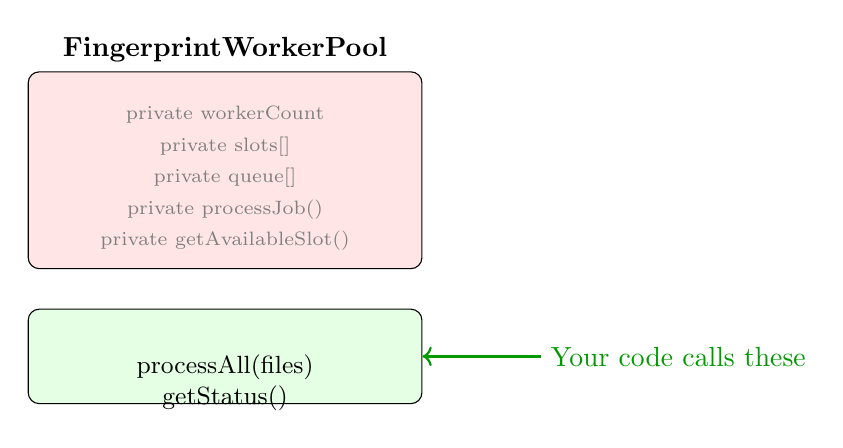
\begin{tikzpicture}[
    box/.style={draw, rounded corners, minimum width=5cm, align=center, font=\small},
    hidden/.style={fill=red!10},
    public/.style={fill=green!10}
]
    \node[box, hidden, minimum height=2.5cm] (hidden) at (0, 0) {};
    \node[above=0cm of hidden, font=\bfseries] {FingerprintWorkerPool};
    \node[font=\scriptsize, gray] at (0, 0.7) {private workerCount};
    \node[font=\scriptsize, gray] at (0, 0.3) {private slots[]};
    \node[font=\scriptsize, gray] at (0, -0.1) {private queue[]};
    \node[font=\scriptsize, gray] at (0, -0.5) {private processJob()};
    \node[font=\scriptsize, gray] at (0, -0.9) {private getAvailableSlot()};
    
    \node[box, public, minimum height=1.2cm, below=0.5cm of hidden] (public) {};
    \node[font=\small] at (0, -2.5) {processAll(files)};
    \node[font=\small] at (0, -2.9) {getStatus()};
    
    \draw[<-, thick, green!60!black] (public.east) -- ++(1.5, 0) node[right] {Your code calls these};
\end{tikzpicture}
\caption{Real Encapsulation: FingerprintWorkerPool}
\label{fig:real_encapsulation}
\end{figure}

\subsubsection{Interfaces in the Codebase}

This app uses many interfaces. Here are some real ones:

\begin{lstlisting}[language=TypeScript, title=Real Interfaces from the Codebase]
// From electron/musicScanner.ts
export interface MusicFile {
    path: string
    name: string
    extension: string
    size: number
    dateAdded: number
    metadata?: {
        title?: string
        artist?: string
        album?: string
        duration?: number
        albumArt?: string
    }
}

// From electron/settings.ts
export interface AppSettings {
    musicFolderPath: string | null
    scanSubfolders: boolean
    workerCount: number
    visualizerType: 'bars' | 'wave' | 'circular'
}

// From electron/youtubeDownloader.ts
export interface DownloadProgress {
    percent: number
    downloadedBytes: number
    totalBytes: number
    speed: string
}
\end{lstlisting}

These interfaces ensure:
\begin{itemize}
    \item Every \inlinecode{MusicFile} has the same shape throughout the app
    \item Settings always have the expected properties
    \item Download progress reports are consistent
\end{itemize}

\subsubsection{Singleton Pattern}

Both worker pool classes use the \textbf{Singleton Pattern} --- ensuring only one instance exists:

\begin{lstlisting}[language=TypeScript, title=Singleton Pattern]
// Only ONE instance of the scanner exists
let scannerInstance: ParallelMetadataScanner | null = null

export function getParallelScanner(): ParallelMetadataScanner {
    if (!scannerInstance) {
        scannerInstance = new ParallelMetadataScanner()
    }
    return scannerInstance  // Always returns the SAME instance
}
\end{lstlisting}

\begin{tipbox}
\textbf{Why Singleton?} We only want one worker pool managing scans. If we created multiple pools, they'd compete for CPU resources and create chaos. The singleton ensures controlled, coordinated processing.
\end{tipbox}

\subsubsection{OOP in React: Custom Hooks}

While React uses functions, not classes, the \textbf{spirit of OOP} appears in custom hooks:

\begin{lstlisting}[language=TypeScript, title=src/hooks/useAudioPlayer.ts (concept)]
function useAudioPlayer() {
    // "Private" state - not directly accessible
    const [currentSong, setCurrentSong] = useState(null)
    const [isPlaying, setIsPlaying] = useState(false)
    const howlRef = useRef(null)  // Internal Howler instance
    
    // "Public" methods returned to caller
    const play = () => { ... }
    const pause = () => { ... }
    const next = () => { ... }
    const setVolume = (v) => { ... }
    
    // Return only what components need
    return { currentSong, isPlaying, play, pause, next, setVolume }
}
\end{lstlisting}

This is \textbf{encapsulation} in functional form:
\begin{itemize}
    \item Internal state (\inlinecode{howlRef}) is hidden
    \item Components only see simple functions (\inlinecode{play}, \inlinecode{pause})
    \item The complex Howler.js audio management is abstracted away
\end{itemize}

%------------------------------------------------------------------------------
% TYPESCRIPT SECTION
%------------------------------------------------------------------------------
\section{Understanding TypeScript}

This project is written entirely in \techterm{TypeScript} instead of plain JavaScript. This section explains what TypeScript is, why we use it, and where you'll see it throughout the codebase.

\subsection{TypeScript 101: The Absolute Basics}

\begin{infobox}
\textbf{Never used TypeScript before?} This section is for you! We'll explain the core concept with simple analogies before showing any code.
\end{infobox}

\subsubsection{The Problem TypeScript Solves}

Imagine you're ordering food at a restaurant. You tell the waiter:

\begin{itemize}
    \item ``I'd like the number 7'' --- The waiter knows exactly what to bring
    \item ``I'd like something'' --- The waiter has no idea what you want
\end{itemize}

JavaScript is like the second situation. Functions accept ``something'' without knowing what that something should be. This causes bugs that only appear when the program runs.

\textbf{TypeScript} is like the first situation. Every value has a \textbf{label} saying what it is, so mistakes are caught immediately.

\subsubsection{A Simple Analogy: Labeled Boxes}

Think of variables as boxes that hold values:

\begin{table}[ht!]
\centering
\begin{tabular}{@{}ccc@{}}
\toprule
\textbf{JavaScript} & \textbf{TypeScript} & \textbf{What's Inside} \\
\midrule
\fbox{???} & \fbox{string} & ``Hello World'' \\
\fbox{???} & \fbox{number} & 42 \\
\fbox{???} & \fbox{boolean} & true \\
\fbox{???} & \fbox{MusicFile} & \{title, artist, path...\} \\
\bottomrule
\end{tabular}
\end{table}

\begin{figure}[ht!]
\centering
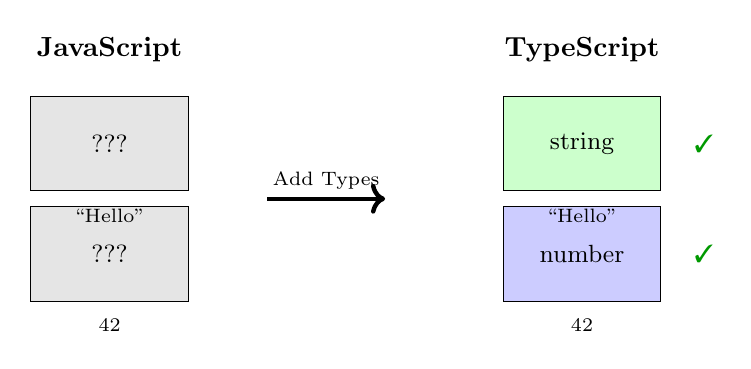
\begin{tikzpicture}[
    box/.style={draw, minimum width=2cm, minimum height=1.2cm, align=center, font=\small},
    label/.style={font=\scriptsize\bfseries, fill=white}
]
    % JavaScript side
    \node[font=\bfseries] at (-2, 2) {JavaScript};
    \node[box, fill=gray!20] (js1) at (-2, 0.8) {???};
    \node[box, fill=gray!20] (js2) at (-2, -0.6) {???};
    \node[below=0.1cm of js1, font=\scriptsize] {``Hello''};
    \node[below=0.1cm of js2, font=\scriptsize] {42};
    
    % Arrow
    \draw[->, ultra thick] (0, 0.1) -- (1.5, 0.1);
    \node[above] at (0.75, 0.1) {\scriptsize Add Types};
    
    % TypeScript side
    \node[font=\bfseries] at (4, 2) {TypeScript};
    \node[box, fill=green!20] (ts1) at (4, 0.8) {string};
    \node[box, fill=blue!20] (ts2) at (4, -0.6) {number};
    \node[below=0.1cm of ts1, font=\scriptsize] {``Hello''};
    \node[below=0.1cm of ts2, font=\scriptsize] {42};
    
    % Checkmarks
    \node[right=0.3cm of ts1, font=\small, green!60!black] {\cmark};
    \node[right=0.3cm of ts2, font=\small, green!60!black] {\cmark};
\end{tikzpicture}
\caption{JavaScript vs TypeScript: Unlabeled vs Labeled Boxes}
\label{fig:labeled_boxes}
\end{figure}

In JavaScript, boxes have no labels --- you don't know what's inside until you open them. In TypeScript, every box is \textbf{labeled} with its contents. If you try to put a number in a string box, TypeScript stops you.

\subsubsection{The Core Syntax: One Thing to Remember}

The \textbf{colon (:)} means ``is a'':

\begin{verbatim}
  name: string       means    name IS A string
  age: number        means    age IS A number
  song: MusicFile    means    song IS A MusicFile
\end{verbatim}

That's it! When you see a colon followed by a word, it's just saying ``this variable/parameter is a [type]''.

\subsubsection{Reading TypeScript Code}

Here's how to read TypeScript if you've never seen it:

\begin{lstlisting}[language=TypeScript, title=Reading TypeScript Out Loud]
// Read this as: 
// "name is a string, returns a string"
function greet(name: string): string {
  return "Hello, " + name;
}

// Read this as:
// "song is a MusicFile"
const song: MusicFile = getMusicFile();

// Read this as:
// "items is an array of strings"
const items: string[] = ["rock", "pop", "jazz"];
\end{lstlisting}

\subsubsection{Why Bother?}

\begin{table}[ht!]
\centering
\begin{tabular}{@{}p{6cm}p{7.5cm}@{}}
\toprule
\textbf{Without Types (JavaScript)} & \textbf{With Types (TypeScript)} \\
\midrule
Bug appears when user clicks button & Bug appears while you're writing code \\
Error message is cryptic: ``undefined is not a function'' & Error message is clear: ``Property 'title' does not exist'' \\
You must remember what every function expects & Editor tells you what every function expects \\
Refactoring is scary & Refactoring is safe --- compiler catches broken code \\
\bottomrule
\end{tabular}
\end{table}

\begin{tipbox}
\textbf{Bottom Line}: TypeScript is just JavaScript with labels. The labels help catch bugs before your program runs, and help your editor give you better autocomplete.
\end{tipbox}

\subsection{What is TypeScript? (Technical Details)}

\techterm{TypeScript} is JavaScript with \textbf{type annotations}. It's a language created by Microsoft that compiles down to regular JavaScript.

\begin{lstlisting}[language=TypeScript, title=Plain JavaScript (no types)]
function greet(name) {
  return "Hello, " + name;
}
greet(42);  // No error - but this is probably a bug!
\end{lstlisting}

\begin{lstlisting}[language=TypeScript, title=TypeScript (with types)]
function greet(name: string): string {
  return "Hello, " + name;
}
greet(42);  // ERROR: Argument of type 'number' is not 
            // assignable to parameter of type 'string'
\end{lstlisting}

\begin{infobox}
\textbf{Key Point}: TypeScript catches bugs \textbf{before} you run your code. The compiler tells you about type mismatches, missing properties, and other issues at build time rather than at runtime.
\end{infobox}

\subsection{Why TypeScript for This Project?}

We chose TypeScript for several critical reasons:

\begin{enumerate}
    \item \textbf{IPC Type Safety} --- The communication between Main and Renderer processes involves complex data structures. TypeScript ensures both sides agree on the shape of data.
    
    \item \textbf{Large Codebase} --- With 50+ files across frontend and backend, TypeScript makes refactoring safe. Change a function signature and the compiler tells you every place that needs updating.
    
    \item \textbf{IDE Support} --- VS Code provides autocomplete, hover documentation, and inline error checking because it understands TypeScript types.
    
    \item \textbf{Self-Documenting Code} --- Types serve as documentation. When you see \inlinecode{file: MusicFile}, you immediately know what properties are available.
\end{enumerate}

\subsection{Where TypeScript is Used}

TypeScript is used in \textbf{every part} of this application:

\begin{figure}[ht!]
\centering
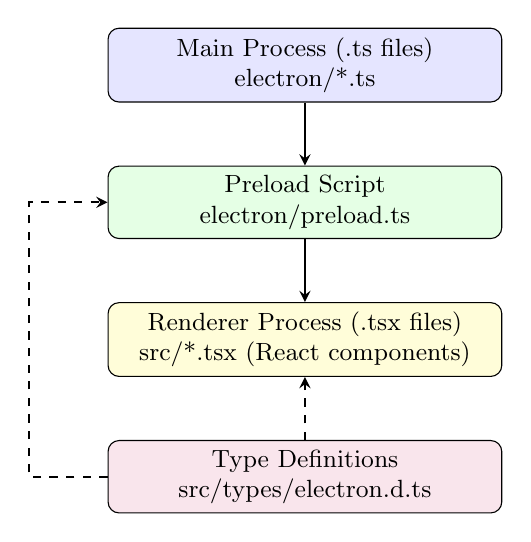
\begin{tikzpicture}[
    node distance=0.8cm,
    box/.style={draw, rounded corners, minimum width=5cm, minimum height=0.7cm, align=center, font=\small},
    arrow/.style={->, thick, >=stealth}
]
    \node[box, fill=blue!10] (main) {Main Process (.ts files)\\electron/*.ts};
    \node[box, fill=green!10, below=of main] (preload) {Preload Script\\electron/preload.ts};
    \node[box, fill=yellow!15, below=of preload] (renderer) {Renderer Process (.tsx files)\\src/*.tsx (React components)};
    \node[box, fill=purple!10, below=of renderer] (types) {Type Definitions\\src/types/electron.d.ts};
    
    \draw[arrow] (main) -- (preload);
    \draw[arrow] (preload) -- (renderer);
    \draw[arrow, dashed] (types) -- (renderer);
    \draw[arrow, dashed] (types.west) -- ++(-1,0) |- (preload.west);
\end{tikzpicture}
\caption{TypeScript Usage Across the Application}
\label{fig:typescript_usage}
\end{figure}

\subsection{File Extensions Explained}

\begin{table}[ht!]
\centering
\begin{tabular}{@{}p{2.5cm}p{4cm}p{7cm}@{}}
\toprule
\textbf{Extension} & \textbf{What it is} & \textbf{Where used} \\
\midrule
\inlinecode{.ts} & Pure TypeScript & Backend files in \filepath{electron/} \\
\inlinecode{.tsx} & TypeScript + JSX & React components in \filepath{src/} \\
\inlinecode{.d.ts} & Type declarations only & \filepath{src/types/electron.d.ts} (IPC types) \\
\bottomrule
\end{tabular}
\caption{TypeScript File Extensions}
\end{table}

\subsection{Practical Example: MusicFile Interface}

Here's a real example from our codebase. The \inlinecode{MusicFile} interface defines the shape of music file data:

\begin{lstlisting}[language=TypeScript, title=electron/musicScanner.ts]
export interface MusicFile {
  path: string;
  title: string;
  artist: string;
  album: string;
  duration: number;        // in seconds
  albumArt: string | null; // base64 or null
  year?: number;           // optional
}
\end{lstlisting}

Now anywhere in the app, when you have a variable of type \inlinecode{MusicFile}:

\begin{lstlisting}[language=TypeScript, title=Benefits in React Component]
function SongItem({ song }: { song: MusicFile }) {
  // TypeScript knows ALL these properties exist:
  console.log(song.path);     // OK
  console.log(song.title);    // OK
  console.log(song.artist);   // OK
  console.log(song.albumArt); // OK (string | null)
  console.log(song.year);     // OK (number | undefined)
  
  console.log(song.genre);    // ERROR: Property 'genre' 
                              // does not exist on type 'MusicFile'
}
\end{lstlisting}

\subsection{The electron.d.ts File}

One of the most important TypeScript files is \filepath{src/types/electron.d.ts}. This file defines ALL the functions available on \inlinecode{window.electronAPI}:

\begin{lstlisting}[language=TypeScript, title=src/types/electron.d.ts (simplified)]
interface ElectronAPI {
  // Music scanning
  scanMusicFolder: (path: string) => Promise<MusicFile[]>;
  selectMusicFolder: () => Promise<string | null>;
  
  // YouTube downloads
  downloadYouTube: (url: string) => Promise<DownloadResult>;
  onDownloadProgress: (callback: (progress: number) => void) => void;
  
  // Settings
  getSettings: () => Promise<AppSettings>;
  saveSettings: (settings: AppSettings) => Promise<void>;
  
  // ... 50+ more functions
}

declare global {
  interface Window {
    electronAPI: ElectronAPI;
  }
}
\end{lstlisting}

\begin{warningbox}
\textbf{Important}: When you add a new IPC channel in \filepath{preload.ts}, you \textbf{must} also update \filepath{electron.d.ts} with the matching type definition. Otherwise, TypeScript will show an error when you try to call the function from React.
\end{warningbox}

\subsection{TypeScript Compilation}

TypeScript files are \textbf{not} run directly. They are compiled to JavaScript:

\begin{figure}[ht!]
\centering
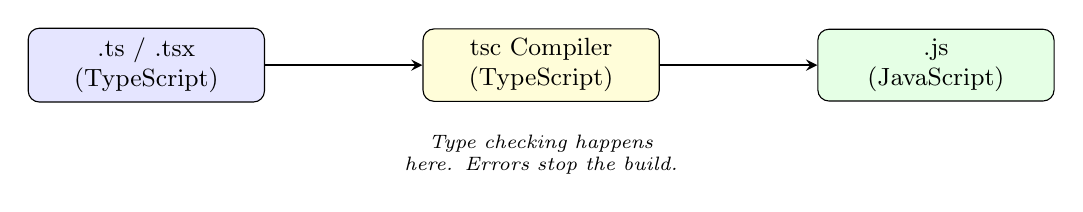
\begin{tikzpicture}[
    node distance=1.5cm,
    box/.style={draw, rounded corners, minimum width=3cm, minimum height=0.8cm, align=center, font=\small},
    arrow/.style={->, thick, >=stealth}
]
    \node[box, fill=blue!10] (ts) {.ts / .tsx\\(TypeScript)};
    \node[box, fill=yellow!15, right=2cm of ts] (tsc) {tsc Compiler\\(TypeScript)};
    \node[box, fill=green!10, right=2cm of tsc] (js) {.js\\(JavaScript)};
    
    \draw[arrow] (ts) -- (tsc);
    \draw[arrow] (tsc) -- (js);
    
    \node[below=0.3cm of tsc, font=\scriptsize\itshape, text width=4cm, align=center] {Type checking happens here. Errors stop the build.};
\end{tikzpicture}
\caption{TypeScript Compilation Process}
\label{fig:ts_compile}
\end{figure}

When you run \inlinecode{npm run dev} or \inlinecode{npm run build}:

\begin{enumerate}
    \item TypeScript compiler checks all \inlinecode{.ts} and \inlinecode{.tsx} files for errors
    \item If no errors, it generates \inlinecode{.js} files
    \item Vite bundles the JavaScript for the browser
    \item Electron runs the compiled JavaScript
\end{enumerate}

\subsection{Quick TypeScript Syntax Reference}

\begin{table}[ht!]
\centering
\begin{tabular}{@{}p{5cm}p{8.5cm}@{}}
\toprule
\textbf{TypeScript Syntax} & \textbf{Meaning} \\
\midrule
\inlinecode{name: string} & Variable must be a string \\
\inlinecode{count: number} & Variable must be a number \\
\inlinecode{isActive: boolean} & Variable must be true/false \\
\inlinecode{items: string[]} & Array of strings \\
\inlinecode{file: MusicFile} & Variable must match MusicFile interface \\
\inlinecode{data: string | null} & String OR null (union type) \\
\inlinecode{year?: number} & Optional property (may be undefined) \\
\inlinecode{Promise<MusicFile[]>} & Async function returning array of MusicFile \\
\inlinecode{() => void} & Function that takes nothing, returns nothing \\
\bottomrule
\end{tabular}
\caption{Common TypeScript Syntax Patterns}
\end{table}

\subsection{How Types Are Defined}

There are two main ways to define custom types in TypeScript:

\subsubsection{1. Using \texttt{interface} (Preferred for Objects)}

\begin{tipbox}
\textbf{Analogy: A Blueprint}

An \inlinecode{interface} is like a \textbf{blueprint for a house}. It says: ``Every house must have a door, windows, and a roof.'' You can't build a house without these parts. Similarly, a \inlinecode{MusicFile} interface says: ``Every music file must have a path, title, artist...'' and you can't create one without those properties.
\end{tipbox}

\begin{figure}[ht!]
\centering
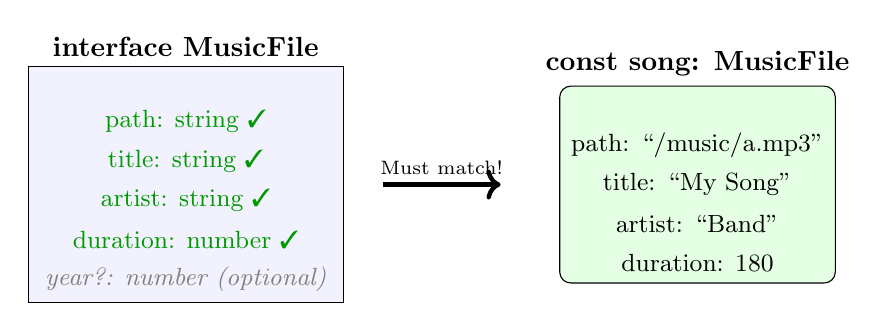
\begin{tikzpicture}[
    blueprint/.style={draw, minimum width=4cm, minimum height=3cm, align=left, font=\small, fill=blue!5},
    prop/.style={font=\small},
    required/.style={font=\small, green!60!black},
    optional/.style={font=\small\itshape, gray}
]
    % Blueprint box
    \node[blueprint] (bp) at (0, 0) {};
    \node[above=0cm of bp, font=\bfseries] {interface MusicFile};
    
    % Properties inside
    \node[required] at (0, 0.8) {path: string \cmark};
    \node[required] at (0, 0.3) {title: string \cmark};
    \node[required] at (0, -0.2) {artist: string \cmark};
    \node[required] at (0, -0.7) {duration: number \cmark};
    \node[optional] at (0, -1.2) {year?: number (optional)};
    
    % Arrow to object
    \draw[->, ultra thick] (2.5, 0) -- (4, 0);
    \node[above] at (3.25, 0) {\scriptsize Must match!};
    
    % Actual object
    \node[draw, minimum width=3.5cm, minimum height=2.5cm, align=left, fill=green!10, rounded corners] (obj) at (6.5, 0) {};
    \node[above=0cm of obj, font=\bfseries] {const song: MusicFile};
    \node[font=\small] at (6.5, 0.5) {path: ``/music/a.mp3''};
    \node[font=\small] at (6.5, 0) {title: ``My Song''};
    \node[font=\small] at (6.5, -0.5) {artist: ``Band''};
    \node[font=\small] at (6.5, -1) {duration: 180};
\end{tikzpicture}
\caption{Interface as a Blueprint for Objects}
\label{fig:interface_blueprint}
\end{figure}

An \inlinecode{interface} defines the shape of an object --- what properties it has and their types:

\begin{lstlisting}[language=TypeScript, title=Defining an Interface]
// Define the type
interface MusicFile {
  path: string;           // Required: must be a string
  title: string;          // Required: must be a string
  artist: string;         // Required: must be a string
  duration: number;       // Required: must be a number
  albumArt: string | null; // Required: string OR null
  year?: number;          // Optional: may not exist
}

// Now use it - TypeScript enforces the shape
const song: MusicFile = {
  path: "/music/song.mp3",
  title: "My Song",
  artist: "Artist Name",
  duration: 180,
  albumArt: null
  // year is optional, so we can omit it
};
\end{lstlisting}

\subsubsection{2. Using \texttt{type} (For Unions, Aliases)}

\begin{tipbox}
\textbf{Analogy: Nicknames and Multiple Choice}

A \inlinecode{type} is like giving something a \textbf{nickname}. Instead of saying ``text made of characters'' every time, you just say ``string.'' 

A \textbf{union type} is like a multiple-choice question where you can only pick ONE answer. \inlinecode{'unscanned' | 'scanned-tagged'} means: ``Pick one: unscanned OR scanned-tagged. Nothing else is allowed.''
\end{tipbox}

A \inlinecode{type} alias can represent simple values, unions, or complex types:

\begin{lstlisting}[language=TypeScript, title=Type Aliases]
// Simple alias
type FilePath = string;

// Union type - can be ONE of these values
type ScanStatus = 'unscanned' | 'scanned-tagged' | 'scanned-no-match';

// Union of different types
type ApiResult = MusicFile[] | null | Error;

// Usage
let status: ScanStatus = 'unscanned';    // OK
status = 'invalid';  // ERROR: not in the union
\end{lstlisting}

\subsection{How Functions Define Return Types}

\begin{tipbox}
\textbf{Analogy: A Vending Machine}

A function's return type is like the \textbf{label on a vending machine slot}. If the slot says ``Chips,'' you expect to get chips --- not soda. If a function says \inlinecode{: string}, it \textbf{must} give you a string. The compiler is like a quality control inspector making sure every machine delivers what it promises.
\end{tipbox}

\begin{figure}[ht!]
\centering
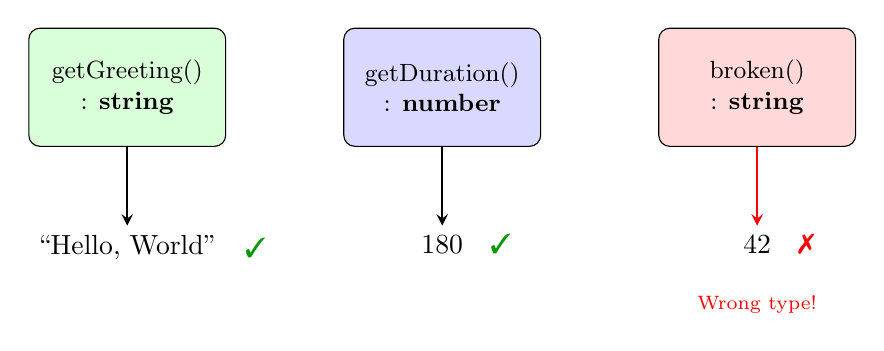
\begin{tikzpicture}[
    slot/.style={draw, minimum width=2.5cm, minimum height=1.5cm, align=center, font=\small, rounded corners},
    arrow/.style={->, thick, >=stealth}
]
    % Vending machine slots
    \node[slot, fill=green!15] (slot1) at (0, 0) {getGreeting()\\: \textbf{string}};
    \node[slot, fill=blue!15] (slot2) at (4, 0) {getDuration()\\: \textbf{number}};
    
    % Outputs
    \node[below=1cm of slot1] (out1) {``Hello, World''};
    \node[below=1cm of slot2] (out2) {180};
    
    \draw[arrow] (slot1) -- (out1);
    \draw[arrow] (slot2) -- (out2);
    
    % Checkmarks
    \node[right=0.1cm of out1, green!60!black] {\cmark};
    \node[right=0.1cm of out2, green!60!black] {\cmark};
    
    % Wrong example
    \node[slot, fill=red!15] (slot3) at (8, 0) {broken()\\: \textbf{string}};
    \node[below=1cm of slot3] (out3) {42};
    \draw[arrow, red] (slot3) -- (out3);
    \node[right=0.1cm of out3, red] {\xmark};
    \node[below=0.3cm of out3, font=\scriptsize, red] {Wrong type!};
\end{tikzpicture}
\caption{Functions Must Return What Their Type Promises}
\label{fig:vending_machine}
\end{figure}

Every function can specify what type of value it returns. The compiler \textbf{enforces} that the function actually returns that type.

\begin{lstlisting}[language=TypeScript, title=Function Return Types]
// The `: string` after () means this function MUST return a string
function getGreeting(name: string): string {
  return "Hello, " + name;  // OK - returns string
}

// The `: number` means MUST return a number
function calculateDuration(seconds: number): number {
  return seconds / 60;  // OK - returns number
}

// What if you return the wrong type?
function brokenExample(): string {
  return 42;  // ERROR: Type 'number' is not assignable to type 'string'
}
\end{lstlisting}

\subsection{Async Functions and Promise Types}

\begin{tipbox}
\textbf{Analogy: A Restaurant Ticket}

A \inlinecode{Promise} is like the \textbf{numbered ticket you get at a restaurant}. You don't get your food immediately --- you get a ticket that \textbf{promises} food later. \inlinecode{Promise<MusicFile[]>} is like a ticket that says ``When ready, you'll receive: array of music files.'' The \inlinecode{await} keyword is like waiting at the counter until they call your number.
\end{tipbox}

\begin{figure}[ht!]
\centering
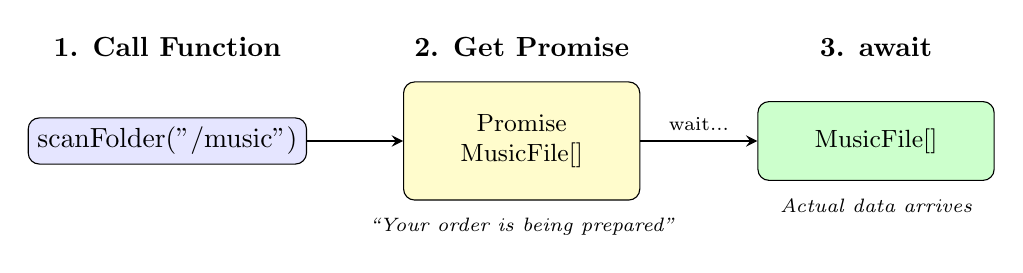
\begin{tikzpicture}[
    ticket/.style={draw, minimum width=3cm, minimum height=1.5cm, align=center, font=\small, rounded corners, fill=yellow!20},
    food/.style={draw, minimum width=3cm, minimum height=1cm, align=center, font=\small, rounded corners, fill=green!20},
    arrow/.style={->, thick, >=stealth}
]
    % Order
    \node[font=\bfseries] at (0, 2) {1. Call Function};
    \node[draw, rounded corners, fill=blue!10] (call) at (0, 0.8) {scanFolder("/music")};
    
    % Ticket
    \node[font=\bfseries] at (4.5, 2) {2. Get Promise};
    \node[ticket] (ticket) at (4.5, 0.8) {Promise\\MusicFile[]};
    \node[below=0.1cm of ticket, font=\scriptsize\itshape] {``Your order is being prepared''};
    
    % Await
    \draw[arrow] (call) -- (ticket);
    
    % Food delivered
    \node[font=\bfseries] at (9, 2) {3. await};
    \node[food] (food) at (9, 0.8) {MusicFile[]};
    \node[below=0.1cm of food, font=\scriptsize\itshape] {Actual data arrives};
    
    \draw[arrow] (ticket) -- node[above, font=\scriptsize] {wait...} (food);
\end{tikzpicture}
\caption{Promises: Order Now, Receive Later}
\label{fig:promise_ticket}
\end{figure}

When a function is \inlinecode{async}, it automatically returns a \inlinecode{Promise}. You specify what the Promise resolves to:

\begin{lstlisting}[language=TypeScript, title=Async Function Return Types]
// Promise<MusicFile[]> means: this async function 
// will eventually return an array of MusicFile objects
async function scanFolder(path: string): Promise<MusicFile[]> {
  const files = await readDirectory(path);
  return files;  // Must be MusicFile[]
}

// Promise<void> means: returns nothing (but still async)
async function saveSettings(settings: AppSettings): Promise<void> {
  await writeFile('settings.json', settings);
  // No return statement needed
}

// Usage - TypeScript knows the resolved type
const songs = await scanFolder("/music");
// TypeScript knows: songs is MusicFile[]
console.log(songs[0].title);  // Autocomplete works!
\end{lstlisting}

\subsection{How the Compiler Determines Types}

\begin{tipbox}
\textbf{Analogy: A Smart Assistant}

Type inference is like having a \textbf{smart assistant} who watches what you do. If you write \inlinecode{const age = 25}, the assistant thinks: ``They put a number in there, so 'age' must be a number.'' You don't have to explicitly say \inlinecode{const age: number = 25} --- the assistant figures it out. But if you later try to do \inlinecode{age = "old"}, the assistant says: ``Wait, you said age was a number!''
\end{tipbox}

TypeScript uses \textbf{type inference} --- it can often figure out types automatically:

\begin{lstlisting}[language=TypeScript, title=Type Inference]
// TypeScript INFERS these types automatically:
const name = "John";       // TypeScript knows: string
const count = 42;          // TypeScript knows: number
const items = ["a", "b"];  // TypeScript knows: string[]

// Function return type is inferred from the return statement
function double(n: number) {
  return n * 2;  // TypeScript infers return type: number
}

// But explicit types are BETTER for documentation:
function double(n: number): number {
  return n * 2;
}
\end{lstlisting}

\subsection{How Types Flow Through the Application}

\begin{tipbox}
\textbf{Analogy: Package Delivery}

Think of types flowing through the app like a \textbf{package delivery system}. The backend (warehouse) packs a box labeled ``MusicFile[].'' The preload script (shipping company) promises to deliver ``MusicFile[].'' The frontend (customer) receives a box and knows exactly what's inside because the label matches all the way through. If someone mislabels a box along the way, the system catches it before delivery.
\end{tipbox}

Here's the complete flow of how a type defined in the backend reaches the frontend:

\begin{figure}[ht!]
\centering
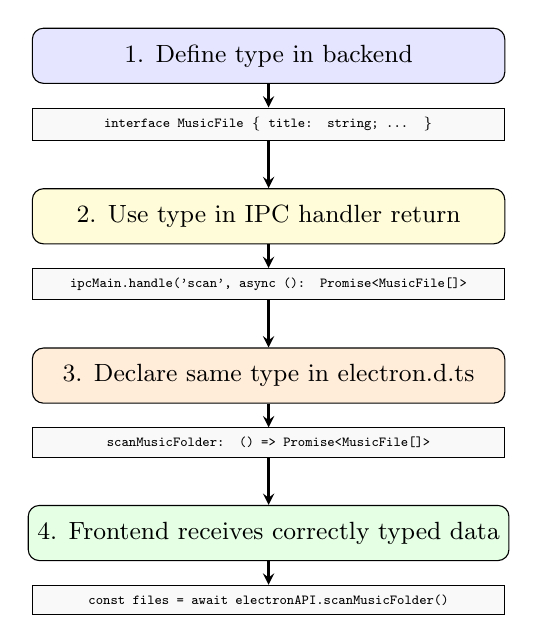
\begin{tikzpicture}[
    node distance=0.6cm,
    box/.style={draw, rounded corners, minimum width=6cm, minimum height=0.7cm, align=center, font=\small},
    code/.style={draw, rectangle, fill=gray!5, minimum width=6cm, align=left, font=\ttfamily\tiny},
    arrow/.style={->, thick, >=stealth}
]
    % Step 1
    \node[box, fill=blue!10] (define) {1. Define type in backend};
    \node[code, below=0.3cm of define] (def_code) {interface MusicFile \{ title: string; ... \}};
    
    % Step 2
    \node[box, fill=yellow!15, below=0.6cm of def_code] (handler) {2. Use type in IPC handler return};
    \node[code, below=0.3cm of handler] (handler_code) {ipcMain.handle('scan', async (): Promise<MusicFile[]>};
    
    % Step 3
    \node[box, fill=orange!15, below=0.6cm of handler_code] (dts) {3. Declare same type in electron.d.ts};
    \node[code, below=0.3cm of dts] (dts_code) {scanMusicFolder: () => Promise<MusicFile[]>};
    
    % Step 4
    \node[box, fill=green!10, below=0.6cm of dts_code] (use) {4. Frontend receives correctly typed data};
    \node[code, below=0.3cm of use] (use_code) {const files = await electronAPI.scanMusicFolder()};
    
    \draw[arrow] (define) -- (def_code);
    \draw[arrow] (def_code) -- (handler);
    \draw[arrow] (handler) -- (handler_code);
    \draw[arrow] (handler_code) -- (dts);
    \draw[arrow] (dts) -- (dts_code);
    \draw[arrow] (dts_code) -- (use);
    \draw[arrow] (use) -- (use_code);
\end{tikzpicture}
\caption{Type Flow from Backend to Frontend}
\label{fig:type_flow}
\end{figure}

\subsection{Real Example: Complete Type Chain}

Here's how types connect across files in this project:

\textbf{Step 1: Define the type} (\filepath{electron/musicScanner.ts})
\begin{lstlisting}[language=TypeScript]
export interface MusicFile {
  path: string;
  title: string;
  artist: string;
  album: string;
  duration: number;
  albumArt: string | null;
}
\end{lstlisting}

\textbf{Step 2: Use in handler} (\filepath{electron/ipc/modules/musicHandlers.ts})
\begin{lstlisting}[language=TypeScript]
import { MusicFile } from '../../musicScanner';

ipcMain.handle('scan-music-folder', 
  async (event, folderPath: string): Promise<MusicFile[]> => {
    const files = await scanMusicFolder(folderPath);
    return files;  // TypeScript checks this is MusicFile[]
  }
);
\end{lstlisting}

\textbf{Step 3: Declare for frontend} (\filepath{src/types/electron.d.ts})
\begin{lstlisting}[language=TypeScript]
interface MusicFile {
  path: string;
  title: string;
  artist: string;
  album: string;
  duration: number;
  albumArt: string | null;
}

interface ElectronAPI {
  scanMusicFolder: (path: string) => Promise<MusicFile[]>;
}
\end{lstlisting}

\textbf{Step 4: Use in React} (\filepath{src/App.tsx})
\begin{lstlisting}[language=TypeScript]
const [songs, setSongs] = useState<MusicFile[]>([]);

const handleScan = async () => {
  const files = await window.electronAPI.scanMusicFolder('/music');
  // TypeScript knows: files is MusicFile[]
  setSongs(files);
  
  // Autocomplete works for all properties:
  files.forEach(f => console.log(f.title, f.artist));
};
\end{lstlisting}

\begin{warningbox}
\textbf{The type must match in all places!} If you add a new property to \inlinecode{MusicFile} in the backend, you must also add it to \filepath{electron.d.ts}. Otherwise, the frontend won't know about it, and TypeScript will show an error if you try to access it.
\end{warningbox}

\subsection{What Happens When Types Don't Match}

\begin{tipbox}
\textbf{Analogy: Spell Check for Code}

Type checking is like \textbf{spell check in a word processor}, but for code logic. Just as spell check underlines ``teh'' because it's not a real word, TypeScript underlines \inlinecode{song.genre} because \inlinecode{genre} isn't a real property. You fix it before hitting ``send'' (running the app), not after the recipient (user) complains.
\end{tipbox}

TypeScript prevents bugs by catching mismatches at compile time:

\begin{lstlisting}[language=TypeScript, title=TypeScript Catching Errors]
// ERROR 1: Missing required property
const song: MusicFile = {
  path: "/music/song.mp3",
  title: "My Song"
  // ERROR: Property 'artist' is missing
};

// ERROR 2: Wrong property type
const song2: MusicFile = {
  path: "/music/song.mp3",
  title: "My Song",
  artist: "Artist",
  duration: "3:00",  // ERROR: string not assignable to number
  albumArt: null
};

// ERROR 3: Accessing non-existent property
console.log(song.genre);  // ERROR: Property 'genre' does not exist

// ERROR 4: Calling function with wrong argument type
scanMusicFolder(42);  // ERROR: number is not assignable to string
\end{lstlisting}

\begin{tipbox}
\textbf{Summary}: Types act as a contract between different parts of your code. The compiler is the enforcer --- it checks that everyone follows the contract at build time, before your code ever runs.
\end{tipbox}

\section{File Map: What Does What?}

\subsection{Electron Backend (Node.js)}

\begin{longtable}{@{}p{4cm}p{9.5cm}@{}}
\toprule
\textbf{File} & \textbf{Purpose} \\
\midrule
\endhead

\filepath{electron/main.ts} & \textbf{ENTRY POINT} --- Creates the app window, starts everything \\
\filepath{electron/preload.ts} & \textbf{THE BRIDGE} --- Safely exposes backend functions to frontend \\
\filepath{electron/window.ts} & Creates app window with custom title bar \\
\filepath{electron/tray.ts} & System tray icon with play/pause controls \\
\filepath{electron/musicScanner.ts} & Finds music files and reads metadata \\
\filepath{electron/parallelMetadataScanner.ts} & Multi-threaded metadata parsing \\
\filepath{electron/fileWatcher.ts} & Monitors music folder in real-time \\
\filepath{electron/metadataCache.ts} & SQLite cache for scan tracking \\
\filepath{electron/youtubeDownloader.ts} & Downloads audio from YouTube \\
\filepath{electron/playlistDatabase.ts} & SQLite database for playlists \\
\filepath{electron/whisperManager.ts} & AI transcription system \\
\filepath{electron/fpcalcManager.ts} & Audio fingerprinting \\
\filepath{electron/binaryManager.ts} & Binary status checking \\
\bottomrule
\caption{Electron Backend Files}
\end{longtable}

\subsection{IPC Handler Modules}

Located in \filepath{electron/ipc/modules/}:

\begin{table}[ht!]
\centering
\begin{tabular}{@{}p{4cm}p{8cm}@{}}
\toprule
\textbf{Module} & \textbf{Handles} \\
\midrule
\filepath{musicHandlers.ts} & Scanning folders, reading files \\
\filepath{playlistHandlers.ts} & Create/delete/update playlists \\
\filepath{youtubeHandlers.ts} & Download from YouTube, binary installs \\
\filepath{apiHandlers.ts} & External APIs (AcoustID, MusicBrainz) \\
\filepath{systemHandlers.ts} & Window controls (minimize, close) \\
\filepath{cacheHandlers.ts} & Metadata database operations \\
\filepath{fingerprintHandlers.ts} & Audio fingerprinting (fpcalc) \\
\filepath{lyricsHandlers.ts} & Vocal isolation + AI transcription \\
\filepath{watchHandlers.ts} & File system watching \\
\bottomrule
\end{tabular}
\caption{IPC Handler Modules}
\end{table}

\section{How Data Flows: Playing a Song}

\begin{enumerate}
    \item \textbf{User clicks a song in SongList.tsx}
    \begin{itemize}
        \item Calls \inlinecode{onPlaySong(file, index)}
    \end{itemize}
    
    \item \textbf{App.tsx receives the call}
    \begin{itemize}
        \item Calls \inlinecode{playSong(file, index)} from \inlinecode{useAudioPlayer} hook
    \end{itemize}
    
    \item \textbf{useAudioPlayer.ts processes the request}
    \begin{itemize}
        \item Creates new \inlinecode{Howl(\{ src: 'file://path/to/song.mp3' \})}
        \item Calls \inlinecode{sound.play()}
        \item Updates state: \inlinecode{setIsPlaying(true)}
    \end{itemize}
    
    \item \textbf{React re-renders}
    \begin{itemize}
        \item PlaybackBar shows the song title, artist, album art
        \item SongList highlights the playing song
        \item AudioVisualizer starts animating
    \end{itemize}
\end{enumerate}

\begin{figure}[ht!]
    \centering
    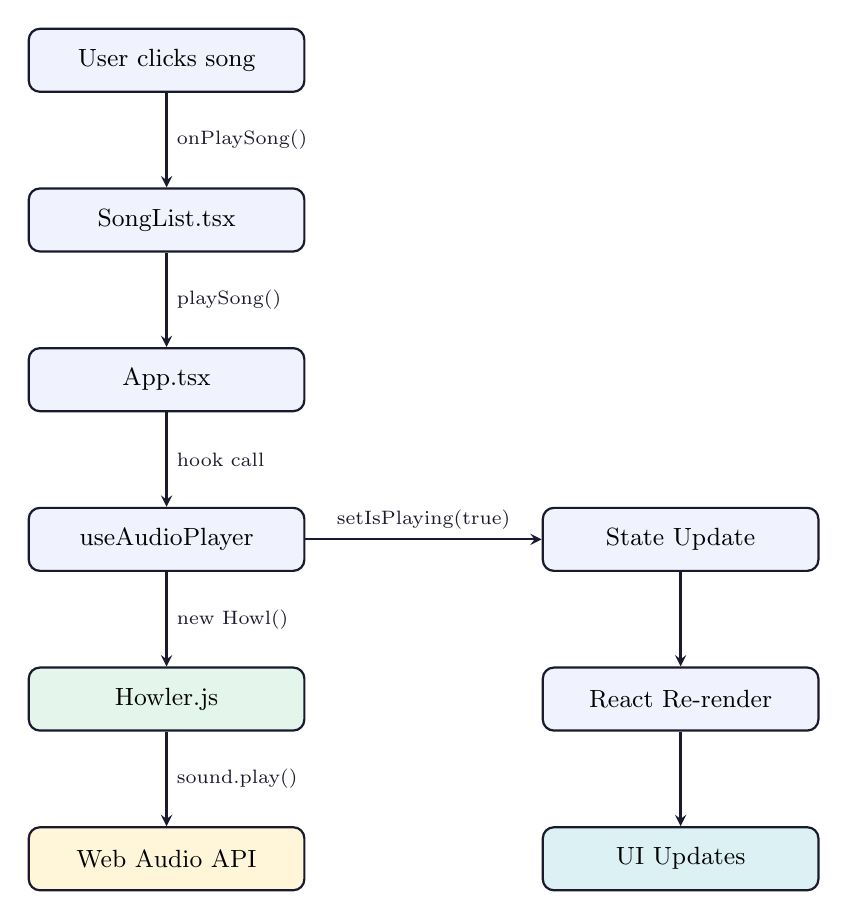
\begin{tikzpicture}[
        node distance=1.2cm,
        flowstep/.style={rectangle, rounded corners, draw=sectioncolor, fill=accentcolor!10, thick, minimum width=3.5cm, minimum height=0.8cm, align=center, font=\small},
        arrow/.style={thick, ->, >=stealth, sectioncolor}
    ]
        % Flow steps
        \node (click) [flowstep] {User clicks song};
        \node (songlist) [flowstep, below=of click] {SongList.tsx};
        \node (app) [flowstep, below=of songlist] {App.tsx};
        \node (hook) [flowstep, below=of app] {useAudioPlayer};
        \node (howler) [flowstep, below=of hook, fill=successcolor!15] {Howler.js};
        \node (audio) [flowstep, below=of howler, fill=warningcolor!15] {Web Audio API};
        
        % Arrows
        \draw [arrow] (click) -- node[right, font=\scriptsize] {onPlaySong()} (songlist);
        \draw [arrow] (songlist) -- node[right, font=\scriptsize] {playSong()} (app);
        \draw [arrow] (app) -- node[right, font=\scriptsize] {hook call} (hook);
        \draw [arrow] (hook) -- node[right, font=\scriptsize] {new Howl()} (howler);
        \draw [arrow] (howler) -- node[right, font=\scriptsize] {sound.play()} (audio);
        
        % UI updates branch
        \node (state) [flowstep, right=3cm of hook] {State Update};
        \node (rerender) [flowstep, below=of state] {React Re-render};
        \node (ui) [flowstep, below=of rerender, fill=infocolor!15] {UI Updates};
        
        \draw [arrow] (hook) -- node[above, font=\scriptsize] {setIsPlaying(true)} (state);
        \draw [arrow] (state) -- (rerender);
        \draw [arrow] (rerender) -- (ui);
    \end{tikzpicture}
    \caption{Audio Playback Data Flow}
    \label{fig:playback_flow}
\end{figure}

% Playback Ecosystem Diagram
\begin{figure}[ht!]
\centering
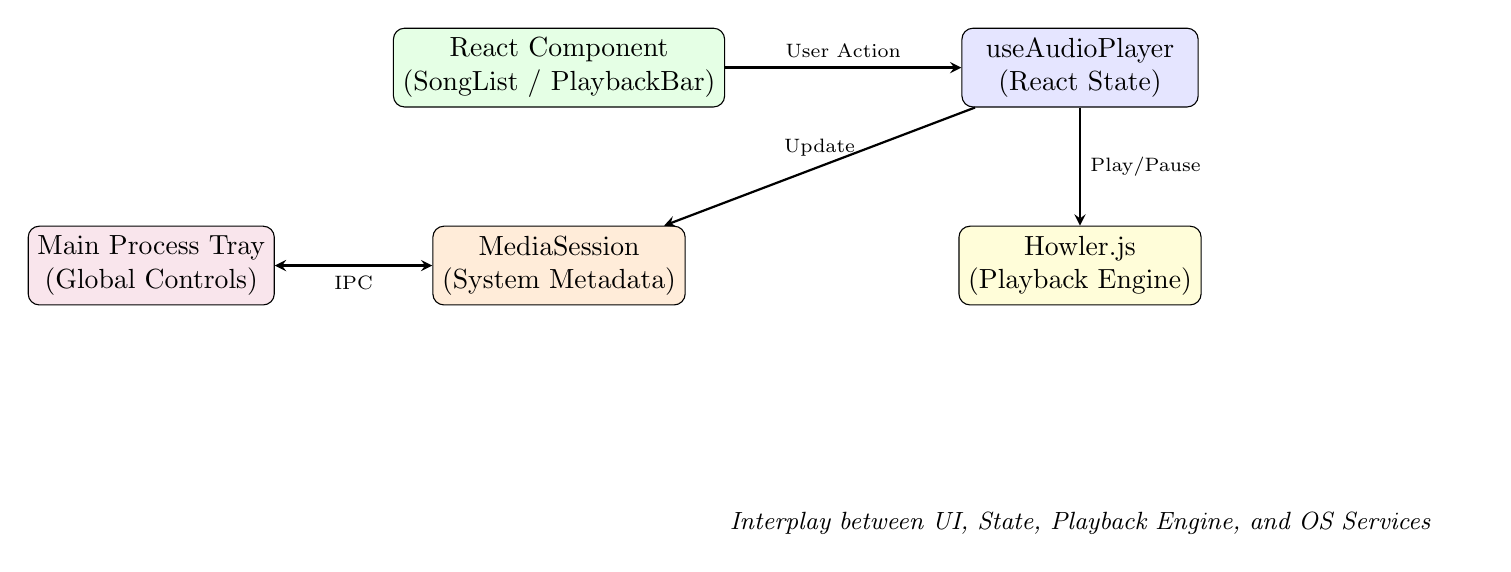
\begin{tikzpicture}[
    node distance=1.5cm,
    component/.style={draw, rounded corners, minimum width=3cm, minimum height=1cm, align=center, fill=white},
    arrow/.style={->, thick, >=stealth}
]
    % Main components
    \node[component, fill=green!10] (react) {React Component\\(SongList / PlaybackBar)};
    \node[component, fill=blue!10, right=3cm of react] (hook) {useAudioPlayer\\(React State)};
    \node[component, fill=yellow!15, below=of hook] (howler) {Howler.js\\(Playback Engine)};
    \node[component, fill=orange!15, below=of react] (media) {MediaSession\\(System Metadata)};
    \node[component, fill=purple!10, left=2cm of media] (tray) {Main Process Tray\\(Global Controls)};
    
    % Arrows
    \draw[arrow] (react) -- node[above, font=\scriptsize] {User Action} (hook);
    \draw[arrow] (hook) -- node[right, font=\scriptsize] {Play/Pause} (howler);
    \draw[arrow] (hook) -- node[above, font=\scriptsize] {Update} (media);
    \draw[arrow, <->] (tray) -- node[below, font=\scriptsize] {IPC} (media);
    
    % Caption below
    \node[below=2.5cm of howler, text width=10cm, align=center, font=\small\itshape] {Interplay between UI, State, Playback Engine, and OS Services};
\end{tikzpicture}
\caption{Playback Ecosystem: State Synchronization and OS Integration}
\label{fig:playback_ecosystem}
\end{figure}

% MediaSession API Integration Diagram
\begin{figure}[ht!]
\centering
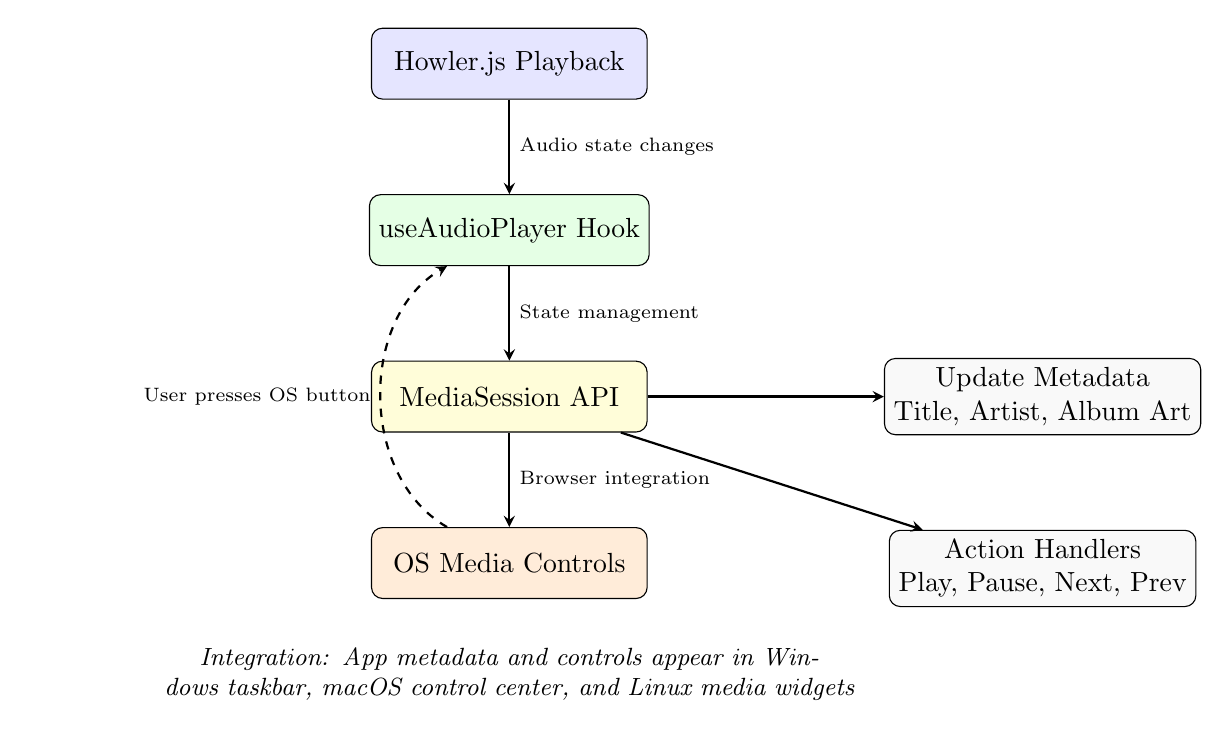
\begin{tikzpicture}[
    node distance=1.2cm,
    box/.style={draw, rounded corners, minimum width=3.5cm, minimum height=0.9cm, align=center, fill=white},
    arrow/.style={->, thick, >=stealth}
]
    % Left column - App side
    \node[box, fill=blue!10] (howler) {Howler.js Playback};
    \node[box, fill=green!10, below=of howler] (hook) {useAudioPlayer Hook};
    \node[box, fill=yellow!15, below=of hook] (mediasession) {MediaSession API};
    \node[box, fill=orange!15, below=of mediasession] (os) {OS Media Controls};
    
    % Right column - Details
    \node[box, fill=gray!5, right=3cm of mediasession] (metadata) {Update Metadata\\Title, Artist, Album Art};
    \node[box, fill=gray!5, below=of metadata] (handlers) {Action Handlers\\Play, Pause, Next, Prev};
    
    % Arrows
    \draw[arrow] (howler) -- node[right, font=\scriptsize] {Audio state changes} (hook);
    \draw[arrow] (hook) -- node[right, font=\scriptsize] {State management} (mediasession);
    \draw[arrow] (mediasession) -- node[right, font=\scriptsize] {Browser integration} (os);
    \draw[arrow] (mediasession) -- (metadata);
    \draw[arrow] (mediasession) -- (handlers);
    \draw[arrow, dashed] (os) to[bend left=60] node[left, font=\scriptsize] {User presses OS button} (hook);
    
    % Note
    \node[below=0.5cm of os, text width=12cm, align=center, font=\small\itshape] {Integration: App metadata and controls appear in Windows taskbar, macOS control center, and Linux media widgets};
\end{tikzpicture}
\caption{MediaSession API Integration: OS-Level Media Controls Synchronization}
\label{fig:mediasession}
\end{figure}

%%%%%%%%%%%%%%%%%%%%%%%%%%%%%%%%%%%%%%%%%%%%%%%%%%%%%%%%%%%%%%%%%%%%%%%%%%%%%%%
% CHAPTER 2: OVERVIEW
%%%%%%%%%%%%%%%%%%%%%%%%%%%%%%%%%%%%%%%%%%%%%%%%%%%%%%%%%%%%%%%%%%%%%%%%%%%%%%%
\chapter{Overview}
\label{ch:overview}

This is an \textbf{Electron + React + TypeScript} desktop music player application. It allows users to:

\begin{itemize}
    \item Browse and play local music files
    \item Download music from YouTube using \inlinecode{yt-dlp}
    \item Control playback from the system tray
    \item Identify songs using audio fingerprinting (AcoustID + MusicBrainz)
    \item Custom frameless window with a soft blue title bar
    \item Filter library by artist/album via sidebar
    \item Create and manage playlists
    \item Generate AI-powered lyrics using Whisper transcription
\end{itemize}

% Overview diagrams grid
\begin{figure}[ht!]
\centering
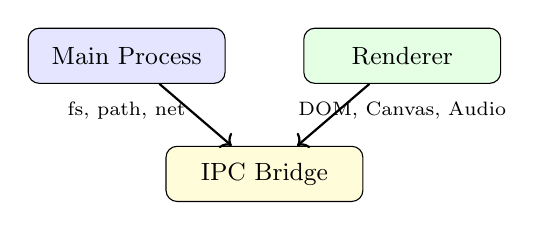
\begin{tikzpicture}[
    box/.style={draw, rounded corners, minimum width=2.5cm, minimum height=0.7cm, align=center, font=\small}
]
    % Node.js vs Browser APIs
    \node[box, fill=blue!10] at (0,0) (main) {Main Process};
    \node[font=\scriptsize, below=0.1cm of main] {fs, path, net};
    \node[box, fill=green!10] at (3.5,0) (renderer) {Renderer};
    \node[font=\scriptsize, below=0.1cm of renderer] {DOM, Canvas, Audio};
    \node[box, fill=yellow!15] at (1.75,-1.5) (bridge) {IPC Bridge};
    \draw[->, thick] (main) -- (bridge);
    \draw[->, thick] (renderer) -- (bridge);
\end{tikzpicture}
\caption{Node.js vs Browser APIs}
\label{fig:nodejs_browser}
\end{figure}

\begin{figure}[ht!]
\centering
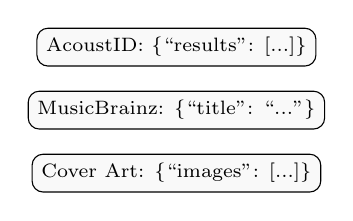
\begin{tikzpicture}[
    box/.style={draw, rounded corners, minimum width=3cm, align=center, font=\scriptsize, fill=gray!5}
]
    \node[box] at (0,0) {AcoustID: \{``results'': [...]\}};
    \node[box] at (0,-0.8) {MusicBrainz: \{``title'': ``...''\}};
    \node[box] at (0,-1.6) {Cover Art: \{``images'': [...]\}};
\end{tikzpicture}
\caption{API Response Examples}
\label{fig:api_responses}
\end{figure}

\begin{figure}[ht!]
\centering
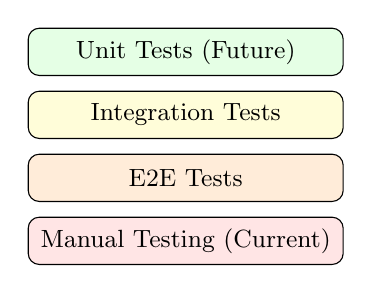
\begin{tikzpicture}[
    layer/.style={draw, rounded corners, minimum width=4cm, minimum height=0.6cm, align=center, font=\small}
]
    \node[layer, fill=green!10] at (0,0) {Unit Tests (Future)};
    \node[layer, fill=yellow!15] at (0,-0.8) {Integration Tests};
    \node[layer, fill=orange!15] at (0,-1.6) {E2E Tests};
    \node[layer, fill=red!10] at (0,-2.4) {Manual Testing (Current)};
\end{tikzpicture}
\caption{Testing Strategy}
\label{fig:testing_pyramid}
\end{figure}

\begin{figure}[ht!]
\centering
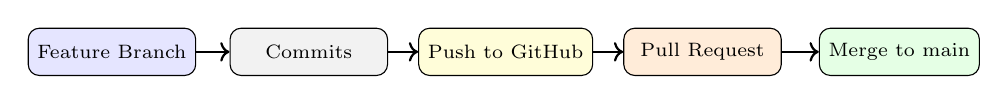
\begin{tikzpicture}[
    box/.style={draw, rounded corners, minimum width=2cm, minimum height=0.6cm, align=center, font=\scriptsize},
    arrow/.style={->, thick}
]
    \node[box, fill=blue!10] at (0,0) (branch) {Feature Branch};
    \node[box, fill=gray!10] at (2.5,0) (commits) {Commits};
    \node[box, fill=yellow!15] at (5,0) (push) {Push to GitHub};
    \node[box, fill=orange!15] at (7.5,0) (pr) {Pull Request};
    \node[box, fill=green!10] at (10,0) (merge) {Merge to main};
    \draw[arrow] (branch) -- (commits);
    \draw[arrow] (commits) -- (push);
    \draw[arrow] (push) -- (pr);
    \draw[arrow] (pr) -- (merge);
\end{tikzpicture}
\caption{Git Workflow}
\label{fig:git_workflow}
\end{figure}

\begin{figure}[ht!]
\centering
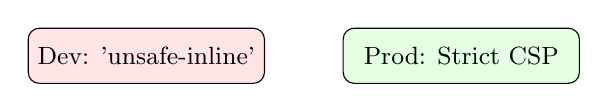
\begin{tikzpicture}[
    box/.style={draw, rounded corners, minimum width=3cm, minimum height=0.7cm, align=center, font=\small}
]
    \node[box, fill=red!10] at (0,0) {Dev: 'unsafe-inline'};
    \node[box, fill=green!10] at (4,0) {Prod: Strict CSP};
\end{tikzpicture}
\caption{CSP Configuration}
\label{fig:csp_config}
\end{figure}

\begin{figure}[ht!]
\centering
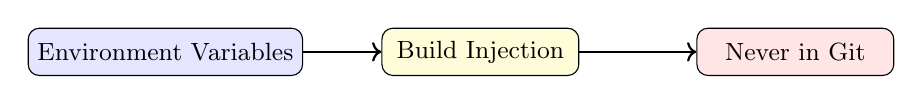
\begin{tikzpicture}[
    box/.style={draw, rounded corners, minimum width=2.5cm, minimum height=0.6cm, align=center, font=\small},
    arrow/.style={->, thick}
]
    \node[box, fill=blue!10] at (0,0) (env) {Environment Variables};
    \node[box, fill=yellow!15] at (4,0) (build) {Build Injection};
    \node[box, fill=red!10] at (8,0) (git) {Never in Git};
    \draw[arrow] (env) -- (build);
    \draw[arrow] (build) -- (git);
\end{tikzpicture}
\caption{API Key Management}
\label{fig:api_keys}
\end{figure}

\begin{figure}[ht!]
\centering
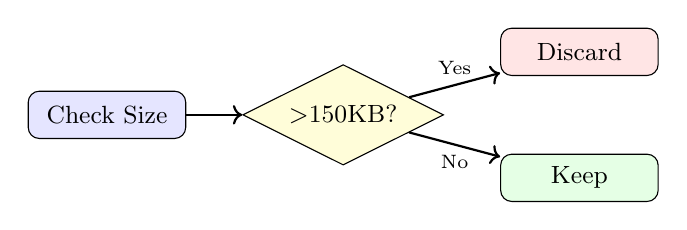
\begin{tikzpicture}[
    box/.style={draw, rounded corners, minimum width=2cm, minimum height=0.6cm, align=center, font=\small},
    decision/.style={draw, diamond, aspect=2, fill=yellow!15, font=\small},
    arrow/.style={->, thick}
]
    \node[box, fill=blue!10] at (0,0) (check) {Check Size};
    \node[decision] at (3,0) (size) {$>$150KB?};
    \node[box, fill=red!10] at (6,0.8) (discard) {Discard};
    \node[box, fill=green!10] at (6,-0.8) (keep) {Keep};
    \draw[arrow] (check) -- (size);
    \draw[arrow] (size) -- node[above, font=\scriptsize] {Yes} (discard);
    \draw[arrow] (size) -- node[below, font=\scriptsize] {No} (keep);
\end{tikzpicture}
\caption{Album Art Size Optimization}
\label{fig:album_art_size}
\end{figure}

\begin{figure}[ht!]
\centering
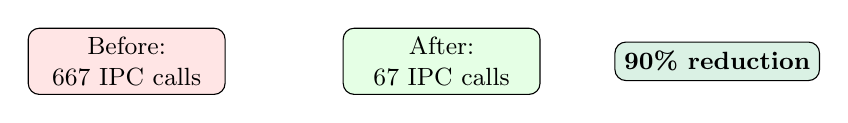
\begin{tikzpicture}[
    box/.style={draw, rounded corners, minimum width=2.5cm, minimum height=0.7cm, align=center, font=\small}
]
    \node[box, fill=red!10] at (0,0) {Before:\\667 IPC calls};
    \node[box, fill=green!10] at (4,0) {After:\\67 IPC calls};
    \node[font=\small\bfseries, fill=successcolor!20, draw, rounded corners] at (7.5,0) {90\% reduction};
\end{tikzpicture}
\caption{Batch IPC Optimization}
\label{fig:batch_ipc}
\end{figure}

\begin{figure}[ht!]
\centering
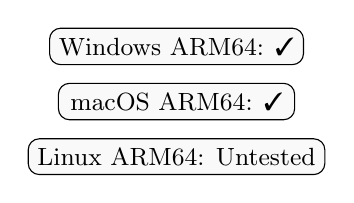
\begin{tikzpicture}[
    box/.style={draw, rounded corners, minimum width=3cm, align=center, font=\small, fill=gray!5}
]
    \node[box] at (0,0) {Windows ARM64: \cmark};
    \node[box] at (0,-0.7) {macOS ARM64: \cmark};
    \node[box] at (0,-1.4) {Linux ARM64: Untested};
\end{tikzpicture}
\caption{ARM64 Support Status}
\label{fig:arm64_support}
\end{figure}

\begin{figure}[ht!]
\centering
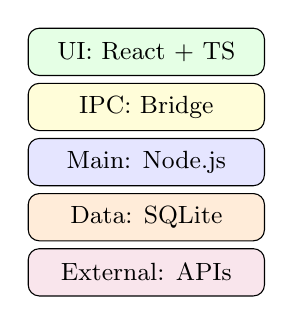
\begin{tikzpicture}[
    layer/.style={draw, rounded corners, minimum width=3cm, minimum height=0.6cm, align=center, font=\small}
]
    \node[layer, fill=green!10] at (0,0) {UI: React + TS};
    \node[layer, fill=yellow!15] at (0,-0.7) {IPC: Bridge};
    \node[layer, fill=blue!10] at (0,-1.4) {Main: Node.js};
    \node[layer, fill=orange!15] at (0,-2.1) {Data: SQLite};
    \node[layer, fill=purple!10] at (0,-2.8) {External: APIs};
\end{tikzpicture}
\caption{Technology Stack Layers}
\label{fig:tech_layers}
\end{figure}

\begin{figure}[ht!]
\centering
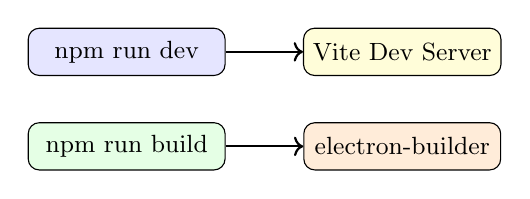
\begin{tikzpicture}[
    box/.style={draw, rounded corners, minimum width=2.5cm, minimum height=0.6cm, align=center, font=\small},
    arrow/.style={->, thick}
]
    \node[box, fill=blue!10] at (0,0) (dev) {npm run dev};
    \node[box, fill=yellow!15] at (3.5,0) (vite) {Vite Dev Server};
    \node[box, fill=green!10] at (0,-1.2) (build) {npm run build};
    \node[box, fill=orange!15] at (3.5,-1.2) (electron) {electron-builder};
    \draw[arrow] (dev) -- (vite);
    \draw[arrow] (build) -- (electron);
\end{tikzpicture}
\caption{Build Process Flow}
\label{fig:build_process}
\end{figure}

\section{Tech Stack}

\begin{longtable}{@{}p{3.5cm}p{4.5cm}p{6cm}@{}}
\toprule
\textbf{Layer} & \textbf{Technology} & \textbf{Purpose} \\
\midrule
\endhead

Runtime & Electron 39 & Desktop app framework \\
Frontend & React 18 + TypeScript & UI components \\
Build Tool & Vite 7 & Fast dev server and bundling \\
Audio Playback & Howler.js & Cross-platform audio \\
Metadata & music-metadata & Extract ID3 tags and album art \\
YouTube & yt-dlp-wrap & Download audio from YouTube \\
Audio Fingerprinting & fpcalc (Chromaprint) & Generate audio fingerprints \\
Audio Processing & FFmpeg & Vocal isolation, format conversion \\
AI Transcription & Whisper.cpp & Speech-to-text for lyrics \\
Tag Writing & taglib-wasm & Write cover art to files \\
Database & better-sqlite3 & SQLite metadata cache \\
Sliders & rc-slider & Seek bar and volume control \\
Scrollbars & overlayscrollbars-react & Custom themed scrollbars \\
HTTP & axios & API requests \\
Styling & CSS (no framework) & Custom responsive design \\
\bottomrule
\caption{Technology Stack}
\end{longtable}

\section{Supported Audio Formats}

\filepath{.mp3}, \filepath{.flac}, \filepath{.wav}, \filepath{.m4a}, \filepath{.aac}, \filepath{.ogg}, \filepath{.opus}, \filepath{.wma}, \filepath{.aiff}, \filepath{.mp4}, \filepath{.m4p}, \filepath{.amr}

\section{Directory Structure}

\begin{lstlisting}
music-electron-app/
+-- electron/                 # Main Process (Node.js)
|   +-- main.ts              # App entry point
|   +-- preload.ts           # IPC bridge
|   +-- window.ts            # Window creation
|   +-- tray.ts              # System tray
|   +-- musicScanner.ts      # File discovery
|   +-- metadataCache.ts     # SQLite scan cache
|   +-- playlistDatabase.ts  # SQLite playlists
|   +-- youtubeDownloader.ts # yt-dlp wrapper
|   +-- fpcalcManager.ts     # Audio fingerprinting
|   +-- whisperManager.ts    # AI transcription
|   +-- settings.ts          # Settings persistence
|   +-- ipc/
|       +-- handlers.ts      # Handler registry
|       +-- modules/         # Feature-specific handlers
+-- src/                     # Renderer Process (React)
|   +-- main.tsx            # React entry
|   +-- App.tsx             # Main component
|   +-- hooks/              # Custom React hooks
|   +-- components/         # UI components
|   |   +-- layout/         # TitleBar, Sidebar, PlaybackBar
|   |   +-- library/        # SongList, BatchScanProgress
|   |   +-- playlists/      # PlaylistList, CreatePlaylistModal
|   |   +-- lyrics/         # LyricsPanel
|   |   +-- common/         # AudioVisualizer, ContextMenu
|   |   +-- settings/       # Settings modal
|   |   +-- download/       # DownloadButton, Notification
|   +-- services/           # API wrappers
|   +-- utils/              # Helper functions
|   +-- assets/icons/       # 39 custom SVG icons
+-- package.json
+-- vite.config.ts
+-- electron-builder.json5
\end{lstlisting}

% SQL Query Collection diagram
\begin{figure}[ht!]
\centering
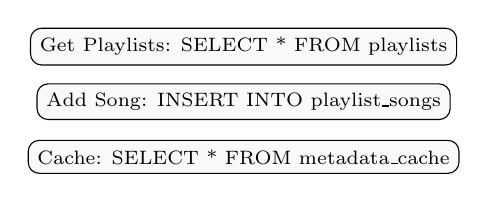
\begin{tikzpicture}[
    box/.style={draw, rounded corners, minimum width=5cm, align=center, font=\scriptsize, fill=gray!5}
]
    \node[box] at (0,0) {Get Playlists: SELECT * FROM playlists};
    \node[box] at (0,-0.7) {Add Song: INSERT INTO playlist\_songs};
    \node[box] at (0,-1.4) {Cache: SELECT * FROM metadata\_cache};
\end{tikzpicture}
\caption{SQL Query Collection}
\label{fig:sql_queries}
\end{figure}

% First-Time User Onboarding Flow
\begin{figure}[ht!]
\centering
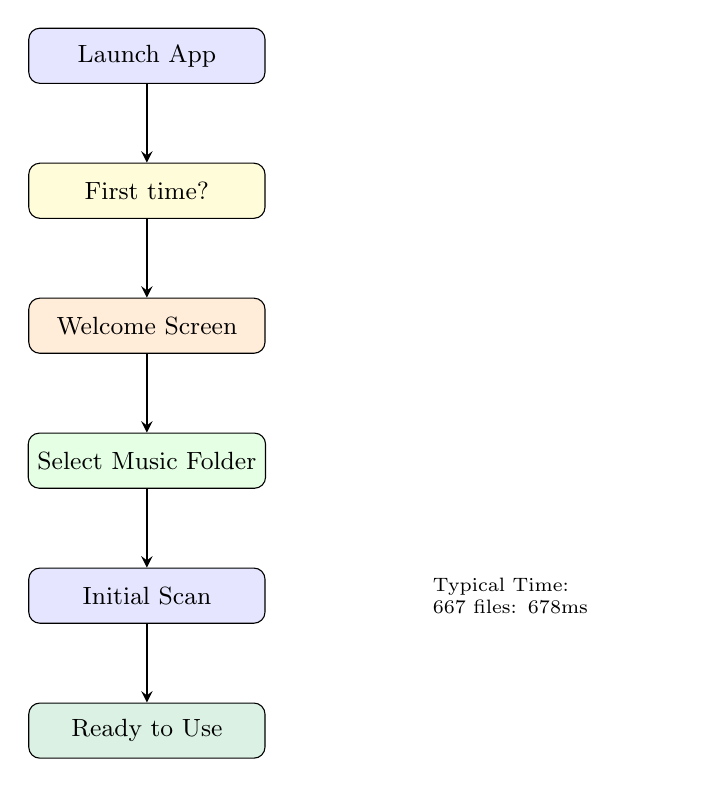
\begin{tikzpicture}[
    node distance=1cm,
    box/.style={draw, rounded corners, minimum width=3cm, minimum height=0.7cm, align=center, font=\small},
    arrow/.style={->, thick, >=stealth}
]
    \node[box, fill=blue!10] (launch) {Launch App};
    \node[box, fill=yellow!15, below=of launch] (first) {First time?};
    \node[box, fill=orange!15, below=of first] (welcome) {Welcome Screen};
    \node[box, fill=green!10, below=of welcome] (select) {Select Music Folder};
    \node[box, fill=blue!10, below=of select] (scan) {Initial Scan};
    \node[box, fill=successcolor!20, below=of scan] (ready) {Ready to Use};
    
    \draw[arrow] (launch) -- (first);
    \draw[arrow] (first) -- (welcome);
    \draw[arrow] (welcome) -- (select);
    \draw[arrow] (select) -- (scan);
    \draw[arrow] (scan) -- (ready);
    
    \node[right=2cm of scan, text width=3cm, font=\scriptsize, align=left] {Typical Time:\\667 files: 678ms};
\end{tikzpicture}
\caption{First-Time User Onboarding: Initial Setup and Library Scan Flow}
\label{fig:onboarding}
\end{figure}

% Technology Stack Layered Architecture
\begin{figure}[ht!]
\centering
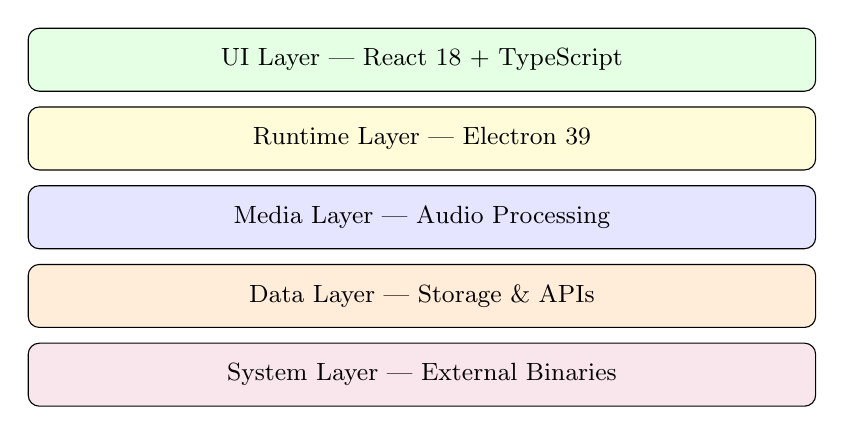
\begin{tikzpicture}[
    layer/.style={draw, rounded corners, minimum width=10cm, minimum height=0.8cm, align=center, font=\small}
]
    \node[layer, fill=green!10] at (0,0) {UI Layer --- React 18 + TypeScript};
    \node[layer, fill=yellow!15] at (0,-1) {Runtime Layer --- Electron 39};
    \node[layer, fill=blue!10] at (0,-2) {Media Layer --- Audio Processing};
    \node[layer, fill=orange!15] at (0,-3) {Data Layer --- Storage \& APIs};
    \node[layer, fill=purple!10] at (0,-4) {System Layer --- External Binaries};
\end{tikzpicture}
\caption{Technology Stack Layered Architecture}
\label{fig:tech_stack_layers}
\end{figure}

% YouTube Search and Acquisition Flow
\begin{figure}[ht!]
\centering
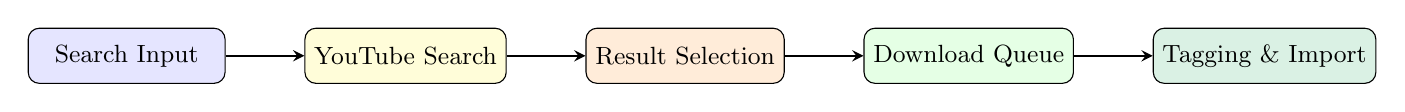
\begin{tikzpicture}[
    node distance=1cm,
    box/.style={draw, rounded corners, minimum width=2.5cm, minimum height=0.7cm, align=center, font=\small},
    arrow/.style={->, thick, >=stealth}
]
    \node[box, fill=blue!10] (search) {Search Input};
    \node[box, fill=yellow!15, right=of search] (yt) {YouTube Search};
    \node[box, fill=orange!15, right=of yt] (result) {Result Selection};
    \node[box, fill=green!10, right=of result] (download) {Download Queue};
    \node[box, fill=successcolor!20, right=of download] (tag) {Tagging \& Import};
    
    \draw[arrow] (search) -- (yt);
    \draw[arrow] (yt) -- (result);
    \draw[arrow] (result) -- (download);
    \draw[arrow] (download) -- (tag);
\end{tikzpicture}
\caption{YouTube Search and Acquisition Flow}
\label{fig:youtube_search}
\end{figure}

% YouTube Download to Library Pipeline
\begin{figure}[ht!]
\centering
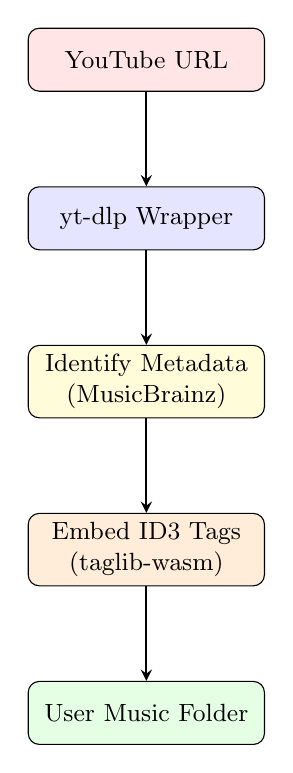
\begin{tikzpicture}[
    node distance=1.2cm,
    box/.style={draw, rounded corners, minimum width=3cm, minimum height=0.8cm, align=center, font=\small},
    arrow/.style={->, thick, >=stealth}
]
    \node[box, fill=red!10] (url) {YouTube URL};
    \node[box, fill=blue!10, below=of url] (ytdlp) {yt-dlp Wrapper};
    \node[box, fill=yellow!15, below=of ytdlp] (metadata) {Identify Metadata\\(MusicBrainz)};
    \node[box, fill=orange!15, below=of metadata] (embed) {Embed ID3 Tags\\(taglib-wasm)};
    \node[box, fill=green!10, below=of embed] (folder) {User Music Folder};
    
    \draw[arrow] (url) -- (ytdlp);
    \draw[arrow] (ytdlp) -- (metadata);
    \draw[arrow] (metadata) -- (embed);
    \draw[arrow] (embed) -- (folder);
\end{tikzpicture}
\caption{YouTube Download to Library Pipeline}
\label{fig:youtube_pipeline}
\end{figure}

\begin{notebox}
\textbf{Rate Limiting (youtubeDownloader.ts):}
\begin{lstlisting}
const DOWNLOAD_DELAY_MS = 10000; // 10 seconds

// Enforce minimum delay between downloads
const timeSinceLastDownload = Date.now() - lastDownloadTime;
if (timeSinceLastDownload < DOWNLOAD_DELAY_MS) {
  await sleep(DOWNLOAD_DELAY_MS - timeSinceLastDownload);
}
\end{lstlisting}
This prevents hitting YouTube rate limits and potential IP blocks.
\end{notebox}

%%%%%%%%%%%%%%%%%%%%%%%%%%%%%%%%%%%%%%%%%%%%%%%%%%%%%%%%%%%%%%%%%%%%%%%%%%%%%%%
% CHAPTER 3: ARCHITECTURE
%%%%%%%%%%%%%%%%%%%%%%%%%%%%%%%%%%%%%%%%%%%%%%%%%%%%%%%%%%%%%%%%%%%%%%%%%%%%%%%
\chapter{High-Level Architecture}
\label{ch:architecture}

\section{Two-Process Architecture}

\begin{figure}[h!]
\centering
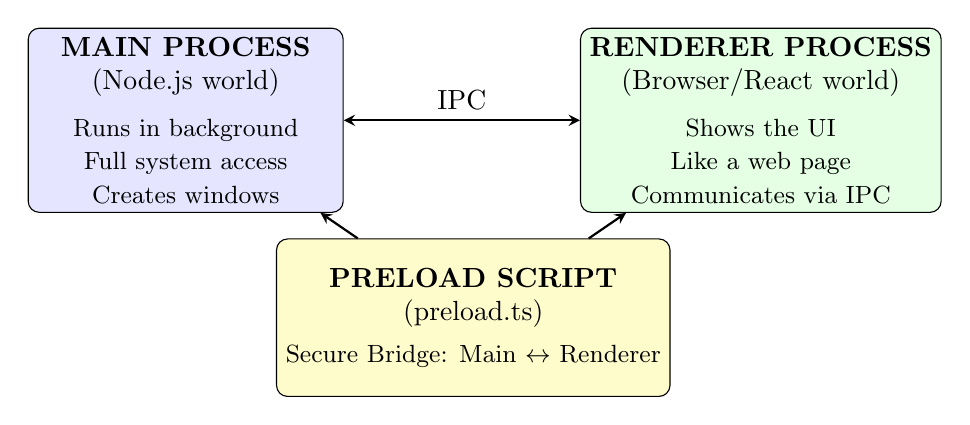
\begin{tikzpicture}[
    node distance=2cm,
    box/.style={draw, rounded corners, minimum width=4cm, minimum height=2cm, align=center, fill=white},
    arrow/.style={->, thick, >=stealth}
]
    % Main Process
    \node[box, fill=blue!10] (main) {
        \textbf{MAIN PROCESS}\\
        (Node.js world)\\[0.5em]
        \small Runs in background\\
        \small Full system access\\
        \small Creates windows
    };
    
    % Renderer Process
    \node[box, fill=green!10, right=3cm of main] (renderer) {
        \textbf{RENDERER PROCESS}\\
        (Browser/React world)\\[0.5em]
        \small Shows the UI\\
        \small Like a web page\\
        \small Communicates via IPC
    };
    
    % IPC Arrow
    \draw[arrow, <->] (main) -- node[above] {IPC} (renderer);
    
    % Preload Script
    \node[box, fill=yellow!20, below=1.5cm of $(main)!0.5!(renderer)$] (preload) {
        \textbf{PRELOAD SCRIPT}\\
        (preload.ts)\\[0.3em]
        \small Secure Bridge: Main $\leftrightarrow$ Renderer
    };
    
    \draw[arrow] (preload) -- (main);
    \draw[arrow] (preload) -- (renderer);
    
\end{tikzpicture}
\caption{Electron Two-Process Architecture}
\end{figure}

%%%%%%%%%%%%%%%%%%%%%%%%%%%%%%%%%%%%%%%%%%%%%%%%%%%%%%%%%%%%%%%%%%%%%%%%%%%%%%%
% CHAPTER 4: IPC COMMUNICATION
%%%%%%%%%%%%%%%%%%%%%%%%%%%%%%%%%%%%%%%%%%%%%%%%%%%%%%%%%%%%%%%%%%%%%%%%%%%%%%%
\chapter{IPC Communication}
\label{ch:ipc}

IPC (Inter-Process Communication) is how Electron's two worlds talk to each other. This chapter explains it step-by-step for beginners.

\section{What is IPC? (For Beginners)}

\begin{tipbox}
\textbf{Think of it like a phone call:}
\begin{itemize}
    \item The \textbf{Renderer} (React UI) wants to read files from disk
    \item But React runs in a browser-like sandbox --- it \textbf{cannot} access the file system
    \item So it must \textbf{ask} the Main Process to do it
    \item IPC is the ``phone'' that connects them
\end{itemize}
\end{tipbox}

\section{The Three Key Functions}

\begin{figure}[ht!]
\centering
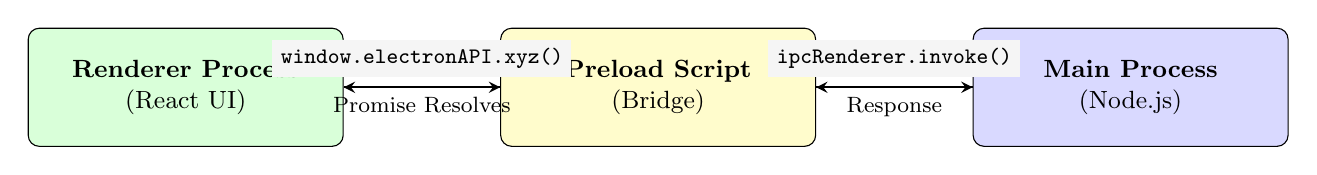
\begin{tikzpicture}[
    box/.style={draw, rounded corners, minimum width=4cm, minimum height=1.5cm, align=center, font=\small},
    arrow/.style={->, thick, >=stealth}
]
    % Three boxes
    \node[box, fill=green!15] (renderer) at (0, 0) {\textbf{Renderer Process}\\(React UI)};
    \node[box, fill=yellow!20] (preload) at (6, 0) {\textbf{Preload Script}\\(Bridge)};
    \node[box, fill=blue!15] (main) at (12, 0) {\textbf{Main Process}\\(Node.js)};
    
    % Arrows with labels
    \draw[arrow] (renderer) -- node[above, font=\footnotesize] {\inlinecode{window.electronAPI.xyz()}} (preload);
    \draw[arrow] (preload) -- node[above, font=\footnotesize] {\inlinecode{ipcRenderer.invoke()}} (main);
    \draw[arrow, dashed] (main) -- node[below, font=\footnotesize] {Response} (preload);
    \draw[arrow, dashed] (preload) -- node[below, font=\footnotesize] {Promise Resolves} (renderer);
\end{tikzpicture}
\caption{IPC Communication Flow}
\end{figure}

\subsection{1. contextBridge.exposeInMainWorld() --- The Bridge Builder}

\textbf{Location:} \filepath{preload.ts}

This function \textbf{creates a safe API} that the Renderer can access.

\begin{lstlisting}[language=TypeScript, title=preload.ts]
import { contextBridge, ipcRenderer } from 'electron';

// THIS creates window.electronAPI in the browser
contextBridge.exposeInMainWorld('electronAPI', {
  // Each method here becomes available to React
  scanMusicFolder: (path) => ipcRenderer.invoke('scan-music-folder', path),
  selectMusicFolder: () => ipcRenderer.invoke('select-music-folder'),
});
\end{lstlisting}

\begin{notebox}
\textbf{Why ``exposeInMainWorld''?}

The name means: ``Expose these functions in the main JavaScript world (the browser window).'' After this call, \inlinecode{window.electronAPI} exists in React and can be called like any JavaScript object.
\end{notebox}

\subsection{2. ipcRenderer.invoke() --- The Request Sender}

\textbf{Location:} \filepath{preload.ts} (inside the exposed methods)

This function \textbf{sends a request} to the Main Process and \textbf{waits for a response}.

\begin{lstlisting}[language=TypeScript]
// Renderer (via preload) sends a request:
const files = await ipcRenderer.invoke('scan-music-folder', '/path/to/music');
// ^^ This waits until Main Process responds
\end{lstlisting}

\textbf{Key Points:}
\begin{itemize}
    \item \inlinecode{'scan-music-folder'} is the \textbf{channel name} (like a radio frequency)
    \item \inlinecode{'/path/to/music'} is the \textbf{argument} being sent
    \item Returns a \textbf{Promise} that resolves when Main responds
\end{itemize}

\subsection{3. ipcMain.handle() --- The Request Handler}

\textbf{Location:} \filepath{electron/ipc/modules/*.ts}

This function \textbf{listens for requests} on a channel and \textbf{processes them}.

\begin{lstlisting}[language=TypeScript, title=musicHandlers.ts]
import { ipcMain } from 'electron';

// Register a handler for the 'scan-music-folder' channel
ipcMain.handle('scan-music-folder', async (event, folderPath) => {
  // This code runs in the Main Process (full Node.js access!)
  const files = await scanDirectory(folderPath);
  return files; // This becomes the Promise result in Renderer
});
\end{lstlisting}

\section{Complete IPC Request Lifecycle}

\begin{figure}[ht!]
\centering
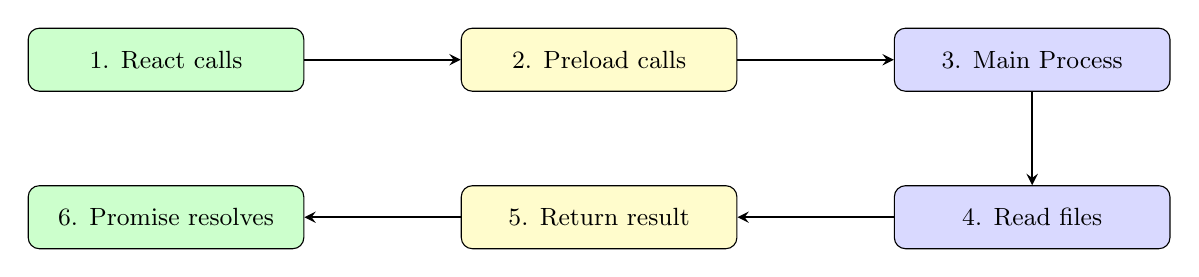
\begin{tikzpicture}[
    stepbox/.style={draw, rounded corners, fill=blue!10, minimum width=3.5cm, minimum height=0.8cm, align=center, font=\small},
    arrow/.style={->, thick, >=stealth}
]
    \node[stepbox, fill=green!20] (s1) at (0, 0) {1. React calls};
    \node[stepbox, fill=yellow!20] (s2) at (5.5, 0) {2. Preload calls};
    \node[stepbox, fill=blue!15] (s3) at (11, 0) {3. Main Process};
    
    \node[stepbox, fill=blue!15] (s4) at (11, -2) {4. Read files};
    \node[stepbox, fill=yellow!20] (s5) at (5.5, -2) {5. Return result};
    \node[stepbox, fill=green!20] (s6) at (0, -2) {6. Promise resolves};
    
    \draw[arrow] (s1) -- (s2);
    \draw[arrow] (s2) -- (s3);
    \draw[arrow] (s3) -- (s4);
    \draw[arrow] (s4) -- (s5);
    \draw[arrow] (s5) -- (s6);
\end{tikzpicture}
\caption{Complete IPC Request Lifecycle}
\end{figure}

\section{invoke vs send: When to Use Which}

\begin{table}[ht!]
\centering
\begin{tabular}{@{}p{4cm}p{5cm}p{5cm}@{}}
\toprule
\textbf{Method} & \textbf{ipcRenderer.invoke()} & \textbf{ipcRenderer.send()} \\
\midrule
\textbf{Pattern} & Request $\rightarrow$ Response & Fire \& Forget \\
\textbf{Returns} & Promise (awaitable) & Nothing \\
\textbf{Use When} & You need data back & Just notifying Main \\
\textbf{Example} & Get list of songs & Notify playback started \\
\textbf{Handler} & \inlinecode{ipcMain.handle()} & \inlinecode{ipcMain.on()} \\
\bottomrule
\end{tabular}
\caption{invoke vs send Comparison}
\end{table}

\begin{lstlisting}[language=TypeScript, title=Examples in preload.ts]
// INVOKE: Need response (which folder did user pick?)
selectMusicFolder: () => ipcRenderer.invoke('select-music-folder'),

// SEND: Fire-and-forget (just telling Main the state changed)
sendPlaybackState: (isPlaying) => {
  ipcRenderer.send('playback-state-changed', isPlaying);
},
\end{lstlisting}

\section{Listening for Events from Main Process}

Sometimes the Main Process needs to \textbf{push data to the Renderer} (e.g., download progress).

\begin{lstlisting}[language=TypeScript, title=preload.ts]
// Register a listener that calls a callback when Main sends an event
onDownloadProgress: (callback) => {
  const handler = (_event, progress) => callback(progress);
  ipcRenderer.on('download-progress', handler);
  // Return cleanup function
  return () => ipcRenderer.removeListener('download-progress', handler);
},
\end{lstlisting}

\begin{lstlisting}[language=TypeScript, title=youtubeHandlers.ts (Main Process)]
// Main Process sends progress updates to Renderer
window.webContents.send('download-progress', {
  percentage: 50,
  speed: '1.2 MB/s',
  eta: '00:15'
});
\end{lstlisting}

\section{IPC Channel Naming Convention}

All channels use \textbf{kebab-case} with descriptive names:

\begin{tabular}{@{}p{5cm}p{9cm}@{}}
\inlinecode{scan-music-folder} & Action on noun \\
\inlinecode{download-progress} & Event type \\
\inlinecode{cache-get-file-status} & Module-action-target \\
\inlinecode{playlist-add-songs} & Module-action-target \\
\end{tabular}

%%%%%%%%%%%%%%%%%%%%%%%%%%%%%%%%%%%%%%%%%%%%%%%%%%%%%%%%%%%%%%%%%%%%%%%%%%%%%%%
% DETAILED IPC CALL TYPES
%%%%%%%%%%%%%%%%%%%%%%%%%%%%%%%%%%%%%%%%%%%%%%%%%%%%%%%%%%%%%%%%%%%%%%%%%%%%%%%
\section{IPC Call Types: Complete Reference}

This section covers \textbf{every type of IPC call} used in Electron with real examples from this codebase.

\subsection{Type 1: Async Request/Response (invoke/handle)}

\textbf{The most common pattern.} Renderer asks a question, Main answers.

\begin{figure}[ht!]
\centering
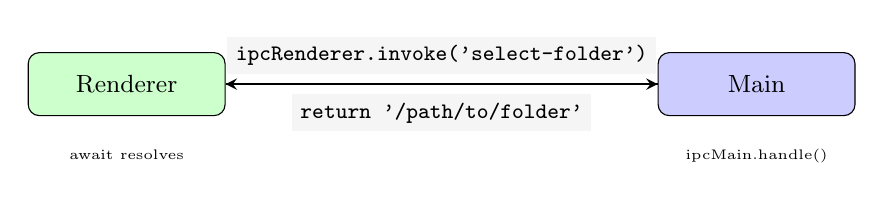
\begin{tikzpicture}[
    box/.style={draw, rounded corners, minimum width=2.5cm, minimum height=0.8cm, align=center, font=\small},
    arrow/.style={->, thick, >=stealth}
]
    \node[box, fill=green!20] (r1) at (0, 0) {Renderer};
    \node[box, fill=blue!20] (m1) at (8, 0) {Main};
    
    \draw[arrow] (r1) -- node[above, font=\footnotesize] {\inlinecode{ipcRenderer.invoke('select-folder')}} (m1);
    \draw[arrow, dashed] (m1) -- node[below, font=\footnotesize] {\inlinecode{return '/path/to/folder'}} (r1);
    
    \node[font=\tiny, below=0.3cm of r1] {await resolves};
    \node[font=\tiny, below=0.3cm of m1] {ipcMain.handle()};
\end{tikzpicture}
\caption{Async Request/Response Pattern}
\end{figure}

\textbf{Preload (Renderer Side):}
\begin{lstlisting}[language=TypeScript]
// Returns a Promise that resolves with the result
selectMusicFolder: () => ipcRenderer.invoke('select-music-folder'),

// Usage in React:
const folder = await window.electronAPI.selectMusicFolder();
// folder = '/Users/me/Music' or null
\end{lstlisting}

\textbf{Handler (Main Side):}
\begin{lstlisting}[language=TypeScript]
ipcMain.handle('select-music-folder', async () => {
  const result = await dialog.showOpenDialog({
    properties: ['openDirectory'],
    title: 'Select Music Folder',
  });
  if (!result.canceled && result.filePaths.length > 0) {
    return result.filePaths[0];  // <-- This becomes the Promise result
  }
  return null;
});
\end{lstlisting}

\begin{tipbox}
\textbf{Key Points:}
\begin{itemize}
    \item \inlinecode{invoke()} returns a \textbf{Promise} --- use \inlinecode{await} or \inlinecode{.then()}
    \item \inlinecode{handle()} can be \textbf{async} --- use \inlinecode{async/await} inside
    \item Whatever you \textbf{return} in \inlinecode{handle()} becomes the Promise result
    \item If handler throws, Promise \textbf{rejects} with the error
\end{itemize}
\end{tipbox}

\subsection{Type 2: Fire-and-Forget (send/on)}

\textbf{No response needed.} Renderer notifies Main about something.

\begin{figure}[ht!]
\centering
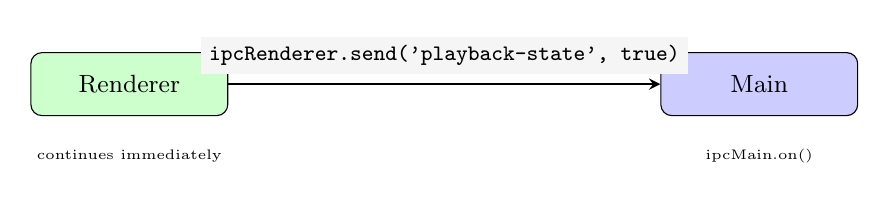
\begin{tikzpicture}[
    box/.style={draw, rounded corners, minimum width=2.5cm, minimum height=0.8cm, align=center, font=\small},
    arrow/.style={->, thick, >=stealth}
]
    \node[box, fill=green!20] (r1) at (0, 0) {Renderer};
    \node[box, fill=blue!20] (m1) at (8, 0) {Main};
    
    \draw[arrow] (r1) -- node[above, font=\footnotesize] {\inlinecode{ipcRenderer.send('playback-state', true)}} (m1);
    
    \node[font=\tiny, below=0.3cm of r1] {continues immediately};
    \node[font=\tiny, below=0.3cm of m1] {ipcMain.on()};
\end{tikzpicture}
\caption{Fire-and-Forget Pattern}
\end{figure}

\textbf{Preload:}
\begin{lstlisting}[language=TypeScript]
// No await needed - just fire and continue
sendPlaybackState: (isPlaying: boolean) => {
  ipcRenderer.send('playback-state-changed', isPlaying);
},

// Window controls - no response expected
minimizeWindow: () => ipcRenderer.send('window-minimize'),
maximizeWindow: () => ipcRenderer.send('window-maximize'),
closeWindow: () => ipcRenderer.send('window-close'),
\end{lstlisting}

\textbf{Handler:}
\begin{lstlisting}[language=TypeScript]
// Use .on() instead of .handle() for fire-and-forget
ipcMain.on('playback-state-changed', (_event, isPlaying: boolean) => {
  // Update tray menu label
  updatePlaybackState(isPlaying);
  // No return value - nothing to send back
});

ipcMain.on('window-minimize', () => {
  BrowserWindow.getFocusedWindow()?.minimize();
});
\end{lstlisting}

\begin{notebox}
\textbf{When to use Fire-and-Forget:}
\begin{itemize}
    \item Window controls (minimize, maximize, close)
    \item Notifying Main about state changes (playback started/stopped)
    \item Logging or analytics events
    \item Any case where you don't need confirmation
\end{itemize}
\end{notebox}

\subsection{Type 3: Event Listener (Main $\rightarrow$ Renderer Push)}

\textbf{Main Process pushes updates to Renderer.} Used for progress updates, real-time events.

\begin{figure}[ht!]
\centering
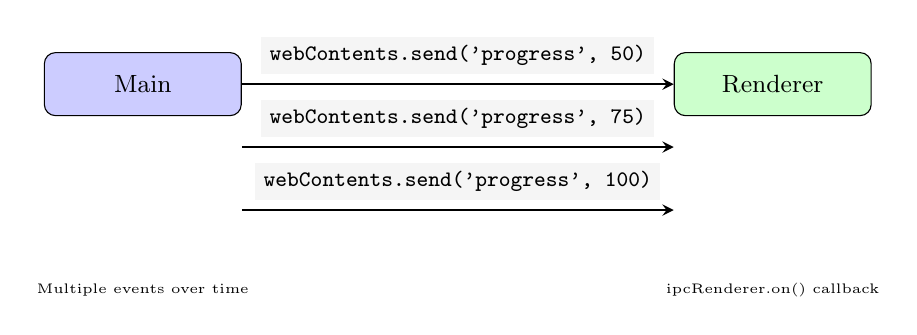
\begin{tikzpicture}[
    box/.style={draw, rounded corners, minimum width=2.5cm, minimum height=0.8cm, align=center, font=\small},
    arrow/.style={->, thick, >=stealth}
]
    \node[box, fill=blue!20] (m1) at (0, 0) {Main};
    \node[box, fill=green!20] (r1) at (8, 0) {Renderer};
    
    \draw[arrow] (m1) -- node[above, font=\footnotesize] {\inlinecode{webContents.send('progress', 50)}} (r1);
    \draw[arrow] ([yshift=-0.8cm]m1.east) -- node[above, font=\footnotesize] {\inlinecode{webContents.send('progress', 75)}} ([yshift=-0.8cm]r1.west);
    \draw[arrow] ([yshift=-1.6cm]m1.east) -- node[above, font=\footnotesize] {\inlinecode{webContents.send('progress', 100)}} ([yshift=-1.6cm]r1.west);
    
    \node[font=\tiny, below=2cm of m1] {Multiple events over time};
    \node[font=\tiny, below=2cm of r1] {ipcRenderer.on() callback};
\end{tikzpicture}
\caption{Event Listener Pattern (Main Pushes to Renderer)}
\end{figure}

\textbf{Preload (Register Listener):}
\begin{lstlisting}[language=TypeScript]
// Register a callback that fires whenever Main sends an event
onDownloadProgress: (callback: (progress: any) => void) => {
  const handler = (_event: any, progress: any) => callback(progress);
  ipcRenderer.on('download-progress', handler);
  
  // Return cleanup function (important for React useEffect!)
  return () => {
    ipcRenderer.removeListener('download-progress', handler);
  };
},
\end{lstlisting}

\textbf{React Component:}
\begin{lstlisting}[language=TypeScript]
useEffect(() => {
  // Subscribe to progress events
  const cleanup = window.electronAPI.onDownloadProgress((progress) => {
    setProgress(progress.percentage);
    setSpeed(progress.speed);
  });
  
  // Unsubscribe when component unmounts
  return cleanup;
}, []);
\end{lstlisting}

\textbf{Main Process (Send Events):}
\begin{lstlisting}[language=TypeScript]
// Inside youtubeHandlers.ts
ytDlpProcess.stdout.on('data', (data) => {
  const progress = parseProgress(data);
  // Push progress to Renderer
  window.webContents.send('download-progress', {
    percentage: progress.percent,
    speed: progress.speed,
    eta: progress.eta
  });
});
\end{lstlisting}

\begin{tipbox}
\textbf{Cleanup is Critical!}

Always return a cleanup function and call it when the React component unmounts. Otherwise:
\begin{itemize}
    \item Memory leaks (handlers pile up)
    \item Stale callbacks (old components still receiving events)
    \item Multiple handlers for same event
\end{itemize}
\end{tipbox}

\subsection{Type 4: Bidirectional Streaming}

\textbf{Continuous back-and-forth.} Used for batch operations with progress.

\begin{figure}[ht!]
\centering
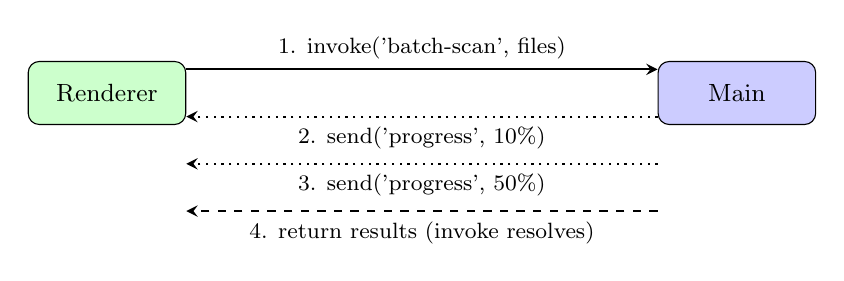
\begin{tikzpicture}[
    box/.style={draw, rounded corners, minimum width=2cm, minimum height=0.8cm, align=center, font=\small},
    arrow/.style={->, thick, >=stealth}
]
    \node[box, fill=green!20] (r) at (0, 0) {Renderer};
    \node[box, fill=blue!20] (m) at (8, 0) {Main};
    
    \draw[arrow] ([yshift=0.3cm]r.east) -- node[above, font=\footnotesize] {1. invoke('batch-scan', files)} ([yshift=0.3cm]m.west);
    \draw[arrow, dotted] ([yshift=-0.3cm]m.west) -- node[below, font=\footnotesize] {2. send('progress', 10\%)} ([yshift=-0.3cm]r.east);
    \draw[arrow, dotted] ([yshift=-0.9cm]m.west) -- node[below, font=\footnotesize] {3. send('progress', 50\%)} ([yshift=-0.9cm]r.east);
    \draw[arrow, dashed] ([yshift=-1.5cm]m.west) -- node[below, font=\footnotesize] {4. return results (invoke resolves)} ([yshift=-1.5cm]r.east);
\end{tikzpicture}
\caption{Bidirectional: Request + Progress Events + Final Response}
\end{figure}

\textbf{This codebase example (Fingerprint Batch):}
\begin{lstlisting}[language=TypeScript]
// Preload - Two separate registrations
generateFingerprintsBatch: (filePaths: string[]) =>
  ipcRenderer.invoke('generate-fingerprints-batch', filePaths),

onFingerprintBatchProgress: (callback) => {
  const handler = (_event, progress) => callback(progress);
  ipcRenderer.on('fingerprint-batch-progress', handler);
  return () => ipcRenderer.removeListener('fingerprint-batch-progress', handler);
},
\end{lstlisting}

\begin{lstlisting}[language=TypeScript]
// React usage - both together
useEffect(() => {
  const cleanup = window.electronAPI.onFingerprintBatchProgress((p) => {
    setProgress(p.percentage);
  });
  return cleanup;
}, []);

const handleScan = async () => {
  // This call triggers progress events while running
  const results = await window.electronAPI.generateFingerprintsBatch(files);
  // results contains final data after all progress events
};
\end{lstlisting}

\subsection{Summary: All IPC Patterns}

\begin{table}[ht!]
\centering
\small
\begin{tabular}{@{}p{2.5cm}p{3cm}p{3cm}p{2.5cm}p{3cm}@{}}
\toprule
\textbf{Pattern} & \textbf{Renderer API} & \textbf{Main API} & \textbf{Returns} & \textbf{Use Case} \\
\midrule
Async Request & \inlinecode{invoke()} & \inlinecode{handle()} & Promise & Get data \\
Fire-and-Forget & \inlinecode{send()} & \inlinecode{on()} & Nothing & Notify state \\
Event Listener & \inlinecode{on()} & \inlinecode{send()} & Callback & Progress \\
Bidirectional & Both & Both & Both & Batch ops \\
\bottomrule
\end{tabular}
\caption{IPC Pattern Summary}
\end{table}

\subsection{Error Handling in IPC}

\textbf{Errors in \inlinecode{handle()} propagate to Renderer:}

\begin{lstlisting}[language=TypeScript]
// Main Process
ipcMain.handle('risky-operation', async () => {
  throw new Error('Something went wrong');
});

// Renderer - error is caught!
try {
  await window.electronAPI.riskyOperation();
} catch (error) {
  console.error('IPC error:', error.message);
  // Shows: "Something went wrong"
}
\end{lstlisting}

\textbf{Best practice - return error objects:}
\begin{lstlisting}[language=TypeScript]
// Main Process
ipcMain.handle('write-metadata', async (_event, filePath, metadata) => {
  try {
    await writeMetadata(filePath, metadata);
    return { success: true };
  } catch (error) {
    return { success: false, error: error.message };
  }
});

// Renderer
const result = await window.electronAPI.writeMetadata(path, meta);
if (!result.success) {
  showToast('error', result.error);
}
\end{lstlisting}

\section{Handler Module Registration}

Handlers are organized into \textbf{modular files} for better maintainability.

\begin{figure}[ht!]
\centering
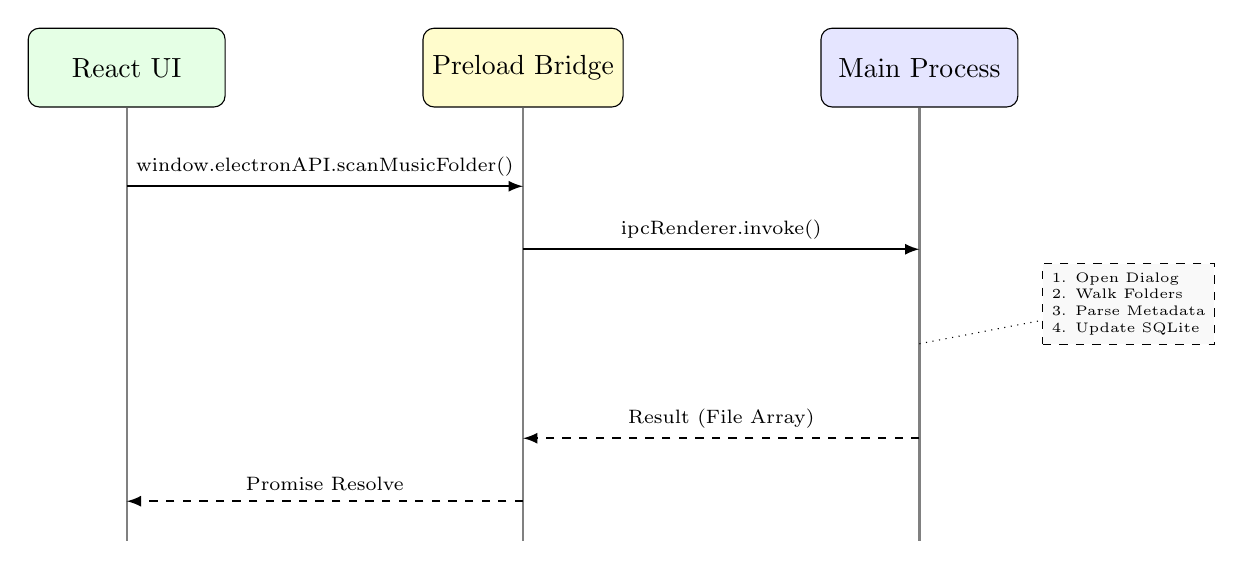
\begin{tikzpicture}[
    node distance=2.5cm,
    actor/.style={draw, rectangle, minimum width=2.5cm, minimum height=1cm, fill=white, rounded corners},
    line/.style={draw, -latex, thick}
]
    % Vertical Lifelines
    \node[actor, fill=green!10] (react) {React UI};
    \node[actor, fill=yellow!20, right=of react] (preload) {Preload Bridge};
    \node[actor, fill=blue!10, right=of preload] (main) {Main Process};
    
    \draw[thick, gray] (react.south) -- +(0,-5.5);
    \draw[thick, gray] (preload.south) -- +(0,-5.5);
    \draw[thick, gray] (main.south) -- +(0,-5.5);
    
    % Messages
    \draw[line] ([yshift=-1cm]react.south) -- node[above, font=\scriptsize] {window.electronAPI.scanMusicFolder()} ([yshift=-1cm]preload.south);
    \draw[line] ([yshift=-1.8cm]preload.south) -- node[above, font=\scriptsize] {ipcRenderer.invoke()} ([yshift=-1.8cm]main.south);
    
    \node[draw, fill=gray!5, font=\tiny, right=0.3cm of main, yshift=-3cm, align=left, dashed] (work) {
        1. Open Dialog\\
        2. Walk Folders\\
        3. Parse Metadata\\
        4. Update SQLite
    };
    \draw[dotted] ([yshift=-3cm]main.south) -- (work);
    
    \draw[line, dashed] ([yshift=-4.2cm]main.south) -- node[above, font=\scriptsize] {Result (File Array)} ([yshift=-4.2cm]preload.south);
    \draw[line, dashed] ([yshift=-5.0cm]preload.south) -- node[above, font=\scriptsize] {Promise Resolve} ([yshift=-5.0cm]react.south);
\end{tikzpicture}
\caption{IPC Request/Response Sequence Diagram}
\label{fig:ipc_sequence}
\end{figure}

\section{All IPC Endpoints}

\begin{longtable}{@{}p{3cm}p{4.5cm}p{1.5cm}p{5.5cm}@{}}
\toprule
\textbf{Module} & \textbf{Handler} & \textbf{Type} & \textbf{Purpose} \\
\midrule
\endhead

musicHandlers & \inlinecode{scan-music-folder} & invoke & Scan directory for music files \\
& \inlinecode{select-music-folder} & invoke & Open folder selection dialog \\
& \inlinecode{read-single-file-metadata} & invoke & Read metadata for a single file \\
& \inlinecode{write-cover-art} & invoke & Embed cover art in audio file \\
& \inlinecode{write-metadata} & invoke & Write all metadata to audio file \\
\addlinespace

apiHandlers & \inlinecode{lookup-acoustid} & invoke & Query AcoustID API \\
& \inlinecode{lookup-musicbrainz} & invoke & Query MusicBrainz API \\
& \inlinecode{download-image} & invoke & Download cover art image \\
& \inlinecode{download-image-with-fallback} & invoke & Download cover art with fallback URLs \\
\addlinespace

youtubeHandlers & \inlinecode{download-youtube} & invoke & Download audio from YouTube \\
& \inlinecode{get-binary-statuses} & invoke & Get status of yt-dlp binary \\
\addlinespace

systemHandlers & \inlinecode{window-minimize} & on & Minimize window \\
& \inlinecode{window-maximize} & on & Toggle maximize/restore \\
& \inlinecode{window-close} & on & Close window \\
& \inlinecode{get-settings} & invoke & Get stored settings from disk \\
& \inlinecode{save-settings} & invoke & Save settings to disk \\
\addlinespace

cacheHandlers & \inlinecode{cache-get-file-status} & invoke & Get scan status for a file \\
& \inlinecode{cache-mark-file-scanned} & invoke & Record scan result in database \\
& \inlinecode{cache-get-batch-status} & invoke & Get status for multiple files \\
& \inlinecode{cache-get-statistics} & invoke & Get total/tagged/untagged counts \\
\addlinespace

fingerprintHandlers & \inlinecode{generate-fingerprint} & invoke & Generate AcoustID fingerprint \\
& \inlinecode{fingerprint-check-ready} & invoke & Check if fpcalc is installed \\
\addlinespace

playlistHandlers & \inlinecode{playlist-create} & invoke & Create a new playlist \\
& \inlinecode{playlist-delete} & invoke & Delete a playlist \\
& \inlinecode{playlist-get-all} & invoke & Get all playlists \\
& \inlinecode{playlist-add-songs} & invoke & Add songs to a playlist \\
& \inlinecode{playlist-remove-song} & invoke & Remove a song from a playlist \\
\bottomrule
\caption{All IPC Endpoints}
\end{longtable}

% Song Identification User Journey
\begin{figure}[ht!]
\centering
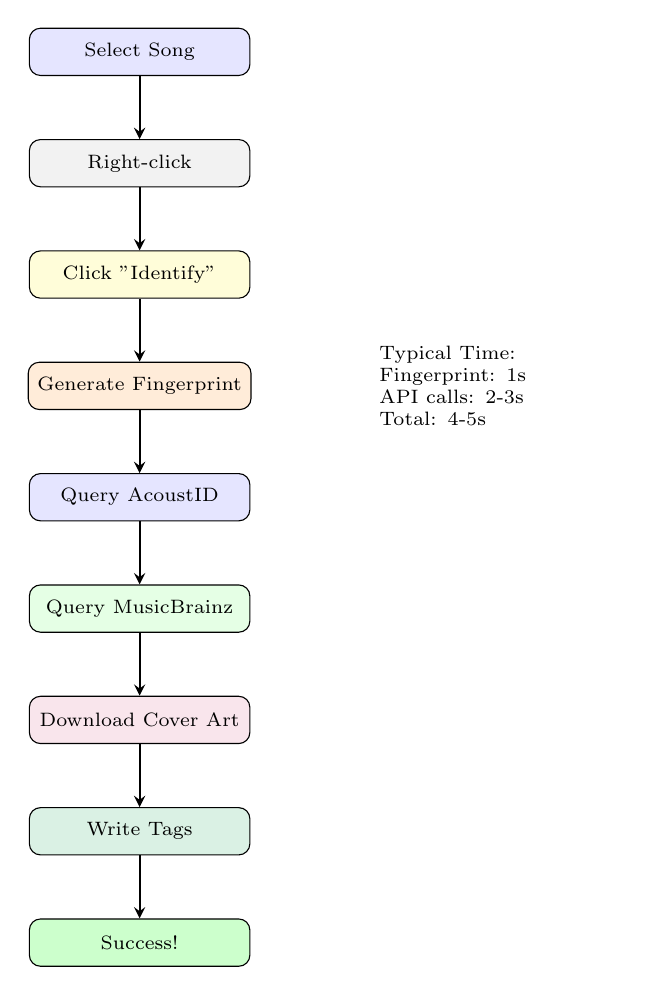
\begin{tikzpicture}[
    node distance=0.8cm,
    box/.style={draw, rounded corners, minimum width=2.8cm, minimum height=0.6cm, align=center, font=\scriptsize},
    arrow/.style={->, thick, >=stealth}
]
    \node[box, fill=blue!10] (select) {Select Song};
    \node[box, fill=gray!10, below=of select] (rightclick) {Right-click};
    \node[box, fill=yellow!15, below=of rightclick] (identify) {Click ''Identify''};
    \node[box, fill=orange!15, below=of identify] (fingerprint) {Generate Fingerprint};
    \node[box, fill=blue!10, below=of fingerprint] (acoustid) {Query AcoustID};
    \node[box, fill=green!10, below=of acoustid] (musicbrainz) {Query MusicBrainz};
    \node[box, fill=purple!10, below=of musicbrainz] (cover) {Download Cover Art};
    \node[box, fill=successcolor!20, below=of cover] (write) {Write Tags};
    \node[box, fill=green!20, below=of write] (success) {Success!};
    
    \draw[arrow] (select) -- (rightclick);
    \draw[arrow] (rightclick) -- (identify);
    \draw[arrow] (identify) -- (fingerprint);
    \draw[arrow] (fingerprint) -- (acoustid);
    \draw[arrow] (acoustid) -- (musicbrainz);
    \draw[arrow] (musicbrainz) -- (cover);
    \draw[arrow] (cover) -- (write);
    \draw[arrow] (write) -- (success);
    
    \node[right=1.5cm of fingerprint, text width=3cm, font=\scriptsize, align=left] {Typical Time:\\Fingerprint: 1s\\API calls: 2-3s\\Total: 4-5s};
\end{tikzpicture}
\caption{Song Identification User Journey}
\label{fig:song_id_journey}
\end{figure}

% YouTube Download User Flow
\begin{figure}[ht!]
\centering
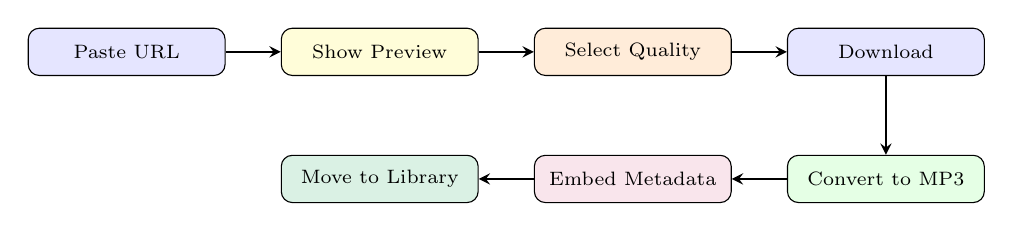
\begin{tikzpicture}[
    node distance=0.7cm,
    box/.style={draw, rounded corners, minimum width=2.5cm, minimum height=0.6cm, align=center, font=\scriptsize},
    arrow/.style={->, thick, >=stealth}
]
    \node[box, fill=blue!10] (paste) {Paste URL};
    \node[box, fill=yellow!15, right=of paste] (preview) {Show Preview};
    \node[box, fill=orange!15, right=of preview] (quality) {Select Quality};
    \node[box, fill=blue!10, right=of quality] (download) {Download};
    \node[box, fill=green!10, below=1cm of download] (convert) {Convert to MP3};
    \node[box, fill=purple!10, left=of convert] (embed) {Embed Metadata};
    \node[box, fill=successcolor!20, left=of embed] (move) {Move to Library};
    
    \draw[arrow] (paste) -- (preview);
    \draw[arrow] (preview) -- (quality);
    \draw[arrow] (quality) -- (download);
    \draw[arrow] (download) -- (convert);
    \draw[arrow] (convert) -- (embed);
    \draw[arrow] (embed) -- (move);
\end{tikzpicture}
\caption{YouTube Download User Flow}
\label{fig:youtube_user_flow}
\end{figure}

% Settings Persistence Flow
\begin{figure}[ht!]
\centering
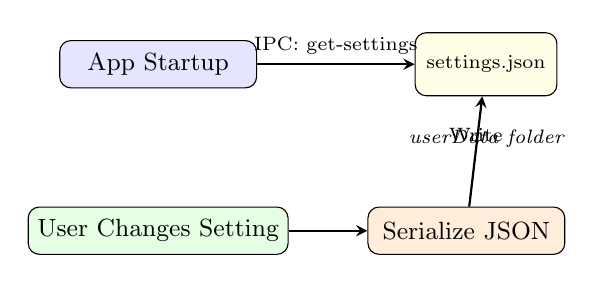
\begin{tikzpicture}[
    node distance=1cm,
    box/.style={draw, rounded corners, minimum width=2.5cm, minimum height=0.6cm, align=center, font=\small},
    storage/.style={draw, rounded corners, minimum width=1.8cm, minimum height=0.8cm, fill=yellow!10, font=\scriptsize, align=center},
    arrow/.style={->, thick, >=stealth}
]
    \node[box, fill=blue!10] (startup) {App Startup};
    \node[storage, right=2cm of startup] (json) {settings.json};
    \node[box, fill=green!10, below=1.5cm of startup] (user) {User Changes Setting};
    \node[box, fill=orange!15, right=of user] (serialize) {Serialize JSON};
    
    \draw[arrow] (startup) -- node[above, font=\scriptsize] {IPC: get-settings} (json);
    \draw[arrow] (user) -- (serialize);
    \draw[arrow] (serialize) -- node[above, font=\scriptsize] {Write} (json);
    
    \node[below=0.3cm of json, font=\scriptsize\itshape] {userData folder};
\end{tikzpicture}
\caption{Settings Persistence Flow}
\label{fig:settings_flow}
\end{figure}

% Playlist Creation Flow
\begin{figure}[ht!]
\centering
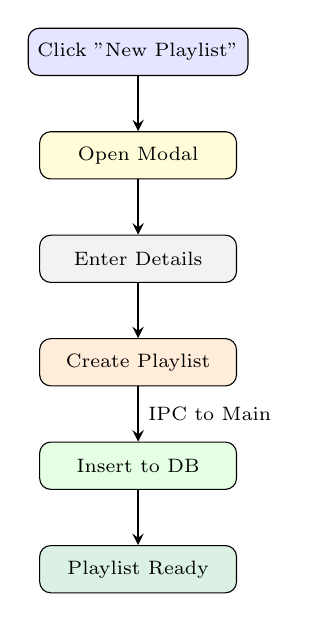
\begin{tikzpicture}[
    node distance=0.7cm,
    box/.style={draw, rounded corners, minimum width=2.5cm, minimum height=0.6cm, align=center, font=\scriptsize},
    arrow/.style={->, thick, >=stealth}
]
    \node[box, fill=blue!10] (click) {Click ''New Playlist''};
    \node[box, fill=yellow!15, below=of click] (modal) {Open Modal};
    \node[box, fill=gray!10, below=of modal] (enter) {Enter Details};
    \node[box, fill=orange!15, below=of enter] (create) {Create Playlist};
    \node[box, fill=green!10, below=of create] (insert) {Insert to DB};
    \node[box, fill=successcolor!20, below=of insert] (ready) {Playlist Ready};
    
    \draw[arrow] (click) -- (modal);
    \draw[arrow] (modal) -- (enter);
    \draw[arrow] (enter) -- (create);
    \draw[arrow] (create) -- node[right, font=\scriptsize] {IPC to Main} (insert);
    \draw[arrow] (insert) -- (ready);
\end{tikzpicture}
\caption{Playlist Creation Flow}
\label{fig:playlist_creation}
\end{figure}

% Lyrics Generation Workflow
\begin{figure}[ht!]
\centering
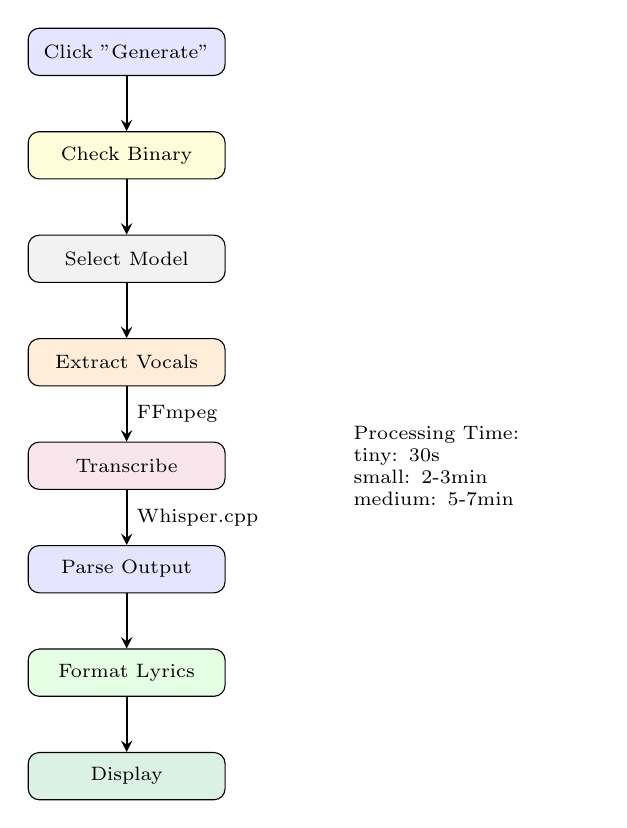
\begin{tikzpicture}[
    node distance=0.7cm,
    box/.style={draw, rounded corners, minimum width=2.5cm, minimum height=0.6cm, align=center, font=\scriptsize},
    arrow/.style={->, thick, >=stealth}
]
    \node[box, fill=blue!10] (click) {Click ''Generate''};
    \node[box, fill=yellow!15, below=of click] (check) {Check Binary};
    \node[box, fill=gray!10, below=of check] (model) {Select Model};
    \node[box, fill=orange!15, below=of model] (extract) {Extract Vocals};
    \node[box, fill=purple!10, below=of extract] (transcribe) {Transcribe};
    \node[box, fill=blue!10, below=of transcribe] (parse) {Parse Output};
    \node[box, fill=green!10, below=of parse] (format) {Format Lyrics};
    \node[box, fill=successcolor!20, below=of format] (display) {Display};
    
    \draw[arrow] (click) -- (check);
    \draw[arrow] (check) -- (model);
    \draw[arrow] (model) -- (extract);
    \draw[arrow] (extract) -- node[right, font=\scriptsize] {FFmpeg} (transcribe);
    \draw[arrow] (transcribe) -- node[right, font=\scriptsize] {Whisper.cpp} (parse);
    \draw[arrow] (parse) -- (format);
    \draw[arrow] (format) -- (display);
    
    \node[right=1.5cm of transcribe, text width=3cm, font=\scriptsize, align=left] {Processing Time:\\tiny: 30s\\small: 2-3min\\medium: 5-7min};
\end{tikzpicture}
\caption{Lyrics Generation Workflow}
\label{fig:lyrics_workflow}
\end{figure}

% Album Art Processing Flow
\begin{figure}[ht!]
\centering
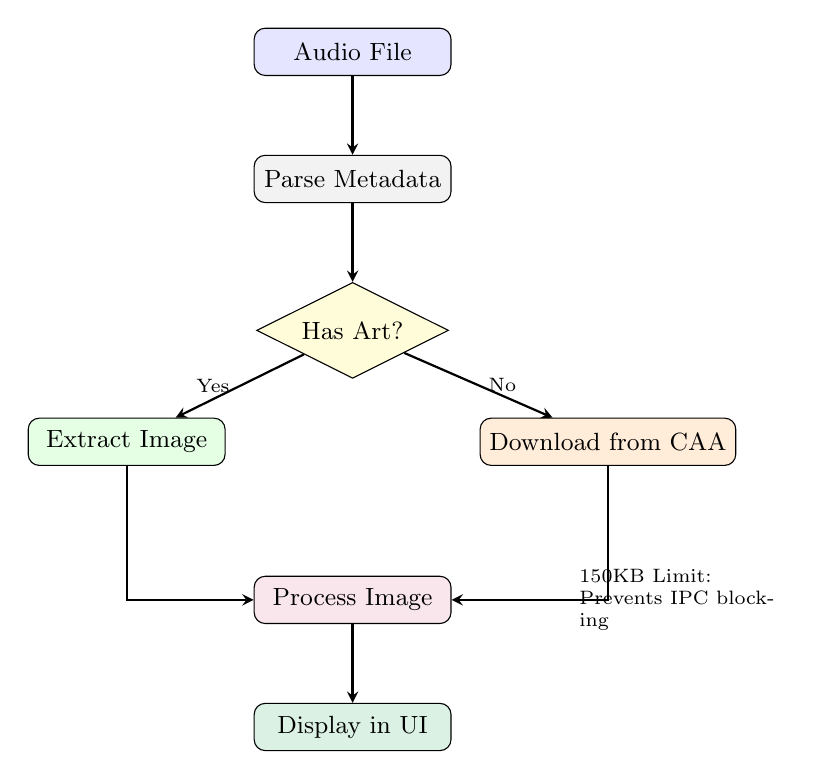
\begin{tikzpicture}[
    node distance=1cm,
    box/.style={draw, rounded corners, minimum width=2.5cm, minimum height=0.6cm, align=center, font=\small},
    decision/.style={draw, diamond, aspect=2, fill=yellow!15, font=\small},
    arrow/.style={->, thick, >=stealth}
]
    \node[box, fill=blue!10] (file) {Audio File};
    \node[box, fill=gray!10, below=of file] (parse) {Parse Metadata};
    \node[decision, below=of parse] (has) {Has Art?};
    \node[box, fill=green!10, below left=0.8cm and 1cm of has] (extract) {Extract Image};
    \node[box, fill=orange!15, below right=0.8cm and 1cm of has] (download) {Download from CAA};
    \node[box, fill=purple!10, below=2.5cm of has] (process) {Process Image};
    \node[box, fill=successcolor!20, below=of process] (display) {Display in UI};
    
    \draw[arrow] (file) -- (parse);
    \draw[arrow] (parse) -- (has);
    \draw[arrow] (has) -- node[left, font=\scriptsize] {Yes} (extract);
    \draw[arrow] (has) -- node[right, font=\scriptsize] {No} (download);
    \draw[arrow] (extract) |- (process);
    \draw[arrow] (download) |- (process);
    \draw[arrow] (process) -- (display);
    
    \node[right=1.5cm of process, font=\scriptsize, text width=2.5cm, align=left] {150KB Limit:\\Prevents IPC blocking};
\end{tikzpicture}
\caption{Album Art Extraction and Embedding}
\label{fig:album_art_flow}
\end{figure}

% IPC Channels Map
\begin{figure}[ht!]
\centering
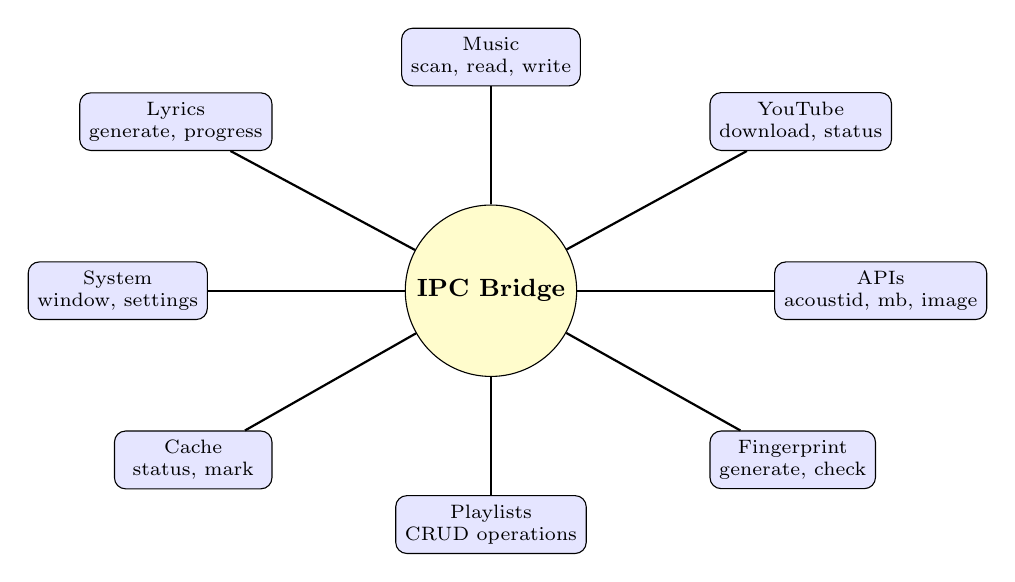
\begin{tikzpicture}[
    node distance=0.3cm,
    hub/.style={draw, circle, fill=yellow!20, minimum size=1.5cm, font=\small\bfseries, align=center},
    module/.style={draw, rounded corners, fill=blue!10, minimum width=2cm, minimum height=0.5cm, font=\scriptsize, align=center}
]
    \node[hub] (bridge) {IPC Bridge};
    
    \node[module, above=1.5cm of bridge] (music) {Music\\scan, read, write};
    \node[module, above right=1cm and 2cm of bridge] (youtube) {YouTube\\download, status};
    \node[module, right=2.5cm of bridge] (apis) {APIs\\acoustid, mb, image};
    \node[module, below right=1cm and 2cm of bridge] (fingerprint) {Fingerprint\\generate, check};
    \node[module, below=1.5cm of bridge] (playlists) {Playlists\\CRUD operations};
    \node[module, below left=1cm and 2cm of bridge] (cache) {Cache\\status, mark};
    \node[module, left=2.5cm of bridge] (system) {System\\window, settings};
    \node[module, above left=1cm and 2cm of bridge] (lyrics) {Lyrics\\generate, progress};
    
    \draw[thick] (bridge) -- (music);
    \draw[thick] (bridge) -- (youtube);
    \draw[thick] (bridge) -- (apis);
    \draw[thick] (bridge) -- (fingerprint);
    \draw[thick] (bridge) -- (playlists);
    \draw[thick] (bridge) -- (cache);
    \draw[thick] (bridge) -- (system);
    \draw[thick] (bridge) -- (lyrics);
\end{tikzpicture}
\caption{IPC Channels Map: Modular Handler Organization}
\label{fig:ipc_channels_map}
\end{figure}

%%%%%%%%%%%%%%%%%%%%%%%%%%%%%%%%%%%%%%%%%%%%%%%%%%%%%%%%%%%%%%%%%%%%%%%%%%%%%%%
% CHAPTER 5: EXTERNAL API INTEGRATION
%%%%%%%%%%%%%%%%%%%%%%%%%%%%%%%%%%%%%%%%%%%%%%%%%%%%%%%%%%%%%%%%%%%%%%%%%%%%%%%
\chapter{External API Integration}
\label{ch:api}

\begin{tipbox}
\textbf{Real-World Analogy: Song Detective Work}

Imagine you find an unmarked music CD. To identify the songs, you'd:
\begin{enumerate}
    \item \textbf{Listen to it} (Generate audio fingerprint)
    \item \textbf{Ask a music expert} "What song has this melody?" (AcoustID)
    \item \textbf{Look it up in a music encyclopedia} (MusicBrainz)
    \item \textbf{Find the album cover} (Cover Art Archive)
    \item \textbf{Label the CD} (Write metadata to file)
\end{enumerate}
This is exactly what the app does automatically!
\end{tipbox}

\section{Complete Song Identification Workflow}

\begin{figure}[ht!]
\centering
\begin{tikzpicture}[
    node distance=0.7cm,
    startbox/.style={rectangle, draw=blue!70, fill=blue!15, thick, minimum width=4cm, minimum height=0.8cm, text width=3.8cm, align=center, font=\small\bfseries},
    processbox/.style={rectangle, draw=green!70, fill=green!15, thick, minimum width=4cm, minimum height=0.8cm, text width=3.8cm, align=center, font=\small},
    apibox/.style={ellipse, draw=orange!70, fill=orange!15, thick, minimum width=3.5cm, minimum height=1cm, align=center, font=\small\bfseries},
    checkdiamond/.style={diamond, draw=red!70, fill=red!15, thick, minimum width=2.5cm, minimum height=1.2cm, text width=2.2cm, align=center, font=\tiny\bfseries},
    successbox/.style={rectangle, draw=purple!70, fill=purple!15, thick, minimum width=4cm, minimum height=0.8cm, text width=3.8cm, align=center, font=\small},
    errorbox/.style={rectangle, draw=red!70, fill=red!15, thick, minimum width=3cm, minimum height=0.7cm, text width=2.8cm, align=center, font=\small},
]
    % Start
    \node[startbox] (start) at (0,0) {1. Unknown Audio File\\mystery\_song.mp3};
    
    % Generate fingerprint
    \node[processbox, below=of start] (fpcalc) {2. Generate Fingerprint\\Run fpcalc binary\\(19ms avg)};
    
    % Check fingerprint
    \node[checkdiamond, below=1cm of fpcalc] (fpcheck) {Finger-\\print\\OK?};
    
    % Fingerprint error
    \node[errorbox, left=2cm of fpcheck] (fperror) {ERROR:\\Audio corrupt};
    
    % AcoustID lookup
    \node[apibox, below=1.2cm of fpcheck] (acoustid) {3. AcoustID API\\``What song is this?''};
    
    % Confidence check
    \node[checkdiamond, below=1cm of acoustid] (confcheck) {Confidence\\>70\%?};
    
    % Low confidence
    \node[errorbox, left=2cm of confcheck] (noconf) {No Match\\(confidence too low)};
    
    % Got MBID
    \node[processbox, below=1.2cm of confcheck] (mbid) {4. Got MBID\\(MusicBrainz ID)};
    
    % MusicBrainz lookup
    \node[apibox, below=of mbid] (mb) {5. MusicBrainz API\\Get full metadata};
    
    % Cover art lookup
    \node[apibox, below=of mb] (caa) {6. Cover Art Archive\\Download album art};
    
    % Write to file
    \node[successbox, below=of caa] (write) {7. Write to File\\taglib-wasm embeds\\title, artist, album, art};
    
    % Success
    \node[startbox, fill=green!20, below=of write] (success) {✓ Song Identified!\\Beautiful metadata};
    
    % Arrows
    \draw[->, thick] (start) -- (fpcalc);
    \draw[->, thick] (fpcalc) -- (fpcheck);
    \draw[->, thick] (fpcheck) -- node[left, font=\tiny] {No} (fperror);
    \draw[->, thick] (fpcheck) -- node[right, font=\tiny] {Yes} (acoustid);
    \draw[->, thick] (acoustid) -- (confcheck);
    \draw[->, thick] (confcheck) -- node[left, font=\tiny] {No} (noconf);
    \draw[->, thick] (confcheck) -- node[right, font=\tiny] {Yes} (mbid);
    \draw[->, thick] (mbid) -- (mb);
    \draw[->, thick] (mb) -- (caa);
    \draw[->, thick] (caa) -- (write);
    \draw[->, thick] (write) -- (success);
    
    % Timeline annotations
    \node[right=1cm of fpcalc, font=\tiny, text width=2cm, align=left] {⏱ ~19ms per file};
    \node[right=1cm of acoustid, font=\tiny, text width=2cm, align=left] {⏱ ~500ms\\🌐 rate limit};
    \node[right=1cm of mb, font=\tiny, text width=2cm, align=left] {⏱ ~1100ms\\🌐 rate limit};
    \node[right=1cm of caa, font=\tiny, text width=2cm, align=left] {⏱ ~1100ms\\🌐 rate limit};
    
    % Info box
    \node[draw=gray, fill=gray!5, thick, minimum width=3.5cm, minimum height=4cm, text width=3.3cm, align=left, font=\tiny, left=2.5cm of mbid] (info) {
        \textbf{Why This Order?}\\[0.1cm]
        1. Fingerprint is local\\
        \quad(fast, no network)\\[0.05cm]
        2. AcoustID finds MBID\\
        \quad(music "GPS coordinate")\\[0.05cm]
        3. MusicBrainz uses MBID\\
        \quad(complete metadata)\\[0.05cm]
        4. Cover art uses release ID\\
        \quad(from MusicBrainz)\\[0.1cm]
        \textbf{Total Time:}\\
        ~2.7 seconds per song\\[0.05cm]
        (mostly API rate limits)
    };
\end{tikzpicture}
\caption{Complete Song Identification Workflow with Error Handling}
\label{fig:song_identification_complete}
\end{figure}

\begin{notebox}
\textbf{Key Insight:} The 70\% confidence threshold prevents false matches. For example, if AcoustID says "I'm only 50\% sure this is Song X", we skip it rather than risk wrong metadata.
\end{notebox}

\section{Real-World Example}

\textbf{Input:} \inlinecode{mystery\_song.mp3} (no metadata)

\begin{enumerate}
    \item \textbf{Fingerprint Generated:} \inlinecode{AQAAEgk6DUI...} (2048 characters)
    \item \textbf{AcoustID Response:} 95\% confidence → MBID: \inlinecode{a1b2c3d4-...}
    \item \textbf{MusicBrainz Lookup:}
    \begin{itemize}
        \item Title: "Bohemian Rhapsody"
        \item Artist: "Queen"
        \item Album: "A Night at the Opera"
        \item Year: 1975
        \item Release ID: \inlinecode{e5f6g7h8-...}
    \end{itemize}
    \item \textbf{Cover Art:} Downloaded 500KB JPEG
    \item \textbf{Result:} File now has complete ID3 tags!
\end{enumerate}

\section{Rate Limiting}

API calls are rate-limited to respect external service limits.

\begin{table}[ht!]
\centering
\begin{tabular}{@{}p{3cm}p{4cm}p{3.5cm}p{3.5cm}@{}}
\toprule
\textbf{API} & \textbf{Limit} & \textbf{Our Delay} & \textbf{Safety Margin} \\
\midrule
\textbf{AcoustID} & 3 req/sec & 500ms & $\sim$2 req/sec \\
\textbf{MusicBrainz} & 1 req/sec & 1100ms & Buffer for latency \\
\textbf{Cover Art Archive} & 1 req/sec & 1100ms & Same as MusicBrainz \\
\textbf{Between Songs} & N/A & 500ms & Prevent API hammering \\
\bottomrule
\end{tabular}
\caption{API Rate Limiting}
\end{table}

% Rate Limiting Timeline
\begin{figure}[ht!]
\centering
\begin{tikzpicture}[scale=0.8]
    % Timeline axis
    \draw[thick, ->] (0,0) -- (12,0) node[right] {Time (ms)};
    
    % AcoustID calls
    \foreach \x in {0, 2, 4, 6} {
        \fill[blue!30] (\x,0.5) rectangle (\x+1.5,1);
    }
    \node[left] at (0,0.75) {AcoustID};
    \node[font=\scriptsize] at (0.75,1.3) {500ms};
    
    % MusicBrainz calls
    \foreach \x in {0, 2.5, 5} {
        \fill[green!30] (\x,-0.5) rectangle (\x+2,-1);
    }
    \node[left] at (0,-0.75) {MusicBrainz};
    \node[font=\scriptsize] at (1,-1.3) {1100ms};
    
    % Legend
    \node[draw, fill=blue!30, minimum width=0.5cm, minimum height=0.3cm] at (9,1) {};
    \node[right, font=\scriptsize] at (9.4,1) {AcoustID: 500ms};
    \node[draw, fill=green!30, minimum width=0.5cm, minimum height=0.3cm] at (9,-0.5) {};
    \node[right, font=\scriptsize] at (9.4,-0.5) {MusicBrainz: 1100ms};
\end{tikzpicture}
\caption{Rate Limiting Timeline: API Call Delays}
\label{fig:rate_limit_timeline}
\end{figure}

% Circuit Breaker State Machine
\begin{figure}[ht!]
\centering
\begin{tikzpicture}[
    node distance=3cm,
    state/.style={draw, ellipse, minimum width=2.5cm, minimum height=1.2cm, align=center, font=\small},
    arrow/.style={->, thick, >=stealth}
]
    \node[state, fill=green!10] (closed) {CLOSED\\Normal Operation};
    \node[state, fill=yellow!15, right=of closed] (halfopen) {HALF-OPEN\\Testing};
    \node[state, fill=red!10, right=of halfopen] (open) {OPEN\\Circuit Broken};
    
    \draw[arrow] (closed) to[bend left=20] node[above, font=\scriptsize] {5+ failures} (open);
    \draw[arrow] (open) to[bend left=20] node[below, font=\scriptsize] {30s timeout} (halfopen);
    \draw[arrow] (halfopen) to[bend left=20] node[above, font=\scriptsize] {Success} (closed);
    \draw[arrow] (halfopen) to[bend right=40] node[below, font=\scriptsize] {Failure} (open);
    
    \node[below=0.5cm of halfopen, font=\scriptsize\itshape, text width=8cm, align=center] {Protection: Prevents hammering external APIs during widespread failures};
\end{tikzpicture}
\caption{API Circuit Breaker State Machine}
\label{fig:circuit_breaker}
\end{figure}

\section{Cover Art Fallback System}

The Cover Art Archive often returns 404 for specific releases. The app tries multiple URLs in priority order:

\begin{enumerate}
    \item \textbf{250px front cover} for each release (best quality/size ratio)
    \item \textbf{500px front cover} for each release (higher quality)
    \item \textbf{Original size} for each release (largest)
    \item \textbf{Release group} fallback (if all releases fail)
\end{enumerate}

% Cover Art Fallback Cascade
\begin{figure}[ht!]
\centering
\begin{tikzpicture}[
    node distance=0.8cm,
    box/.style={draw, rounded corners, minimum width=4cm, minimum height=0.6cm, align=center, font=\small},
    decision/.style={draw, diamond, aspect=2, fill=yellow!15, font=\small},
    arrow/.style={->, thick, >=stealth}
]
    \node[box, fill=blue!10] (try1) {Try 1: 250px front cover};
    \node[decision, below=of try1] (s1) {Success?};
    \node[box, fill=blue!10, below=of s1] (try2) {Try 2: 500px front cover};
    \node[decision, below=of try2] (s2) {Success?};
    \node[box, fill=blue!10, below=of s2] (try3) {Try 3: Original size};
    \node[decision, below=of try3] (s3) {Success?};
    \node[box, fill=blue!10, below=of s3] (try4) {Try 4: Release Group};
    \node[decision, below=of try4] (s4) {Success?};
    \node[box, fill=red!10, below=of s4] (fail) {No Cover Art};
    
    \node[box, fill=green!10, right=3cm of s1] (use) {Use Image};
    
    \draw[arrow] (try1) -- (s1);
    \draw[arrow] (s1) -- node[left, font=\scriptsize] {404} (try2);
    \draw[arrow] (s1) -- node[above, font=\scriptsize] {Yes} (use);
    \draw[arrow] (try2) -- (s2);
    \draw[arrow] (s2) -- node[left, font=\scriptsize] {404} (try3);
    \draw[arrow] (s2) -- node[above, font=\scriptsize] {Yes} (use);
    \draw[arrow] (try3) -- (s3);
    \draw[arrow] (s3) -- node[left, font=\scriptsize] {404} (try4);
    \draw[arrow] (s3) -- node[above, font=\scriptsize] {Yes} (use);
    \draw[arrow] (try4) -- (s4);
    \draw[arrow] (s4) -- node[left, font=\scriptsize] {404} (fail);
    \draw[arrow] (s4) -- node[above, font=\scriptsize] {Yes} (use);
\end{tikzpicture}
\caption{Cover Art Fallback Cascade}
\label{fig:cover_fallback}
\end{figure}

\section{Fingerprint + Tag Flow}

Fingerprinting runs in the \textbf{Main Process} using the \inlinecode{fpcalc} binary:

\begin{enumerate}
    \item User clicks ``Identify Song'' button
    \item Check cache --- if already scanned, skip
    \item Generate fingerprint via \inlinecode{fpcalc} (subprocess)
    \item Lookup fingerprint on AcoustID API
    \item If match found, query MusicBrainz for metadata
    \item Download cover art with fallback URLs
    \item Write metadata to audio file (taglib-wasm)
    \item Mark file as scanned in cache
    \item Update UI in-place (no full library refresh)
\end{enumerate}

%%%%%%%%%%%%%%%%%%%%%%%%%%%%%%%%%%%%%%%%%%%%%%%%%%%%%%%%%%%%%%%%%%%%%%%%%%%%%%%
% CHAPTER 6: SECURITY ARCHITECTURE
%%%%%%%%%%%%%%%%%%%%%%%%%%%%%%%%%%%%%%%%%%%%%%%%%%%%%%%%%%%%%%%%%%%%%%%%%%%%%%%
\chapter{Security Architecture}
\label{ch:security}

\section{Process Isolation (contextBridge)}

We strictly enforce \textbf{Context Isolation} to prevent the Renderer from directly accessing Node.js primitives.

\begin{figure}[ht!]
\centering
\begin{tikzpicture}[
    node distance=1.5cm,
    context/.style={draw, thick, minimum width=4cm, minimum height=2.5cm, align=center, fill=white},
    arrow/.style={thick, ->, >=stealth},
    blocked/.style={thick, ->, >=stealth, red, dashed}
]
    % Renderer Context
    \node[context, fill=red!5] (renderer) at (0,0) {\textbf{Renderer}\\(Isolated)\\[0.3em]\scriptsize No require()\\No fs, No process};
    
    % Preload Context
    \node[context, fill=yellow!10, right=2.5cm of renderer] (preload) {\textbf{Preload}\\(Bridge)\\[0.3em]\scriptsize contextBridge\\exposeInMainWorld};
    
    % Main Context
    \node[context, fill=green!10, right=2.5cm of preload] (main) {\textbf{Main Process}\\(Full Access)\\[0.3em]\scriptsize Node.js APIs\\File System};
    
    % Allowed connections
    \draw[arrow, accentcolor] (renderer) -- node[above, font=\scriptsize] {IPC} (preload);
    \draw[arrow, successcolor] (preload) -- node[above, font=\scriptsize] {Validated} (main);
    
    % Blocked connection
    \draw[blocked] (renderer.south) -- ++(0,-0.8) -| node[below, font=\scriptsize, pos=0.25] {BLOCKED} (main.south);
\end{tikzpicture}
\caption{Context Isolation Security Model}
\label{fig:context_isolation}
\end{figure}

\begin{itemize}
    \item \textbf{Renderer Context:}
    \begin{itemize}
        \item Has \textbf{no} access to \inlinecode{require()}, \inlinecode{process}, or \inlinecode{fs}
        \item Can only communicate via \inlinecode{window.electronAPI}
    \end{itemize}
    
    \item \textbf{Preload Script:}
    \begin{itemize}
        \item Acts as a privileged intermediary
        \item Exposes only safe, typed functions
        \item Sanitizes IPC inputs before passing to Main
    \end{itemize}
\end{itemize}

\section{Local File Access \& webSecurity}

\textbf{Current Trade-off:} The application sets \inlinecode{webSecurity: false} in \filepath{window.ts}.

\begin{lstlisting}[language=TypeScript]
webPreferences: {
  webSecurity: false,           // Allows file:// access
  allowRunningInsecureContent: true
}
\end{lstlisting}

\textbf{Rationale:}
\begin{itemize}
    \item \textbf{Requirement:} Howler.js and \inlinecode{<img>} tags need to load local audio/image files
    \item \textbf{Mitigation:} Remote content is strictly limited; external images downloaded to local storage first
    \item \textbf{NodeIntegration} remains \textbf{disabled}
\end{itemize}

\section{IPC Security}

\begin{itemize}
    \item \textbf{Channel Whitelisting:} Only specific, hardcoded channels are exposed
    \item \textbf{Payload Validation:} Handlers validate paths for basic sanity checks
\end{itemize}

%%%%%%%%%%%%%%%%%%%%%%%%%%%%%%%%%%%%%%%%%%%%%%%%%%%%%%%%%%%%%%%%%%%%%%%%%%%%%%%
% CHAPTER 7: MULTITHREADED ARCHITECTURE
%%%%%%%%%%%%%%%%%%%%%%%%%%%%%%%%%%%%%%%%%%%%%%%%%%%%%%%%%%%%%%%%%%%%%%%%%%%%%%%
\chapter{Multithreaded Architecture}
\label{ch:multithreaded}

The application uses two distinct worker pool systems to maximize CPU utilization.

\begin{figure}[ht!]
\centering
\begin{tikzpicture}[
    node distance=1cm,
    box/.style={draw, minimum width=3cm, minimum height=0.7cm, align=center},
    worker/.style={draw, circle, fill=blue!20, inner sep=2pt, font=\scriptsize},
    arrow/.style={->, thick, >=stealth}
]
    \node[box, fill=gray!10] (walk) {File Discovery};
    \node[box, fill=yellow!10, below=of walk] (queue) {Task Queue};
    
    % Workers
    \node[worker, below left=0.8cm and 0.3cm of queue] (w1) {W1};
    \node[worker, right=0.3cm of w1] (w2) {W2};
    \node[worker, right=0.3cm of w2] (w3) {...};
    \node[worker, right=0.3cm of w3] (wn) {W15};
    
    \node[box, fill=green!10, below=2cm of queue] (db) {SQLite Cache};
    \node[box, fill=blue!10, right=3cm of queue] (ui) {React UI};

    \draw[arrow] (walk) -- (queue);
    \draw[arrow] (queue) -- (w1);
    \draw[arrow] (queue) -- (w2);
    \draw[arrow] (queue) -- (wn);
    
    \draw[arrow] (w1) -- (db);
    \draw[arrow] (w2) -- (db);
    \draw[arrow] (wn) -- (db);
    
    \draw[arrow, dashed] (db) -- node[above, font=\scriptsize] {Batch Updates} (ui);
\end{tikzpicture}
\caption{Parallel Metadata Scanning Architecture}
\label{fig:worker_pool}
\end{figure}

\section{Worker Pool Systems}

\begin{table}[ht!]
\centering
\begin{tabular}{@{}p{4cm}p{5cm}p{5cm}@{}}
\toprule
\textbf{System} & \textbf{Purpose} & \textbf{Workers} \\
\midrule
ParallelMetadataScanner & Metadata parsing & \inlinecode{os.cpus().length - 1} \\
FingerprintWorkerPool & Audio fingerprinting & \inlinecode{Math.max(1, cpus - 1)} \\
\bottomrule
\end{tabular}
\caption{Worker Pool Systems (dynamically sized based on CPU cores)}
\end{table}

\begin{notebox}
\textbf{Actual Code (fingerprintWorkerPool.ts):}
\begin{lstlisting}
const NUM_CPUS = os.cpus().length;
const DEFAULT_WORKER_COUNT = Math.max(1, NUM_CPUS - 1);
\end{lstlisting}
This leaves 1 CPU core free for UI/system tasks, preventing the app from becoming unresponsive during batch operations.
\end{notebox}

\section{Data Flow}

\begin{enumerate}
    \item \textbf{Startup} --- App loads, scans music folder
    \item \textbf{Parallel Metadata Scan} --- (CPU cores - 1) workers parse metadata simultaneously
    \item \textbf{User initiates batch scan} --- Fingerprint worker pool spins up
    \item \textbf{API lookups} --- Rate-limited queries to AcoustID and MusicBrainz
    \item \textbf{Metadata writing} --- taglib-wasm embeds cover art and metadata
\end{enumerate}

\section{Key Storage Locations}

\begin{table}[ht!]
\centering
\begin{tabular}{@{}p{4cm}p{5cm}p{5cm}@{}}
\toprule
\textbf{Data} & \textbf{Storage} & \textbf{Persistence} \\
\midrule
Fingerprints & Memory (RAM) only & Temporary \\
fpcalc binary & \filepath{\%APPDATA\%/music-sync-app/binaries/} & Permanent \\
Scan status cache & \filepath{metadata-cache.db} (SQLite) & Permanent \\
Cover art images & \filepath{assets/*.jpg} & Temporary (deleted after embed) \\
Metadata & Embedded in audio files (ID3/Vorbis) & Permanent \\
\bottomrule
\end{tabular}
\caption{Data Storage Locations}
\end{table}

%%%%%%%%%%%%%%%%%%%%%%%%%%%%%%%%%%%%%%%%%%%%%%%%%%%%%%%%%%%%%%%%%%%%%%%%%%%%%%%
% CHAPTER 8: KEY DESIGN PATTERNS
%%%%%%%%%%%%%%%%%%%%%%%%%%%%%%%%%%%%%%%%%%%%%%%%%%%%%%%%%%%%%%%%%%%%%%%%%%%%%%%
\chapter{Key Design Patterns}
\label{ch:patterns}

\begin{enumerate}
    \item \textbf{Custom Hooks} --- Encapsulate complex logic (\inlinecode{useAudioPlayer}, \inlinecode{useMusicLibrary}, \inlinecode{useSongScanner})
    \item \textbf{Memoization} --- \inlinecode{useMemo} for sorted music files
    \item \textbf{Modular IPC Handlers} --- Split by feature for maintainability
    \item \textbf{Cleanup Functions} --- All IPC listeners return cleanup functions
    \item \textbf{Rate Limiting} --- Delays between API calls to respect service limits
    \item \textbf{Path Normalization} --- Cross-platform \inlinecode{file://} URL generation
    \item \textbf{SQLite Caching} --- Persistent scan tracking with file change detection
    \item \textbf{Hash-Based Change Detection} --- SHA256(path+size+mtime) for detecting file modifications
    \item \textbf{Fallback URL Strategy} --- Try multiple cover art URLs sequentially
    \item \textbf{Non-Blocking Notifications} --- Toast notifications without interrupting workflow
    \item \textbf{Release Scoring} --- Prioritize original albums over compilations
    \item \textbf{Batch Processing} --- Process multiple files with progress tracking and cancellation
    \item \textbf{Graceful Error Recovery} --- Auto-delete corrupted binaries, handle API failures
    \item \textbf{Circuit Breaker} --- Stop fingerprinting after consecutive failures
    \item \textbf{Subprocess Fingerprinting} --- Run fpcalc as separate process to avoid memory limits
    \item \textbf{On-Demand Binary Download} --- Download platform-specific binaries on first use
    \item \textbf{In-Place Metadata Updates} --- Update single file without full library refresh
    \item \textbf{Immediate Asset Cleanup} --- Delete temp cover art after embedding
\end{enumerate}

%%%%%%%%%%%%%%%%%%%%%%%%%%%%%%%%%%%%%%%%%%%%%%%%%%%%%%%%%%%%%%%%%%%%%%%%%%%%%%%
% CHAPTER 9: PLATFORM SUPPORT
%%%%%%%%%%%%%%%%%%%%%%%%%%%%%%%%%%%%%%%%%%%%%%%%%%%%%%%%%%%%%%%%%%%%%%%%%%%%%%%
\chapter{Cross-Platform Strategy}
\label{ch:platform}

\section{Platform Support Matrix}

\subsection{yt-dlp Binary --- Full Cross-Platform Support}

\begin{table}[ht!]
\centering
\begin{tabular}{@{}p{3cm}p{4cm}p{3.5cm}p{3.5cm}@{}}
\toprule
\textbf{Platform} & \textbf{Architecture} & \textbf{Binary Name} & \textbf{Status} \\
\midrule
Windows & x64 & \filepath{yt-dlp.exe} & \cmark\ Supported \\
Windows & ARM64 & \filepath{yt-dlp\_win\_arm64.exe} & \cmark\ Supported \\
macOS & x64 (Intel) & \filepath{yt-dlp\_macos} & \cmark\ Supported \\
macOS & ARM64 (M1/M2/M3) & \filepath{yt-dlp\_macos\_arm64} & \cmark\ Supported \\
Linux & x64 & \filepath{yt-dlp\_linux} & \cmark\ Supported \\
Linux & ARM64 & \filepath{yt-dlp\_linux\_arm64} & \cmark\ Supported \\
\bottomrule
\end{tabular}
\caption{yt-dlp Platform Support}
\end{table}

\subsection{fpcalc Binary --- Partial ARM64 Support}

\begin{table}[ht!]
\centering
\begin{tabular}{@{}p{3cm}p{4cm}p{3.5cm}p{3.5cm}@{}}
\toprule
\textbf{Platform} & \textbf{Architecture} & \textbf{Binary Name} & \textbf{Status} \\
\midrule
Windows & x64 & chromaprint-fpcalc-windows-x86\_64 & \cmark\ Supported \\
Windows & ARM64 & --- & \xmark\ Not available \\
macOS & x64 (Intel) & chromaprint-fpcalc-macos-x86\_64 & \cmark\ Supported \\
macOS & ARM64 (M1/M2/M3) & chromaprint-fpcalc-macos-arm64 & \cmark\ Supported \\
Linux & x64 & chromaprint-fpcalc-linux-x86\_64 & \cmark\ Supported \\
Linux & ARM64 & --- & \xmark\ Not available \\
\bottomrule
\end{tabular}
\caption{fpcalc Platform Support}
\end{table}

\begin{warningbox}
Chromaprint (fpcalc) project doesn't publish ARM64 builds for Windows or Linux. Audio fingerprinting features are unavailable on these platforms.
\end{warningbox}

\section{Feature Availability by Platform}

\begin{table}[ht!]
\centering
\begin{tabular}{@{}p{3cm}p{4cm}p{3.5cm}p{3.5cm}@{}}
\toprule
\textbf{Platform} & \textbf{YouTube Download} & \textbf{Audio Fingerprinting} & \textbf{Metadata Tagging} \\
\midrule
Windows x64 & \cmark & \cmark & \cmark \\
Windows ARM64 & \cmark & \xmark\ No fpcalc & \cmark \\
macOS x64 & \cmark & \cmark & \cmark \\
macOS ARM64 & \cmark & \cmark & \cmark \\
Linux x64 & \cmark & \cmark & \cmark \\
Linux ARM64 & \cmark & \xmark\ No fpcalc & \cmark \\
\bottomrule
\end{tabular}
\caption{Feature Availability by Platform}
\end{table}

%%%%%%%%%%%%%%%%%%%%%%%%%%%%%%%%%%%%%%%%%%%%%%%%%%%%%%%%%%%%%%%%%%%%%%%%%%%%%%%
% CHAPTER 10: VISUAL ENHANCEMENTS
%%%%%%%%%%%%%%%%%%%%%%%%%%%%%%%%%%%%%%%%%%%%%%%%%%%%%%%%%%%%%%%%%%%%%%%%%%%%%%%
\chapter{Visual Enhancements}
\label{ch:visual}

\section{Dynamic Album Art Glow}

The playback bar features an animated glow effect that dynamically adapts to the currently playing album's colors.

\textbf{Implementation:}
\begin{itemize}
    \item \textbf{Color Extraction} (\filepath{colorExtractor.ts}): Samples album art using canvas pixel analysis
    \item \textbf{Conic Gradient Border}: Uses CSS \inlinecode{conic-gradient} with extracted colors
    \item \textbf{Ambient Animation}: 16-second animation with rotation, scale, blur, and opacity
    \item \textbf{Interactivity}: Animation pauses on hover; only active when music is playing
\end{itemize}

\begin{lstlisting}[language={}]
.glow-border {
  background: conic-gradient(from 0deg, primary, secondary, accent, primary);
  animation: ambient-glow 16s ease-in-out infinite;
  filter: blur(8px);
}
\end{lstlisting}

\section{Audio Visualizer}

A canvas-based real-time audio spectrum analyzer.

\textbf{Visualization Modes:}

\begin{table}[ht!]
\centering
\begin{tabular}{@{}p{5cm}p{9cm}@{}}
\toprule
\textbf{Mode} & \textbf{Description} \\
\midrule
\inlinecode{bars} & Mirrored spectrum analyzer --- frequency bars spread from center outward \\
\inlinecode{wave} & Liquid waveform --- filled area under the waveform curve \\
\inlinecode{off} & Disabled (returns null) \\
\bottomrule
\end{tabular}
\caption{Visualizer Modes}
\end{table}

\textbf{Technical Details:}
\begin{itemize}
    \item Uses \inlinecode{requestAnimationFrame} for smooth 60fps animation
    \item \inlinecode{AnalyserNode.fftSize = 256} $\rightarrow$ 128 frequency bins
    \item Canvas scales with \inlinecode{devicePixelRatio} for HiDPI displays
    \item Colors derived from album art via \inlinecode{colorExtractor}
\end{itemize}

\section{Enhanced Sidebar}

\begin{table}[ht!]
\centering
\begin{tabular}{@{}p{5cm}p{9cm}@{}}
\toprule
\textbf{Feature} & \textbf{Description} \\
\midrule
Collapsible Sections & Click Artists/Albums header to collapse/expand \\
Search & Inline search box when section has $>$5 items \\
Album Art Thumbnails & 24x24px album covers instead of emoji icons \\
Flexible Layout & CSS flexbox with proper overflow scrolling \\
\bottomrule
\end{tabular}
\caption{Sidebar Features}
\end{table}

%%%%%%%%%%%%%%%%%%%%%%%%%%%%%%%%%%%%%%%%%%%%%%%%%%%%%%%%%%%%%%%%%%%%%%%%%%%%%%%
% CHAPTER 11: COVER ART MANAGEMENT
%%%%%%%%%%%%%%%%%%%%%%%%%%%%%%%%%%%%%%%%%%%%%%%%%%%%%%%%%%%%%%%%%%%%%%%%%%%%%%%
\chapter{Cover Art Management}
\label{ch:coverart}

\section{Intelligent Release Selection}

When a song is identified via AcoustID, it often matches multiple MusicBrainz releases (original album, compilations, soundtracks, etc.). The app uses a sophisticated scoring algorithm to pick the \textbf{most likely original release}:

\begin{lstlisting}[language=TypeScript, title=Release Scoring Algorithm (musicbrainz.ts)]
function scoreRelease(release: MusicBrainzRelease): number {
  let score = 0;
  
  // Prefer official releases
  if (status === 'Official') score += 100;
  
  // Primary type scoring
  if (primaryType === 'Album') score += 50;
  else if (primaryType === 'Single') score += 40;
  else if (primaryType === 'EP') score += 30;
  
  // Penalize compilations/soundtracks HEAVILY
  if (secondaryTypes.includes('Compilation')) score -= 200;
  if (secondaryTypes.includes('Soundtrack')) score -= 150;
  if (secondaryTypes.includes('Remix')) score -= 100;
  
  // Prefer earlier releases (original came first)
  score += Math.min(50, currentYear - releaseYear);
  
  return score;
}
\end{lstlisting}

\begin{tipbox}
\textbf{Why This Matters:}

Without this algorithm, a song like ``Bohemian Rhapsody'' might be tagged as from ``Now That's What I Call Music 87'' instead of the original ``A Night at the Opera'' album. The scoring ensures original albums are preferred over compilations.
\end{tipbox}

\section{Cover Art Fallback Strategy}

The app tries multiple URLs in order of preference (from \inlinecode{getCoverArtUrls()}):

\begin{enumerate}
    \item 250px front cover for each release (best quality/size ratio)
    \item 500px front cover for each release
    \item Original size front cover for each release
    \item Release group level art (some albums only have group-level art)
\end{enumerate}

\section{Cover Art Lifecycle}

\begin{enumerate}
    \item \textbf{DOWNLOAD}
    \begin{itemize}
        \item Cover Art Archive API $\rightarrow$ Download to temp file
        \item Location: \filepath{\%APPDATA\%/music-sync-app/assets/cover\_xyz.jpg}
    \end{itemize}
    
    \item \textbf{EMBED}
    \begin{itemize}
        \item \inlinecode{write-cover-art} IPC handler $\rightarrow$ taglib-wasm embeds into audio file
        \item Cover art becomes part of the MP3/FLAC ID3 tags
    \end{itemize}
    
    \item \textbf{CLEANUP (IMMEDIATE)}
    \begin{itemize}
        \item Temp file deleted immediately after successful embedding
        \item \inlinecode{fs.unlinkSync(resolvedImagePath)}
    \end{itemize}
    
    \item \textbf{BACKUP CLEANUP (30 days)}
    \begin{itemize}
        \item \inlinecode{cleanupOldAssets()} runs on each download
        \item Deletes any orphaned files older than 30 days
    \end{itemize}
\end{enumerate}

\section{Cover Art Size Limit}

During initial library scan, album art is limited to \textbf{150KB} to prevent IPC payload bloat:

\begin{lstlisting}[language=TypeScript]
const MAX_ALBUM_ART_SIZE = 150 * 1024 // 150KB

if (picture.data.length > MAX_ALBUM_ART_SIZE) {
  albumArt = undefined // Skip large images
}
\end{lstlisting}

%%%%%%%%%%%%%%%%%%%%%%%%%%%%%%%%%%%%%%%%%%%%%%%%%%%%%%%%%%%%%%%%%%%%%%%%%%%%%%%
% CHAPTER 12: TOAST NOTIFICATION SYSTEM
%%%%%%%%%%%%%%%%%%%%%%%%%%%%%%%%%%%%%%%%%%%%%%%%%%%%%%%%%%%%%%%%%%%%%%%%%%%%%%%
\chapter{Toast Notification System}
\label{ch:toast}

\section{Notification Types}

\begin{table}[ht!]
\centering
\begin{tabular}{@{}p{3cm}p{4cm}p{3.5cm}p{3.5cm}@{}}
\toprule
\textbf{Type} & \textbf{Icon} & \textbf{Color} & \textbf{Use Case} \\
\midrule
\inlinecode{success} & \cmark & Green & Metadata tagged successfully \\
\inlinecode{warning} & \faExclamationTriangle & Orange & Cover art not found \\
\inlinecode{info} & \faInfoCircle & Blue & No match found \\
\inlinecode{error} & \xmark & Red & Write failed / Scan error \\
\bottomrule
\end{tabular}
\caption{Notification Types}
\end{table}

\section{Toast Behavior}

\begin{itemize}
    \item Auto-dismisses after 3 seconds
    \item Positioned in bottom-right corner
    \item Includes close button for manual dismissal
    \item Fade-in/fade-out animations
\end{itemize}

%%%%%%%%%%%%%%%%%%%%%%%%%%%%%%%%%%%%%%%%%%%%%%%%%%%%%%%%%%%%%%%%%%%%%%%%%%%%%%%
% CHAPTER 13: FILE ROLES EXPLAINED
%%%%%%%%%%%%%%%%%%%%%%%%%%%%%%%%%%%%%%%%%%%%%%%%%%%%%%%%%%%%%%%%%%%%%%%%%%%%%%%
\chapter{File Roles Explained with Analogies}
\label{ch:analogies}

\section{The Big Picture: Your App is Like a Restaurant}

\begin{table}[ht!]
\centering
\begin{tabular}{@{}p{4cm}p{5cm}p{5cm}@{}}
\toprule
\textbf{Restaurant Part} & \textbf{App Equivalent} & \textbf{What It Does} \\
\midrule
\textbf{Kitchen} & \filepath{electron/} & Where all the ``real work'' happens \\
\textbf{Dining Room} & \filepath{src/} & What customers see --- the beautiful UI \\
\textbf{Service Window} & \filepath{preload.ts} & Secure ``pass-through'' for orders \\
\textbf{Manager} & \filepath{main.ts} & Opens restaurant, coordinates everything \\
\bottomrule
\end{tabular}
\caption{Restaurant Analogy Overview}
\end{table}

\section{The Kitchen (electron/ folder)}

\begin{longtable}{@{}p{4.5cm}p{3.5cm}p{6.5cm}@{}}
\toprule
\textbf{File} & \textbf{Analogy} & \textbf{Role} \\
\midrule
\endhead

\filepath{main.ts} & The Restaurant Manager & Opens the doors, turns on lights, hires staff \\
\filepath{window.ts} & Storefront Window Designer & Builds the window frame you see \\
\filepath{preload.ts} & The Waiter/Service Bell & Secure messenger between kitchen and dining room \\
\filepath{tray.ts} & ``We're Open'' Sign & System tray icon showing app is running \\
\filepath{musicScanner.ts} & Inventory Clerk & Walks through music folder, reads labels \\
\filepath{fileWatcher.ts} & Security Camera & Watches for new/deleted files in real-time \\
\filepath{metadataCache.ts} & ``Already Checked'' List & Remembers which files were scanned \\
\filepath{youtubeDownloader.ts} & Delivery Service & Downloads audio from YouTube \\
\filepath{playlistDatabase.ts} & Recipe Book & Stores all playlists in organized database \\
\filepath{binaryManager.ts} & Tool Checker & Checks if tools (yt-dlp, fpcalc) are installed \\
\filepath{fpcalcManager.ts} & Audio Fingerprint Expert & Creates unique ``fingerprint'' of songs \\
\filepath{whisperManager.ts} & Transcription Expert & AI that writes down lyrics \\
\bottomrule
\caption{Kitchen Files (Backend)}
\end{longtable}

\section{The Dining Room (src/ folder)}

\begin{longtable}{@{}p{4.5cm}p{3.5cm}p{6.5cm}@{}}
\toprule
\textbf{File/Folder} & \textbf{Analogy} & \textbf{Role} \\
\midrule
\endhead

\filepath{main.tsx} & The Front Door & First thing that runs on React side \\
\filepath{App.tsx} & Dining Room Manager & Coordinates everything \\
\filepath{useAudioPlayer.ts} & The DJ Booth & Controls music playback \\
\filepath{useMusicLibrary.ts} & Library Catalog & Tracks all songs, handles sorting \\
\filepath{useSongScanner.ts} & Song Identifier & Batch fingerprinting, API lookups \\
\filepath{usePlaylists.ts} & Playlist Manager & CRUD operations for playlists \\
\filepath{TitleBar/} & Window Frame & Custom window controls \\
\filepath{Sidebar/} & Side Menu & Navigation for Artists, Albums, Playlists \\
\filepath{PlaybackBar/} & Control Panel & Play/pause, seek bar, volume \\
\filepath{SongList/} & Menu Display & Shows all songs in scrollable list \\
\filepath{AudioVisualizer/} & Light Show & Animated bars dancing to music \\
\bottomrule
\caption{Dining Room Files (Frontend)}
\end{longtable}

%%%%%%%%%%%%%%%%%%%%%%%%%%%%%%%%%%%%%%%%%%%%%%%%%%%%%%%%%%%%%%%%%%%%%%%%%%%%%%%
% CHAPTER 14: DATABASE SCHEMAS
%%%%%%%%%%%%%%%%%%%%%%%%%%%%%%%%%%%%%%%%%%%%%%%%%%%%%%%%%%%%%%%%%%%%%%%%%%%%%%%
\chapter{Database Schemas}
\label{ch:database}

\section{Metadata Cache Database}

\textbf{Location:} \filepath{\%APPDATA\%/music-sync-app/metadata-cache.db}

\begin{lstlisting}[language=SQL]
CREATE TABLE metadata_cache (
  filePath TEXT PRIMARY KEY,     -- Full path to music file
  fileHash TEXT NOT NULL,        -- SHA256(path + size + mtime)
  scannedAt INTEGER NOT NULL,    -- Unix timestamp of scan
  mbid TEXT,                     -- MusicBrainz ID (if matched)
  hasMetadata INTEGER NOT NULL   -- 1 = tagged, 0 = no match
);
\end{lstlisting}

\textbf{Scan Status Types:}
\begin{table}[ht!]
\centering
\begin{tabular}{@{}p{4cm}p{5cm}p{5cm}@{}}
\toprule
\textbf{Status} & \textbf{Description} & \textbf{UI Icon} \\
\midrule
\inlinecode{unscanned} & Not in database or never scanned & Search icon \\
\inlinecode{scanned-tagged} & Scanned successfully, metadata written & Checkmark \\
\inlinecode{scanned-no-match} & Scanned, but no AcoustID match & Warning \\
\inlinecode{file-changed} & File modified since last scan & Refresh \\
\bottomrule
\end{tabular}
\caption{Scan Status Types}
\end{table}

\section{Playlist Database}

\textbf{Location:} \filepath{\%APPDATA\%/music-sync-app/playlists.db}

\begin{lstlisting}[language=SQL]
CREATE TABLE playlists (
  id INTEGER PRIMARY KEY AUTOINCREMENT,
  name TEXT NOT NULL,
  description TEXT,
  coverArtPath TEXT,
  createdAt INTEGER NOT NULL,
  updatedAt INTEGER NOT NULL
);

CREATE TABLE playlist_songs (
  playlistId INTEGER NOT NULL,
  filePath TEXT NOT NULL,
  position INTEGER NOT NULL,
  addedAt INTEGER NOT NULL,
  PRIMARY KEY (playlistId, filePath),
  FOREIGN KEY (playlistId) REFERENCES playlists(id) ON DELETE CASCADE
);

CREATE INDEX idx_playlist_songs_playlist ON playlist_songs(playlistId);
\end{lstlisting}

\section{Playlist Operations Flow}

\begin{figure}[ht!]
\centering
\begin{tikzpicture}[
    node distance=0.6cm and 1.2cm,
    uibox/.style={rectangle, draw=blue!60, fill=blue!10, thick, minimum width=2.8cm, minimum height=0.7cm, text width=2.6cm, align=center, font=\small},
    ipcbox/.style={rectangle, draw=orange!60, fill=orange!10, thick, minimum width=2.8cm, minimum height=0.7cm, text width=2.6cm, align=center, font=\small},
    dbbox/.style={rectangle, draw=green!60, fill=green!10, thick, minimum width=2.8cm, minimum height=0.7cm, text width=2.6cm, align=center, font=\small},
    arrowlabel/.style={font=\tiny, midway, fill=white},
]
    % UI layer
    \node[uibox] (ui_create) at (0,0) {UI: Create Playlist};
    \node[uibox, right=1.5cm of ui_create] (ui_add) {UI: Add Songs};
    \node[uibox, right=1.5cm of ui_add] (ui_delete) {UI: Delete Playlist};
    
    % IPC layer
    \node[ipcbox, below=of ui_create] (ipc_create) {IPC Handler\\playlistCreate};
    \node[ipcbox, below=of ui_add] (ipc_add) {IPC Handler\\playlistAddSongs};
    \node[ipcbox, below=of ui_delete] (ipc_delete) {IPC Handler\\playlistDelete};
    
    % DB layer
    \node[dbbox, below=of ipc_create] (db_create) {DB: INSERT INTO\\playlists};
    \node[dbbox, below=of ipc_add] (db_add) {DB: INSERT INTO\\playlist\_songs};
    \node[dbbox, below=of ipc_delete] (db_delete) {DB: DELETE FROM\\playlists};
    
    % Response layer
    \node[uibox, below=of db_add] (response) {UI Updates\\with new data};
    
    % Arrows - Create flow
    \draw[->, thick] (ui_create) -- node[arrowlabel, right] {invoke} (ipc_create);
    \draw[->, thick] (ipc_create) -- (db_create);
    \draw[->, thick, dashed] (db_create) -- (response);
    
    % Arrows - Add flow
    \draw[->, thick] (ui_add) -- node[arrowlabel, right] {invoke} (ipc_add);
    \draw[->, thick] (ipc_add) -- (db_add);
    \draw[->, thick, dashed] (db_add) -- (response);
    
    % Arrows - Delete flow
    \draw[->, thick] (ui_delete) -- node[arrowlabel, right] {invoke} (ipc_delete);
    \draw[->, thick] (ipc_delete) -- (db_delete);
    \draw[->, thick, dashed] (db_delete) -- (response);
    
    % Side note - Operations
    \node[draw=purple!60, fill=purple!5, thick, minimum width=3cm, minimum height=3.5cm, text width=2.8cm, align=left, font=\tiny, right=1cm of ipc_delete] (operations) {
        \textbf{Available Operations:}\\[0.1cm]
        • playlistCreate\\
        • playlistDelete\\
        • playlistRename\\
        • playlistAddSongs\\
        • playlistRemoveSong\\
        • playlistReorderSongs\\
        • playlistGetAll\\
        • playlistGetSongs\\
        • playlistIsSongIn\\
        • playlistCleanupMissing
    };
\end{tikzpicture}
\caption{Playlist Management Operation Flow}
\label{fig:playlist_management_flow}
\end{figure}

\begin{tipbox}
\textbf{Cascade Delete:} When a playlist is deleted, all associated songs in \inlinecode{playlist\_songs} are automatically removed via \inlinecode{ON DELETE CASCADE}.
\end{tipbox}

%%%%%%%%%%%%%%%%%%%%%%%%%%%%%%%%%%%%%%%%%%%%%%%%%%%%%%%%%%%%%%%%%%%%%%%%%%%%%%%
% CHAPTER 15: AI LYRICS GENERATION
%%%%%%%%%%%%%%%%%%%%%%%%%%%%%%%%%%%%%%%%%%%%%%%%%%%%%%%%%%%%%%%%%%%%%%%%%%%%%%%
\chapter{AI Lyrics Generation}
\label{ch:lyrics}

\section{Pipeline Overview}

The app includes AI-powered lyrics transcription using Whisper.cpp:

\begin{enumerate}
    \item \textbf{Audio File} (.mp3/.flac) $\rightarrow$
    \item \textbf{FFmpeg DSP} (vocal isolation, 16kHz WAV conversion) $\rightarrow$
    \item \textbf{Whisper AI} (speech-to-text transcription) $\rightarrow$
    \item \textbf{LyricsPanel} (UI display)
\end{enumerate}

\section{Available Whisper Models}

\begin{table}[ht!]
\centering
\begin{tabular}{@{}p{2.5cm}p{3cm}p{3cm}p{3cm}p{2.5cm}@{}}
\toprule
\textbf{Model ID} & \textbf{Name} & \textbf{Size} & \textbf{Accuracy} & \textbf{Speed} \\
\midrule
\inlinecode{tiny.en} & Tiny (English) & 75 MB & Low & Very Fast \\
\inlinecode{base.en} & Base (English) & 142 MB & Medium & Fast \\
\inlinecode{small.en} & Small (English) & 466 MB & Good & Medium \\
\inlinecode{medium.en} & Medium (English) & 1.5 GB & Very Good & Slow \\
\inlinecode{large} & Large (Multilingual) & 1.6 GB & Best & Slowest \\
\bottomrule
\end{tabular}
\caption{Available Whisper Models}
\end{table}

\section{LyricsPanel Component}

\textbf{Features:}
\begin{itemize}
    \item Slide-in panel from right side
    \item Real-time progress with stage indicators
    \item Custom SVG icons: microphone, speaker, robot, check, warning, close
    \item OverlayScrollbars for lyrics display
    \item AI disclaimer at bottom
\end{itemize}

%%%%%%%%%%%%%%%%%%%%%%%%%%%%%%%%%%%%%%%%%%%%%%%%%%%%%%%%%%%%%%%%%%%%%%%%%%%%%%%
% CHAPTER 16: PLAYLIST SYSTEM
%%%%%%%%%%%%%%%%%%%%%%%%%%%%%%%%%%%%%%%%%%%%%%%%%%%%%%%%%%%%%%%%%%%%%%%%%%%%%%%
\chapter{Playlist System}
\label{ch:playlists}

\section{Architecture Overview}

\begin{itemize}
    \item \textbf{Frontend:} \inlinecode{usePlaylists} hook manages state
    \item \textbf{IPC Bridge:} \inlinecode{preload.ts} exposes playlist functions
    \item \textbf{Backend:} \inlinecode{playlistHandlers.ts} handles IPC
    \item \textbf{Database:} \inlinecode{playlistDatabase.ts} manages SQLite
\end{itemize}

\section{usePlaylists Hook Functions}

\begin{table}[ht!]
\centering
\begin{tabular}{@{}p{5cm}p{9cm}@{}}
\toprule
\textbf{Function} & \textbf{Purpose} \\
\midrule
\inlinecode{createPlaylist(name, desc?)} & Create a new playlist \\
\inlinecode{deletePlaylist(id)} & Delete a playlist and all songs \\
\inlinecode{renamePlaylist(id, name)} & Rename a playlist \\
\inlinecode{addSongsToPlaylist(id, paths[])} & Add songs to a playlist \\
\inlinecode{removeSongFromPlaylist(id, path)} & Remove a song \\
\inlinecode{loadPlaylist(id)} & Load playlist with full song data \\
\inlinecode{refreshPlaylists()} & Reload all playlists from DB \\
\bottomrule
\end{tabular}
\caption{usePlaylists Hook Functions}
\end{table}

%%%%%%%%%%%%%%%%%%%%%%%%%%%%%%%%%%%%%%%%%%%%%%%%%%%%%%%%%%%%%%%%%%%%%%%%%%%%%%%
% CHAPTER 17: REACT HOOKS REFERENCE
%%%%%%%%%%%%%%%%%%%%%%%%%%%%%%%%%%%%%%%%%%%%%%%%%%%%%%%%%%%%%%%%%%%%%%%%%%%%%%%
\chapter{React Hooks Reference}
\label{ch:hooks}

\section{useAudioPlayer}

Manages audio playback using Howler.js with shuffle, repeat, and history.

\subsection{Return Values}

\begin{table}[ht!]
\centering
\begin{tabular}{@{}p{4cm}p{5cm}p{5cm}@{}}
\toprule
\textbf{Property} & \textbf{Type} & \textbf{Description} \\
\midrule
\inlinecode{currentSound} & \inlinecode{Howl | null} & Howler.js instance \\
\inlinecode{playingIndex} & \inlinecode{number | null} & Index of playing \\
\inlinecode{isPlaying} & \inlinecode{boolean} & Playback state \\
\inlinecode{currentTime} & \inlinecode{number} & Position (seconds) \\
\inlinecode{duration} & \inlinecode{number} & Total duration \\
\inlinecode{volume} & \inlinecode{number} & Volume (0-1) \\
\inlinecode{shuffle} & \inlinecode{boolean} & Shuffle enabled \\
\inlinecode{repeatMode} & \inlinecode{'off'|'all'|'one'} & Repeat mode \\
\bottomrule
\end{tabular}
\caption{useAudioPlayer Return Values}
\end{table}

\subsection{Actions}

\begin{tabular}{@{}p{5cm}p{9cm}@{}}
\inlinecode{playSong(file, index)} & Create Howl, start playback \\
\inlinecode{togglePlayPause()} & Pause/Resume \\
\inlinecode{playNext()} & Navigate to next song \\
\inlinecode{playPrevious()} & Navigate to previous song \\
\inlinecode{toggleShuffle()} & Enable/disable random \\
\inlinecode{cycleRepeatMode()} & Off $\rightarrow$ All $\rightarrow$ One \\
\inlinecode{seek(time)} & Jump to position \\
\inlinecode{setVolume(vol)} & Adjust volume \\
\end{tabular}

\subsection{Playback Behaviors}

\begin{itemize}
    \item \textbf{Shuffle:} \inlinecode{playNext()} chooses random track; history tracked for \inlinecode{playPrevious()}
    \item \textbf{Repeat All:} Last track wraps to first
    \item \textbf{Repeat One:} Auto-advance replays current track
\end{itemize}

\subsection{Media Session API Integration}

The hook integrates with the browser's Media Session API for OS-level media controls:

\begin{itemize}
    \item \textbf{Metadata:} Updates now-playing info (title, artist, album, artwork)
    \item \textbf{Playback State:} Syncs playing/paused state with OS
    \item \textbf{Position State:} Enables progress bar in OS media controls
    \item \textbf{Action Handlers:} Play, pause, previous, next, seekto
\end{itemize}

\begin{lstlisting}[language=TypeScript, title=Media Session Setup (useAudioPlayer.ts)]
// Update OS media controls with current song info
navigator.mediaSession.metadata = new MediaMetadata({
  title: currentSong.metadata?.title || currentSong.name,
  artist: currentSong.metadata?.artist || 'Unknown Artist',
  album: currentSong.metadata?.album || 'Unknown Album',
  artwork: [{ src: albumArtUrl, sizes: '512x512' }]
});

// Register action handlers
navigator.mediaSession.setActionHandler('play', togglePlayPause);
navigator.mediaSession.setActionHandler('previoustrack', playPrevious);
navigator.mediaSession.setActionHandler('nexttrack', playNext);
\end{lstlisting}

\subsection{Race Condition Prevention}

The hook uses a \inlinecode{switchIdRef} to prevent race conditions when rapidly switching tracks:

\begin{lstlisting}[language=TypeScript, title=Switch ID Pattern]
const switchIdRef = useRef<number>(0);

const playSong = (file, index) => {
  const thisSwitchId = ++switchIdRef.current;
  // ... later in callbacks:
  if (switchIdRef.current !== thisSwitchId) {
    return; // Stale request, ignore
  }
};
\end{lstlisting}

\section{useMusicLibrary}

Manages the music file collection and sorting.

\subsection{State}

\begin{tabular}{@{}p{5cm}p{9cm}@{}}
\inlinecode{musicFiles} & Raw array of all files \\
\inlinecode{sortedMusicFiles} & Memoized sorted array \\
\inlinecode{selectedFolder} & Current folder path \\
\inlinecode{loading} / \inlinecode{error} & Loading states \\
\end{tabular}

\subsection{Key Functions}

\begin{tabular}{@{}p{5cm}p{9cm}@{}}
\inlinecode{scanFolder(path)} & Scan directory, replace all \\
\inlinecode{updateSingleFile(path)} & Update one file in-place \\
\inlinecode{setSortBy(option)} & Change sort order \\
\end{tabular}

\subsection{Sort Options}

Available sort modes in \inlinecode{sortMusicFiles.ts}:

\begin{table}[ht!]
\centering
\begin{tabular}{@{}p{3cm}p{11cm}@{}}
\toprule
\textbf{Option} & \textbf{Behavior} \\
\midrule
\inlinecode{title} & A-Z by title (falls back to filename if no title) \\
\inlinecode{artist} & A-Z by artist, then by title within same artist \\
\inlinecode{track} & By album A-Z, then by track number within album \\
\inlinecode{dateAdded} & Newest first (uses file \inlinecode{mtimeMs}) \\
\bottomrule
\end{tabular}
\caption{Library Sort Options}
\end{table}

\subsection{In-Place Update Flow}

\begin{lstlisting}
updateSingleFile(filePath)
       |
       v
window.electronAPI.readSingleFileMetadata(filePath)
       |
       v
Main process reads fresh metadata
       |
       v
setMusicFiles(prev => prev.map(file =>
  file.path === filePath ? updatedFile : file
))
       |
       v
React re-renders only the changed tile
\end{lstlisting}

\textbf{Benefits:}
\begin{itemize}
    \item No full library refresh (faster)
    \item Preserves scroll position
    \item Smooth UI without flickering
\end{itemize}

\section{useSongScanner}

Batch scanning with progress tracking and cancellation.

\textbf{BatchScanProgress Interface:}
\begin{lstlisting}[language=TypeScript]
interface BatchScanProgress {
  isScanning: boolean
  currentIndex: number
  totalCount: number
  currentSongName: string
  apiPhase?: 'acoustid' | 'musicbrainz' | 'coverart' | 'writing'
}
\end{lstlisting}

%%%%%%%%%%%%%%%%%%%%%%%%%%%%%%%%%%%%%%%%%%%%%%%%%%%%%%%%%%%%%%%%%%%%%%%%%%%%%%%
% CHAPTER 18: ELECTRON BACKEND FILE REFERENCE
%%%%%%%%%%%%%%%%%%%%%%%%%%%%%%%%%%%%%%%%%%%%%%%%%%%%%%%%%%%%%%%%%%%%%%%%%%%%%%%
\chapter{Electron Backend File Reference}
\label{ch:fileref}

This section documents every file in the \filepath{electron/} folder.

\section{main.ts --- Entry Point}

\textbf{Purpose:} Entry point for the Electron main process.

\begin{itemize}
    \item Removes default menu bar
    \item Registers all IPC handlers
    \item Registers keyboard shortcuts (F12, Ctrl+Shift+I)
    \item Initializes metadata cache database
    \item Creates main window and system tray
\end{itemize}

\section{window.ts --- Window Management}

Creates main window with: 820x720 min size, \inlinecode{\#1a1a1a} background, hidden frame.

\begin{tabular}{@{}p{5cm}p{9cm}@{}}
\inlinecode{createWindow()} & Creates BrowserWindow with custom settings \\
\inlinecode{setupWindowEvents()} & Sets up window lifecycle events \\
\end{tabular}

\section{preload.ts --- IPC Bridge}

\textbf{Purpose:} Secure bridge exposing typed \inlinecode{electronAPI} to React.

\textbf{Categories:}
\begin{itemize}
    \item \textbf{Music:} \inlinecode{scanMusicFolder}, \inlinecode{selectMusicFolder}, \inlinecode{readSingleFileMetadata}
    \item \textbf{Settings:} \inlinecode{getSettings}, \inlinecode{saveSettings}
    \item \textbf{Window:} \inlinecode{minimizeWindow}, \inlinecode{maximizeWindow}, \inlinecode{closeWindow}
    \item \textbf{YouTube:} \inlinecode{downloadYouTube}, \inlinecode{onDownloadProgress}
    \item \textbf{Fingerprint:} \inlinecode{generateFingerprint}, \inlinecode{generateFingerprintsBatch}
    \item \textbf{Cache:} \inlinecode{cacheGetFileStatus}, \inlinecode{cacheMarkFileScanned}
    \item \textbf{Playlists:} \inlinecode{playlistCreate}, \inlinecode{playlistDelete}, \inlinecode{playlistAddSongs}
\end{itemize}

\section{tray.ts --- System Tray}

Creates tray icon with Show/Hide, Play/Pause, Quit menu items.

\section{musicScanner.ts --- File Discovery}

\begin{tabular}{@{}p{5cm}p{9cm}@{}}
\inlinecode{scanMusicFiles(dir)} & Recursively scans directory, extracts metadata \\
\inlinecode{readSingleFileMetadata(path)} & Reads metadata for single file \\
\end{tabular}

\section{youtubeDownloader.ts --- yt-dlp Wrapper}

\begin{tabular}{@{}p{5cm}p{9cm}@{}}
\inlinecode{downloadYouTubeAudio(options)} & Downloads audio from YouTube URL \\
\inlinecode{getVideoTitle(url, ytDlp)} & Fetches video title \\
\inlinecode{checkBinaryVersion(path)} & Checks if yt-dlp is up to date \\
\end{tabular}

\section{settings.ts --- Settings Persistence}

Config Location: \filepath{\{userData\}/app-config.json}

\begin{tabular}{@{}p{5cm}p{9cm}@{}}
\inlinecode{getStoredSettings()} & Reads from config file \\
\inlinecode{saveSettings(settings)} & Writes to config file \\
\end{tabular}

\section{fpcalcManager.ts --- Audio Fingerprinting}

\begin{tabular}{@{}p{5cm}p{9cm}@{}}
\inlinecode{getFpcalcPath()} & Returns path to fpcalc binary \\
\inlinecode{downloadFpcalc(onProgress)} & Downloads and extracts fpcalc \\
\inlinecode{generateFingerprintWithFpcalc(path)} & Generates fingerprint \\
\end{tabular}

\section{metadataCache.ts --- Scan Tracking}

SQLite database for tracking which files have been scanned.

\begin{tabular}{@{}p{5cm}p{9cm}@{}}
\inlinecode{initializeDatabase()} & Opens/creates SQLite database \\
\inlinecode{getFileScanStatus(path)} & Returns scan status \\
\inlinecode{markFileScanned(path, mbid, has)} & Records scan result \\
\inlinecode{getScanStatistics()} & Gets counts \\
\end{tabular}

\section{playlistDatabase.ts --- Playlist Storage}

\begin{tabular}{@{}p{5cm}p{9cm}@{}}
\inlinecode{createPlaylist(name, desc)} & Creates new playlist \\
\inlinecode{deletePlaylist(id)} & Deletes with songs \\
\inlinecode{getAllPlaylists()} & Gets all with song counts \\
\inlinecode{addSongsToPlaylist(id, paths)} & Adds songs \\
\inlinecode{getPlaylistSongPaths(id)} & Gets ordered paths \\
\end{tabular}

\section{parallelMetadataScanner.ts --- Parallel Scanning}

\textbf{Class: \inlinecode{ParallelMetadataScanner}} --- Uses N workers (CPU cores - 1).

\begin{tabular}{@{}p{5cm}p{9cm}@{}}
\inlinecode{discoverFiles(dir)} & Fast filesystem walk \\
\inlinecode{scanDirectory(dir)} & Full scan: discover + parse \\
\inlinecode{getPoolInfo()} & Returns CPU/worker count \\
\end{tabular}

\section{fingerprintWorkerPool.ts --- Parallel Fingerprinting}

\textbf{Class: \inlinecode{FingerprintWorkerPool}} --- Manages parallel fpcalc.

\begin{tabular}{@{}p{5cm}p{9cm}@{}}
\inlinecode{processAll(filePaths)} & Processes files in parallel \\
\inlinecode{getStatus()} & Returns queue/active workers \\
\end{tabular}

Helper: \inlinecode{generateFingerprintsParallel(paths, onProgress)}

%%%%%%%%%%%%%%%%%%%%%%%%%%%%%%%%%%%%%%%%%%%%%%%%%%%%%%%%%%%%%%%%%%%%%%%%%%%%%%%
% CHAPTER 19: SVG ICONS CATALOG
%%%%%%%%%%%%%%%%%%%%%%%%%%%%%%%%%%%%%%%%%%%%%%%%%%%%%%%%%%%%%%%%%%%%%%%%%%%%%%%
\chapter{SVG Icons Catalog}
\label{ch:icons}

The app includes \textbf{39 custom SVG icons} in \filepath{src/assets/icons/}.

\section{Icons by Category}

\begin{table}[ht!]
\centering
\begin{tabular}{@{}p{5cm}p{9cm}@{}}
\toprule
\textbf{Category} & \textbf{Icons} \\
\midrule
\textbf{Playback} & play, pause, skip-back, skip-forward, shuffle, repeat, repeat-one \\
\textbf{Volume} & volume, volume-low, volume-mute \\
\textbf{Navigation} & music-note, chevron-down, user, disc, folder \\
\textbf{Window} & minimize, maximize, restore, close \\
\textbf{Settings} & settings, download, refresh \\
\textbf{Lyrics} & microphone, speaker, robot, check, warning \\
\textbf{Notifications} & success, error, info \\
\textbf{Context Menu} & play-circle, playlist-add, edit, trash \\
\textbf{Utility} & clock, plus, app-logo, info-circle \\
\bottomrule
\end{tabular}
\caption{SVG Icons by Category}
\end{table}

\section{Usage}

\begin{lstlisting}[language=TypeScript]
import { playIcon, pauseIcon, shuffleIcon } from '@/assets/icons'

// In JSX
<button>
  <img src={isPlaying ? pauseIcon : playIcon} alt="Play/Pause" />
</button>
\end{lstlisting}

%%%%%%%%%%%%%%%%%%%%%%%%%%%%%%%%%%%%%%%%%%%%%%%%%%%%%%%%%%%%%%%%%%%%%%%%%%%%%%%
% CHAPTER 20: SERVICES REFERENCE
%%%%%%%%%%%%%%%%%%%%%%%%%%%%%%%%%%%%%%%%%%%%%%%%%%%%%%%%%%%%%%%%%%%%%%%%%%%%%%%
\chapter{Services Reference}
\label{ch:services}

Services handle API/IPC communication in \filepath{src/services/}.

\section{acoustid.ts --- AcoustID API}

Queries AcoustID database to identify songs by audio fingerprint.

\begin{table}[ht!]
\centering
\begin{tabular}{@{}p{5cm}p{9cm}@{}}
\toprule
\textbf{Function} & \textbf{Description} \\
\midrule
\inlinecode{lookupFingerprint(fp, duration)} & Queries AcoustID, returns MBID \\
\bottomrule
\end{tabular}
\caption{acoustid.ts Functions}
\end{table}

\textbf{Minimum Confidence Threshold (apiHandlers.ts):}

\begin{lstlisting}[language=TypeScript]
const MIN_SCORE_THRESHOLD = 0.7;  // 70% match required

if (!bestMatch.score || bestMatch.score < MIN_SCORE_THRESHOLD) {
  console.log(`AcoustID match rejected: score ${bestMatch.score}`);
  return null;  // Reject low-confidence matches
}
\end{lstlisting}

\begin{notebox}
\textbf{Why 70\%?} Lower confidence matches often identify the wrong recording (e.g., different versions, remixes). Setting 0.7 (70\%) prevents false positives while still catching most correct matches.
\end{notebox}

\section{musicbrainz.ts --- MusicBrainz API}

Queries MusicBrainz for detailed metadata and cover art URLs.

\begin{table}[ht!]
\centering
\begin{tabular}{@{}p{5cm}p{9cm}@{}}
\toprule
\textbf{Function} & \textbf{Description} \\
\midrule
\inlinecode{lookupRecording(mbid)} & Fetches recording metadata \\
\inlinecode{getCoverArtUrls(releases)} & Generates fallback cover art URLs \\
\inlinecode{pickBestRelease(releases)} & Picks original album over compilations \\
\bottomrule
\end{tabular}
\caption{musicbrainz.ts Functions}
\end{table}

\textbf{Release Scoring Algorithm:}
\begin{itemize}
    \item Official status: +100
    \item Album type: +50, Single: +40, EP: +30
    \item Compilation: \textbf{-200}
    \item Soundtrack: \textbf{-150}
    \item Earlier date: +1/year (max +50)
\end{itemize}

\section{fingerprint.ts --- Audio Fingerprinting}

Generates fingerprints via fpcalc binary (IPC to Main Process).

\begin{table}[ht!]
\centering
\begin{tabular}{@{}p{5cm}p{9cm}@{}}
\toprule
\textbf{Function} & \textbf{Description} \\
\midrule
\inlinecode{ensureFpcalcReady()} & Downloads fpcalc if needed \\
\inlinecode{generateFingerprint(path)} & Single file fingerprint \\
\inlinecode{generateFingerprintsBatch(paths)} & Parallel fingerprinting \\
\inlinecode{resetFingerprintErrors()} & Resets circuit breaker \\
\bottomrule
\end{tabular}
\caption{fingerprint.ts Functions}
\end{table}

\textbf{Circuit Breaker:} After 5 consecutive failures, skips fingerprinting.

%%%%%%%%%%%%%%%%%%%%%%%%%%%%%%%%%%%%%%%%%%%%%%%%%%%%%%%%%%%%%%%%%%%%%%%%%%%%%%%
% CHAPTER 21: UTILITIES REFERENCE
%%%%%%%%%%%%%%%%%%%%%%%%%%%%%%%%%%%%%%%%%%%%%%%%%%%%%%%%%%%%%%%%%%%%%%%%%%%%%%%
\chapter{Utilities Reference}
\label{ch:utils}

Pure utility functions in \filepath{src/utils/}.

\section{colorExtractor.ts}

Extracts dominant colors from album art for dynamic theming.

\begin{lstlisting}[language=TypeScript]
interface ExtractedColors {
  primary: string    // Most dominant
  secondary: string  // Second
  accent: string     // Third
  background: string // Fourth
}

const colors = await extractColorsFromImage(albumArt)
// Use for dynamic gradients
\end{lstlisting}

\textbf{Algorithm:} Canvas sampling (50x50), skip transparent/dark/light, quantize to 32-step, return top 4.

\section{pathResolver.ts}

Converts paths to \inlinecode{file://} URLs cross-platform.

\begin{table}[ht!]
\centering
\begin{tabular}{@{}p{4cm}p{5cm}p{5cm}@{}}
\toprule
\textbf{Platform} & \textbf{Input} & \textbf{Output} \\
\midrule
Windows & \inlinecode{C:\textbackslash Users\textbackslash song.mp3} & \inlinecode{file:///C:/Users/song.mp3} \\
macOS/Linux & \inlinecode{/Users/song.mp3} & \inlinecode{file:///Users/song.mp3} \\
\bottomrule
\end{tabular}
\caption{Path Resolution Examples}
\end{table}

\section{sortMusicFiles.ts}

Sorting helpers for music library.

\begin{table}[ht!]
\centering
\begin{tabular}{@{}p{5cm}p{9cm}@{}}
\toprule
\textbf{Function} & \textbf{Description} \\
\midrule
\inlinecode{sortByTitle(files)} & A-Z by title \\
\inlinecode{sortByArtist(files)} & A-Z by artist, then title \\
\inlinecode{sortByAlbum(files)} & A-Z by album, then track\# \\
\inlinecode{sortByDateAdded(files)} & Newest first \\
\bottomrule
\end{tabular}
\caption{Sorting Functions}
\end{table}

\section{rateLimiter.ts}

Rate limiting for external APIs.

\begin{lstlisting}[language=TypeScript]
const waitForAcoustID = createRateLimiter(500)   // 500ms
const waitForMusicBrainz = createRateLimiter(1100) // 1.1s

await waitForAcoustID()
const result = await lookupAcoustID(...)
\end{lstlisting}

%%%%%%%%%%%%%%%%%%%%%%%%%%%%%%%%%%%%%%%%%%%%%%%%%%%%%%%%%%%%%%%%%%%%%%%%%%%%%%%
% CHAPTER 22: TYPESCRIPT TYPES REFERENCE
%%%%%%%%%%%%%%%%%%%%%%%%%%%%%%%%%%%%%%%%%%%%%%%%%%%%%%%%%%%%%%%%%%%%%%%%%%%%%%%
\chapter{TypeScript Types Reference}
\label{ch:types}

Type definitions in \filepath{src/types/}.

\section{electron.d.ts --- IPC API Types}

Defines \inlinecode{ElectronAPI} interface for \inlinecode{window.electronAPI}.

\textbf{Core Types:}

\begin{lstlisting}[language=TypeScript, title=Settings (settings.ts)]
// Config file: %APPDATA%/music-sync-app/app-config.json
interface AppSettings {
  musicFolderPath: string | null;      // User's music folder
  downloadFolderPath: string | null;   // YouTube downloads folder
  scanSubfolders: boolean;             // Default: true
}

type ScanStatusType = 
  | 'unscanned' 
  | 'scanned-tagged' 
  | 'scanned-no-match' 
  | 'file-changed'

interface BinaryStatus {
  name: string
  installed: boolean
  version: string | null
  path: string | null
  needsUpdate: boolean
}
\end{lstlisting}

\section{playlist.ts --- Playlist Types}

\begin{lstlisting}[language=TypeScript]
interface Playlist {
  id: number
  name: string
  description: string | null
  coverArtPath: string | null
  songCount: number
  totalDuration: number
  createdAt: number
  updatedAt: number
}

interface PlaylistWithSongs extends Playlist {
  songs: MusicFile[]
}

interface PlaylistSong {
  playlistId: number
  filePath: string
  position: number
  addedAt: number
}
\end{lstlisting}

\section{vite-env.d.ts}

Enables Vite TypeScript support:

\begin{lstlisting}[language=TypeScript]
/// <reference types="vite/client" />

// Makes available:
import.meta.env.DEV   // boolean
import.meta.env.PROD  // boolean
import.meta.env.MODE  // 'development' | 'production'
\end{lstlisting}

%%%%%%%%%%%%%%%%%%%%%%%%%%%%%%%%%%%%%%%%%%%%%%%%%%%%%%%%%%%%%%%%%%%%%%%%%%%%%%%
% CHAPTER 23: APP STARTUP SEQUENCE
%%%%%%%%%%%%%%%%%%%%%%%%%%%%%%%%%%%%%%%%%%%%%%%%%%%%%%%%%%%%%%%%%%%%%%%%%%%%%%%
\chapter{App Startup Sequence}
\label{ch:startup}

Complete initialization flow when the app launches.

\section{Startup Steps}

\begin{enumerate}
    \item \textbf{Electron Initialization} (main.ts)
    \begin{itemize}
        \item \inlinecode{app.whenReady()}
        \item \inlinecode{Menu.setApplicationMenu(null)} --- custom frameless
        \item \inlinecode{registerIpcHandlers()} --- set up IPC endpoints
        \item \inlinecode{createMainWindow()} --- create BrowserWindow
        \item \inlinecode{createTray()} --- system tray icon
        \item \inlinecode{initializeDatabase()} --- SQLite cache
    \end{itemize}
    
    \item \textbf{Renderer Initialization} (main.tsx $\rightarrow$ App.tsx)
    \begin{itemize}
        \item React mounts App component
        \item \inlinecode{useEffect} hooks trigger
        \item Both call \inlinecode{scanFolder()} $\rightarrow$ deduplicated by scan lock
    \end{itemize}
    
    \item \textbf{Parallel Library Scan}
    \begin{itemize}
        \item IPC: \inlinecode{scan-music-folder} invoked
        \item Phase 1: \inlinecode{discoverFiles()} --- \textasciitilde3ms for 667 files
        \item Phase 2: \inlinecode{scanAll()} --- \textasciitilde678ms for 667 files (15 workers)
        \item Progress events every 10 files
    \end{itemize}
    
    \item \textbf{UI Render}
    \begin{itemize}
        \item \inlinecode{setTimeout(0)} yields to main thread
        \item \inlinecode{setMusicFiles()} triggers React re-render
        \item SongList renders items with OverlayScrollbars
    \end{itemize}
    
    \item \textbf{Background: Cache Status Loading}
    \begin{itemize}
        \item IPC: \inlinecode{cache-get-batch-status} for all file paths
        \item UI updates scan status icons
    \end{itemize}
\end{enumerate}

\textbf{Total Startup Time:} \textasciitilde1-2 seconds for 667 files.

%%%%%%%%%%%%%%%%%%%%%%%%%%%%%%%%%%%%%%%%%%%%%%%%%%%%%%%%%%%%%%%%%%%%%%%%%%%%%%%
% CHAPTER 24: BATCH SCAN FLOW
%%%%%%%%%%%%%%%%%%%%%%%%%%%%%%%%%%%%%%%%%%%%%%%%%%%%%%%%%%%%%%%%%%%%%%%%%%%%%%%
\chapter{Batch Scan Flow}
\label{ch:batchscan}

Detailed flow when user clicks ``Scan Unscanned Songs''.

\section{Phase 1: Parallel Fingerprinting}

\begin{itemize}
    \item Renderer calls \inlinecode{generateFingerprintsBatch(filePaths)}
    \item FingerprintWorkerPool allocates 15 workers
    \item Each worker runs \inlinecode{fpcalc} as OS subprocess
    \item Progress events sent every file
    \item Time: \textasciitilde12.8 seconds for 667 files
\end{itemize}

\section{Phase 2: Sequential API Lookups}

For each fingerprint (rate-limited):

\begin{enumerate}
    \item \textbf{AcoustID Lookup} (500ms delay)
    \begin{itemize}
        \item Send fingerprint + duration
        \item Receive: recording MBID or ``no match''
    \end{itemize}
    
    \item \textbf{MusicBrainz Lookup} (1100ms delay)
    \begin{itemize}
        \item Query with MBID
        \item Receive: title, artist, album, releases
    \end{itemize}
    
    \item \textbf{Cover Art Download} (1100ms delay)
    \begin{itemize}
        \item Try fallback URLs until success
        \item Download to temp file
    \end{itemize}
    
    \item \textbf{Metadata Writing}
    \begin{itemize}
        \item taglib-wasm embeds cover art + metadata
        \item Temp file deleted immediately
    \end{itemize}
    
    \item \textbf{Cache Update}
    \begin{itemize}
        \item Mark file as scanned in SQLite
        \item Update UI in-place
    \end{itemize}
\end{enumerate}

%%%%%%%%%%%%%%%%%%%%%%%%%%%%%%%%%%%%%%%%%%%%%%%%%%%%%%%%%%%%%%%%%%%%%%%%%%%%%%%
% CHAPTER 25: KEYBOARD SHORTCUTS
%%%%%%%%%%%%%%%%%%%%%%%%%%%%%%%%%%%%%%%%%%%%%%%%%%%%%%%%%%%%%%%%%%%%%%%%%%%%%%%
\chapter{Keyboard Shortcuts}
\label{ch:keyboard}

\begin{table}[ht!]
\centering
\begin{tabular}{@{}p{5cm}p{9cm}@{}}
\toprule
\textbf{Key} & \textbf{Action} \\
\midrule
\inlinecode{Space} & Play/Pause (when not typing) \\
\inlinecode{ArrowRight} & Next song \\
\inlinecode{ArrowLeft} & Previous song \\
\inlinecode{ArrowUp} & Volume up (+10\%) \\
\inlinecode{ArrowDown} & Volume down (-10\%) \\
\inlinecode{M} & Toggle mute \\
\inlinecode{S} & Toggle shuffle \\
\inlinecode{R} & Cycle repeat mode \\
\inlinecode{Escape} & Close settings/panels \\
\bottomrule
\end{tabular}
\caption{Keyboard Shortcuts}
\end{table}

%%%%%%%%%%%%%%%%%%%%%%%%%%%%%%%%%%%%%%%%%%%%%%%%%%%%%%%%%%%%%%%%%%%%%%%%%%%%%%%
% CHAPTER 26: APP.TSX REFERENCE
%%%%%%%%%%%%%%%%%%%%%%%%%%%%%%%%%%%%%%%%%%%%%%%%%%%%%%%%%%%%%%%%%%%%%%%%%%%%%%%
\chapter{App.tsx Reference}
\label{ch:apptsx}

Main application component that orchestrates all features.

\section{State Management}

\begin{table}[ht!]
\centering
\begin{tabular}{@{}p{4cm}p{5cm}p{5cm}@{}}
\toprule
\textbf{State} & \textbf{Type} & \textbf{Purpose} \\
\midrule
\inlinecode{selectedView} & \inlinecode{string} & Current view (all/artist/album/playlist) \\
\inlinecode{searchTerm} & \inlinecode{string} & Search filter \\
\inlinecode{scanStatuses} & \inlinecode{Record<string, Status>} & Scan status per file \\
\inlinecode{visualizerMode} & \inlinecode{VisualizerMode} & bars/wave/off \\
\inlinecode{playbackContext} & \inlinecode{object} & Current playback source \\
\inlinecode{isDownloading} & \inlinecode{boolean} & YouTube download active \\
\inlinecode{downloadProgress} & \inlinecode{number} & Download percentage \\
\inlinecode{showSettings} & \inlinecode{boolean} & Settings visibility \\
\inlinecode{toastMessage} & \inlinecode{string} & Notification message \\
\bottomrule
\end{tabular}
\caption{App.tsx State}
\end{table}

\section{Playback Context System}

The app uses a \textbf{playback context} to keep playback and navigation separate:

\begin{lstlisting}[language=TypeScript]
const [playbackContext, setPlaybackContext] = useState<{
  type: 'all' | 'playlist' | 'artist' | 'album'
  name: string
  songs: MusicFile[]
}>({ type: 'all', name: 'All Songs', songs: sortedMusicFiles })
\end{lstlisting}

\textbf{Why?}
\begin{itemize}
    \item User can browse ``All Songs'' while a playlist is playing
    \item Next/Previous stays within original context
    \item Display shows ``Playing from: Playlist Name''
\end{itemize}

\section{View Filtering}

\begin{lstlisting}[language=TypeScript]
const filteredMusicFiles = useMemo(() => {
  let base = sortedMusicFiles
  
  if (selectedView.startsWith('artist:')) {
    base = base.filter(f => f.metadata?.artist === artist)
  } else if (selectedView.startsWith('album:')) {
    base = base.filter(f => f.metadata?.album === album)
  } else if (selectedView.startsWith('playlist:')) {
    base = activePlaylist.songs
  }
  
  // Apply search filter
  if (searchTerm) {
    base = base.filter(f => /* matches title, artist, album */)
  }
  
  return base
}, [sortedMusicFiles, selectedView, searchTerm, activePlaylist])
\end{lstlisting}

%%%%%%%%%%%%%%%%%%%%%%%%%%%%%%%%%%%%%%%%%%%%%%%%%%%%%%%%%%%%%%%%%%%%%%%%%%%%%%%
% CHAPTER 27: SECURITY WARNINGS EXPLAINED
%%%%%%%%%%%%%%%%%%%%%%%%%%%%%%%%%%%%%%%%%%%%%%%%%%%%%%%%%%%%%%%%%%%%%%%%%%%%%%%
\chapter{Security Warnings Explained}
\label{ch:security-warnings}

During development, Electron shows security warnings. This section explains them.

\section{Warning 1: Disabled webSecurity}

\begin{warningbox}
``This renderer process has webSecurity disabled. This exposes users to severe security risks.''
\end{warningbox}

\textbf{Why Needed:} Music player MUST access local files like \inlinecode{C:\textbackslash Music\textbackslash song.mp3}.

\textbf{Risk Assessment:}
\begin{itemize}
    \item Normal website: HIGH risk (anyone can visit)
    \item Desktop app: LOW risk (no random visitors)
\end{itemize}

\textbf{Verdict:} Expected and normal for local file access.

\section{Warning 2: allowRunningInsecureContent}

\textbf{Why Needed:} App loads local files using \inlinecode{file://} protocol.

\textbf{Risk Assessment:}
\begin{itemize}
    \item Internet: HIGH (attackers can inject scripts)
    \item Your App: VERY LOW (loading YOUR OWN files)
\end{itemize}

\textbf{Verdict:} Required for file:// protocol.

\section{Warning 3: Insecure CSP}

\textbf{Why:} Development mode allows Vite's hot-reload scripts.

\textbf{Verdict:} Development only --- disappears when packaged.

\section{Summary}

\begin{table}[ht!]
\centering
\begin{tabular}{@{}p{3cm}p{4cm}p{3.5cm}p{3.5cm}@{}}
\toprule
\textbf{Warning} & \textbf{Dev} & \textbf{Production} & \textbf{Worry?} \\
\midrule
Disabled webSecurity & Shows & Shows & No --- required \\
allowRunningInsecureContent & Shows & Shows & No --- required \\
Insecure CSP & Shows & Hidden & Low --- dev only \\
\bottomrule
\end{tabular}
\caption{Security Warnings Summary}
\end{table}

%%%%%%%%%%%%%%%%%%%%%%%%%%%%%%%%%%%%%%%%%%%%%%%%%%%%%%%%%%%%%%%%%%%%%%%%%%%%%%%
% CHAPTER 28: IPC HANDLER MODULES
%%%%%%%%%%%%%%%%%%%%%%%%%%%%%%%%%%%%%%%%%%%%%%%%%%%%%%%%%%%%%%%%%%%%%%%%%%%%%%%
\chapter{IPC Handler Modules}
\label{ch:ipcmodules}

Handlers organized into modular files in \filepath{electron/ipc/modules/}.

\section{musicHandlers.ts}

\begin{tabular}{@{}p{5cm}p{9cm}@{}}
\toprule
\textbf{Channel} & \textbf{Description} \\
\midrule
\inlinecode{scan-music-folder} & Scan directory for music files \\
\inlinecode{read-single-file-metadata} & Read metadata for one file \\
\inlinecode{write-cover-art} & Embed cover art in audio file \\
\inlinecode{write-metadata} & Write all metadata to file \\
\inlinecode{read-file-buffer} & Read file for taglib-wasm \\
\bottomrule
\end{tabular}

\section{apiHandlers.ts}

\begin{tabular}{@{}p{5cm}p{9cm}@{}}
\toprule
\textbf{Channel} & \textbf{Description} \\
\midrule
\inlinecode{lookup-acoustid} & Query AcoustID API \\
\inlinecode{lookup-musicbrainz} & Query MusicBrainz API \\
\inlinecode{download-image} & Download cover art \\
\inlinecode{download-image-with-fallback} & Download with fallback URLs \\
\bottomrule
\end{tabular}

\section{cacheHandlers.ts}

\begin{tabular}{@{}p{5cm}p{9cm}@{}}
\toprule
\textbf{Channel} & \textbf{Description} \\
\midrule
\inlinecode{cache:get-file-status} & Get scan status for file \\
\inlinecode{cache:mark-scanned} & Record scan result \\
\inlinecode{cache:get-batch-status} & Batch status check \\
\inlinecode{cache:get-unscanned} & Filter to unscanned files \\
\inlinecode{cache:get-statistics} & Get scan counts \\
\bottomrule
\end{tabular}

\section{fingerprintHandlers.ts}

\begin{tabular}{@{}p{5cm}p{9cm}@{}}
\toprule
\textbf{Channel} & \textbf{Description} \\
\midrule
\inlinecode{fpcalc:ensure} & Download fpcalc if needed \\
\inlinecode{fpcalc:generate} & Single file fingerprint \\
\inlinecode{fpcalc:generate-batch} & Batch fingerprinting \\
\inlinecode{fpcalc:pool-info} & Worker pool status \\
\bottomrule
\end{tabular}

\section{playlistHandlers.ts}

\begin{tabular}{@{}p{5cm}p{9cm}@{}}
\toprule
\textbf{Channel} & \textbf{Description} \\
\midrule
\inlinecode{playlist:get-all} & Get all playlists \\
\inlinecode{playlist:create} & Create new playlist \\
\inlinecode{playlist:delete} & Delete playlist \\
\inlinecode{playlist:add-songs} & Add songs to playlist \\
\inlinecode{playlist:remove-song} & Remove song \\
\inlinecode{playlist:reorder-songs} & Reorder (drag-drop) \\
\bottomrule
\end{tabular}

\section{lyricsHandlers.ts}

\begin{tabular}{@{}p{5cm}p{9cm}@{}}
\toprule
\textbf{Channel} & \textbf{Description} \\
\midrule
\inlinecode{lyrics:generate} & Orchestrates lyrics pipeline \\
\inlinecode{lyrics:progress} & Sends progress to renderer \\
\bottomrule
\end{tabular}

%%%%%%%%%%%%%%%%%%%%%%%%%%%%%%%%%%%%%%%%%%%%%%%%%%%%%%%%%%%%%%%%%%%%%%%%%%%%%%%
% CHAPTER 29: WHISPER MANAGER
%%%%%%%%%%%%%%%%%%%%%%%%%%%%%%%%%%%%%%%%%%%%%%%%%%%%%%%%%%%%%%%%%%%%%%%%%%%%%%%
\chapter{Whisper Manager}
\label{ch:whisper}

Manages Whisper.cpp AI transcription system.

\section{Key Functions}

\begin{tabular}{@{}p{5cm}p{9cm}@{}}
\toprule
\textbf{Function} & \textbf{Description} \\
\midrule
\inlinecode{getWhisperPath()} & Path to whisper-cli executable \\
\inlinecode{getWhisperModelPath()} & Path to selected AI model \\
\inlinecode{downloadWhisper(onProgress)} & Download CLI + model \\
\inlinecode{isWhisperInstalled()} & Check if binary + model present \\
\inlinecode{WHISPER\_MODELS} & Array of available models \\
\inlinecode{getSelectedModel()} & Current model config \\
\inlinecode{setSelectedModelId(id)} & Persist user's choice \\
\bottomrule
\end{tabular}

\section{Model Selection Persistence}

User's choice saved to \filepath{whisper-settings.json} in app data directory.

%%%%%%%%%%%%%%%%%%%%%%%%%%%%%%%%%%%%%%%%%%%%%%%%%%%%%%%%%%%%%%%%%%%%%%%%%%%%%%%
% CHAPTER 30: BINARY INSTALLATION FLOW
%%%%%%%%%%%%%%%%%%%%%%%%%%%%%%%%%%%%%%%%%%%%%%%%%%%%%%%%%%%%%%%%%%%%%%%%%%%%%%%
\chapter{Binary Installation Flow}
\label{ch:binaryinstall}

The app manages three external binaries, each with its own manager file:

\section{Managed Binaries}

\begin{table}[ht!]
\centering
\small
\begin{tabular}{@{}p{3cm}p{2cm}p{6cm}p{3cm}@{}}
\toprule
\textbf{Binary} & \textbf{Version} & \textbf{Path} & \textbf{Manager} \\
\midrule
yt-dlp & Latest & \inlinecode{\%APPDATA\%/music-sync-app/yt-dlp-binaries/} & binaryManager.ts \\
fpcalc & 1.6.0 & \inlinecode{\%APPDATA\%/music-sync-app/fpcalc-binary/} & fpcalcManager.ts \\
whisper.cpp & 1.8.2 & \inlinecode{\%APPDATA\%/music-sync-app/whisper/} & whisperManager.ts \\
\bottomrule
\end{tabular}
\caption{Managed Binary Locations}
\end{table}

\section{Platform-Specific Binary Names}

\begin{lstlisting}[language=TypeScript, title=yt-dlp Binary Names (binaryManager.ts)]
if (process.platform === 'win32') {
  binaryFileName = process.arch === 'arm64' 
    ? 'yt-dlp_win_arm64.exe' : 'yt-dlp.exe';
} else if (process.platform === 'darwin') {
  binaryFileName = process.arch === 'arm64' 
    ? 'yt-dlp_macos_arm64' : 'yt-dlp_macos';
} else {
  binaryFileName = process.arch === 'arm64' 
    ? 'yt-dlp_linux_arm64' : 'yt-dlp_linux';
}
\end{lstlisting}

\section{fpcalc Download URLs}

\begin{lstlisting}[language=TypeScript, title=Chromaprint URLs (fpcalcManager.ts)]
const CHROMAPRINT_VERSION = '1.6.0';

const DOWNLOAD_URLS = {
  'win32-x64': `chromaprint-fpcalc-1.6.0-windows-x86_64.zip`,
  'darwin-x64': `chromaprint-fpcalc-1.6.0-macos-x86_64.tar.gz`,
  'darwin-arm64': `chromaprint-fpcalc-1.6.0-macos-arm64.tar.gz`,
  'linux-x64': `chromaprint-fpcalc-1.6.0-linux-x86_64.tar.gz`,
  'linux-arm64': `chromaprint-fpcalc-1.6.0-linux-arm64.tar.gz`,
};
\end{lstlisting}

\section{Installation Flow Diagram}

\begin{figure}[ht!]
\centering
\begin{tikzpicture}[
    node distance=0.6cm,
    uibox/.style={rectangle, draw=blue!60, fill=blue!10, thick, minimum width=3.5cm, minimum height=0.7cm, text width=3.2cm, align=center, font=\small},
    checkdiamond/.style={diamond, draw=orange!60, fill=orange!10, thick, minimum width=2cm, minimum height=0.9cm, text width=1.6cm, align=center, font=\tiny},
    processbox/.style={rectangle, draw=green!60, fill=green!10, thick, minimum width=3.5cm, minimum height=0.7cm, text width=3.2cm, align=center, font=\small},
    successbox/.style={rectangle, draw=purple!60, fill=purple!10, thick, minimum width=3.5cm, minimum height=0.7cm, text width=3.2cm, align=center, font=\small},
]
    % Start
    \node[uibox] (ui) at (0,0) {UI: Click Install\\Button};
    
    % IPC invoke
    \node[processbox, below=of ui] (ipc) {IPC: install-binary};
    
    % Platform check
    \node[processbox, below=of ipc] (platform) {Check Platform\\win32/darwin/linux};
    
    % Architecture check
    \node[processbox, below=of platform] (arch) {Check Arch\\x64/arm64};
    
    % Download
    \node[processbox, below=of arch] (download) {Download Binary\\GitHub/HuggingFace};
    
    % Progress events
    \node[uibox, right=2cm of download, fill=orange!10] (progress) {Progress Events\\webContents.send()};
    
    % Extract check
    \node[checkdiamond, below=1cm of download] (extcheck) {ZIP or\\tar.gz?};
    
    % Extract ZIP
    \node[processbox, left=1.5cm of extcheck] (zip) {Extract ZIP\\(Windows)};
    
    % Extract tar
    \node[processbox, right=1.5cm of extcheck] (tar) {Extract tar.gz\\(Unix)};
    
    % Set permissions
    \node[processbox, below=1cm of extcheck] (perms) {Set Permissions\\chmod 0o755 (Unix)};
    
    % Verify
    \node[processbox, below=of perms] (verify) {Verify\\Run --version};
    
    % Success
    \node[successbox, below=of verify] (success) {Update Status\\MISSING → INSTALLED};
    
    % Renderer update
    \node[uibox, below=of success] (badge) {UI Badge Updates};
    
    % Arrows
    \draw[->, thick] (ui) -- (ipc);
    \draw[->, thick] (ipc) -- (platform);
    \draw[->, thick] (platform) -- (arch);
    \draw[->, thick] (arch) -- (download);
    \draw[->, thick, dotted, orange] (download) -- (progress);
    \draw[->, thick] (download) -- (extcheck);
    \draw[->, thick] (extcheck) -- node[left, font=\tiny] {.zip} (zip);
    \draw[->, thick] (extcheck) -- node[right, font=\tiny] {.tar.gz} (tar);
    \draw[->, thick] (zip) |- (perms);
    \draw[->, thick] (tar) |- (perms);
    \draw[->, thick] (perms) -- (verify);
    \draw[->, thick] (verify) -- (success);
    \draw[->, thick] (success) -- (badge);
    
    % Legend
    \node[draw=gray, fill=gray!5, thick, minimum width=3cm, minimum height=2.5cm, text width=2.8cm, align=left, font=\tiny, left=1.5cm of download] (legend) {
        \textbf{Binaries:}\\[0.05cm]
        • yt-dlp (latest)\\
        • fpcalc (v1.6.0)\\
        • whisper.cpp (v1.8.2)\\[0.1cm]
        \textbf{Sources:}\\
        • GitHub Releases\\
        • HuggingFace
    };
\end{tikzpicture}
\caption{Binary Installation Complete Workflow}
\label{fig:binary_install_flow}
\end{figure}

\section{Installation Flow}

When user clicks ``Install'' in Settings:

\begin{enumerate}
    \item \textbf{Settings.tsx} calls \inlinecode{handleInstallBinary()}
    \item \textbf{preload.ts} invokes IPC (e.g., \inlinecode{install-fpcalc})
    \item Manager file executes:
    \begin{itemize}
        \item Check platform (\inlinecode{process.platform}-\inlinecode{process.arch})
        \item Download from GitHub/HuggingFace
        \item Extract (ZIP on Windows, tar.gz on Unix)
        \item Set executable permissions on Unix: \inlinecode{fs.chmodSync(path, 0o755)}
        \item Verify by running \inlinecode{--version}
    \end{itemize}
    \item Progress events sent to renderer
    \item Status badge changes ``MISSING'' $\rightarrow$ ``INSTALLED''
\end{enumerate}

\section{Error Handling}

\begin{table}[ht!]
\centering
\begin{tabular}{@{}p{4cm}p{5cm}p{5cm}@{}}
\toprule
\textbf{Error} & \textbf{Meaning} & \textbf{Action} \\
\midrule
\inlinecode{EFTYPE} & Wrong format/corrupted & Auto-delete, show Missing \\
\inlinecode{EACCES} & Permission denied & Auto-delete, show Missing \\
\inlinecode{ENOENT} & File not found & Show Missing \\
\inlinecode{STATUS\_DLL\_NOT\_FOUND} & Missing DLL & Re-download with all files \\
\bottomrule
\end{tabular}
\caption{Binary Error Codes}
\end{table}

\section{Fingerprint Generation}

\begin{lstlisting}[language=TypeScript, title=fpcalc Execution (fpcalcManager.ts)]
// Run fpcalc with JSON output
const { stdout } = await execFileAsync(binaryPath, ['-json', filePath], {
  timeout: 60000,       // 60 second timeout for long files
  maxBuffer: 10 * 1024 * 1024  // 10MB buffer
});

const result = JSON.parse(stdout);
// Returns: { fingerprint: "AQAAEgk...", duration: 234.56 }
\end{lstlisting}

%%%%%%%%%%%%%%%%%%%%%%%%%%%%%%%%%%%%%%%%%%%%%%%%%%%%%%%%%%%%%%%%%%%%%%%%%%%%%%%
% CHAPTER 31: FFMPEG VOCAL ISOLATION
%%%%%%%%%%%%%%%%%%%%%%%%%%%%%%%%%%%%%%%%%%%%%%%%%%%%%%%%%%%%%%%%%%%%%%%%%%%%%%%
\chapter{FFmpeg Vocal Isolation}
\label{ch:ffmpeg}

Advanced 8-stage DSP pipeline to isolate vocals before Whisper transcription (\inlinecode{lyricsHandlers.ts}).

\section{8-Stage Audio Processing Pipeline}

\begin{table}[ht!]
\centering
\small
\begin{tabular}{@{}p{0.5cm}p{4cm}p{9cm}@{}}
\toprule
\textbf{\#} & \textbf{Stage} & \textbf{FFmpeg Filter} \\
\midrule
1 & Center Channel Extract & \inlinecode{pan=1c|c0=0.5*c0+0.5*c1} \\
2 & Frequency Isolation & \inlinecode{highpass=f=85} + \inlinecode{lowpass=f=12000} \\
3 & Gentle Denoise & \inlinecode{afftdn=nf=-20} \\
4 & Aggressive Denoise & \inlinecode{afftdn=nr=12:nf=-25} \\
5 & Vocal Presence EQ & \inlinecode{equalizer=f=3000:g=4} (boost clarity) \\
6 & De-essing & \inlinecode{highshelf=f=7000:g=-3} \\
7 & Compression & \inlinecode{acompressor=threshold=0.1:ratio=4} \\
8 & Loudness Normalize & \inlinecode{loudnorm=I=-16:LRA=11:TP=-1.5} \\
\bottomrule
\end{tabular}
\caption{8-Stage Vocal Isolation Pipeline}
\end{table}

\section{Complete Filter Chain}

\begin{lstlisting}[language=TypeScript, title=Actual Filter Chain (lyricsHandlers.ts)]
const filterChain = [
  // Center channel (vocals are typically centered)
  'pan=1c|c0=0.5*c0+0.5*c1',
  
  // Human voice range: 85Hz - 12kHz
  'highpass=f=85:poles=2',
  'lowpass=f=12000:poles=2',
  
  // Two-pass noise reduction
  'afftdn=nf=-20',
  'afftdn=nr=12:nf=-25',
  
  // Vocal presence EQ
  'equalizer=f=250:width_type=o:width=2:g=-3',  // Cut mud
  'equalizer=f=3000:width_type=o:width=1.5:g=4', // Boost clarity
  
  // De-essing and dynamics
  'highshelf=f=7000:g=-3',
  'acompressor=threshold=0.1:ratio=4:attack=5:release=100',
  'loudnorm=I=-16:LRA=11:TP=-1.5'
].join(',');
\end{lstlisting}

\textbf{Output:} 16kHz mono WAV (optimal for Whisper)

\section{Temp File Cleanup}

Vocals are processed in a temp directory that auto-cleans:
\begin{itemize}
    \item Location: \inlinecode{os.tmpdir()/music-app-lyrics/}
    \item Files older than 1 hour are automatically deleted
    \item Cleanup runs on startup and after each transcription
\end{itemize}

\section{Whisper Command}

\begin{lstlisting}[language=bash]
whisper-cli.exe \
  -m ggml-small.en.bin \      # AI model
  -f vocals.wav \              # Input audio
  -l en \                      # Language hint
  --no-timestamps \            # Plain text output
  --prompt "This is a song. Transcribe the sung lyrics."
\end{lstlisting}

\section{Available Whisper Models}

Users can select from multiple models in Settings (from \inlinecode{whisperManager.ts}):

\begin{table}[ht!]
\centering
\small
\begin{tabular}{@{}p{2.5cm}p{2cm}p{2cm}p{7cm}@{}}
\toprule
\textbf{Model} & \textbf{Size} & \textbf{Language} & \textbf{Description} \\
\midrule
tiny.en & 75 MB & English & Fastest, lowest accuracy \\
base.en & 142 MB & English & Fast, basic accuracy \\
small.en & 488 MB & English & \textbf{Default} - Good balance of speed/accuracy \\
medium.en & 1.5 GB & English & High accuracy, slower \\
large-v3-turbo & 1.6 GB & Multi & Best accuracy, slowest \\
\bottomrule
\end{tabular}
\caption{Whisper Model Options (downloaded from HuggingFace)}
\end{table}

\begin{notebox}
\textbf{Platform Differences:}
\begin{itemize}
    \item \textbf{Windows:} Downloads whisper-cli binary automatically
    \item \textbf{macOS:} Uses system whisper via \inlinecode{brew install whisper-cpp}
    \item \textbf{Linux:} Uses system whisper via \inlinecode{apt install whisper.cpp}
\end{itemize}
\end{notebox}

%%%%%%%%%%%%%%%%%%%%%%%%%%%%%%%%%%%%%%%%%%%%%%%%%%%%%%%%%%%%%%%%%%%%%%%%%%%%%%%
% CHAPTER 32: FILE WATCHER
%%%%%%%%%%%%%%%%%%%%%%%%%%%%%%%%%%%%%%%%%%%%%%%%%%%%%%%%%%%%%%%%%%%%%%%%%%%%%%%
\chapter{File Watcher}
\label{ch:filewatcher}

Live monitoring of music folder for file changes.

\section{Watched Events}

\begin{tabular}{@{}p{5cm}p{9cm}@{}}
\toprule
\textbf{Event} & \textbf{Action} \\
\midrule
File added & Scan metadata, add to library \\
File deleted & Remove from library \\
File modified & Re-scan metadata, update in-place \\
\bottomrule
\end{tabular}

\section{File Watcher Flow Diagram}

\begin{figure}[ht!]
\centering
\begin{tikzpicture}[
    node distance=0.7cm,
    fsbox/.style={rectangle, draw=blue!60, fill=blue!10, thick, minimum width=3.5cm, minimum height=0.7cm, text width=3.2cm, align=center, font=\small},
    checkbox/.style={diamond, draw=orange!60, fill=orange!10, thick, minimum width=2.2cm, minimum height=1cm, text width=1.8cm, align=center, font=\tiny},
    processbox/.style={rectangle, draw=green!60, fill=green!10, thick, minimum width=3.2cm, minimum height=0.7cm, text width=3cm, align=center, font=\small},
    ipcbox/.style={rectangle, draw=purple!60, fill=purple!10, thick, minimum width=3.2cm, minimum height=0.7cm, text width=3cm, align=center, font=\small},
]
    % File system event
    \node[fsbox] (fs) at (0,0) {1. File System Event\\(add/change/delete)};
    
    % Debounce check
    \node[checkbox, below=of fs] (debounce) {Within\\500ms\\of last?};
    
    % Ignore - left path
    \node[processbox, left=1.5cm of debounce, fill=gray!10] (ignore) {Ignore\\(debouncing)};
    
    % Continue - check extension
    \node[checkbox, below=1cm of debounce] (ext) {Audio\\file?};
    
    % Not audio
    \node[processbox, left=1.5cm of ext, fill=gray!10] (skip) {Skip};
    
    % Check self-change
    \node[checkbox, below=1cm of ext] (selfcheck) {Self-\\change\\(<5s)?};
    
    % Ignore self
    \node[processbox, left=1.5cm of selfcheck, fill=gray!10] (selfignore) {Ignore\\(prevent loop)};
    
    % Process event
    \node[processbox, below=1cm of selfcheck] (process) {Process Event\\Read metadata};
    
    % Send IPC
    \node[ipcbox, below=of process] (ipc) {IPC Send\\file-watcher-event};
    
    % Renderer receives
    \node[fsbox, below=of ipc] (renderer) {Renderer Updates\\Library UI};
    
    % Arrows
    \draw[->, thick] (fs) -- (debounce);
    \draw[->, thick] (debounce) -- node[left, font=\tiny] {Yes} (ignore);
    \draw[->, thick] (debounce) -- node[right, font=\tiny] {No} (ext);
    \draw[->, thick] (ext) -- node[left, font=\tiny] {No} (skip);
    \draw[->, thick] (ext) -- node[right, font=\tiny] {Yes} (selfcheck);
    \draw[->, thick] (selfcheck) -- node[left, font=\tiny] {Yes} (selfignore);
    \draw[->, thick] (selfcheck) -- node[right, font=\tiny] {No} (process);
    \draw[->, thick] (process) -- (ipc);
    \draw[->, thick] (ipc) -- (renderer);
    
    % Note box
    \node[draw=red!60, fill=red!5, thick, minimum width=3.5cm, minimum height=2cm, text width=3.3cm, align=left, font=\tiny, right=1cm of process] (note) {
        \textbf{Debouncing:}\\
        Waits 500ms after last event\\[0.1cm]
        \textbf{Self-Change Ignore:}\\
        App's own metadata writes ignored for 5s\\[0.1cm]
        \textbf{Prevents:} Infinite loops
    };
\end{tikzpicture}
\caption{File Watcher Event Processing Flow}
\label{fig:file_watcher_flow}
\end{figure}

\section{Implementation}

Uses Node.js \inlinecode{fs.watch()} with several key features:

\begin{lstlisting}[language=TypeScript, title=File Watcher Constants (fileWatcher.ts)]
const DEBOUNCE_DELAY = 500;      // ms to wait for events to settle
const IGNORE_DURATION = 5000;    // ms to ignore self-made changes
const AUDIO_EXTENSIONS = [
  '.mp3', '.flac', '.wav', '.m4a', '.aac', '.ogg', '.opus',
  '.wma', '.aiff', '.mp4', '.m4p', '.amr'
];
\end{lstlisting}

\textbf{Key Features:}
\begin{itemize}
    \item \textbf{Debouncing:} Waits 500ms after last event before processing (prevents duplicates)
    \item \textbf{Self-Change Ignore:} When app writes metadata, file is ignored for 5 seconds to prevent loops
    \item \textbf{Recursive Watching:} Uses \inlinecode{recursive: true} option (Windows/macOS)
    \item \textbf{Auto-Restart:} On error, automatically restarts watcher after 5 seconds
\end{itemize}

\textbf{Limitation:} Linux recursive watching may not work on all kernels.

%%%%%%%%%%%%%%%%%%%%%%%%%%%%%%%%%%%%%%%%%%%%%%%%%%%%%%%%%%%%%%%%%%%%%%%%%%%%%%%
% CHAPTER 33: PLAYLIST ERROR HANDLING
%%%%%%%%%%%%%%%%%%%%%%%%%%%%%%%%%%%%%%%%%%%%%%%%%%%%%%%%%%%%%%%%%%%%%%%%%%%%%%%
\chapter{Playlist Error Handling}
\label{ch:playlisterrors}

\begin{table}[ht!]
\centering
\begin{tabular}{@{}p{5cm}p{9cm}@{}}
\toprule
\textbf{Scenario} & \textbf{Handling} \\
\midrule
Duplicate song & \inlinecode{INSERT OR IGNORE} --- silently skips \\
Deleted music file & \inlinecode{playlistCleanupMissing()} removes entries \\
Playlist deletion & \inlinecode{ON DELETE CASCADE} removes songs \\
Empty playlist & Allowed, shows ``0 songs'' \\
Long name & Limited to 100 chars (frontend) \\
Missing files & Filtered out at load time \\
\bottomrule
\end{tabular}
\caption{Playlist Error Handling}
\end{table}

\section{Position-Based Ordering}

Songs maintain order via \inlinecode{position} column:

\begin{itemize}
    \item \textbf{Add Song:} \inlinecode{position = MAX(position) + 1}
    \item \textbf{Remove Song:} Delete, then renumber remaining
    \item \textbf{Reorder:} Update all positions in transaction
\end{itemize}

%%%%%%%%%%%%%%%%%%%%%%%%%%%%%%%%%%%%%%%%%%%%%%%%%%%%%%%%%%%%%%%%%%%%%%%%%%%%%%%
% CHAPTER 34: SLIDER DESIGN
%%%%%%%%%%%%%%%%%%%%%%%%%%%%%%%%%%%%%%%%%%%%%%%%%%%%%%%%%%%%%%%%%%%%%%%%%%%%%%%
\chapter{Slider Design}
\label{ch:sliders}

Premium design for seek bar and volume slider.

\section{Design Comparison}

\begin{table}[ht!]
\centering
\begin{tabular}{@{}p{4cm}p{5cm}p{5cm}@{}}
\toprule
\textbf{Feature} & \textbf{Seek Bar} & \textbf{Volume} \\
\midrule
Track Height & 4px & 3px \\
Track Gradient & \inlinecode{\#667eea $\rightarrow$ \#764ba2 $\rightarrow$ \#f093fb} & \inlinecode{\#667eea $\rightarrow$ \#764ba2} \\
Track Glow & 8px purple shadow & 6px purple shadow \\
Handle Size & 14px & 10px \\
Handle Visibility & Hidden until hover & Hidden until hover \\
Hover Effect & Scale 1.2x + glow & Scale 1.3x + glow \\
Drag Effect & Scale 1.3x + intense & Scale 1.4x + intense \\
\bottomrule
\end{tabular}
\caption{Slider Design Comparison}
\end{table}

\section{Spotify-Style Hidden Handle}

\begin{lstlisting}[language={}]
.seek-bar-slider .rc-slider-handle {
  opacity: 0;  /* Hidden by default */
}

.seek-bar-wrapper:hover .rc-slider-handle {
  opacity: 1;  /* Show on hover */
}
\end{lstlisting}

\section{Gradient and Glow}

\begin{lstlisting}[language={}]
.seek-bar-slider .rc-slider-track {
  background: linear-gradient(90deg, 
    #667eea 0%, #764ba2 50%, #f093fb 100%);
  box-shadow: 0 0 8px rgba(102, 126, 234, 0.4);
}
\end{lstlisting}

%%%%%%%%%%%%%%%%%%%%%%%%%%%%%%%%%%%%%%%%%%%%%%%%%%%%%%%%%%%%%%%%%%%%%%%%%%%%%%%
% CHAPTER 35: AUTO-SCROLL TO PLAYING SONG
%%%%%%%%%%%%%%%%%%%%%%%%%%%%%%%%%%%%%%%%%%%%%%%%%%%%%%%%%%%%%%%%%%%%%%%%%%%%%%%
\chapter{Auto-Scroll to Playing Song}
\label{ch:autoscroll}

Song list automatically scrolls to keep playing song centered.

\section{Implementation}

\begin{lstlisting}[language=TypeScript]
// Refs for each song item
const songRefs = useRef<Map<number, HTMLLIElement>>(new Map())

// Auto-scroll when playingIndex changes
useEffect(() => {
  if (playingIndex !== null) {
    songRefs.current.get(playingIndex)?.scrollIntoView({
      behavior: 'smooth',
      block: 'center'  // Center in viewport
    })
  }
}, [playingIndex])
\end{lstlisting}

\section{Behavior}

\begin{tabular}{@{}p{5cm}p{9cm}@{}}
\toprule
\textbf{Action} & \textbf{Result} \\
\midrule
Press $\rightarrow$ (next) & List smoothly scrolls to center new song \\
Press $\leftarrow$ (prev) & List smoothly scrolls to center new song \\
Click next/prev button & Same scroll behavior \\
Song ends, auto-advances & List follows to next song \\
\bottomrule
\end{tabular}

%%%%%%%%%%%%%%%%%%%%%%%%%%%%%%%%%%%%%%%%%%%%%%%%%%%%%%%%%%%%%%%%%%%%%%%%%%%%%%%
% CHAPTER 36: AUDIOVISUALIZER COMPONENT
%%%%%%%%%%%%%%%%%%%%%%%%%%%%%%%%%%%%%%%%%%%%%%%%%%%%%%%%%%%%%%%%%%%%%%%%%%%%%%%
\chapter{AudioVisualizer Component}
\label{ch:visualizer}

Canvas-based real-time audio spectrum analyzer.

\section{Integration with Howler.js}

Since Howler.js uses \inlinecode{html5: true}, visualizer creates \inlinecode{MediaElementAudioSourceNode}:

\begin{lstlisting}[language=TypeScript]
// Access internal audio element
const audioElement = howl._sounds[0]._node as HTMLAudioElement

// Create Web Audio API source
const source = Howler.ctx.createMediaElementSource(audioElement)
source.connect(analyser)
analyser.connect(Howler.ctx.destination)
\end{lstlisting}

\section{Visualization Modes}

\begin{table}[ht!]
\centering
\begin{tabular}{@{}p{5cm}p{9cm}@{}}
\toprule
\textbf{Mode} & \textbf{Description} \\
\midrule
\inlinecode{bars} & Mirrored spectrum --- frequency bars from center with glow \\
\inlinecode{wave} & Liquid waveform --- filled area with gradient \\
\inlinecode{off} & Disabled (returns null) \\
\bottomrule
\end{tabular}
\caption{Visualizer Modes}
\end{table}

\section{Technical Details}

\begin{itemize}
    \item Uses \inlinecode{requestAnimationFrame} for 60fps
    \item \inlinecode{AnalyserNode.fftSize = 256} $\rightarrow$ 128 frequency bins
    \item Canvas scales with \inlinecode{devicePixelRatio} for HiDPI
    \item Colors derived from album art
    \item Global singleton \inlinecode{AnalyserNode} shared across songs
\end{itemize}

%%%%%%%%%%%%%%%%%%%%%%%%%%%%%%%%%%%%%%%%%%%%%%%%%%%%%%%%%%%%%%%%%%%%%%%%%%%%%%%
% CHAPTER 37: SETTINGS COMPONENT
%%%%%%%%%%%%%%%%%%%%%%%%%%%%%%%%%%%%%%%%%%%%%%%%%%%%%%%%%%%%%%%%%%%%%%%%%%%%%%%
\chapter{Settings Component}
\label{ch:settings}

Full-page settings panel.

\section{Props}

\begin{tabular}{@{}p{4cm}p{5cm}p{5cm}@{}}
\toprule
\textbf{Prop} & \textbf{Type} & \textbf{Description} \\
\midrule
\inlinecode{isOpen} & \inlinecode{boolean} & Panel visibility \\
\inlinecode{onClose} & \inlinecode{() => void} & Close callback \\
\inlinecode{onSettingsChange} & \inlinecode{() => void} & Settings saved callback \\
\inlinecode{onScanAll?} & \inlinecode{() => void} & Trigger batch scan \\
\inlinecode{isBatchScanning?} & \inlinecode{boolean} & Scan in progress \\
\inlinecode{unscannedCount?} & \inlinecode{number} & Songs needing scan \\
\inlinecode{visualizerMode} & \inlinecode{VisualizerMode} & Current mode \\
\bottomrule
\end{tabular}

\section{Internal State}

\begin{tabular}{@{}p{4cm}p{5cm}p{5cm}@{}}
\toprule
\textbf{State} & \textbf{Type} & \textbf{Description} \\
\midrule
\inlinecode{settings} & \inlinecode{AppSettings} & Current app settings \\
\inlinecode{binaryStatuses} & \inlinecode{BinaryStatus[]} & Binary statuses \\
\inlinecode{platformInfo} & \inlinecode{PlatformInfo} & OS and architecture \\
\bottomrule
\end{tabular}

\section{Features}

\begin{itemize}
    \item Music folder selection with path display
    \item Download folder selection
    \item Binary status display (yt-dlp version, update status)
    \item Visualizer mode toggle (Bars/Wave/Off)
    \item Batch scan trigger with progress
    \item Escape key to close
\end{itemize}

%%%%%%%%%%%%%%%%%%%%%%%%%%%%%%%%%%%%%%%%%%%%%%%%%%%%%%%%%%%%%%%%%%%%%%%%%%%%%%%
% CHAPTER 38: SERVICES VS UTILS
%%%%%%%%%%%%%%%%%%%%%%%%%%%%%%%%%%%%%%%%%%%%%%%%%%%%%%%%%%%%%%%%%%%%%%%%%%%%%%%
\chapter{Services vs Utils}
\label{ch:servicesutils}

Understanding the distinction between \filepath{services/} and \filepath{utils/}.

\begin{table}[ht!]
\centering
\begin{tabular}{@{}p{4cm}p{5cm}p{5cm}@{}}
\toprule
\textbf{Aspect} & \textbf{services/} & \textbf{utils/} \\
\midrule
Side Effects & Yes --- API/IPC calls & No --- pure functions \\
Async & Usually async (Promises) & Usually sync \\
Dependencies & Uses \inlinecode{window.electronAPI} & No external deps \\
Examples & \inlinecode{lookupAcoustid()} & \inlinecode{sortMusicFiles()} \\
Testability & Requires mocking & Easily unit tested \\
\bottomrule
\end{tabular}
\caption{Services vs Utils Comparison}
\end{table}

%%%%%%%%%%%%%%%%%%%%%%%%%%%%%%%%%%%%%%%%%%%%%%%%%%%%%%%%%%%%%%%%%%%%%%%%%%%%%%%
% CHAPTER 39: COMPONENT FOLDER STRUCTURE
%%%%%%%%%%%%%%%%%%%%%%%%%%%%%%%%%%%%%%%%%%%%%%%%%%%%%%%%%%%%%%%%%%%%%%%%%%%%%%%
\chapter{Component Folder Structure}
\label{ch:componentstructure}

Feature-based organization pattern.

\section{Folder Breakdown}

\begin{table}[ht!]
\centering
\begin{tabular}{@{}p{5cm}p{9cm}@{}}
\toprule
\textbf{Folder} & \textbf{Contains} \\
\midrule
\filepath{common/} & AudioVisualizer, ContextMenu, NotificationToast \\
\filepath{layout/} & TitleBar, Sidebar, PlaybackBar \\
\filepath{library/} & SongList, BatchScanProgress \\
\filepath{playlists/} & PlaylistList, CreatePlaylistModal \\
\filepath{lyrics/} & LyricsPanel \\
\filepath{settings/} & Settings modal \\
\filepath{download/} & DownloadButton, DownloadNotification \\
\bottomrule
\end{tabular}
\caption{Component Folders}
\end{table}

\section{Component Colocation Pattern}

\begin{lstlisting}
SongList/
+-- SongList.tsx        # Component logic
+-- SongList.css        # Component styles
+-- SongList.test.tsx   # Unit tests (optional)
+-- SongRow.tsx         # Sub-component
+-- index.ts            # Re-export
\end{lstlisting}

\section{Why This Structure?}

\begin{enumerate}
    \item \textbf{Discoverability:} Related code grouped together
    \item \textbf{Clear Boundaries:} UI $\rightarrow$ components/, State $\rightarrow$ hooks/
    \item \textbf{Scalability:} New feature = new folder
    \item \textbf{Test Colocation:} Tests live next to code
\end{enumerate}

%%%%%%%%%%%%%%%%%%%%%%%%%%%%%%%%%%%%%%%%%%%%%%%%%%%%%%%%%%%%%%%%%%%%%%%%%%%%%%%
% CHAPTER 40: PERFORMANCE BENCHMARKS
%%%%%%%%%%%%%%%%%%%%%%%%%%%%%%%%%%%%%%%%%%%%%%%%%%%%%%%%%%%%%%%%%%%%%%%%%%%%%%%
\chapter{Performance Benchmarks}
\label{ch:performance}

Timing benchmarks for scan operations.

\section{Library Size Scaling}

\begin{table}[ht!]
\centering
\begin{tabular}{@{}p{3cm}p{4cm}p{3.5cm}p{3.5cm}@{}}
\toprule
\textbf{Library Size} & \textbf{Metadata} & \textbf{APIs} & \textbf{Total} \\
\midrule
100 songs & \textasciitilde0.6s & \textasciitilde2.2 min & \textasciitilde2.2 min \\
500 songs & \textasciitilde3.2s & \textasciitilde10.8 min & \textasciitilde11 min \\
1,000 songs & \textasciitilde6.3s & \textasciitilde21.7 min & \textasciitilde22 min \\
5,000 songs & \textasciitilde32s & \textasciitilde1.8 hours & \textasciitilde1.8 hours \\
\bottomrule
\end{tabular}
\caption{Scan Time by Library Size}
\end{table}

\textit{Rate limits: 200ms AcoustID + 1100ms MusicBrainz = 1.3s/song}

\section{CPU Core Scaling}

\begin{table}[ht!]
\centering
\begin{tabular}{@{}p{3cm}p{4cm}p{3.5cm}p{3.5cm}@{}}
\toprule
\textbf{Cores} & \textbf{Workers} & \textbf{667 Files Meta} & \textbf{667 Files FP} \\
\midrule
2 cores & 2 & \textasciitilde33s & \textasciitilde6.3s \\
4 cores & 3 & \textasciitilde22s & \textasciitilde4.2s \\
8 cores & 7 & \textasciitilde9.5s & \textasciitilde1.8s \\
16 cores & 15 & \textasciitilde4.5s & \textasciitilde0.8s \\
32 cores & 16 (capped) & \textasciitilde4.2s & \textasciitilde0.8s \\
\bottomrule
\end{tabular}
\caption{Performance by CPU Cores}
\end{table}

%%%%%%%%%%%%%%%%%%%%%%%%%%%%%%%%%%%%%%%%%%%%%%%%%%%%%%%%%%%%%%%%%%%%%%%%%%%%%%%
% CHAPTER 41: COMPLETE IPC CHANNEL REFERENCE
%%%%%%%%%%%%%%%%%%%%%%%%%%%%%%%%%%%%%%%%%%%%%%%%%%%%%%%%%%%%%%%%%%%%%%%%%%%%%%%
\chapter{Complete IPC Channel Reference}
\label{ch:ipcchannels}

All IPC channels organized by handler file.

\section{musicHandlers.ts}

\begin{tabular}{@{}p{4cm}p{5cm}p{5cm}@{}}
\inlinecode{scan-music-folder} & R $\rightarrow$ M & Parallel library scan \\
\inlinecode{select-music-folder} & R $\rightarrow$ M & Folder picker dialog \\
\inlinecode{read-single-file-metadata} & R $\rightarrow$ M & Single file re-read \\
\inlinecode{write-metadata} & R $\rightarrow$ M & Write ID3/Vorbis tags \\
\inlinecode{scan-progress} & M $\rightarrow$ R & Library scan progress \\
\end{tabular}

\section{apiHandlers.ts}

\begin{tabular}{@{}p{4cm}p{5cm}p{5cm}@{}}
\inlinecode{lookup-acoustid} & R $\rightarrow$ M & AcoustID API call \\
\inlinecode{lookup-musicbrainz} & R $\rightarrow$ M & MusicBrainz API call \\
\inlinecode{download-image-with-fallback} & R $\rightarrow$ M & Cover art download \\
\end{tabular}

\section{fingerprintHandlers.ts}

\begin{tabular}{@{}p{4cm}p{5cm}p{5cm}@{}}
\inlinecode{generate-fingerprint} & R $\rightarrow$ M & Single file fpcalc \\
\inlinecode{generate-fingerprints-batch} & R $\rightarrow$ M & Parallel fpcalc batch \\
\inlinecode{fingerprint-batch-progress} & M $\rightarrow$ R & Progress updates \\
\end{tabular}

\section{cacheHandlers.ts}

\begin{tabular}{@{}p{4cm}p{5cm}p{5cm}@{}}
\inlinecode{cache-mark-file-scanned} & R $\rightarrow$ M & Update SQLite cache \\
\inlinecode{cache-get-batch-status} & R $\rightarrow$ M & Bulk status query \\
\end{tabular}

\section{youtubeHandlers.ts}

\begin{tabular}{@{}p{4cm}p{5cm}p{5cm}@{}}
\inlinecode{download-youtube} & R $\rightarrow$ M & Start YouTube download \\
\inlinecode{download-progress} & M $\rightarrow$ R & Download percentage \\
\end{tabular}

\section{systemHandlers.ts}

\begin{tabular}{@{}p{4cm}p{5cm}p{5cm}@{}}
\inlinecode{get-settings} / \inlinecode{save-settings} & R $\rightarrow$ M & Settings persistence \\
\inlinecode{minimize-window} & R $\rightarrow$ M & Window controls \\
\inlinecode{maximize-window} & R $\rightarrow$ M & Toggle maximize \\
\inlinecode{close-window} & R $\rightarrow$ M & Close app \\
\end{tabular}

%%%%%%%%%%%%%%%%%%%%%%%%%%%%%%%%%%%%%%%%%%%%%%%%%%%%%%%%%%%%%%%%%%%%%%%%%%%%%%%
% CHAPTER 42: FILE WATCHER DETAILS
%%%%%%%%%%%%%%%%%%%%%%%%%%%%%%%%%%%%%%%%%%%%%%%%%%%%%%%%%%%%%%%%%%%%%%%%%%%%%%%
\chapter{File Watcher Details}
\label{ch:filewatcherdetails}

Real-time file system monitoring.

\section{Event Types}

\begin{table}[ht!]
\centering
\begin{tabular}{@{}p{4cm}p{5cm}p{5cm}@{}}
\toprule
\textbf{Event} & \textbf{Description} & \textbf{Frontend Handling} \\
\midrule
\inlinecode{added} & New audio file & Read metadata, add to library \\
\inlinecode{removed} & File deleted & Remove from library state \\
\inlinecode{changed} & File modified & Re-read metadata, update \\
\bottomrule
\end{tabular}
\caption{File Watcher Events}
\end{table}

\section{IPC Channels}

\begin{tabular}{@{}p{4cm}p{5cm}p{5cm}@{}}
\inlinecode{file-watcher-start} & R $\rightarrow$ M & Start watching folder \\
\inlinecode{file-watcher-stop} & R $\rightarrow$ M & Stop watching \\
\inlinecode{file-watcher-status} & R $\rightarrow$ M & Get current status \\
\inlinecode{file-watcher-event} & M $\rightarrow$ R & File change notification \\
\end{tabular}

\section{Platform Support}

\begin{table}[ht!]
\centering
\begin{tabular}{@{}p{4cm}p{5cm}p{5cm}@{}}
\toprule
\textbf{Platform} & \textbf{Recursive} & \textbf{Notes} \\
\midrule
Windows & Full support & Native fs.watch recursive \\
macOS & Full support & Native fs.watch recursive \\
Linux & Partial & May not work on all systems \\
\bottomrule
\end{tabular}
\caption{File Watcher Platform Support}
\end{table}

\section{Key Features}

\begin{itemize}
    \item \textbf{Recursive:} Monitors all subdirectories
    \item \textbf{Debouncing:} 500ms delay to batch rapid operations
    \item \textbf{Audio Filtering:} Only processes supported extensions
    \item \textbf{Auto-Restart:} Restarts on errors
\end{itemize}

%%%%%%%%%%%%%%%%%%%%%%%%%%%%%%%%%%%%%%%%%%%%%%%%%%%%%%%%%%%%%%%%%%%%%%%%%%%%%%%
% CHAPTER 43: CORE MODULES SUMMARY
%%%%%%%%%%%%%%%%%%%%%%%%%%%%%%%%%%%%%%%%%%%%%%%%%%%%%%%%%%%%%%%%%%%%%%%%%%%%%%%
\chapter{Core Modules Summary}
\label{ch:coremodules}

Backend core modules and their responsibilities.

\begin{table}[ht!]
\centering
\begin{tabular}{@{}p{5cm}p{9cm}@{}}
\toprule
\textbf{Module} & \textbf{Purpose} \\
\midrule
\filepath{window.ts} & Frameless BrowserWindow, webSecurity: false \\
\filepath{preload.ts} & Typed electronAPI via contextBridge \\
\filepath{tray.ts} & System tray icon and menu \\
\filepath{musicScanner.ts} & Read tags with music-metadata \\
\filepath{youtubeDownloader.ts} & yt-dlp binary + download management \\
\filepath{settings.ts} & JSON settings persistence \\
\filepath{binaryManager.ts} & yt-dlp path resolution per platform \\
\filepath{fpcalcManager.ts} & Chromaprint binary management \\
\filepath{metadataCache.ts} & SQLite scan tracking \\
\filepath{playlistDatabase.ts} & SQLite playlist storage \\
\filepath{fileWatcher.ts} & Real-time file system monitoring \\
\bottomrule
\end{tabular}
\caption{Core Backend Modules}
\end{table}

%%%%%%%%%%%%%%%%%%%%%%%%%%%%%%%%%%%%%%%%%%%%%%%%%%%%%%%%%%%%%%%%%%%%%%%%%%%%%%%
% CHAPTER 44: CPU UTILIZATION
%%%%%%%%%%%%%%%%%%%%%%%%%%%%%%%%%%%%%%%%%%%%%%%%%%%%%%%%%%%%%%%%%%%%%%%%%%%%%%%
\chapter{CPU Utilization}
\label{ch:cpuutilization}

Example CPU usage on 16-core system.

\section{During Parallel Metadata Scan}

\begin{lstlisting}
Core 0   |  15%  | Electron Main Process
Core 1   |  85%  | Worker 1 (music-metadata)
Core 2   |  85%  | Worker 2 (music-metadata)
...
Core 15  |  85%  | Worker 15 (music-metadata)
\end{lstlisting}

\section{During Parallel Fingerprinting}

\begin{lstlisting}
Core 0   |  10%  | Electron Main Process
Core 1   |  95%  | fpcalc.exe (song1.mp3)
Core 2   |  95%  | fpcalc.exe (song2.mp3)
...
Core 15  |  95%  | fpcalc.exe (song15.mp3)
\end{lstlisting}

%%%%%%%%%%%%%%%%%%%%%%%%%%%%%%%%%%%%%%%%%%%%%%%%%%%%%%%%%%%%%%%%%%%%%%%%%%%%%%%
% CHAPTER 45: CIRCUIT BREAKER PATTERN
%%%%%%%%%%%%%%%%%%%%%%%%%%%%%%%%%%%%%%%%%%%%%%%%%%%%%%%%%%%%%%%%%%%%%%%%%%%%%%%
\chapter{Circuit Breaker Pattern}
\label{ch:circuitbreaker}

Error recovery for fingerprinting operations.

\section{How It Works}

\begin{enumerate}
    \item Track consecutive errors (max 5)
    \item After 5 consecutive failures, skip fingerprinting
    \item Avoids wasting resources on persistent failures
    \item Call \inlinecode{resetFingerprintErrors()} at scan start
\end{enumerate}

\section{Implementation}

\begin{lstlisting}[language=TypeScript]
let consecutiveErrors = 0
const MAX_ERRORS = 5

async function generateFingerprint(path: string) {
  if (consecutiveErrors >= MAX_ERRORS) {
    return null  // Circuit open, skip
  }
  
  try {
    const result = await fpcalc(path)
    consecutiveErrors = 0  // Reset on success
    return result
  } catch (error) {
    consecutiveErrors++
    throw error
  }
}

function resetFingerprintErrors() {
  consecutiveErrors = 0  // Close circuit
}
\end{lstlisting}

%%%%%%%%%%%%%%%%%%%%%%%%%%%%%%%%%%%%%%%%%%%%%%%%%%%%%%%%%%%%%%%%%%%%%%%%%%%%%%%
% CHAPTER 46: WINDOW CONFIGURATION
%%%%%%%%%%%%%%%%%%%%%%%%%%%%%%%%%%%%%%%%%%%%%%%%%%%%%%%%%%%%%%%%%%%%%%%%%%%%%%%
\chapter{Window Configuration}
\label{ch:windowconfig}

BrowserWindow configuration in \filepath{window.ts}:

\begin{lstlisting}[language=TypeScript, title=Actual Window Config (window.ts)]
win = new BrowserWindow({
  width: 1228, height: 720,      // Default size
  minWidth: 1228, minHeight: 720, // Minimum size
  frame: false,                   // Custom titlebar
  titleBarStyle: isMac ? 'hiddenInset' : 'hidden',
  trafficLightPosition: isMac ? { x: 15, y: 12 } : undefined,
  backgroundColor: '#0d1117',     // Dark theme
  icon: iconPath,
  webPreferences: {
    preload: path.join(__dirname, 'preload.mjs'),
    webSecurity: false,           // Allow file:// protocol
    allowRunningInsecureContent: true,
    devTools: true,               // Always enabled
  },
})
\end{lstlisting}

\begin{notebox}
\textbf{Platform Differences:}
\begin{itemize}
    \item \textbf{macOS:} Uses \inlinecode{hiddenInset} for native traffic lights
    \item \textbf{Windows/Linux:} Uses custom TitleBar component
    \item \textbf{Dev Tools:} Opens automatically when \inlinecode{VITE\_DEV\_SERVER\_URL} is set
\end{itemize}
\end{notebox}

%%%%%%%%%%%%%%%%%%%%%%%%%%%%%%%%%%%%%%%%%%%%%%%%%%%%%%%%%%%%%%%%%%%%%%%%%%%%%%%
% CHAPTER 47: PRELOAD SCRIPT API SURFACE
%%%%%%%%%%%%%%%%%%%%%%%%%%%%%%%%%%%%%%%%%%%%%%%%%%%%%%%%%%%%%%%%%%%%%%%%%%%%%%%
\chapter{Preload Script API Surface}
\label{ch:preloadapi}

API exposed via \inlinecode{contextBridge.exposeInMainWorld('electronAPI', ...)}.

This chapter documents all 68 IPC channels available through the \inlinecode{electronAPI} object, categorized by their communication pattern.

\section{API Overview Diagram}

\begin{figure}[ht!]
\centering
\begin{tikzpicture}[
    node distance=0.3cm,
    category/.style={rectangle, draw=blue!60, fill=blue!10, thick, minimum width=12cm, minimum height=0.8cm, font=\bfseries},
    apibox/.style={rectangle, draw=gray!60, fill=gray!5, minimum width=11.5cm, minimum height=0.5cm, font=\small\ttfamily, text width=11cm, align=left},
]
    % Title
    \node[font=\Large\bfseries] (title) at (0,0) {electronAPI Communication Patterns};
    
    % INVOKE category
    \node[category, below=of title] (invoke_cat) {Request/Response (invoke/handle) — 46 channels};
    
    \node[apibox, below=0.1cm of invoke_cat, anchor=north] (api1) {Music: scanMusicFolder, selectMusicFolder, readSingleFileMetadata};
    \node[apibox, below=0cm of api1] (api2) {Settings: getSettings, saveSettings, selectDownloadFolder};
    \node[apibox, below=0cm of api2] (api3) {Binaries: getBinaryStatuses, installYtdlp, installFpcalc, installWhisper};
    \node[apibox, below=0cm of api3] (api4) {YouTube: downloadYouTube, downloadImage, downloadImageWithFallback};
    \node[apibox, below=0cm of api4] (api5) {Metadata: writeCoverArt, writeMetadata, readFileBuffer};
    \node[apibox, below=0cm of api5] (api6) {APIs: lookupAcoustid, lookupMusicBrainz};
    \node[apibox, below=0cm of api6] (api7) {Cache: cacheGetFileStatus, cacheMarkFileScanned, cacheGetBatchStatus...};
    \node[apibox, below=0cm of api7] (api8) {Fingerprint: generateFingerprint, generateFingerprintsBatch, fingerprintCheckReady...};
    \node[apibox, below=0cm of api8] (api9) {Playlists: playlistCreate, playlistDelete, playlistGetAll, playlistAddSongs...};
    \node[apibox, below=0cm of api9] (api10) {Watcher: fileWatcherStart, fileWatcherStop, fileWatcherStatus};
    \node[apibox, below=0cm of api10] (api11) {Platform: getPlatformInfo};
    
    % SEND category
    \node[category, below=0.5cm of api11] (send_cat) {Fire-and-Forget (send/on) — 4 channels};
    
    \node[apibox, below=0.1cm of send_cat, anchor=north] (send1) {sendPlaybackState, minimizeWindow, maximizeWindow, closeWindow};
    
    % LISTENERS category
    \node[category, below=0.5cm of send1] (listen_cat) {Event Listeners (Main → Renderer) — 18 channels};
    
    \node[apibox, below=0.1cm of listen_cat, anchor=north] (listen1) {onDownloadProgress, onDownloadTitle, onBinaryInstallProgress};
    \node[apibox, below=0cm of listen1] (listen2) {onBinaryDownloadProgress, onFingerprintBatchProgress};
    \node[apibox, below=0cm of listen2] (listen3) {onWindowStateChanged, onTrayPlayPause, onFileWatcherEvent};
    
    % Stats box
    \node[draw=green!60, fill=green!10, thick, minimum width=12cm, minimum height=0.6cm, below=0.5cm of listen3, font=\small] (stats) {Total: 68 IPC Channels (46 Request/Response + 4 Fire-and-Forget + 18 Listeners)};
\end{tikzpicture}
\caption{Complete electronAPI Surface - All IPC Communication Channels}
\label{fig:electronapi_surface}
\end{figure}

\section{INVOKE (Request \texorpdfstring{$\rightarrow$}{->} Response)}

\begin{tabular}{@{}l@{}}
\inlinecode{scanMusicFolder()} \\
\inlinecode{selectMusicFolder()} \\
\inlinecode{readSingleFileMetadata()} \\
\inlinecode{downloadYouTube()} \\
\inlinecode{getSettings()} \\
\inlinecode{saveSettings()} \\
\inlinecode{getBinaryStatuses()} \\
\end{tabular}

\section{SEND (Fire \& Forget)}

\begin{tabular}{@{}l@{}}
\inlinecode{sendPlaybackState()} \\
\inlinecode{minimizeWindow()} \\
\inlinecode{maximizeWindow()} \\
\inlinecode{closeWindow()} \\
\end{tabular}

\section{LISTENERS (Main \texorpdfstring{$\rightarrow$}{->} Renderer)}

\begin{tabular}{@{}l@{}}
\inlinecode{onDownloadProgress()} \\
\inlinecode{onDownloadTitle()} \\
\inlinecode{onBinaryDownloadProgress()} \\
\inlinecode{onWindowStateChanged()} \\
\inlinecode{onTrayPlayPause()} \\
\end{tabular}

%%%%%%%%%%%%%%%%%%%%%%%%%%%%%%%%%%%%%%%%%%%%%%%%%%%%%%%%%%%%%%%%%%%%%%%%%%%%%%%
% CHAPTER 47.5: TAGLIB-WASM SANDWICH METHOD
%%%%%%%%%%%%%%%%%%%%%%%%%%%%%%%%%%%%%%%%%%%%%%%%%%%%%%%%%%%%%%%%%%%%%%%%%%%%%%%
\chapter{TagLib-WASM Sandwich Method}
\label{ch:taglibsandwich}

The app uses taglib-wasm to write ID3/Vorbis tags. Due to WASM virtual filesystem limitations, we use the ``Sandwich Method'' where file data is read into memory, modified, and written back.

\section{The Sandwich Pattern}

\begin{lstlisting}[language=TypeScript, title=Sandwich Method (musicHandlers.ts)]
// 1. READ: File -> Memory Buffer
const fileBuffer = fs.readFileSync(filePath);
const data = new Uint8Array(fileBuffer);

// 2. MODIFY: Open in taglib-wasm, make changes
const { TagLib } = await import('taglib-wasm');
const taglib = await TagLib.initialize();
const file = await taglib.open(data);

const tag = file.tag();
tag.setTitle(metadata.title);
tag.setArtist(metadata.artist);
file.setPictures([picture]);

// 3. SAVE: Memory -> Memory (updated buffer)
file.save();
const updatedBuffer = file.getFileBuffer();

// 4. WRITE: Memory Buffer -> File
fs.writeFileSync(filePath, updatedBuffer);
file.dispose();
\end{lstlisting}

\section{Supported Tag Operations}

\begin{table}[ht!]
\centering
\begin{tabular}{@{}p{5cm}p{9cm}@{}}
\toprule
\textbf{Method} & \textbf{Description} \\
\midrule
\inlinecode{tag.setTitle()} & Set track title \\
\inlinecode{tag.setArtist()} & Set artist name \\
\inlinecode{tag.setAlbum()} & Set album name \\
\inlinecode{tag.setYear()} & Set release year \\
\inlinecode{tag.setTrack()} & Set track number \\
\inlinecode{tag.setGenre()} & Set genre \\
\inlinecode{tag.setComment()} & Set comment field \\
\inlinecode{file.setPictures()} & Embed cover art (replaces all) \\
\bottomrule
\end{tabular}
\caption{TagLib-WASM Tag Methods}
\end{table}

\begin{notebox}
\textbf{Note:} \inlinecode{albumArtist} is not directly supported by taglib-wasm's Tag interface. It would require format-specific handling (e.g., ID3v2 frames).
\end{notebox}

%%%%%%%%%%%%%%%%%%%%%%%%%%%%%%%%%%%%%%%%%%%%%%%%%%%%%%%%%%%%%%%%%%%%%%%%%%%%%%%
% CHAPTER 48: METADATA CACHE DETAILS
%%%%%%%%%%%%%%%%%%%%%%%%%%%%%%%%%%%%%%%%%%%%%%%%%%%%%%%%%%%%%%%%%%%%%%%%%%%%%%%
\chapter{Metadata Cache Details}
\label{ch:metadatacache}

SQLite database for tracking scan status.

\section{Database Location}

\begin{tabular}{@{}p{5cm}p{9cm}@{}}
\textbf{Windows} & \filepath{\%APPDATA\%/music-sync-app/metadata-cache.db} \\
\textbf{macOS} & \filepath{\textasciitilde/Library/Application Support/music-sync-app/metadata-cache.db} \\
\textbf{Linux} & \filepath{\textasciitilde/.config/music-sync-app/metadata-cache.db} \\
\end{tabular}

\section{Database Schema}

\begin{lstlisting}[language=SQL]
CREATE TABLE metadata_cache (
  filePath TEXT PRIMARY KEY,     -- Full path
  fileHash TEXT NOT NULL,        -- SHA256(path+size+mtime)
  scannedAt INTEGER NOT NULL,    -- Unix timestamp
  mbid TEXT,                     -- MusicBrainz ID
  hasMetadata INTEGER NOT NULL   -- 1=tagged, 0=no match
)
\end{lstlisting}

\section{File Change Detection}

\begin{lstlisting}[language=TypeScript]
function generateFileHash(filePath: string): string {
  const stats = fs.statSync(filePath)
  const hashInput = `${filePath}:${stats.size}:${stats.mtimeMs}`
  return crypto.createHash('sha256')
    .update(hashInput).digest('hex')
}
\end{lstlisting}

\section{Scan Status Types}

\begin{table}[ht!]
\centering
\begin{tabular}{@{}p{4cm}p{5cm}p{5cm}@{}}
\toprule
\textbf{Status} & \textbf{Description} & \textbf{Icon} \\
\midrule
\inlinecode{unscanned} & Not in database & -- \\
\inlinecode{scanned-tagged} & Metadata written & \cmark \\
\inlinecode{scanned-no-match} & No AcoustID match & Warning \\
\inlinecode{file-changed} & Hash mismatch & (rescan) \\
\bottomrule
\end{tabular}
\caption{Scan Status Types}
\end{table}

\section{Cache Flow Diagram}

\begin{figure}[ht!]
\centering
\begin{tikzpicture}[
    node distance=0.6cm and 1.5cm,
    startbox/.style={rectangle, draw=blue!60, fill=blue!10, thick, minimum width=3cm, minimum height=0.7cm, text width=2.8cm, align=center, font=\small},
    checkdiamond/.style={diamond, draw=orange!60, fill=orange!10, thick, minimum width=2.5cm, minimum height=1.2cm, text width=2cm, align=center, font=\tiny},
    processbox/.style={rectangle, draw=green!60, fill=green!10, thick, minimum width=2.8cm, minimum height=0.7cm, text width=2.6cm, align=center, font=\small},
    resultbox/.style={rectangle, draw=purple!60, fill=purple!10, thick, minimum width=2.5cm, minimum height=0.6cm, text width=2.3cm, align=center, font=\small},
]
    % Start
    \node[startbox] (scan) at (0,0) {File Scan Request\\song.mp3};
    
    % Generate hash
    \node[processbox, below=of scan] (hash) {Generate Hash\\SHA256(path+size+mtime)};
    
    % Database lookup
    \node[processbox, below=of hash] (db) {DB Lookup\\SELECT * WHERE path};
    
    % Check exists
    \node[checkdiamond, below=of db] (exists) {Entry\\Exists?};
    
    % No entry path
    \node[resultbox, left=1.5cm of exists] (unscanned) {Status:\\unscanned};
    
    % Yes entry - check hash
    \node[checkdiamond, below=1.2cm of exists] (hashcheck) {Hash\\Matches?};
    
    % Hash mismatch
    \node[resultbox, left=1.5cm of hashcheck] (changed) {Status:\\file-changed};
    
    % Hash matches - check metadata
    \node[checkdiamond, below=1.2cm of hashcheck] (metacheck) {Has\\Metadata?};
    
    % Has metadata
    \node[resultbox, left=1.5cm of metacheck] (tagged) {Status:\\scanned-tagged};
    
    % No metadata
    \node[resultbox, right=1.5cm of metacheck] (nomatch) {Status:\\scanned-no-match};
    
    % Return to UI
    \node[processbox, below=1.2cm of metacheck] (ui) {Return Status to UI};
    
    % Arrows
    \draw[->, thick] (scan) -- (hash);
    \draw[->, thick] (hash) -- (db);
    \draw[->, thick] (db) -- (exists);
    \draw[->, thick] (exists) -- node[left, font=\tiny] {No} (unscanned);
    \draw[->, thick] (exists) -- node[right, font=\tiny] {Yes} (hashcheck);
    \draw[->, thick] (hashcheck) -- node[left, font=\tiny] {No} (changed);
    \draw[->, thick] (hashcheck) -- node[right, font=\tiny] {Yes} (metacheck);
    \draw[->, thick] (metacheck) -- node[left, font=\tiny] {Yes} (tagged);
    \draw[->, thick] (metacheck) -- node[right, font=\tiny] {No} (nomatch);
    \draw[->, thick] (unscanned) |- (ui);
    \draw[->, thick] (changed) |- (ui);
    \draw[->, thick] (tagged) |- (ui);
    \draw[->, thick] (nomatch) |- (ui);
    
    % Legend
    \node[above right=0cm and 3cm of scan, draw=gray, fill=gray!5, minimum width=2.5cm, minimum height=2cm, text width=2.3cm, font=\tiny] (legend) {
        \textbf{Cache Benefits:}\\[0.1cm]
        • Skip scanned files\\
        • Detect file changes\\
        • Track metadata status\\
        • Optimize UI badges
    };
\end{tikzpicture}
\caption{Metadata Cache Lookup Flow}
\label{fig:metadata_cache_flow}
\end{figure}

\begin{notebox}
\textbf{Performance:} Batch lookups use \inlinecode{SELECT WHERE path IN (...)}, processing 1000+ files in \textless10ms.
\end{notebox}

\section{Key Functions}

\begin{tabular}{@{}p{5cm}p{9cm}@{}}
\inlinecode{initializeDatabase()} & Creates DB, ensures schema \\
\inlinecode{generateFileHash(path)} & SHA256 for change detection \\
\inlinecode{getFileScanStatus(path)} & Status for single file \\
\inlinecode{getBatchScanStatus(paths)} & Status map for multiple \\
\inlinecode{markFileScanned(...)} & Records scan result \\
\inlinecode{getUnscannedFiles(paths)} & Filters to needing scan \\
\inlinecode{getScanStatistics()} & \{total, withMetadata, without\} \\
\end{tabular}

%%%%%%%%%%%%%%%%%%%%%%%%%%%%%%%%%%%%%%%%%%%%%%%%%%%%%%%%%%%%%%%%%%%%%%%%%%%%%%%
% CHAPTER 49: DATA STORAGE LOCATIONS
%%%%%%%%%%%%%%%%%%%%%%%%%%%%%%%%%%%%%%%%%%%%%%%%%%%%%%%%%%%%%%%%%%%%%%%%%%%%%%%
\chapter{Data Storage Locations}
\label{ch:storage}

Where different data types are stored.

\begin{table}[ht!]
\centering
\begin{tabular}{@{}p{4cm}p{5cm}p{5cm}@{}}
\toprule
\textbf{Data} & \textbf{Storage} & \textbf{Persistence} \\
\midrule
Fingerprints & Memory (RAM) & Temporary \\
fpcalc binary & \filepath{fpcalc-binary/fpcalc.exe} & Permanent \\
Scan status cache & \filepath{metadata-cache.db} & Permanent \\
Cover art images & \filepath{assets/*.jpg} & Permanent \\
Metadata & Embedded in audio (ID3) & Permanent \\
\bottomrule
\end{tabular}
\caption{Storage Locations}
\end{table}

\section{Data Sizes}

\begin{tabular}{@{}p{5cm}p{9cm}@{}}
Fingerprint string & \textasciitilde2-4 KB \\
Audio file & 5-50 MB \\
Cover art image & 20-100 KB \\
Cache database & \textasciitilde50 KB per 1000 files \\
\end{tabular}

\section{Why Fingerprints Aren't Persisted}

\begin{enumerate}
    \item Only needed once to look up MBID
    \item Once we have MBID, fingerprint not needed
    \item Cache stores MBID, not fingerprint
    \item Regenerating is fast (\textasciitilde200ms/file parallel)
\end{enumerate}

%%%%%%%%%%%%%%%%%%%%%%%%%%%%%%%%%%%%%%%%%%%%%%%%%%%%%%%%%%%%%%%%%%%%%%%%%%%%%%%
% CHAPTER 50: ELECTRONAPI INTERFACE
%%%%%%%%%%%%%%%%%%%%%%%%%%%%%%%%%%%%%%%%%%%%%%%%%%%%%%%%%%%%%%%%%%%%%%%%%%%%%%%
\chapter{ElectronAPI Interface}
\label{ch:electronapi}

Complete interface exposed to renderer.

\section{Music Library}

\begin{lstlisting}[language=TypeScript]
scanMusicFolder(folderPath: string): Promise<MusicFile[]>
selectMusicFolder(): Promise<string | null>
readSingleFileMetadata(filePath: string): Promise<MusicFile | null>
\end{lstlisting}

\section{Settings}

\begin{lstlisting}[language=TypeScript]
getSettings(): Promise<AppSettings>
saveSettings(settings: AppSettings): Promise<{success, error?}>
selectDownloadFolder(): Promise<string | null>
getBinaryStatuses(): Promise<BinaryStatus[]>
getPlatformInfo(): Promise<PlatformInfo>
\end{lstlisting}

\section{Window Control}

\begin{lstlisting}[language=TypeScript]
minimizeWindow(): void
maximizeWindow(): void
closeWindow(): void
onWindowStateChanged(cb: (maximized: boolean) => void): () => void
\end{lstlisting}

\section{Tray Integration}

\begin{lstlisting}[language=TypeScript]
onTrayPlayPause(callback: () => void): () => void
sendPlaybackState(isPlaying: boolean): void
sendWindowVisibility(visible: boolean): void
\end{lstlisting}

%%%%%%%%%%%%%%%%%%%%%%%%%%%%%%%%%%%%%%%%%%%%%%%%%%%%%%%%%%%%%%%%%%%%%%%%%%%%%%%
% CHAPTER 51: AUDIO METADATA TYPES
%%%%%%%%%%%%%%%%%%%%%%%%%%%%%%%%%%%%%%%%%%%%%%%%%%%%%%%%%%%%%%%%%%%%%%%%%%%%%%%
\chapter{Audio Metadata Types}
\label{ch:audiometadatatypes}

TypeScript interfaces for metadata.

\section{AudioMetadata}

\begin{lstlisting}[language=TypeScript]
interface AudioMetadata {
  title?: string
  artist?: string
  album?: string
  albumArtist?: string
  year?: number
  trackNumber?: number
  trackTotal?: number
  discNumber?: number
  discTotal?: number
  genre?: string
  comment?: string
  coverArtPath?: string  // Path to cover art file
}
\end{lstlisting}

\section{BinaryStatus}

\begin{lstlisting}[language=TypeScript]
interface BinaryStatus {
  name: string              // "yt-dlp"
  installed: boolean
  version: string | null    // "2024.12.06"
  path: string | null
  latestVersion: string | null
  needsUpdate: boolean
}
\end{lstlisting}

\section{PlatformInfo}

\begin{lstlisting}[language=TypeScript]
interface PlatformInfo {
  platform: string  // "win32", "darwin", "linux"
  arch: string      // "x64", "arm64"
}
\end{lstlisting}

\section{FileScanStatus}

\begin{lstlisting}[language=TypeScript]
interface FileScanStatus {
  filePath: string
  fileHash: string      // Change detection
  scannedAt: number     // Timestamp
  mbid: string | null   // MusicBrainz ID
  hasMetadata: boolean
}
\end{lstlisting}

%%%%%%%%%%%%%%%%%%%%%%%%%%%%%%%%%%%%%%%%%%%%%%%%%%%%%%%%%%%%%%%%%%%%%%%%%%%%%%%
% CHAPTER 52: YOUTUBE DOWNLOAD FLOW
%%%%%%%%%%%%%%%%%%%%%%%%%%%%%%%%%%%%%%%%%%%%%%%%%%%%%%%%%%%%%%%%%%%%%%%%%%%%%%%
\chapter{YouTube Download Flow}
\label{ch:youtubeflow}

YouTube audio download using yt-dlp.

\begin{tipbox}
\textbf{Real-World Analogy: Ordering Food Delivery}

When you order food delivery:
\begin{enumerate}
    \item \textbf{Check if delivery person is available} (Binary installed?)
    \item \textbf{Wait if too many recent orders} (Rate limiting)
    \item \textbf{Get restaurant confirmation} ("Order received! ETA 15 min")
    \item \textbf{Track delivery} ("Your order is on the way...")
    \item \textbf{Receive food} (File downloaded!)
\end{enumerate}
This is exactly how YouTube downloads work!
\end{tipbox}

\section{Complete YouTube Download Workflow}

\begin{figure}[ht!]
\centering
\begin{tikzpicture}[
    node distance=0.7cm,
    userbox/.style={rectangle, draw=blue!70, fill=blue!15, thick, minimum width=3.5cm, minimum height=0.7cm, text width=3.3cm, align=center, font=\small},
    checkdiamond/.style={diamond, draw=orange!70, fill=orange!15, thick, minimum width=2.3cm, minimum height=1cm, text width=2cm, align=center, font=\tiny\bfseries},
    processbox/.style={rectangle, draw=green!70, fill=green!15, thick, minimum width=3.5cm, minimum height=0.7cm, text width=3.3cm, align=center, font=\small},
    dlbox/.style={rectangle, draw=purple!70, fill=purple!15, thick, minimum width=3.5cm, minimum height=0.7cm, text width=3.3cm, align=center, font=\small},
    errorbox/.style={rectangle, draw=red!70, fill=red!15, thick, minimum width=2.8cm, minimum height=0.6cm, text width=2.6cm, align=center, font=\small},
]
    % Start
    \node[userbox] (input) at (0,0) {1. User Pastes URL\\youtube.com/watch?v=...};
    
    % Rate limit check
    \node[checkdiamond, below=1cm of input] (ratecheck) {Last DL\\<10s\\ago?};
    
    % Wait
    \node[errorbox, left=2cm of ratecheck] (wait) {Wait 10s\\(prevent abuse)};
    
    % Binary check
    \node[checkdiamond, below=1.2cm of ratecheck] (bincheck) {yt-dlp\\installed?};
    
    % Install binary
    \node[processbox, left=2cm of bincheck, fill=orange!10] (install) {Auto-Install\\from GitHub};
    
    % Get title
    \node[processbox, below=1.2cm of bincheck] (title) {3. Fetch Video Title\\Send to UI};
    
    % Start download
    \node[dlbox, below=of title] (start) {4. Execute yt-dlp\\--extract-audio\\--audio-format mp3};
    
    % Progress events
    \node[processbox, below=of start, fill=blue!10] (progress) {5. Progress Events\\0\% → 25\% → 50\% → 100\%\\webContents.send()};
    
    % Success
    \node[dlbox, fill=green!20, below=of progress] (done) {6. Download Complete!\\song.mp3 saved};
    
    % Auto-scan
    \node[userbox, below=of done] (scan) {7. File Watcher\\Auto-adds to library};
    
    % Arrows
    \draw[->, thick] (input) -- (ratecheck);
    \draw[->, thick] (ratecheck) -- node[left, font=\tiny] {Yes} (wait);
    \draw[->, thick, dashed] (wait) |- (ratecheck);
    \draw[->, thick] (ratecheck) -- node[right, font=\tiny] {No} (bincheck);
    \draw[->, thick] (bincheck) -- node[left, font=\tiny] {No} (install);
    \draw[->, thick, dashed] (install) |- (bincheck);
    \draw[->, thick] (bincheck) -- node[right, font=\tiny] {Yes} (title);
    \draw[->, thick] (title) -- (start);
    \draw[->, thick] (start) -- (progress);
    \draw[->, thick] (progress) -- (done);
    \draw[->, thick] (done) -- (scan);
    
    % Info box
    \node[draw=gray, fill=gray!5, thick, minimum width=3.5cm, minimum height=5cm, text width=3.3cm, align=left, font=\tiny, right=1.5cm of start] (info) {
        \textbf{yt-dlp Arguments:}\\[0.1cm]
        • \texttt{--extract-audio}\\
        \quad(MP4 → MP3)\\[0.05cm]
        • \texttt{--audio-format mp3}\\
        \quad(force MP3)\\[0.05cm]
        • \texttt{--embed-thumbnail}\\
        \quad(save album art)\\[0.05cm]
        • \texttt{--add-metadata}\\
        \quad(write ID3 tags)\\[0.1cm]
        \textbf{Rate Limiting:}\\
        10s delay prevents:\\
        • IP bans\\
        • YouTube throttling\\
        • Server overload\\[0.1cm]
        \textbf{Avg Time:}\\
        3-5min per video\\
        (depends on length)
    };
\end{tikzpicture}
\caption{Complete YouTube Download Workflow with Auto-Recovery}
\label{fig:youtube_download_complete}
\end{figure}

\begin{notebox}
\textbf{Smart Auto-Recovery:} If yt-dlp is missing, the app automatically downloads it from GitHub. The user never sees an error - it just works!
\end{notebox}

\section{Download Arguments}

\begin{lstlisting}[language=bash]
ytDlp.exec([
  '--extract-audio',
  '--audio-format', 'mp3',
  '--embed-thumbnail',
  '--add-metadata',
  '-o', outputPath,
  url
])
\end{lstlisting}

\section{Download Steps}

\begin{enumerate}
    \item Check rate limiting (10s delay between downloads)
    \item \inlinecode{getYtDlcWrap()} --- ensure binary exists
    \item Binary missing? Download from GitHub
    \item \inlinecode{getVideoTitle(url)} --- send title to renderer
    \item Execute yt-dlp with arguments
    \item Return: \inlinecode{\{success, filePath, title\}}
\end{enumerate}

\section{Rate Limiting}

10-second cooldown between downloads to prevent abuse.

\section{API Rate Limits}

All external API calls are rate-limited via \inlinecode{rateLimiter.ts}:

\begin{lstlisting}[language=TypeScript, title=API Delays (rateLimiter.ts)]
export const API_DELAYS = {
  ACOUSTID: 500,        // AcoustID allows 3/sec, we use 2/sec
  MUSICBRAINZ: 1100,    // MusicBrainz requires 1/sec + buffer
  COVERART: 1100,       // Cover Art Archive follows MB rules
  BETWEEN_SONGS: 500,   // Delay between processing songs
} as const;
\end{lstlisting}

\begin{table}[ht!]
\centering
\begin{tabular}{@{}p{4cm}p{3cm}p{3cm}p{4cm}@{}}
\toprule
\textbf{API} & \textbf{Official Limit} & \textbf{Our Delay} & \textbf{Reason} \\
\midrule
AcoustID & 3 req/sec & 500ms & Buffer for safety \\
MusicBrainz & 1 req/sec & 1100ms & Extra 100ms buffer \\
Cover Art Archive & 1 req/sec & 1100ms & Same as MusicBrainz \\
YouTube & No official & 10000ms & Avoid IP blocking \\
\bottomrule
\end{tabular}
\caption{API Rate Limits and Delays}
\end{table}

%%%%%%%%%%%%%%%%%%%%%%%%%%%%%%%%%%%%%%%%%%%%%%%%%%%%%%%%%%%%%%%%%%%%%%%%%%%%%%%
% CHAPTER 53: SYSTEM TRAY MENU
%%%%%%%%%%%%%%%%%%%%%%%%%%%%%%%%%%%%%%%%%%%%%%%%%%%%%%%%%%%%%%%%%%%%%%%%%%%%%%%
\chapter{System Tray Menu}
\label{ch:traymenu}

System tray integration in \filepath{tray.ts}.

\section{Menu Structure}

\begin{lstlisting}
+---------------------------+
|  Music Sync App           | <- Tooltip
+---------------------------+
|  Show / Hide              | <- Toggle window
|  -------------------------+
|  Play / Pause             | <- Dynamic label
|  -------------------------+
|  Quit                     | <- Exit app
+---------------------------+
\end{lstlisting}

\section{Tray Behavior}

\begin{itemize}
    \item Click tray icon $\rightarrow$ Toggle window visibility
    \item Play/Pause label updates based on \inlinecode{isPlaying} state
    \item Show/Hide label updates based on window visibility
\end{itemize}

%%%%%%%%%%%%%%%%%%%%%%%%%%%%%%%%%%%%%%%%%%%%%%%%%%%%%%%%%%%%%%%%%%%%%%%%%%%%%%%
% CHAPTER 54: BINARY MANAGEMENT SYSTEM
%%%%%%%%%%%%%%%%%%%%%%%%%%%%%%%%%%%%%%%%%%%%%%%%%%%%%%%%%%%%%%%%%%%%%%%%%%%%%%%
\chapter{Binary Management System}
\label{ch:binarymanagement}

Managing external binaries for audio processing.

\section{Binary Overview}

\begin{table}[ht!]
\centering
\begin{tabular}{@{}p{3cm}p{4cm}p{3.5cm}p{3.5cm}@{}}
\toprule
\textbf{Binary} & \textbf{Purpose} & \textbf{Source} & \textbf{Size} \\
\midrule
yt-dlp & YouTube download & GitHub & \textasciitilde10 MB \\
fpcalc & Audio fingerprinting & Chromaprint & \textasciitilde2 MB \\
FFmpeg & Audio processing & Bundled & \textasciitilde90 MB \\
whisper-cli & AI transcription & whisper.cpp & \textasciitilde1-3 MB \\
Whisper Models & AI weights & HuggingFace & 75 MB-1.6 GB \\
\bottomrule
\end{tabular}
\caption{External Binaries}
\end{table}

\section{Storage Locations}

\begin{lstlisting}
Windows: %APPDATA%/music-sync-app/
+-- yt-dlp.exe
+-- binaries/
|   +-- fpcalc.exe
+-- whisper-binary/
    +-- whisper-cli.exe
    +-- ggml.dll           (supporting library)
    +-- ggml-base.dll      (supporting library)
    +-- ggml-small.en.bin  (AI model)
\end{lstlisting}

%%%%%%%%%%%%%%%%%%%%%%%%%%%%%%%%%%%%%%%%%%%%%%%%%%%%%%%%%%%%%%%%%%%%%%%%%%%%%%%
% CHAPTER 55: SETTINGS PERSISTENCE
%%%%%%%%%%%%%%%%%%%%%%%%%%%%%%%%%%%%%%%%%%%%%%%%%%%%%%%%%%%%%%%%%%%%%%%%%%%%%%%
\chapter{Settings Persistence}
\label{ch:settingspersistence}

User settings stored in JSON file.

\section{Storage Location}

\begin{tabular}{@{}p{5cm}p{9cm}@{}}
\textbf{Windows} & \filepath{\%APPDATA\%/music-sync-app/app-config.json} \\
\textbf{macOS} & \filepath{\textasciitilde/Library/Application Support/music-sync-app/app-config.json} \\
\textbf{Linux} & \filepath{\textasciitilde/.config/music-sync-app/app-config.json} \\
\end{tabular}

\section{Settings Schema}

\begin{lstlisting}[language=TypeScript]
interface AppSettings {
  musicFolderPath: string | null
  downloadFolderPath: string | null
  scanSubfolders: boolean
}
\end{lstlisting}

%%%%%%%%%%%%%%%%%%%%%%%%%%%%%%%%%%%%%%%%%%%%%%%%%%%%%%%%%%%%%%%%%%%%%%%%%%%%%%%
% CHAPTER 56: ALBUM ART SIZE LIMITING
%%%%%%%%%%%%%%%%%%%%%%%%%%%%%%%%%%%%%%%%%%%%%%%%%%%%%%%%%%%%%%%%%%%%%%%%%%%%%%%
\chapter{Album Art Size Limiting}
\label{ch:albumartlimit}

Performance optimization for large libraries.

\section{The Problem}

\begin{lstlisting}
667 songs x 200KB average album art = 133MB+ of base64
    |
    v
Serialized as JSON over IPC
    |
    v
Deserialized in Renderer Process
    |
    v
React renders 667 <img> tags with data: URIs
    |
    v
UI FROZEN for 3-5 seconds
\end{lstlisting}

\section{The Solution}

Limit embedded album art to 150KB max during initial scan:

\begin{lstlisting}[language=TypeScript]
// In parallelMetadataScanner.ts
const MAX_ALBUM_ART_SIZE = 150 * 1024 // 150KB

if (parsed.common.picture && parsed.common.picture.length > 0) {
  const picture = parsed.common.picture[0]
  if (picture.data.length <= MAX_ALBUM_ART_SIZE) {
    // Include small/medium images inline
    albumArt = `data:${picture.format};base64,...`
  } else {
    // Large images use placeholder
    albumArt = undefined
  }
}
\end{lstlisting}

\section{Benefits}

\begin{itemize}
    \item Eliminates UI freeze after scan
    \item Large cover art can be loaded on-demand
    \item Smoother experience for large libraries
\end{itemize}

%%%%%%%%%%%%%%%%%%%%%%%%%%%%%%%%%%%%%%%%%%%%%%%%%%%%%%%%%%%%%%%%%%%%%%%%%%%%%%%
% CHAPTER 57: COLOR EXTRACTOR
%%%%%%%%%%%%%%%%%%%%%%%%%%%%%%%%%%%%%%%%%%%%%%%%%%%%%%%%%%%%%%%%%%%%%%%%%%%%%%%
\chapter{Color Extractor}
\label{ch:colorextractor}

Extracting dominant colors from album art.

\section{ExtractedColors Interface}

\begin{lstlisting}[language=TypeScript]
interface ExtractedColors {
  primary: string    // Most dominant color
  secondary: string  // Second most dominant
  accent: string     // Third most dominant
  background: string // Fourth (for backgrounds)
}
\end{lstlisting}

\section{Usage}

\begin{lstlisting}[language=TypeScript]
import { extractColorsFromImage } from '../utils/colorExtractor'

const colors = await extractColorsFromImage(albumArt)
// colors.primary -> "#667eea"
// colors.secondary -> "#764ba2"
// colors.accent -> "#f093fb"
// colors.background -> "#1a1a2e"
\end{lstlisting}

\section{Used For}

\begin{itemize}
    \item Dynamic album art glow
    \item Audio visualizer colors
    \item UI theming based on current song
\end{itemize}

%%%%%%%%%%%%%%%%%%%%%%%%%%%%%%%%%%%%%%%%%%%%%%%%%%%%%%%%%%%%%%%%%%%%%%%%%%%%%%%
% CHAPTER 58: RELEASE SCORING ALGORITHM
%%%%%%%%%%%%%%%%%%%%%%%%%%%%%%%%%%%%%%%%%%%%%%%%%%%%%%%%%%%%%%%%%%%%%%%%%%%%%%%
\chapter{Release Scoring Algorithm}
\label{ch:releasescoring}

Algorithm to find original release over compilations.

\section{Scoring Criteria}

\begin{table}[ht!]
\centering
\begin{tabular}{@{}p{5cm}p{9cm}@{}}
\toprule
\textbf{Criterion} & \textbf{Score Impact} \\
\midrule
Official status & +100 \\
Promotion status & +20 \\
Album primary type & +50 \\
Single primary type & +40 \\
EP primary type & +30 \\
Compilation secondary type & \textbf{-200} \\
Soundtrack secondary type & \textbf{-150} \\
Remix secondary type & \textbf{-100} \\
Live secondary type & -50 \\
Earlier release date & +1 per year (max +50) \\
\bottomrule
\end{tabular}
\caption{Release Scoring Criteria}
\end{table}

\section{Example}

A song appears on:
\begin{enumerate}
    \item Original Album (2020, Official) $\rightarrow$ 100 + 50 + 3 = \textbf{153}
    \item Greatest Hits Compilation (2023) $\rightarrow$ 100 + 50 - 200 = \textbf{-50}
    \item Movie Soundtrack (2021) $\rightarrow$ 100 + 50 - 150 + 2 = \textbf{2}
\end{enumerate}

Algorithm correctly picks the \textbf{Original Album}.

%%%%%%%%%%%%%%%%%%%%%%%%%%%%%%%%%%%%%%%%%%%%%%%%%%%%%%%%%%%%%%%%%%%%%%%%%%%%%%%
% CHAPTER 59: COVER ART FALLBACK STRATEGY
%%%%%%%%%%%%%%%%%%%%%%%%%%%%%%%%%%%%%%%%%%%%%%%%%%%%%%%%%%%%%%%%%%%%%%%%%%%%%%%
\chapter{Cover Art Fallback Strategy}
\label{ch:coverartfallback}

Multiple URLs tried sequentially until one succeeds.

\section{URL Priority}

\begin{enumerate}
    \item \textbf{Priority 1:} 250px for each release \\
          \inlinecode{/release/\{id\}/front-250}
    
    \item \textbf{Priority 2:} 500px for each release \\
          \inlinecode{/release/\{id\}/front-500}
    
    \item \textbf{Priority 3:} Full size for each release \\
          \inlinecode{/release/\{id\}/front}
    
    \item \textbf{Priority 4:} Release group level \\
          \inlinecode{/release-group/\{id\}/front-250} \\
          \inlinecode{/release-group/\{id\}/front-500} \\
          \inlinecode{/release-group/\{id\}/front}
\end{enumerate}

%%%%%%%%%%%%%%%%%%%%%%%%%%%%%%%%%%%%%%%%%%%%%%%%%%%%%%%%%%%%%%%%%%%%%%%%%%%%%%%
% CHAPTER 60: SORT MUSIC FILES
%%%%%%%%%%%%%%%%%%%%%%%%%%%%%%%%%%%%%%%%%%%%%%%%%%%%%%%%%%%%%%%%%%%%%%%%%%%%%%%
\chapter{Sort Music Files}
\label{ch:sortmusicfiles}

Sorting options for music library.

\section{Sort Options}

\begin{lstlisting}[language=TypeScript]
type SortOption = 'title' | 'artist' | 'track' | 'dateAdded'
\end{lstlisting}

\section{Sort Behaviors}

\begin{table}[ht!]
\centering
\begin{tabular}{@{}p{3cm}p{4cm}p{3.5cm}p{3.5cm}@{}}
\toprule
\textbf{Option} & \textbf{Primary} & \textbf{Secondary} & \textbf{Order} \\
\midrule
\inlinecode{title} & Song title & --- & A-Z \\
\inlinecode{artist} & Artist name & Title & A-Z, A-Z \\
\inlinecode{track} & Album name & Track number & A-Z, 1-99 \\
\inlinecode{dateAdded} & Date added & --- & Newest first \\
\bottomrule
\end{tabular}
\caption{Sort Behaviors}
\end{table}

\section{Examples}

\textbf{By Artist:}
\begin{lstlisting}
ABBA - "Dancing Queen"
ABBA - "Mamma Mia"
Queen - "Bohemian Rhapsody"
Queen - "We Will Rock You"
\end{lstlisting}

\textbf{By Track (Album order):}
\begin{lstlisting}
A Night at the Opera - Track 1
A Night at the Opera - Track 2
News of the World - Track 1
News of the World - Track 2
\end{lstlisting}

%%%%%%%%%%%%%%%%%%%%%%%%%%%%%%%%%%%%%%%%%%%%%%%%%%%%%%%%%%%%%%%%%%%%%%%%%%%%%%%
% CHAPTER 61: PLAYLIST DATABASE FUNCTIONS
%%%%%%%%%%%%%%%%%%%%%%%%%%%%%%%%%%%%%%%%%%%%%%%%%%%%%%%%%%%%%%%%%%%%%%%%%%%%%%%
\chapter{Playlist Database Functions}
\label{ch:playlistdbfunctions}

All functions in \filepath{playlistDatabase.ts}.

\begin{table}[ht!]
\centering
\begin{tabular}{@{}p{5cm}p{9cm}@{}}
\toprule
\textbf{Function} & \textbf{Description} \\
\midrule
\inlinecode{initializePlaylistDatabase()} & Opens/creates database \\
\inlinecode{closePlaylistDatabase()} & Closes connection \\
\inlinecode{createPlaylist(name, desc?)} & Creates new playlist \\
\inlinecode{deletePlaylist(id)} & Deletes playlist + songs \\
\inlinecode{renamePlaylist(id, name)} & Renames playlist \\
\inlinecode{updatePlaylistDescription(id, desc)} & Updates description \\
\inlinecode{updatePlaylistCoverArt(id, path)} & Sets cover art \\
\inlinecode{getAllPlaylists()} & Gets all with song counts \\
\inlinecode{getPlaylistById(id)} & Gets single playlist \\
\inlinecode{getPlaylistSongPaths(id)} & Gets ordered paths \\
\inlinecode{addSongsToPlaylist(id, paths)} & Adds songs \\
\inlinecode{removeSongFromPlaylist(id, path)} & Removes song \\
\inlinecode{reorderPlaylistSongs(id, order)} & Reorders (drag-drop) \\
\inlinecode{isSongInPlaylist(id, path)} & Checks membership \\
\inlinecode{getPlaylistsContainingSong(path)} & Finds playlists \\
\inlinecode{cleanupMissingSongs()} & Removes deleted files \\
\bottomrule
\end{tabular}
\caption{Playlist Database Functions}
\end{table}

%%%%%%%%%%%%%%%%%%%%%%%%%%%%%%%%%%%%%%%%%%%%%%%%%%%%%%%%%%%%%%%%%%%%%%%%%%%%%%%
% CHAPTER 62: MUSICBRAINZ INTERFACES
%%%%%%%%%%%%%%%%%%%%%%%%%%%%%%%%%%%%%%%%%%%%%%%%%%%%%%%%%%%%%%%%%%%%%%%%%%%%%%%
\chapter{MusicBrainz Interfaces}
\label{ch:musicbrainzinterfaces}

TypeScript interfaces for MusicBrainz API responses.

\section{MusicBrainzRecording}

\begin{lstlisting}[language=TypeScript]
interface MusicBrainzRecording {
  id: string
  title: string
  length?: number               // Duration in ms
  'artist-credit'?: Array<{
    artist: MusicBrainzArtist
    name?: string               // Credit name
    joinphrase?: string         // " & ", ", "
  }>
  releases?: MusicBrainzRelease[]
}
\end{lstlisting}

\section{MusicBrainzRelease}

\begin{lstlisting}[language=TypeScript]
interface MusicBrainzRelease {
  id: string
  title: string
  date?: string                 // "2023-01-15"
  country?: string              // "US", "GB"
  status?: string               // "Official"
  'release-group'?: MusicBrainzReleaseGroup
}
\end{lstlisting}

\section{MusicBrainzReleaseGroup}

\begin{lstlisting}[language=TypeScript]
interface MusicBrainzReleaseGroup {
  id: string
  title: string
  'primary-type'?: string       // "Album", "Single"
  'secondary-types'?: string[]  // ["Compilation"]
}
\end{lstlisting}

%%%%%%%%%%%%%%%%%%%%%%%%%%%%%%%%%%%%%%%%%%%%%%%%%%%%%%%%%%%%%%%%%%%%%%%%%%%%%%%
% CHAPTER 63: RATE LIMITER DETAILS
%%%%%%%%%%%%%%%%%%%%%%%%%%%%%%%%%%%%%%%%%%%%%%%%%%%%%%%%%%%%%%%%%%%%%%%%%%%%%%%
\chapter{Rate Limiter Details}
\label{ch:ratelimiter}

API delay utilities in \filepath{rateLimiter.ts}.

\section{Delay Values}

\begin{table}[ht!]
\centering
\begin{tabular}{@{}p{4cm}p{5cm}p{5cm}@{}}
\toprule
\textbf{Function} & \textbf{Delay} & \textbf{Purpose} \\
\midrule
\inlinecode{waitForAcoustID()} & 200ms & AcoustID limit: 3 req/sec \\
\inlinecode{waitForMusicBrainz()} & 1100ms & MusicBrainz limit: 1 req/sec \\
\inlinecode{waitForCoverArt()} & 500ms & Cover Art Archive \\
\bottomrule
\end{tabular}
\caption{Rate Limiter Functions}
\end{table}

\section{Usage}

\begin{lstlisting}[language=TypeScript]
import { waitForAcoustID, waitForMusicBrainz } from '../utils/rateLimiter'

// Before each API call
await waitForAcoustID()
const acoustidResult = await lookupAcoustid(fp, duration)

await waitForMusicBrainz()
const mbData = await lookupRecording(mbid)
\end{lstlisting}

\section{Why Conservative Delays?}

\begin{itemize}
    \item APIs may block/ban for exceeding limits
    \item 429 errors waste time
    \item Small buffer prevents timing variations
\end{itemize}

%%%%%%%%%%%%%%%%%%%%%%%%%%%%%%%%%%%%%%%%%%%%%%%%%%%%%%%%%%%%%%%%%%%%%%%%%%%%%%%
% CHAPTER 64: CONTEXTMENU COMPONENT
%%%%%%%%%%%%%%%%%%%%%%%%%%%%%%%%%%%%%%%%%%%%%%%%%%%%%%%%%%%%%%%%%%%%%%%%%%%%%%%
\chapter{ContextMenu Component}
\label{ch:contextmenu}

Custom right-click context menu.

\section{Props}

\begin{tabular}{@{}p{4cm}p{5cm}p{5cm}@{}}
\toprule
\textbf{Prop} & \textbf{Type} & \textbf{Description} \\
\midrule
\inlinecode{x} & \inlinecode{number} & X position (pixels) \\
\inlinecode{y} & \inlinecode{number} & Y position (pixels) \\
\inlinecode{items} & \inlinecode{ContextMenuItem[]} & Menu items \\
\inlinecode{onClose} & \inlinecode{() => void} & Close callback \\
\bottomrule
\end{tabular}

\section{ContextMenuItem Interface}

\begin{lstlisting}[language=TypeScript]
interface ContextMenuItem {
  label: string
  icon?: string        // Emoji or text
  onClick: () => void
  disabled?: boolean
  divider?: boolean    // Renders separator line
}
\end{lstlisting}

\section{Features}

\begin{itemize}
    \item Auto-repositions if would go off-screen
    \item Supports disabled items
    \item Supports divider lines
    \item Click outside or Escape to close
\end{itemize}

%%%%%%%%%%%%%%%%%%%%%%%%%%%%%%%%%%%%%%%%%%%%%%%%%%%%%%%%%%%%%%%%%%%%%%%%%%%%%%%
% CHAPTER 65: DOWNLOADBUTTON COMPONENT
%%%%%%%%%%%%%%%%%%%%%%%%%%%%%%%%%%%%%%%%%%%%%%%%%%%%%%%%%%%%%%%%%%%%%%%%%%%%%%%
\chapter{DownloadButton Component}
\label{ch:downloadbutton}

YouTube download button with modal input.

\section{Props}

\begin{tabular}{@{}p{4cm}p{5cm}p{5cm}@{}}
\toprule
\textbf{Prop} & \textbf{Type} & \textbf{Description} \\
\midrule
\inlinecode{onDownload} & \inlinecode{(url: string) => void} & Download callback \\
\inlinecode{isDownloading} & \inlinecode{boolean} & Download in progress \\
\inlinecode{progress?} & \inlinecode{number} & Download percentage \\
\inlinecode{binaryStatus?} & \inlinecode{string} & yt-dlp status message \\
\inlinecode{binaryProgress?} & \inlinecode{number} & yt-dlp download \% \\
\bottomrule
\end{tabular}

\section{Internal State}

\begin{tabular}{@{}p{4cm}p{5cm}p{5cm}@{}}
\inlinecode{isOpen} & \inlinecode{boolean} & Modal visibility \\
\inlinecode{url} & \inlinecode{string} & YouTube URL input \\
\end{tabular}

\section{Features}

\begin{itemize}
    \item Expandable modal with URL input
    \item Shows yt-dlp binary download progress
    \item Rate limiting notice display
\end{itemize}

%%%%%%%%%%%%%%%%%%%%%%%%%%%%%%%%%%%%%%%%%%%%%%%%%%%%%%%%%%%%%%%%%%%%%%%%%%%%%%%
% CHAPTER 66: SONGLIST COMPONENT
%%%%%%%%%%%%%%%%%%%%%%%%%%%%%%%%%%%%%%%%%%%%%%%%%%%%%%%%%%%%%%%%%%%%%%%%%%%%%%%
\chapter{SongList Component}
\label{ch:songlistcomponent}

Main song list with sorting and context menu.

\section{Props}

\begin{table}[ht!]
\centering
\begin{tabular}{@{}p{4cm}p{5cm}p{5cm}@{}}
\toprule
\textbf{Prop} & \textbf{Type} & \textbf{Description} \\
\midrule
\inlinecode{songs} & \inlinecode{MusicFile[]} & Songs to display \\
\inlinecode{onSongClick} & \inlinecode{(file, index) => void} & Play callback \\
\inlinecode{playingIndex} & \inlinecode{number | null} & Playing song index \\
\inlinecode{sortBy} & \inlinecode{SortOption} & Current sort \\
\inlinecode{onSortChange} & \inlinecode{(sortBy) => void} & Sort callback \\
\inlinecode{onUpdateSingleFile} & \inlinecode{(path) => Promise} & Refresh metadata \\
\inlinecode{onShowNotification} & \inlinecode{(msg, type) => void} & Show toast \\
\inlinecode{isPlaying?} & \inlinecode{boolean} & Playback state \\
\inlinecode{playlists?} & \inlinecode{Playlist[]} & For context menu \\
\inlinecode{onAddToPlaylist?} & \inlinecode{(id, paths) => Promise} & Add to playlist \\
\bottomrule
\end{tabular}
\caption{SongList Props}
\end{table}

%%%%%%%%%%%%%%%%%%%%%%%%%%%%%%%%%%%%%%%%%%%%%%%%%%%%%%%%%%%%%%%%%%%%%%%%%%%%%%%
% CHAPTER 67: GLOBAL CSS STYLES
%%%%%%%%%%%%%%%%%%%%%%%%%%%%%%%%%%%%%%%%%%%%%%%%%%%%%%%%%%%%%%%%%%%%%%%%%%%%%%%
\chapter{Global CSS Styles}
\label{ch:globalcss}

Styling in \filepath{index.css} and \filepath{App.css}.

\section{Root Styles}

\begin{lstlisting}[language={}]
:root {
  font-family: Inter, system-ui, Avenir, Helvetica, sans-serif;
  background-color: #1a1a1a;
  color: #ffffff;
}

#root {
  height: 100vh;
  display: flex;
  flex-direction: column;
}
\end{lstlisting}

\section{Key Colors}

\begin{tabular}{@{}p{5cm}p{9cm}@{}}
Background & \inlinecode{\#1a1a1a} (dark) \\
Sidebar & \inlinecode{\#1e1e24} \\
Accent & \inlinecode{\#667eea} (purple-blue) \\
Hover states & \inlinecode{rgba(255, 255, 255, 0.05)} \\
\end{tabular}

\section{Layout}

\begin{tabular}{@{}p{5cm}p{9cm}@{}}
Sidebar width & 240px (fixed) \\
Content area & Flexible \\
Playback bar & 80px (fixed) \\
\end{tabular}

%%%%%%%%%%%%%%%%%%%%%%%%%%%%%%%%%%%%%%%%%%%%%%%%%%%%%%%%%%%%%%%%%%%%%%%%%%%%%%%
% CHAPTER 68: APP COMPONENT STRUCTURE
%%%%%%%%%%%%%%%%%%%%%%%%%%%%%%%%%%%%%%%%%%%%%%%%%%%%%%%%%%%%%%%%%%%%%%%%%%%%%%%
\chapter{App Component Structure}
\label{ch:appstructure}

JSX hierarchy in \filepath{App.tsx}.

\begin{lstlisting}
<App>
  <TitleBar />
  
  <div className="main-content">
    <Sidebar
      selectedView={selectedView}
      onViewChange={setSelectedView}
      musicFiles={sortedMusicFiles}
      playlists={playlists}
      ...
    />
    
    <main className="content-area">
      <header>
        <DownloadButton onDownload={handleDownload} />
        <input type="search" />
        <button onClick={() => setShowSettings(true)} />
      </header>
      
      <SongList
        songs={filteredMusicFiles}
        onSongClick={playSong}
        playingIndex={playingIndex}
        ...
      />
    </main>
  </div>
  
  <PlaybackBar
    currentSong={currentSong}
    isPlaying={isPlaying}
    onPlayPause={togglePlayPause}
    ...
  />
  
  <Settings isOpen={showSettings} ... />
  <CreatePlaylistModal isOpen={showCreatePlaylistModal} ... />
  <BatchScanProgress isVisible={batchProgress.isScanning} ... />
  <NotificationToast message={toastMessage} ... />
  <DownloadNotification title={downloadTitle} ... />
</App>
\end{lstlisting}

%%%%%%%%%%%%%%%%%%%%%%%%%%%%%%%%%%%%%%%%%%%%%%%%%%%%%%%%%%%%%%%%%%%%%%%%%%%%%%%
% CHAPTER 69: USESONGSSCANNER HOOK
%%%%%%%%%%%%%%%%%%%%%%%%%%%%%%%%%%%%%%%%%%%%%%%%%%%%%%%%%%%%%%%%%%%%%%%%%%%%%%%
\chapter{useSongScanner Hook}
\label{ch:usesongscanner}

Batch scanning with fingerprinting and API lookups.

\section{Options}

\begin{tabular}{@{}p{5cm}p{9cm}@{}}
\inlinecode{onShowNotification?} & Shows toast notifications \\
\inlinecode{onUpdateSingleFile?} & Refreshes file in library \\
\inlinecode{onStatusUpdate?} & Updates scan status in UI \\
\end{tabular}

\section{Return Values}

\begin{tabular}{@{}p{4cm}p{5cm}p{5cm}@{}}
\toprule
\textbf{Property} & \textbf{Type} & \textbf{Description} \\
\midrule
\inlinecode{isScanning} & \inlinecode{boolean} & Any scan active \\
\inlinecode{batchProgress} & \inlinecode{BatchScanProgress} & Current progress \\
\inlinecode{scanSong(file)} & function & Scans single song \\
\inlinecode{scanBatch(files)} & function & Scans multiple \\
\inlinecode{cancelBatchScan()} & function & Cancels batch \\
\bottomrule
\end{tabular}

\section{Scan Pipeline}

\begin{lstlisting}
1. Generate fingerprint (local fpcalc binary)
       |
       v
2. Query AcoustID API with fingerprint
       | (rate limited: 3 calls/sec)
       v
3. Query MusicBrainz API with recording MBID
       | (rate limited: 1 call/sec)
       v
4. Download cover art from Cover Art Archive
       | (rate limited)
       v
5. Write metadata to file using taglib-wasm
\end{lstlisting}

\section{Features}

\begin{itemize}
    \item Parallel fingerprinting (CPU cores - 1)
    \item Phase display (acoustid/musicbrainz/coverart/writing)
    \item Cancellable batch operations
    \item Error recovery continues to next file
    \item SQLite cache integration
\end{itemize}

%%%%%%%%%%%%%%%%%%%%%%%%%%%%%%%%%%%%%%%%%%%%%%%%%%%%%%%%%%%%%%%%%%%%%%%%%%%%%%%
% CHAPTER 70: CREATEPLAYLISTMODAL COMPONENT
%%%%%%%%%%%%%%%%%%%%%%%%%%%%%%%%%%%%%%%%%%%%%%%%%%%%%%%%%%%%%%%%%%%%%%%%%%%%%%%
\chapter{CreatePlaylistModal Component}
\label{ch:createplaylistmodal}

Modal dialog for creating new playlists.

\section{Props}

\begin{tabular}{@{}p{4cm}p{5cm}p{5cm}@{}}
\toprule
\textbf{Prop} & \textbf{Type} & \textbf{Description} \\
\midrule
\inlinecode{isOpen} & \inlinecode{boolean} & Modal visibility \\
\inlinecode{onClose} & \inlinecode{() => void} & Close callback \\
\inlinecode{onCreate} & \inlinecode{(name, desc?) => Promise} & Create callback \\
\bottomrule
\end{tabular}

\section{Internal State}

\begin{tabular}{@{}p{4cm}p{5cm}p{5cm}@{}}
\inlinecode{name} & \inlinecode{string} & Playlist name input \\
\inlinecode{description} & \inlinecode{string} & Optional description \\
\inlinecode{isCreating} & \inlinecode{boolean} & Loading state \\
\end{tabular}

\section{Features}

\begin{itemize}
    \item Auto-focuses name input when opened
    \item Resets form when closed
    \item Enter to create, Escape to close
    \item Loading state during creation
\end{itemize}

%%%%%%%%%%%%%%%%%%%%%%%%%%%%%%%%%%%%%%%%%%%%%%%%%%%%%%%%%%%%%%%%%%%%%%%%%%%%%%%
% CHAPTER 71: PATH RESOLVER UTILITY
%%%%%%%%%%%%%%%%%%%%%%%%%%%%%%%%%%%%%%%%%%%%%%%%%%%%%%%%%%%%%%%%%%%%%%%%%%%%%%%
\chapter{Path Resolver Utility}
\label{ch:pathresolver}

Converts file paths to \inlinecode{file://} URLs.

\section{Function}

\begin{lstlisting}[language=TypeScript]
function pathToFileURL(filePath: string): string
\end{lstlisting}

\section{Platform Handling}

\begin{table}[ht!]
\centering
\begin{tabular}{@{}p{4cm}p{5cm}p{5cm}@{}}
\toprule
\textbf{Platform} & \textbf{Input} & \textbf{Output} \\
\midrule
Windows & \inlinecode{C:\textbackslash Users\textbackslash song.mp3} & \inlinecode{file:///C:/Users/song.mp3} \\
macOS/Linux & \inlinecode{/Users/song.mp3} & \inlinecode{file:///Users/song.mp3} \\
\bottomrule
\end{tabular}
\caption{Path Conversion by Platform}
\end{table}

\section{Why Needed}

\begin{itemize}
    \item Howler.js requires \inlinecode{file://} URLs
    \item Windows backslashes not valid in URLs
    \item Different path formats between platforms
\end{itemize}

%%%%%%%%%%%%%%%%%%%%%%%%%%%%%%%%%%%%%%%%%%%%%%%%%%%%%%%%%%%%%%%%%%%%%%%%%%%%%%%
% CHAPTER 72: COLOR EXTRACTOR ALGORITHM
%%%%%%%%%%%%%%%%%%%%%%%%%%%%%%%%%%%%%%%%%%%%%%%%%%%%%%%%%%%%%%%%%%%%%%%%%%%%%%%
\chapter{Color Extractor Algorithm}
\label{ch:coloralgorithm}

Extracts dominant colors from album art for dynamic UI theming (\inlinecode{colorExtractor.ts}).

\section{Algorithm Steps}

\begin{enumerate}
    \item Load image onto canvas (50x50 for performance)
    \item Sample every 4th pixel (16-byte stride in RGBA data)
    \item Skip transparent pixels (\inlinecode{alpha < 128})
    \item Skip very dark (\inlinecode{brightness < 20}) and very light (\inlinecode{brightness > 235})
    \item Quantize colors to nearest 32-step: \inlinecode{Math.round(r / 32) * 32}
    \item Count color occurrences using Map with key ``r,g,b''
    \item Sort by count, return top 4 colors
\end{enumerate}

\begin{lstlisting}[language=TypeScript, title=Color Quantization (colorExtractor.ts)]
// Quantize colors to reduce unique values
const qr = Math.round(r / 32) * 32;
const qg = Math.round(g / 32) * 32;
const qb = Math.round(b / 32) * 32;

const key = `${qr},${qg},${qb}`;
// Count occurrences in Map
\end{lstlisting}

\section{Output Interface}

\begin{lstlisting}[language=TypeScript]
export interface ExtractedColors {
  primary: string;    // Most frequent color
  secondary: string;  // 2nd most frequent
  accent: string;     // 3rd most frequent
  background: string; // 4th most frequent
}
\end{lstlisting}

\section{Default Colors}

Used when extraction fails (CORS error, no image, etc.):

\begin{lstlisting}[language=TypeScript]
{
  primary: '#667eea',    // Purple-blue
  secondary: '#764ba2',  // Deep purple
  accent: '#f093fb',     // Light pink
  background: '#1a1a2e'  // Dark navy
}
\end{lstlisting}

\begin{tipbox}
\textbf{Real-World Analogy: Paint Store Color Matching}

Imagine you walk into a paint store with a magazine photo of a room. The color matcher:
\begin{enumerate}
    \item \textbf{Takes small samples} (not every pixel - too slow!)
    \item \textbf{Ignores white/black} (walls, shadows - not interesting)
    \item \textbf{Rounds similar shades} ("This red-120 is basically red-128")
    \item \textbf{Counts which colors appear most}
    \item \textbf{Recommends top 4 paint colors}
\end{enumerate}
This is exactly our algorithm!
\end{tipbox}

\section{Visual Color Extraction Flow}

\begin{figure}[ht!]
\centering
\begin{tikzpicture}[
    node distance=0.7cm,
    imgbox/.style={rectangle, draw=blue!70, fill=blue!15, thick, minimum width=3.8cm, minimum height=0.8cm, text width=3.6cm, align=center, font=\small},
    processbox/.style={rectangle, draw=green!70, fill=green!15, thick, minimum width=3.8cm, minimum height=0.8cm, text width=3.6cm, align=center, font=\small},
    filterbox/.style={rectangle, draw=orange!70, fill=orange!15, thick, minimum width=3.8cm, minimum height=0.8cm, text width=3.6cm, align=center, font=\small},
    resultbox/.style={rectangle, draw=purple!70, fill=purple!15, thick, minimum width=3.8cm, minimum height=0.8cm, text width=3.6cm, align=center, font=\small},
]
    % Start - album art
    \node[imgbox] (img) at (0,0) {1. Album Art Image\\800x800 pixels\\= 640,000 pixels!};
    
    % Downscale
    \node[processbox, below=of img] (canvas) {2. Resize to 50x50\\Only 2,500 pixels\\(97\% reduction)};
    
    % Sample
    \node[processbox, below=of canvas] (sample) {3. Sample Every 4th Pixel\\625 samples analyzed\\(efficient!)};
    
    % Filter transparent
    \node[filterbox, below=of sample] (filter1) {4. Filter: Skip Transparent\\alpha < 128 removed};
    
    % Filter extremes
    \node[filterbox, below=of filter1] (filter2) {5. Filter: Skip Extremes\\brightness < 20 (too dark)\\brightness > 235 (too light)};
    
    % Quantize
    \node[processbox, below=of filter2] (quantize) {6. Quantize Colors\\RGB(127,45,200) → RGB(128,32,192)\\(snap to 32-step grid)};
    
    % Count
    \node[processbox, below=of quantize] (count) {7. Count Occurrences\\Map: "128,32,192" → 47 times\\"64,96,128" → 32 times};
    
    % Sort
    \node[processbox, below=of count] (sort) {8. Sort by Frequency\\Most common = Primary};
    
    % Result
    \node[resultbox, below=of sort] (result) {9. Return Top 4\\Primary, Secondary,\\Accent, Background};
    
    % Arrows
    \draw[->, thick] (img) -- (canvas);
    \draw[->, thick] (canvas) -- (sample);
    \draw[->, thick] (sample) -- (filter1);
    \draw[->, thick] (filter1) -- (filter2);
    \draw[->, thick] (filter2) -- (quantize);
    \draw[->, thick] (quantize) -- (count);
    \draw[->, thick] (count) -- (sort);
    \draw[->, thick] (sort) -- (result);
    
    % Example box
    \node[draw=gray, fill=gray!5, thick, minimum width=4cm, minimum height=6cm, text width=3.8cm, align=left, font=\tiny, right=1.5cm of quantize] (example) {
        \textbf{Example Flow:}\\[0.1cm]
        \textbf{Input:} Queen album art\\[0.05cm]
        640,000 pixels → 625 samples\\[0.1cm]
        \textbf{After Filtering:}\\
        • 580 valid samples\\
        • 45 too transparent\\
        • (none too dark/light)\\[0.1cm]
        \textbf{After Quantization:}\\
        • 28 unique colors\\
        • (from 580 originals)\\[0.1cm]
        \textbf{Top 4 Colors:}\\
        • Primary: \#a02040\\
        \quad(appears 156x)\\
        • Secondary: \#605030\\
        \quad(appears 94x)\\
        • Accent: \#c08040\\
        \quad(appears 67x)\\
        • Background: \#302010\\
        \quad(appears 45x)\\[0.1cm]
        \textbf{Total Time:} ~5ms
    };
\end{tikzpicture}
\caption{Color Extraction Algorithm Visual Flow}
\label{fig:color_extraction_flow}
\end{figure}

\begin{notebox}
\textbf{Why Quantization?} Without it, RGB(127,45,200) and RGB(128,46,201) would be counted as different colors, even though humans can't tell them apart. Quantization groups similar colors, making the algorithm more accurate.
\end{notebox}

%%%%%%%%%%%%%%%%%%%%%%%%%%%%%%%%%%%%%%%%%%%%%%%%%%%%%%%%%%%%%%%%%%%%%%%%%%%%%%%
% CHAPTER 73: API DELAYS CONSTANTS
%%%%%%%%%%%%%%%%%%%%%%%%%%%%%%%%%%%%%%%%%%%%%%%%%%%%%%%%%%%%%%%%%%%%%%%%%%%%%%%
\chapter{API Delays Constants}
\label{ch:apidelays}

Rate limiter constants in \filepath{rateLimiter.ts}.

\section{Official Limits vs App Delays}

\begin{table}[ht!]
\centering
\begin{tabular}{@{}p{4cm}p{5cm}p{5cm}@{}}
\toprule
\textbf{API} & \textbf{Official Limit} & \textbf{App Delay} \\
\midrule
AcoustID & 3 requests/sec & 500ms (2/sec) \\
MusicBrainz & 1 request/sec & 1100ms \\
Cover Art Archive & 1 request/sec & 1100ms \\
Between Songs & N/A & 500ms buffer \\
\bottomrule
\end{tabular}
\caption{API Rate Limits}
\end{table}

\section{Constants}

\begin{lstlisting}[language=TypeScript]
const API_DELAYS = {
  ACOUSTID: 500,        // ms
  MUSICBRAINZ: 1100,    // ms
  COVERART: 1100,       // ms
  BETWEEN_SONGS: 500,   // ms
} as const
\end{lstlisting}

%%%%%%%%%%%%%%%%%%%%%%%%%%%%%%%%%%%%%%%%%%%%%%%%%%%%%%%%%%%%%%%%%%%%%%%%%%%%%%%
% CHAPTER 74: HOOK ANALOGIES
%%%%%%%%%%%%%%%%%%%%%%%%%%%%%%%%%%%%%%%%%%%%%%%%%%%%%%%%%%%%%%%%%%%%%%%%%%%%%%%
\chapter{Hook Analogies}
\label{ch:hookanalogies}

Real-world analogies for React hooks.

\begin{table}[ht!]
\centering
\begin{tabular}{@{}p{4cm}p{5cm}p{5cm}@{}}
\toprule
\textbf{Hook} & \textbf{Analogy} & \textbf{Role} \\
\midrule
useAudioPlayer & The DJ Booth & Play, pause, skip, volume \\
useMusicLibrary & The Library Catalog & Track all songs, sorting \\
useSongScanner & The Song Identifier & Batch identify with progress \\
usePlaylists & Playlist Manager & Create, delete, rename \\
\bottomrule
\end{tabular}
\caption{Hook Analogies}
\end{table}

%%%%%%%%%%%%%%%%%%%%%%%%%%%%%%%%%%%%%%%%%%%%%%%%%%%%%%%%%%%%%%%%%%%%%%%%%%%%%%%
% CHAPTER 75: COMPONENT ANALOGIES
%%%%%%%%%%%%%%%%%%%%%%%%%%%%%%%%%%%%%%%%%%%%%%%%%%%%%%%%%%%%%%%%%%%%%%%%%%%%%%%
\chapter{Component Analogies}
\label{ch:componentanalogies}

Real-world analogies for React components.

\section{Layout Components}

\begin{tabular}{@{}p{4cm}p{5cm}p{5cm}@{}}
TitleBar & Window Frame & Minimize, maximize, close \\
Sidebar & Side Menu & Artists, Albums, Playlists \\
PlaybackBar & Control Panel & Progress bar, volume \\
\end{tabular}

\section{Feature Components}

\begin{tabular}{@{}p{4cm}p{5cm}p{5cm}@{}}
SongList & Menu Display & Scrollable song list \\
BatchScanProgress & Progress Report & Scan progress card \\
Settings & Preferences Menu & Folder config, binaries \\
LyricsPanel & Lyrics Display & AI-generated lyrics \\
DownloadButton & Order Button & YouTube URL input \\
\end{tabular}

\section{Common Components}

\begin{tabular}{@{}p{4cm}p{5cm}p{5cm}@{}}
AudioVisualizer & Light Show & Animated dancing bars \\
ContextMenu & Right-Click Menu & Pop-up options \\
NotificationToast & Announcement & Pop-up notifications \\
\end{tabular}

%%%%%%%%%%%%%%%%%%%%%%%%%%%%%%%%%%%%%%%%%%%%%%%%%%%%%%%%%%%%%%%%%%%%%%%%%%%%%%%
% CHAPTER 76: BACKEND FILE ANALOGIES
%%%%%%%%%%%%%%%%%%%%%%%%%%%%%%%%%%%%%%%%%%%%%%%%%%%%%%%%%%%%%%%%%%%%%%%%%%%%%%%
\chapter{Backend File Analogies}
\label{ch:backendanalogies}

Restaurant analogies for backend files.

\begin{table}[ht!]
\centering
\begin{tabular}{@{}p{4cm}p{5cm}p{5cm}@{}}
\toprule
\textbf{File} & \textbf{Analogy} & \textbf{Role} \\
\midrule
main.ts & Restaurant Manager & Opens doors, hires staff \\
window.ts & Window Designer & Builds the frame \\
preload.ts & Waiter/Service Bell & Secure messenger \\
tray.ts & "We're Open" Sign & Taskbar icon \\
musicScanner.ts & Inventory Clerk & Checks music files \\
metadataCache.ts & "Already Checked" List & Remembers scans \\
youtubeDownloader.ts & Delivery Service & Downloads audio \\
playlistDatabase.ts & Recipe Book & Stores playlists \\
binaryManager.ts & Tool Checker & Verifies tools \\
fpcalcManager.ts & Fingerprint Expert & Creates audio IDs \\
whisperManager.ts & Transcription Expert & AI lyrics \\
settings.ts & Preferences Notepad & Saves settings \\
\bottomrule
\end{tabular}
\caption{Backend File Analogies}
\end{table}

%%%%%%%%%%%%%%%%%%%%%%%%%%%%%%%%%%%%%%%%%%%%%%%%%%%%%%%%%%%%%%%%%%%%%%%%%%%%%%%
% CHAPTER 77: IPC HANDLER ANALOGIES
%%%%%%%%%%%%%%%%%%%%%%%%%%%%%%%%%%%%%%%%%%%%%%%%%%%%%%%%%%%%%%%%%%%%%%%%%%%%%%%
\chapter{IPC Handler Analogies}
\label{ch:ipchandleranalogies}

IPC handlers as specialized kitchen chefs.

\begin{table}[ht!]
\centering
\begin{tabular}{@{}p{4cm}p{5cm}p{5cm}@{}}
\toprule
\textbf{Handler} & \textbf{Analogy} & \textbf{Role} \\
\midrule
handlers.ts & Head Chef & Routes all orders \\
musicHandlers.ts & Music Chef & Scan, read, write files \\
playlistHandlers.ts & Playlist Chef & Create, delete, rename \\
youtubeHandlers.ts & Download Chef & YouTube downloads \\
apiHandlers.ts & Internet Chef & External APIs \\
systemHandlers.ts & Maintenance Chef & Window controls \\
cacheHandlers.ts & Cache Chef & Database queries \\
fingerprintHandlers.ts & Fingerprint Chef & Audio fingerprints \\
lyricsHandlers.ts & Lyrics Chef & AI transcription \\
\bottomrule
\end{tabular}
\caption{IPC Handler Analogies}
\end{table}

%%%%%%%%%%%%%%%%%%%%%%%%%%%%%%%%%%%%%%%%%%%%%%%%%%%%%%%%%%%%%%%%%%%%%%%%%%%%%%%
% CHAPTER 78: TITLEBAR COMPONENT
%%%%%%%%%%%%%%%%%%%%%%%%%%%%%%%%%%%%%%%%%%%%%%%%%%%%%%%%%%%%%%%%%%%%%%%%%%%%%%%
\chapter{TitleBar Component}
\label{ch:titlebar}

Custom frameless window title bar.

\section{Internal State}

\begin{tabular}{@{}p{4cm}p{5cm}p{5cm}@{}}
\inlinecode{isMaximized} & \inlinecode{boolean} & Tracks if window is maximized \\
\end{tabular}

\section{Internal Functions}

\begin{tabular}{@{}p{5cm}p{9cm}@{}}
\inlinecode{handleMinimize()} & Calls \inlinecode{electronAPI.minimizeWindow()} \\
\inlinecode{handleMaximize()} & Calls \inlinecode{electronAPI.maximizeWindow()} \\
\inlinecode{handleClose()} & Calls \inlinecode{electronAPI.closeWindow()} \\
\end{tabular}

\section{Features}

\begin{itemize}
    \item Displays app icon and title
    \item Minimize, Maximize/Restore, Close buttons
    \item Listens for window state changes
    \item Updates maximize button icon dynamically
\end{itemize}

%%%%%%%%%%%%%%%%%%%%%%%%%%%%%%%%%%%%%%%%%%%%%%%%%%%%%%%%%%%%%%%%%%%%%%%%%%%%%%%
% CHAPTER 79: SIDEBAR COMPONENT
%%%%%%%%%%%%%%%%%%%%%%%%%%%%%%%%%%%%%%%%%%%%%%%%%%%%%%%%%%%%%%%%%%%%%%%%%%%%%%%
\chapter{Sidebar Component}
\label{ch:sidebar}

Navigation panel showing playlists, artists, albums.

\section{Props}

\begin{table}[ht!]
\centering
\begin{tabular}{@{}p{4cm}p{5cm}p{5cm}@{}}
\toprule
\textbf{Prop} & \textbf{Type} & \textbf{Description} \\
\midrule
\inlinecode{selectedView} & \inlinecode{string} & Current view (e.g., "all") \\
\inlinecode{onViewChange} & \inlinecode{(view) => void} & View change callback \\
\inlinecode{musicFiles} & \inlinecode{MusicFile[]} & All loaded files \\
\inlinecode{playlists} & \inlinecode{Playlist[]} & User playlists \\
\inlinecode{selectedPlaylistId} & \inlinecode{number|null} & Current playlist \\
\inlinecode{onPlaylistClick} & \inlinecode{(id) => void} & Playlist selection \\
\inlinecode{onCreatePlaylist} & \inlinecode{() => void} & Opens create modal \\
\bottomrule
\end{tabular}
\caption{Sidebar Props}
\end{table}

%%%%%%%%%%%%%%%%%%%%%%%%%%%%%%%%%%%%%%%%%%%%%%%%%%%%%%%%%%%%%%%%%%%%%%%%%%%%%%%
% CHAPTER 80: SECURITY WARNINGS SUMMARY
%%%%%%%%%%%%%%%%%%%%%%%%%%%%%%%%%%%%%%%%%%%%%%%%%%%%%%%%%%%%%%%%%%%%%%%%%%%%%%%
\chapter{Security Warnings Summary}
\label{ch:securitysummary}

Electron security warnings explained.

\section{Warning Overview}

\begin{table}[ht!]
\centering
\begin{tabular}{@{}p{3cm}p{4cm}p{3.5cm}p{3.5cm}@{}}
\toprule
\textbf{Warning} & \textbf{Dev} & \textbf{Prod} & \textbf{Worry?} \\
\midrule
Disabled webSecurity & Shows & Shows & No, required \\
allowRunningInsecureContent & Shows & Shows & No, required \\
Insecure CSP & Shows & Hidden & Low, dev only \\
\bottomrule
\end{tabular}
\caption{Security Warnings Assessment}
\end{table}

\section{Why It's Fine}

\begin{itemize}
    \item It's a desktop app (no random visitors)
    \item YOU control all the code
    \item Local file access is the whole point
    \item CSP warning disappears when packaged
\end{itemize}

%%%%%%%%%%%%%%%%%%%%%%%%%%%%%%%%%%%%%%%%%%%%%%%%%%%%%%%%%%%%%%%%%%%%%%%%%%%%%%%
% CHAPTER 81: NOTIFICATIONTOAST COMPONENT
%%%%%%%%%%%%%%%%%%%%%%%%%%%%%%%%%%%%%%%%%%%%%%%%%%%%%%%%%%%%%%%%%%%%%%%%%%%%%%%
\chapter{NotificationToast Component}
\label{ch:notificationtoast}

Temporary notification popup.

\section{Props}

\begin{tabular}{@{}p{4cm}p{5cm}p{5cm}@{}}
\toprule
\textbf{Prop} & \textbf{Type} & \textbf{Description} \\
\midrule
\inlinecode{message} & \inlinecode{string} & Toast message text \\
\inlinecode{type} & \inlinecode{'success'|'error'|'warning'|'info'} & Toast style \\
\inlinecode{isVisible} & \inlinecode{boolean} & Visibility state \\
\inlinecode{duration?} & \inlinecode{number} & Auto-hide ms (default 3000) \\
\inlinecode{onClose?} & \inlinecode{() => void} & Close callback \\
\bottomrule
\end{tabular}

\section{Toast Types}

\begin{tabular}{@{}p{5cm}p{9cm}@{}}
\inlinecode{success} & Green (operation succeeded) \\
\inlinecode{error} & Red (operation failed) \\
\inlinecode{warning} & Yellow (caution) \\
\inlinecode{info} & Blue (informational) \\
\end{tabular}

\section{Features}

\begin{itemize}
    \item Animated fade-in/fade-out
    \item Color-coded by type
    \item Auto-dismiss with configurable duration
    \item Optional close button
\end{itemize}

%%%%%%%%%%%%%%%%%%%%%%%%%%%%%%%%%%%%%%%%%%%%%%%%%%%%%%%%%%%%%%%%%%%%%%%%%%%%%%%
% CHAPTER 82: PLAYBACKBAR COMPONENT
%%%%%%%%%%%%%%%%%%%%%%%%%%%%%%%%%%%%%%%%%%%%%%%%%%%%%%%%%%%%%%%%%%%%%%%%%%%%%%%
\chapter{PlaybackBar Component}
\label{ch:playbackbar}

Bottom playback controls with visualizer.

\section{Props}

\begin{table}[ht!]
\centering
\begin{tabular}{@{}p{4cm}p{5cm}p{5cm}@{}}
\toprule
\textbf{Prop} & \textbf{Type} & \textbf{Description} \\
\midrule
\inlinecode{currentSong} & \inlinecode{MusicFile|null} & Currently playing \\
\inlinecode{isPlaying} & \inlinecode{boolean} & Playback state \\
\inlinecode{onPlayPause} & \inlinecode{() => void} & Toggle playback \\
\inlinecode{onNext} & \inlinecode{() => void} & Skip forward \\
\inlinecode{onPrevious} & \inlinecode{() => void} & Skip backward \\
\inlinecode{shuffle} & \inlinecode{boolean} & Shuffle enabled \\
\inlinecode{repeatMode} & \inlinecode{RepeatMode} & off/all/one \\
\inlinecode{currentTime} & \inlinecode{number} & Position (seconds) \\
\inlinecode{duration} & \inlinecode{number} & Total duration \\
\inlinecode{onSeek} & \inlinecode{(time) => void} & Seek callback \\
\inlinecode{volume} & \inlinecode{number} & Volume (0-1) \\
\inlinecode{onVolumeChange} & \inlinecode{(vol) => void} & Volume callback \\
\inlinecode{currentSound} & \inlinecode{Howl|null} & For visualizer \\
\inlinecode{visualizerMode} & \inlinecode{VisualizerMode} & bars/wave/off \\
\bottomrule
\end{tabular}
\caption{PlaybackBar Props}
\end{table}

\section{Internal Functions}

\begin{tabular}{@{}p{5cm}p{9cm}@{}}
\inlinecode{formatTime(seconds)} & Converts to MM:SS format \\
\inlinecode{handleSeekChange(value)} & Updates during drag \\
\inlinecode{handleSeekAfterChange(value)} & Performs actual seek \\
\end{tabular}

%%%%%%%%%%%%%%%%%%%%%%%%%%%%%%%%%%%%%%%%%%%%%%%%%%%%%%%%%%%%%%%%%%%%%%%%%%%%%%%
% CHAPTER 83: COMPONENTS SUBFOLDER BREAKDOWN
%%%%%%%%%%%%%%%%%%%%%%%%%%%%%%%%%%%%%%%%%%%%%%%%%%%%%%%%%%%%%%%%%%%%%%%%%%%%%%%
\chapter{Components Subfolder Breakdown}
\label{ch:componentsubfolders}

Feature-based component organization.

\begin{table}[ht!]
\centering
\begin{tabular}{@{}p{4cm}p{5cm}p{5cm}@{}}
\toprule
\textbf{Subfolder} & \textbf{Purpose} & \textbf{Contains} \\
\midrule
common/ & Reusable UI & Visualizer, ContextMenu, Toast \\
layout/ & App structure & TitleBar, Sidebar, PlaybackBar \\
library/ & Music library & SongList, BatchScanProgress \\
playlists/ & Playlist feature & PlaylistList, CreateModal \\
lyrics/ & AI lyrics & LyricsPanel \\
settings/ & Settings feature & Settings modal \\
download/ & YouTube download & DownloadButton, Notification \\
\bottomrule
\end{tabular}
\caption{Component Subfolders}
\end{table}

%%%%%%%%%%%%%%%%%%%%%%%%%%%%%%%%%%%%%%%%%%%%%%%%%%%%%%%%%%%%%%%%%%%%%%%%%%%%%%%
% CHAPTER 84: FOLDER RESPONSIBILITIES
%%%%%%%%%%%%%%%%%%%%%%%%%%%%%%%%%%%%%%%%%%%%%%%%%%%%%%%%%%%%%%%%%%%%%%%%%%%%%%%
\chapter{Folder Responsibilities}
\label{ch:folderresponsibilities}

Source folder organization.

\begin{table}[ht!]
\centering
\begin{tabular}{@{}p{5cm}p{9cm}@{}}
\toprule
\textbf{Folder} & \textbf{Purpose} \\
\midrule
types/ & TypeScript type definitions \\
assets/ & Static files (SVG icons) \\
components/ & React UI components \\
hooks/ & Custom React hooks \\
services/ & External APIs, IPC \\
utils/ & Pure utility functions \\
\bottomrule
\end{tabular}
\caption{Folder Responsibilities}
\end{table}

%%%%%%%%%%%%%%%%%%%%%%%%%%%%%%%%%%%%%%%%%%%%%%%%%%%%%%%%%%%%%%%%%%%%%%%%%%%%%%%
% CHAPTER 85: PARALLEL METADATA SCANNER DETAILS
%%%%%%%%%%%%%%%%%%%%%%%%%%%%%%%%%%%%%%%%%%%%%%%%%%%%%%%%%%%%%%%%%%%%%%%%%%%%%%%
\chapter{Parallel Metadata Scanner Details}
\label{ch:parallelscannerdetails}

Worker pool configuration for metadata parsing.

\section{Worker Pool Configuration}

\begin{table}[ht!]
\centering
\begin{tabular}{@{}p{5cm}p{9cm}@{}}
\toprule
\textbf{Aspect} & \textbf{Implementation} \\
\midrule
Worker Count & \inlinecode{os.cpus().length - 1} \\
Max Workers & 16 (prevents over-parallelization) \\
Min Workers & 2 (ensures parallelization) \\
Queue Type & Shared FIFO queue \\
Result Order & Original file order preserved \\
Album Art Limit & 150KB max per image \\
Concurrency Lock & Prevents race conditions \\
\bottomrule
\end{tabular}
\caption{Worker Pool Configuration}
\end{table}

\section{Performance}

\begin{tabular}{@{}p{5cm}p{9cm}@{}}
File Discovery & \textasciitilde3ms for 667 files \\
Parallel Parsing & \textasciitilde678ms for 667 files \\
Average & 1.0ms per file \\
\end{tabular}

%%%%%%%%%%%%%%%%%%%%%%%%%%%%%%%%%%%%%%%%%%%%%%%%%%%%%%%%%%%%%%%%%%%%%%%%%%%%%%%
% CHAPTER 86: FINGERPRINT WORKER POOL DETAILS
%%%%%%%%%%%%%%%%%%%%%%%%%%%%%%%%%%%%%%%%%%%%%%%%%%%%%%%%%%%%%%%%%%%%%%%%%%%%%%%
\chapter{Fingerprint Worker Pool Details}
\label{ch:fingerprintpooldetails}

Worker pool for audio fingerprinting.

\section{How It Works}

\begin{enumerate}
    \item Spawn N fpcalc processes (N = CPU cores - 1)
    \item Each reads audio file directly from disk
    \item No audio data over IPC, just file paths
    \item Each outputs JSON: \inlinecode{\{fingerprint, duration\}}
    \item Pool collects results, preserves order
\end{enumerate}

\section{Performance}

\begin{tabular}{@{}p{5cm}p{9cm}@{}}
667 files & \textasciitilde12.8 seconds \\
Average & 19ms per file \\
\end{tabular}

\section{Why Slower Than Metadata}

Fingerprinting is CPU-intensive audio processing, not just reading metadata tags.

%%%%%%%%%%%%%%%%%%%%%%%%%%%%%%%%%%%%%%%%%%%%%%%%%%%%%%%%%%%%%%%%%%%%%%%%%%%%%%%
% CHAPTER 87: SERVICE ANALOGIES
%%%%%%%%%%%%%%%%%%%%%%%%%%%%%%%%%%%%%%%%%%%%%%%%%%%%%%%%%%%%%%%%%%%%%%%%%%%%%%%
\chapter{Service Analogies}
\label{ch:serviceanalogies}

API services as phone operators.

\begin{table}[ht!]
\centering
\begin{tabular}{@{}p{4cm}p{5cm}p{5cm}@{}}
\toprule
\textbf{Service} & \textbf{Analogy} & \textbf{Role} \\
\midrule
acoustid.ts & AcoustID Hotline & "What song is this fingerprint?" \\
musicbrainz.ts & Music Encyclopedia & "Give me all metadata" \\
fingerprint.ts & Fingerprint Generator & Create audio IDs via backend \\
\bottomrule
\end{tabular}
\caption{Service Analogies}
\end{table}

%%%%%%%%%%%%%%%%%%%%%%%%%%%%%%%%%%%%%%%%%%%%%%%%%%%%%%%%%%%%%%%%%%%%%%%%%%%%%%%
% CHAPTER 88: UTILITY ANALOGIES
%%%%%%%%%%%%%%%%%%%%%%%%%%%%%%%%%%%%%%%%%%%%%%%%%%%%%%%%%%%%%%%%%%%%%%%%%%%%%%%
\chapter{Utility Analogies}
\label{ch:utilityanalogies}

Utility modules as helper tools.

\begin{table}[ht!]
\centering
\begin{tabular}{@{}p{4cm}p{5cm}p{5cm}@{}}
\toprule
\textbf{Utility} & \textbf{Analogy} & \textbf{Role} \\
\midrule
colorExtractor.ts & Color Picker & Extract album art colors \\
rateLimiter.ts & Traffic Light & Prevent API overload \\
sortMusicFiles.ts & Sorter & Sort by title/artist/track \\
pathResolver.ts & Path Translator & Convert paths to file:// URLs \\
\bottomrule
\end{tabular}
\caption{Utility Analogies}
\end{table}

%%%%%%%%%%%%%%%%%%%%%%%%%%%%%%%%%%%%%%%%%%%%%%%%%%%%%%%%%%%%%%%%%%%%%%%%%%%%%%%
% CHAPTER 89: IMPORT PATH EXAMPLES
%%%%%%%%%%%%%%%%%%%%%%%%%%%%%%%%%%%%%%%%%%%%%%%%%%%%%%%%%%%%%%%%%%%%%%%%%%%%%%%
\chapter{Import Path Examples}
\label{ch:importpaths}

Standard import patterns.

\section{Components}

\begin{lstlisting}[language=TypeScript]
import { SongList } from './components/library/SongList/SongList'
import { TitleBar } from './components/layout/TitleBar/TitleBar'
import { NotificationToast } from './components/common/NotificationToast/NotificationToast'
\end{lstlisting}

\section{Services}

\begin{lstlisting}[language=TypeScript]
import { lookupFingerprint } from './services/acoustid'
import { lookupRecording, pickBestRelease } from './services/musicbrainz'
import { generateFingerprint } from './services/fingerprint'
\end{lstlisting}

\section{Utils}

\begin{lstlisting}[language=TypeScript]
import { waitForAcoustID, waitForMusicBrainz } from './utils/rateLimiter'
import { sortMusicFiles } from './utils/sortMusicFiles'
import { pathToFileURL } from './utils/pathResolver'
\end{lstlisting}

\section{Types}

\begin{lstlisting}[language=TypeScript]
import type { ScanStatusType } from './types/electron.d'
import type { MusicFile } from '../electron/musicScanner'
\end{lstlisting}

\section{Hooks}

\begin{lstlisting}[language=TypeScript]
import { useAudioPlayer } from './hooks/useAudioPlayer'
import { useSongScanner } from './hooks/useSongScanner'
\end{lstlisting}

%%%%%%%%%%%%%%%%%%%%%%%%%%%%%%%%%%%%%%%%%%%%%%%%%%%%%%%%%%%%%%%%%%%%%%%%%%%%%%%
% CHAPTER 90: SERVICES VS UTILS COMPARISON
%%%%%%%%%%%%%%%%%%%%%%%%%%%%%%%%%%%%%%%%%%%%%%%%%%%%%%%%%%%%%%%%%%%%%%%%%%%%%%%
\chapter{Services vs Utils Comparison}
\label{ch:servicesvsutils}

Understanding the distinction.

\begin{table}[ht!]
\centering
\begin{tabular}{@{}p{4cm}p{5cm}p{5cm}@{}}
\toprule
\textbf{Aspect} & \textbf{services/} & \textbf{utils/} \\
\midrule
Side Effects & Yes (API/IPC calls) & No (pure functions) \\
Async & Usually async & Usually sync \\
Dependencies & Uses electronAPI & No external deps \\
Examples & lookupAcoustid() & sortMusicFiles() \\
Testability & Requires mocking & Easily unit tested \\
\bottomrule
\end{tabular}
\caption{Services vs Utils}
\end{table}

%%%%%%%%%%%%%%%%%%%%%%%%%%%%%%%%%%%%%%%%%%%%%%%%%%%%%%%%%%%%%%%%%%%%%%%%%%%%%%%
% CHAPTER 91: PARALLELMETADATASCANNER CLASS
%%%%%%%%%%%%%%%%%%%%%%%%%%%%%%%%%%%%%%%%%%%%%%%%%%%%%%%%%%%%%%%%%%%%%%%%%%%%%%%
\chapter{ParallelMetadataScanner Class}
\label{ch:parallelscannerclass}

Methods of the parallel scanner class.

\begin{table}[ht!]
\centering
\begin{tabular}{@{}p{5cm}p{9cm}@{}}
\toprule
\textbf{Method} & \textbf{Description} \\
\midrule
\inlinecode{constructor(concurrency?)} & Creates scanner with N workers \\
\inlinecode{setProgressCallback(cb)} & Sets progress listener \\
\inlinecode{getPoolInfo()} & Returns pool configuration \\
\inlinecode{discoverFiles(dir)} & Fast filesystem walk \\
\inlinecode{parseFileMetadata(...)} & Parses one file's metadata \\
\inlinecode{scanAll(files)} & Parallel metadata parsing \\
\inlinecode{scanDirectory(dir)} & Full scan: discover + parse \\
\bottomrule
\end{tabular}
\caption{ParallelMetadataScanner Methods}
\end{table}

\section{Helper Function}

\begin{tabular}{@{}p{5cm}p{9cm}@{}}
\inlinecode{getParallelScanner()} & Gets singleton scanner instance \\
\end{tabular}

%%%%%%%%%%%%%%%%%%%%%%%%%%%%%%%%%%%%%%%%%%%%%%%%%%%%%%%%%%%%%%%%%%%%%%%%%%%%%%%
% CHAPTER 92: FINGERPRINTWORKERPOOL CLASS
%%%%%%%%%%%%%%%%%%%%%%%%%%%%%%%%%%%%%%%%%%%%%%%%%%%%%%%%%%%%%%%%%%%%%%%%%%%%%%%
\chapter{FingerprintWorkerPool Class}
\label{ch:fingerprintpoolclass}

Methods of the fingerprint worker pool.

\section{Batch Processing Flow}

The \inlinecode{FingerprintWorkerPool} orchestrates parallel fingerprinting using multiple worker processes.

\begin{figure}[ht!]
\centering
\begin{tikzpicture}[
    node distance=0.7cm and 1.5cm,
    processbox/.style={rectangle, draw=blue!60, fill=blue!10, thick, minimum width=3.5cm, minimum height=0.8cm, text width=3.2cm, align=center, font=\small},
    workerbox/.style={rectangle, draw=orange!60, fill=orange!10, thick, minimum width=2.5cm, minimum height=0.6cm, font=\small\ttfamily},
    queuebox/.style={rectangle, draw=purple!60, fill=purple!10, thick, minimum width=2.2cm, minimum height=0.6cm, font=\small},
    resultbox/.style={rectangle, draw=green!60, fill=green!10, thick, minimum width=2.2cm, minimum height=0.6cm, font=\small},
]
    % Input
    \node[processbox] (input) at (0,0) {1. Renderer Calls\\generateFingerprintsBatch([files])};
    
    % Main Process receives
    \node[processbox, below=of input] (main) {2. Main Process\\ipcMain.handle};
    
    % Pool initialization
    \node[processbox, below=of main] (pool) {3. FingerprintWorkerPool\\Worker Count = CPU - 1};
    
    % Queue and workers
    \node[queuebox, below left=0.5cm and 0.5cm of pool] (queue) {Job Queue\\{[}file1, file2...{]}};
    \node[workerbox, below=0.5cm of pool] (worker1) {Worker 1\\fpcalc};
    \node[workerbox, right=0.2cm of worker1] (worker2) {Worker 2\\fpcalc};
    \node[workerbox, right=0.2cm of worker2] (worker3) {Worker 3\\fpcalc};
    \node[workerbox, right=0.2cm of worker3] (workern) {Worker N\\fpcalc};
    
    % Progress callback
    \node[processbox, right=1.5cm of pool] (progress) {4. Progress Events\\webContents.send()};
    
    % Results
    \node[resultbox, below=1.2cm of worker2] (results) {Results Array\\{[}fingerprints{]}};
    
    % Final response
    \node[processbox, below=of results] (response) {5. Final Response\\Promise resolves};
    
    % Renderer receives
    \node[processbox, below=of response] (renderer) {6. Renderer Gets\\results + stats};
    
    % Arrows
    \draw[->, thick] (input) -- (main);
    \draw[->, thick] (main) -- (pool);
    \draw[->, thick] (pool) -- (queue);
    \draw[->, thick] (pool) -- (worker1);
    \draw[->, thick] (pool) -- (worker2);
    \draw[->, thick] (pool) -- (worker3);
    \draw[->, thick] (pool) -- (workern);
    \draw[->, thick, dashed] (worker1) -- node[left, font=\tiny] {fingerprint} (results);
    \draw[->, thick, dashed] (worker2) -- (results);
    \draw[->, thick, dashed] (worker3) -- (results);
    \draw[->, thick, dashed] (workern) -- (results);
    \draw[->, thick, dotted, orange] (worker1) -| (progress);
    \draw[->, thick, dotted, orange] (worker2) -- (progress);
    \draw[->, thick, dotted, orange] (worker3) |- (progress);
    \draw[->, thick] (results) -- (response);
    \draw[->, thick] (response) -- (renderer);
    
    % Labels
    \node[above right=0cm and 0.2cm of worker3, font=\tiny\itshape, text=gray] {Parallel Execution};
    \node[right=0cm of progress, font=\tiny\itshape, text=orange] {Real-time\\updates};
\end{tikzpicture}
\caption{Fingerprint Batch Processing Flow with Worker Pool}
\label{fig:fingerprint_batch_flow}
\end{figure}

\begin{tipbox}
\textbf{Key Insight:} Each worker processes files independently, reporting progress via IPC events while the main \inlinecode{processAll()} promise only resolves when ALL workers complete.
\end{tipbox}

\section{Method Reference}

\begin{table}[ht!]
\centering
\begin{tabular}{@{}p{5cm}p{9cm}@{}}
\toprule
\textbf{Method} & \textbf{Description} \\
\midrule
\inlinecode{constructor(workerCount?)} & Creates pool with N slots \\
\inlinecode{setProgressCallback(cb)} & Sets progress listener \\
\inlinecode{enqueue(filePath, index)} & Adds file to queue \\
\inlinecode{processAll(filePaths)} & Processes all files parallel \\
\inlinecode{getStatus()} & Returns queue/active workers \\
\inlinecode{clearQueue()} & Clears pending jobs \\
\bottomrule
\end{tabular}
\caption{FingerprintWorkerPool Methods}
\end{table}

\section{Helper Functions}

\begin{tabular}{@{}p{5cm}p{9cm}@{}}
\small
\inlinecode{getFingerprintPool(count?)} & Gets singleton pool \\
\inlinecode{generateFingerprints\allowbreak Parallel\allowbreak(paths, onProgress?)} & Main entry point \\
\inlinecode{getCPUCount()} & Number of CPU cores \\
\inlinecode{getDefaultWorkerCount()} & CPU cores - 1 \\
\end{tabular}

%%%%%%%%%%%%%%%%%%%%%%%%%%%%%%%%%%%%%%%%%%%%%%%%%%%%%%%%%%%%%%%%%%%%%%%%%%%%%%%
% CHAPTER 93: IPC HANDLER REGISTRATION
%%%%%%%%%%%%%%%%%%%%%%%%%%%%%%%%%%%%%%%%%%%%%%%%%%%%%%%%%%%%%%%%%%%%%%%%%%%%%%%
\chapter{IPC Handler Registration}
\label{ch:ipcregistration}

Central router in \filepath{handlers.ts}.

\section{registerIpcHandlers()}

Registers all handler modules:

\begin{enumerate}
    \item \inlinecode{registerMusicHandlers()} --- Folder scanning, file reading
    \item \inlinecode{registerApiHandlers()} --- AcoustID, MusicBrainz, images
    \item \inlinecode{registerYoutubeHandlers()} --- YouTube download
    \item \inlinecode{registerSystemHandlers()} --- Window controls, settings
    \item \inlinecode{registerCacheHandlers()} --- Metadata cache operations
    \item \inlinecode{registerFingerprintHandlers()} --- Audio fingerprinting
    \item \inlinecode{registerPlaylistHandlers()} --- Playlist management
\end{enumerate}

%%%%%%%%%%%%%%%%%%%%%%%%%%%%%%%%%%%%%%%%%%%%%%%%%%%%%%%%%%%%%%%%%%%%%%%%%%%%%%%
% CHAPTER 94: FILE LINE COUNTS
%%%%%%%%%%%%%%%%%%%%%%%%%%%%%%%%%%%%%%%%%%%%%%%%%%%%%%%%%%%%%%%%%%%%%%%%%%%%%%%
\chapter{File Line Counts}
\label{ch:linecounts}

Approximate lines of code per file.

\section{Main Process Files}

\begin{table}[ht!]
\centering
\begin{tabular}{@{}p{3cm}p{4cm}p{3.5cm}p{3.5cm}@{}}
\toprule
\textbf{File} & \textbf{Lines} & \textbf{Purpose} \\
\midrule
main.ts & \textasciitilde80 & App entry point \\
window.ts & \textasciitilde60 & BrowserWindow creation \\
preload.ts & \textasciitilde300 & IPC bridge (40+ methods) \\
tray.ts & \textasciitilde80 & System tray menu \\
settings.ts & \textasciitilde100 & JSON settings \\
metadataCache.ts & \textasciitilde300 & SQLite scan tracking \\
musicScanner.ts & \textasciitilde300 & Metadata reading \\
parallelMetadataScanner.ts & \textasciitilde300 & Parallel parsing \\
fingerprintWorkerPool.ts & \textasciitilde300 & Parallel fpcalc \\
fpcalcManager.ts & \textasciitilde300 & Binary management \\
youtubeDownloader.ts & \textasciitilde250 & YouTube download \\
\bottomrule
\end{tabular}
\caption{Main Process Line Counts}
\end{table}

\section{Renderer Process Files}

\begin{table}[ht!]
\centering
\begin{tabular}{@{}p{3cm}p{4cm}p{3.5cm}p{3.5cm}@{}}
\toprule
\textbf{File} & \textbf{Lines} & \textbf{Purpose} \\
\midrule
App.tsx & \textasciitilde390 & Main shell \\
useAudioPlayer.ts & \textasciitilde500 & Audio playback \\
useMusicLibrary.ts & \textasciitilde130 & Library state \\
useSongScanner.ts & \textasciitilde440 & Batch scanning \\
fingerprint.ts & \textasciitilde180 & IPC wrapper \\
acoustid.ts & \textasciitilde150 & API wrapper \\
musicbrainz.ts & \textasciitilde200 & API wrapper \\
\bottomrule
\end{tabular}
\caption{Renderer Process Line Counts}
\end{table}

%%%%%%%%%%%%%%%%%%%%%%%%%%%%%%%%%%%%%%%%%%%%%%%%%%%%%%%%%%%%%%%%%%%%%%%%%%%%%%%
% CHAPTER 29: KNOWN LIMITATIONS
%%%%%%%%%%%%%%%%%%%%%%%%%%%%%%%%%%%%%%%%%%%%%%%%%%%%%%%%%%%%%%%%%%%%%%%%%%%%%%%
\chapter{Known Limitations \& Future Work}
\label{ch:limitations}

\section{Current Limitations}

\begin{itemize}
    \item \textbf{Library UX:} Search bar added; no multi-select for bulk actions yet
    \item \textbf{Downloads:} No download queue/history; single-link flow with fixed delay
    \item \textbf{Cover art:} Downloaded art cleaned immediately after embedding
    \item \textbf{File System Watching:} Implemented! (Linux recursive watching may be limited)
    \item \textbf{Keyboard shortcuts:} Basic playback controls; no mute toggle or seek shortcuts
    \item \textbf{Testing/observability:} Limited automated tests; limited structured logging
    \item \textbf{ARM64 Support:} fpcalc not available for Windows ARM64 or Linux ARM64
\end{itemize}

\section{Proposed Improvements (v2.0)}

\begin{enumerate}
    \item \textbf{Indexed Database Layer} --- Full ORM (Prisma/Kysely) for complex queries
    \item \textbf{Streaming I/O for Cover Art} --- Use Node.js Streams for large FLAC files
    \item \textbf{ARM64 Fingerprinting} --- Compile fpcalc for ARM64 platforms
    \item \textbf{GPU Acceleration} --- CUDA support for Whisper transcription
    \item \textbf{ML-based Vocal Isolation} --- Demucs/Spleeter integration
    \item \textbf{Cached Lyrics} --- Don't re-transcribe same song
\end{enumerate}

%%%%%%%%%%%%%%%%%%%%%%%%%%%%%%%%%%%%%%%%%%%%%%%%%%%%%%%%%%%%%%%%%%%%%%%%%%%%%%%
% CHAPTER 15: RUNNING THE APP
%%%%%%%%%%%%%%%%%%%%%%%%%%%%%%%%%%%%%%%%%%%%%%%%%%%%%%%%%%%%%%%%%%%%%%%%%%%%%%%
\chapter{Running the App}
\label{ch:running}

\section{Development}

\begin{lstlisting}[language=bash]
# Install dependencies
npm install

# Start development server
npm run dev

# Run tests
npm run test

# Run tests with UI
npm run test:ui
\end{lstlisting}

\section{Production Build}

\begin{lstlisting}[language=bash]
# Build for production
npm run build

# This will:
# 1. Compile TypeScript
# 2. Bundle with Vite
# 3. Package with electron-builder
\end{lstlisting}

\section{Testing}

The project uses \textbf{Vitest} with \textbf{Testing Library} for unit and integration tests.

\begin{lstlisting}[language=bash]
npm run test           # Run all tests
npm run test:ui        # Open test UI
npm run test:coverage  # Generate coverage report
\end{lstlisting}

%%%%%%%%%%%%%%%%%%%%%%%%%%%%%%%%%%%%%%%%%%%%%%%%%%%%%%%%%%%%%%%%%%%%%%%%%%%%%%%
% APPENDIX A: EXPORTS SUMMARY
%%%%%%%%%%%%%%%%%%%%%%%%%%%%%%%%%%%%%%%%%%%%%%%%%%%%%%%%%%%%%%%%%%%%%%%%%%%%%%%
\appendix
\chapter{Key Exports Summary}
\label{app:exports}

\begin{longtable}{@{}p{5cm}p{4cm}p{5cm}@{}}
\toprule
\textbf{File} & \textbf{Exports} & \textbf{Used By} \\
\midrule
\endhead

\filepath{electron/main.ts} & (entry point) & Electron runtime \\
\filepath{electron/preload.ts} & \inlinecode{electronAPI} & All React components \\
\filepath{electron/musicScanner.ts} & \inlinecode{scanMusicFolder()}, \inlinecode{MusicFile} & musicHandlers.ts \\
\filepath{electron/playlistDatabase.ts} & \inlinecode{PlaylistDatabase} class & playlistHandlers.ts \\
\filepath{src/App.tsx} & \inlinecode{App} component & main.tsx \\
\filepath{src/hooks/useAudioPlayer.ts} & \inlinecode{useAudioPlayer()} hook & App.tsx \\
\filepath{src/hooks/useMusicLibrary.ts} & \inlinecode{useMusicLibrary()} hook & App.tsx \\
\filepath{src/hooks/usePlaylists.ts} & \inlinecode{usePlaylists()} hook & App.tsx \\
\filepath{src/hooks/useSongScanner.ts} & \inlinecode{useSongScanner()} hook & App.tsx \\
\bottomrule
\caption{Key Exports Summary}
\end{longtable}

%%%%%%%%%%%%%%%%%%%%%%%%%%%%%%%%%%%%%%%%%%%%%%%%%%%%%%%%%%%%%%%%%%%%%%%%%%%%%%%
% APPENDIX B: UTILITIES & SERVICES
%%%%%%%%%%%%%%%%%%%%%%%%%%%%%%%%%%%%%%%%%%%%%%%%%%%%%%%%%%%%%%%%%%%%%%%%%%%%%%%
\chapter{Utilities \& Services}
\label{app:utilities}

\begin{longtable}{@{}p{4cm}p{2.5cm}p{8cm}@{}}
\toprule
\textbf{File} & \textbf{Folder} & \textbf{Purpose} \\
\midrule
\endhead

\filepath{pathResolver.ts} & \filepath{utils/} & Normalizes OS paths to \inlinecode{file:///} URLs for Howler/Electron playback \\
\filepath{sortMusicFiles.ts} & \filepath{utils/} & Pure sorting helpers for title, artist, track, date added \\
\filepath{colorExtractor.ts} & \filepath{utils/} & Extracts dominant colors from album art for dynamic UI theming \\
\filepath{rateLimiter.ts} & \filepath{utils/} & API delay utilities to respect rate limits \\
\filepath{fingerprint.ts} & \filepath{services/} & IPC wrapper for Main Process fpcalc fingerprinting with circuit breaker \\
\filepath{acoustid.ts} & \filepath{services/} & Calls AcoustID API via IPC \\
\filepath{musicbrainz.ts} & \filepath{services/} & Queries MusicBrainz, scores releases, generates cover-art URL fallbacks \\
\bottomrule
\caption{Utilities \& Services}
\end{longtable}

%%%%%%%%%%%%%%%%%%%%%%%%%%%%%%%%%%%%%%%%%%%%%%%%%%%%%%%%%%%%%%%%%%%%%%%%%%%%%%%
% APPENDIX C: COMPONENT PROPS REFERENCE
%%%%%%%%%%%%%%%%%%%%%%%%%%%%%%%%%%%%%%%%%%%%%%%%%%%%%%%%%%%%%%%%%%%%%%%%%%%%%%%
\chapter{Component Props Reference}
\label{app:components}

\section{PlaybackBar Props}

\begin{longtable}{@{}p{4cm}p{4cm}p{6cm}@{}}
\toprule
\textbf{Prop} & \textbf{Type} & \textbf{Description} \\
\midrule
\endhead

\inlinecode{currentSong} & \inlinecode{MusicFile | null} & Currently playing song \\
\inlinecode{isPlaying} & \inlinecode{boolean} & Playback state \\
\inlinecode{onPlayPause} & \inlinecode{() => void} & Toggle play/pause \\
\inlinecode{onNext} & \inlinecode{() => void} & Skip to next song \\
\inlinecode{onPrevious} & \inlinecode{() => void} & Go to previous song \\
\inlinecode{shuffle} & \inlinecode{boolean} & Shuffle enabled \\
\inlinecode{repeatMode} & \inlinecode{'off'|'all'|'one'} & Repeat mode \\
\inlinecode{currentTime} & \inlinecode{number} & Position (seconds) \\
\inlinecode{duration} & \inlinecode{number} & Total duration \\
\inlinecode{onSeek} & \inlinecode{(time) => void} & Seek to position \\
\inlinecode{volume} & \inlinecode{number} & Volume (0-1) \\
\inlinecode{onVolumeChange} & \inlinecode{(vol) => void} & Change volume \\
\inlinecode{currentSound} & \inlinecode{Howl | null} & For visualizer \\
\inlinecode{visualizerMode} & \inlinecode{VisualizerMode} & Display mode \\
\bottomrule
\caption{PlaybackBar Props}
\end{longtable}

\section{Sidebar Props}

\begin{longtable}{@{}p{4cm}p{4cm}p{6cm}@{}}
\toprule
\textbf{Prop} & \textbf{Type} & \textbf{Description} \\
\midrule
\endhead

\inlinecode{selectedView} & \inlinecode{string} & Current view \\
\inlinecode{onViewChange} & \inlinecode{(view) => void} & View change callback \\
\inlinecode{musicFiles} & \inlinecode{MusicFile[]} & All loaded files \\
\inlinecode{playlists} & \inlinecode{Playlist[]} & User playlists \\
\inlinecode{selectedPlaylistId} & \inlinecode{number | null} & Selected playlist \\
\inlinecode{onPlaylistClick} & \inlinecode{(id) => void} & Playlist selection \\
\inlinecode{onCreatePlaylist} & \inlinecode{() => void} & Open create modal \\
\inlinecode{onDeletePlaylist} & \inlinecode{(id) => void} & Delete playlist \\
\bottomrule
\caption{Sidebar Props}
\end{longtable}

\section{MusicFile Interface}

\begin{lstlisting}[language=TypeScript]
interface MusicFile {
  path: string           // Full file path
  name: string           // Filename
  title: string          // ID3 title tag
  artist: string         // ID3 artist tag
  album: string          // ID3 album tag
  year?: number          // Release year
  trackNumber?: number   // Track number
  duration: number       // Duration in seconds
  albumArt?: string      // Base64 data URL or file:// URL
  dateAdded: number      // File mtime (Unix timestamp)
}
\end{lstlisting}

\section{SongList Props}

\begin{longtable}{@{}p{4cm}p{4cm}p{6cm}@{}}
\toprule
\textbf{Prop} & \textbf{Type} & \textbf{Description} \\
\midrule
\endhead

\inlinecode{songs} & \inlinecode{MusicFile[]} & Array of songs to display \\
\inlinecode{onSongClick} & \inlinecode{(file, idx) => void} & Song play callback \\
\inlinecode{playingIndex} & \inlinecode{number | null} & Currently playing \\
\inlinecode{sortBy} & \inlinecode{SortOption} & Current sort \\
\inlinecode{onSortChange} & \inlinecode{(sort) => void} & Sort change \\
\inlinecode{onUpdateSingleFile} & \inlinecode{(path) => Promise} & Refresh metadata \\
\inlinecode{onShowNotification} & \inlinecode{(msg, type) => void} & Show toast \\
\inlinecode{playlists} & \inlinecode{Playlist[]} & For context menu \\
\inlinecode{onAddToPlaylist} & \inlinecode{(id, paths) => Promise} & Add to playlist \\
\bottomrule
\caption{SongList Props}
\end{longtable}

\section{ContextMenu Props}

\begin{lstlisting}[language=TypeScript]
interface ContextMenuProps {
  x: number              // X position
  y: number              // Y position
  items: ContextMenuItem[]
  onClose: () => void
}

interface ContextMenuItem {
  label: string
  icon?: string          // Emoji or SVG
  onClick: () => void
  disabled?: boolean
  divider?: boolean      // Separator line
}
\end{lstlisting}

\section{NotificationToast Props}

\begin{tabular}{@{}p{4cm}p{5cm}p{5cm}@{}}
\toprule
\textbf{Prop} & \textbf{Type} & \textbf{Description} \\
\midrule
\inlinecode{message} & \inlinecode{string} & Toast text \\
\inlinecode{type} & \inlinecode{'success'|'error'|'warning'|'info'} & Toast style \\
\inlinecode{isVisible} & \inlinecode{boolean} & Visibility \\
\inlinecode{duration?} & \inlinecode{number} & Auto-hide (default 3000ms) \\
\inlinecode{onClose?} & \inlinecode{() => void} & Close callback \\
\bottomrule
\end{tabular}

\section{BatchScanProgress Props}

\begin{tabular}{@{}p{4cm}p{5cm}p{5cm}@{}}
\toprule
\textbf{Prop} & \textbf{Type} & \textbf{Description} \\
\midrule
\inlinecode{isVisible} & \inlinecode{boolean} & Visibility \\
\inlinecode{currentIndex} & \inlinecode{number} & Current song \# \\
\inlinecode{totalCount} & \inlinecode{number} & Total songs \\
\inlinecode{currentSongName} & \inlinecode{string} & Current song name \\
\inlinecode{apiPhase?} & \inlinecode{ApiPhase} & Current phase \\
\inlinecode{onCancel?} & \inlinecode{() => void} & Cancel callback \\
\bottomrule
\end{tabular}

\textbf{ApiPhase:} \inlinecode{'acoustid' | 'musicbrainz' | 'coverart' | 'writing' | null}

\section{LyricsPanel Props}

\begin{tabular}{@{}p{4cm}p{5cm}p{5cm}@{}}
\toprule
\textbf{Prop} & \textbf{Type} & \textbf{Description} \\
\midrule
\inlinecode{isOpen} & \inlinecode{boolean} & Panel visibility \\
\inlinecode{onClose} & \inlinecode{() => void} & Close callback \\
\inlinecode{songName} & \inlinecode{string} & Current song name \\
\inlinecode{lyrics} & \inlinecode{string | null} & Generated lyrics \\
\inlinecode{progress} & \inlinecode{\{step, percentage\}} & Generation progress \\
\inlinecode{isProcessing} & \inlinecode{boolean} & Processing state \\
\bottomrule
\end{tabular}

%%%%%%%%%%%%%%%%%%%%%%%%%%%%%%%%%%%%%%%%%%%%%%%%%%%%%%%%%%%%%%%%%%%%%%%%%%%%%%%
% PART V: FILE REFERENCE
%%%%%%%%%%%%%%%%%%%%%%%%%%%%%%%%%%%%%%%%%%%%%%%%%%%%%%%%%%%%%%%%%%%%%%%%%%%%%%%
\part{File Reference}

This part provides detailed documentation for every file in the \filepath{electron/} and \filepath{src/} folders. Each file is explained with its purpose and all exported functions.

%%%%%%%%%%%%%%%%%%%%%%%%%%%%%%%%%%%%%%%%%%%%%%%%%%%%%%%%%%%%%%%%%%%%%%%%%%%%%%%
% CHAPTER: ELECTRON BACKEND REFERENCE
%%%%%%%%%%%%%%%%%%%%%%%%%%%%%%%%%%%%%%%%%%%%%%%%%%%%%%%%%%%%%%%%%%%%%%%%%%%%%%%
\chapter{Electron Backend Reference}
\label{ch:electronreference}

This section documents all files in the \filepath{electron/} folder (the Main Process / Node.js backend).

%------------------------------------------------------------------------------
\section{electron/main.ts}
\label{sec:mainfile}

\textbf{Purpose:} The entry point for the Electron main process. Initializes the application.

\subsection{What it does}
\begin{itemize}
    \item Removes the default menu bar
    \item Registers all IPC handlers
    \item Sets up window event handlers
    \item Registers keyboard shortcuts (F12, Ctrl+Shift+I for dev tools)
    \item Initializes the metadata cache database
    \item Creates the main window and system tray
\end{itemize}

\subsection{Flow}
\begin{lstlisting}
app.whenReady() 
    -> initializeDatabase()
    -> createWindow()
    -> createTray()
\end{lstlisting}

\textbf{No exported functions} - this is the entry point.

%------------------------------------------------------------------------------
\section{electron/window.ts}
\label{sec:windowfile}

\textbf{Purpose:} Creates and manages the main application window.

\subsection{Exported Functions}

\begin{longtable}{@{}p{4.5cm}p{3cm}p{3cm}p{4cm}@{}}
\toprule
\textbf{Function} & \textbf{Parameters} & \textbf{Returns} & \textbf{Description} \\
\midrule
\endhead
\inlinecode{createWindow()} & none & \inlinecode{BrowserWindow} & Creates the main app window with custom settings \\
\inlinecode{setupWindowEvents()} & none & \inlinecode{void} & Sets up window lifecycle events \\
\bottomrule
\caption{window.ts Exports}
\end{longtable}

\subsection{Window Configuration}
\begin{itemize}
    \item \textbf{Size:} 820\texttimes720 (minimum), resizable
    \item \textbf{Frame:} Hidden (custom title bar)
    \item \textbf{Background:} \inlinecode{\#0d1117}
    \item \textbf{Preload:} preload.mjs
    \item \textbf{Dev tools:} Enabled
\end{itemize}

%------------------------------------------------------------------------------
\section{electron/preload.ts}
\label{sec:preloadfile}

\textbf{Purpose:} The secure bridge between main process and renderer. Exposes a typed \inlinecode{electronAPI} to the React frontend.

\subsection{Exposed API Methods (via window.electronAPI)}

\subsubsection{Music Scanning}
\begin{tabular}{@{}p{6cm}p{8cm}@{}}
\inlinecode{scanMusicFolder(path, options)} & Scans a folder for music files with metadata \\
\inlinecode{selectMusicFolder()} & Opens folder picker dialog \\
\inlinecode{readSingleFileMetadata(path)} & Reads metadata for one file \\
\end{tabular}

\subsubsection{Settings}
\begin{tabular}{@{}p{6cm}p{8cm}@{}}
\inlinecode{getSettings()} & Gets stored app settings \\
\inlinecode{saveSettings(settings)} & Saves app settings \\
\inlinecode{selectDownloadFolder()} & Opens folder picker for downloads \\
\end{tabular}

\subsubsection{Binaries}
\begin{tabular}{@{}p{6cm}p{8cm}@{}}
\inlinecode{getBinaryStatuses()} & Checks installation status of all binaries \\
\inlinecode{installYtdlp()} & Downloads and installs yt-dlp \\
\inlinecode{installFpcalc()} & Downloads and installs fpcalc \\
\inlinecode{installWhisper()} & Downloads and installs whisper.cpp \\
\inlinecode{getPlatformInfo()} & Returns OS platform and architecture \\
\end{tabular}

\subsubsection{Playback Control}
\begin{tabular}{@{}p{6cm}p{8cm}@{}}
\inlinecode{onTrayPlayPause(callback)} & Listens for tray play/pause commands \\
\inlinecode{sendPlaybackState(isPlaying)} & Updates tray with playback state \\
\end{tabular}

\subsubsection{Window Control}
\begin{tabular}{@{}p{6cm}p{8cm}@{}}
\inlinecode{minimizeWindow()} & Minimizes the window \\
\inlinecode{maximizeWindow()} & Toggles maximize/restore \\
\inlinecode{closeWindow()} & Closes the window \\
\inlinecode{onWindowStateChanged(callback)} & Listens for maximize/restore events \\
\end{tabular}

\subsubsection{YouTube Download}
\begin{tabular}{@{}p{6cm}p{8cm}@{}}
\inlinecode{downloadYouTube(url, outputPath)} & Downloads audio from YouTube \\
\inlinecode{onDownloadProgress(callback)} & Listens for download progress \\
\inlinecode{onBinaryDownloadProgress(callback)} & Listens for yt-dlp download progress \\
\inlinecode{onDownloadTitle(callback)} & Receives video title \\
\end{tabular}

\subsubsection{API Calls}
\begin{tabular}{@{}p{6cm}p{8cm}@{}}
\inlinecode{lookupAcoustid(fp, duration)} & Queries AcoustID for song match \\
\inlinecode{lookupMusicBrainz(mbid)} & Gets recording data from MusicBrainz \\
\inlinecode{downloadImage(url, filePath)} & Downloads an image to disk \\
\inlinecode{downloadImageWithFallback(urls, path)} & Downloads with fallback URLs \\
\end{tabular}

\subsubsection{Fingerprinting}
\begin{tabular}{@{}p{6cm}p{8cm}@{}}
\inlinecode{fingerprintEnsureReady()} & Downloads fpcalc if needed \\
\inlinecode{generateFingerprint(filePath)} & Generates audio fingerprint \\
\inlinecode{generateFingerprintsBatch(paths)} & Batch fingerprinting (parallel) \\
\inlinecode{fingerprintGetPoolInfo()} & Gets worker pool status \\
\inlinecode{onFingerprintBatchProgress(cb)} & Listens for batch progress \\
\end{tabular}

\subsubsection{Cache}
\begin{tabular}{@{}p{6cm}p{8cm}@{}}
\inlinecode{cacheGetFileStatus(filePath)} & Checks if file was scanned \\
\inlinecode{cacheMarkFileScanned(...)} & Records scan result in database \\
\inlinecode{cacheGetBatchStatus(filePaths)} & Batch status check \\
\inlinecode{cacheGetUnscannedFiles(paths)} & Filters to unscanned files \\
\inlinecode{cacheGetStatistics()} & Gets scan counts \\
\end{tabular}

\subsubsection{Playlists}
\begin{tabular}{@{}p{6cm}p{8cm}@{}}
\inlinecode{playlistGetAll()} & Gets all playlists \\
\inlinecode{playlistCreate(name, description)} & Creates a new playlist \\
\inlinecode{playlistDelete(id)} & Deletes a playlist \\
\inlinecode{playlistAddSongs(id, filePaths)} & Adds songs to playlist \\
\inlinecode{playlistRemoveSong(id, filePath)} & Removes a song \\
\inlinecode{playlistGetSongPaths(id)} & Gets song paths in playlist \\
\inlinecode{playlistRename(id, newName)} & Renames a playlist \\
\end{tabular}

\subsubsection{Lyrics}
\begin{tabular}{@{}p{6cm}p{8cm}@{}}
\inlinecode{generateLyrics(audioPath)} & Generates lyrics from audio \\
\inlinecode{onLyricsProgress(callback)} & Listens for progress updates \\
\end{tabular}

\subsubsection{File Watcher}
\begin{tabular}{@{}p{6cm}p{8cm}@{}}
\inlinecode{fileWatcherStart(folderPath)} & Starts watching a folder \\
\inlinecode{fileWatcherStop()} & Stops watching \\
\inlinecode{onFileWatcherEvent(callback)} & Listens for file changes \\
\end{tabular}

%------------------------------------------------------------------------------
\section{electron/tray.ts}
\label{sec:trayfile}

\textbf{Purpose:} Creates and manages the system tray icon with context menu.

\subsection{Exported Functions}

\begin{longtable}{@{}p{4.5cm}p{3cm}p{3cm}p{4cm}@{}}
\toprule
\textbf{Function} & \textbf{Parameters} & \textbf{Returns} & \textbf{Description} \\
\midrule
\endhead
\inlinecode{createTray()} & none & \inlinecode{Tray} & Creates the tray icon with context menu \\
\inlinecode{updateTrayMenu()} & none & \inlinecode{void} & Refreshes the tray menu \\
\inlinecode{updatePlaybackState(playing)} & \inlinecode{boolean} & \inlinecode{void} & Updates Play/Pause label \\
\inlinecode{updateWindowVisibility(visible)} & \inlinecode{boolean} & \inlinecode{void} & Updates Show/Hide label \\
\inlinecode{getTray()} & none & \inlinecode{Tray|null} & Gets the tray instance \\
\bottomrule
\caption{tray.ts Exports}
\end{longtable}

\subsection{Tray Menu Items}
\begin{itemize}
    \item \textbf{Show/Hide} - Toggles window visibility
    \item \textbf{Play/Pause} - Sends command to renderer
    \item \textbf{Quit} - Exits the application
\end{itemize}

%------------------------------------------------------------------------------
\section{electron/musicScanner.ts}
\label{sec:musicscannerfile}

\textbf{Purpose:} Scans directories for music files and extracts ID3 metadata.

\subsection{Exported Functions}

\begin{longtable}{@{}p{5cm}p{3cm}p{5cm}@{}}
\toprule
\textbf{Function} & \textbf{Returns} & \textbf{Description} \\
\midrule
\endhead
\inlinecode{scanMusicFiles(directoryPath)} & \inlinecode{Promise<MusicFile[]>} & Recursively scans directory for music files \\
\inlinecode{readSingleFileMetadata(filePath)} & \inlinecode{Promise<MusicFile|null>} & Reads metadata for a single file \\
\bottomrule
\caption{musicScanner.ts Exports}
\end{longtable}

\subsection{MusicFile Interface}

\begin{lstlisting}[language=TypeScript]
interface MusicFile {
  path: string           // Full file path
  name: string           // Filename
  extension: string      // e.g., ".mp3"
  size: number           // Bytes
  dateAdded?: number     // Modification timestamp
  metadata?: {
    title?: string
    artist?: string
    album?: string
    albumArtist?: string
    genre?: string[]
    year?: number
    track?: { no: number; of: number }
    disk?: { no: number; of: number }
    duration?: number
    albumArt?: string    // Base64 data URL
  }
}
\end{lstlisting}

\subsection{Supported Extensions}
\inlinecode{.mp3}, \inlinecode{.flac}, \inlinecode{.wav}, \inlinecode{.m4a}, \inlinecode{.aac}, \inlinecode{.ogg}, \inlinecode{.opus}, \inlinecode{.wma}, \inlinecode{.aiff}, \inlinecode{.mp4}, \inlinecode{.m4p}, \inlinecode{.amr}

%------------------------------------------------------------------------------
\section{electron/youtubeDownloader.ts}
\label{sec:youtubedownloaderfile}

\textbf{Purpose:} Downloads audio from YouTube using yt-dlp. Auto-downloads the binary if needed.

\subsection{Exported Functions}

\begin{longtable}{@{}p{5cm}p{5cm}p{4cm}@{}}
\toprule
\textbf{Function} & \textbf{Returns} & \textbf{Description} \\
\midrule
\endhead
\inlinecode{getYtDlpWrap(onProgress?)} & \inlinecode{Promise<YTDlpWrap>} & Gets or initializes yt-dlp-wrap \\
\inlinecode{downloadYouTube\allowbreak Audio(options)} & \inlinecode{Promise<\allowbreak\{success, file\allowbreak Path?, error?, title?\}>} & Downloads audio from YouTube \\
\inlinecode{getVideoTitle(url, ytDlp)} & \inlinecode{Promise<string>} & Fetches video title before download \\
\inlinecode{checkBinary\allowbreak Version(path, onProgress?)} & \inlinecode{Promise<\allowbreak\{isUp\allowbreak ToDate, versions\}>} & Checks if yt-dlp is up to date \\
\inlinecode{downloadBinary\allowbreak WithProgress(path, onProgress?)} & \inlinecode{Promise<void>} & Downloads yt-dlp binary \\
\inlinecode{getInstalledVersion(path)} & \inlinecode{Promise<string|null>} & Gets installed yt-dlp version \\
\inlinecode{getLatestVersion()} & \inlinecode{Promise<string|null>} & Gets latest version from GitHub \\
\inlinecode{getAssetNameForPlatform()} & \inlinecode{string|null} & Returns correct binary name for OS \\
\bottomrule
\caption{youtubeDownloader.ts Exports}
\end{longtable}

\subsection{DownloadOptions Interface}
\begin{lstlisting}[language=TypeScript]
interface DownloadOptions {
  url: string
  outputPath: string
  onProgress?: (progress: DownloadProgress) => void
  onBinaryProgress?: (progress: BinaryDownloadProgress) => void
  onTitleReceived?: (title: string) => void
}
\end{lstlisting}

%------------------------------------------------------------------------------
\section{electron/binaryManager.ts}
\label{sec:binarymanagerfile}

\textbf{Purpose:} Checks installation status of all managed binaries (yt-dlp, fpcalc, whisper).

\subsection{Exported Functions}

\begin{longtable}{@{}p{5cm}p{5cm}p{4cm}@{}}
\toprule
\textbf{Function} & \textbf{Returns} & \textbf{Description} \\
\midrule
\endhead
\inlinecode{getYtDlpStatus()} & \inlinecode{Promise<BinaryStatus>} & Gets status of yt-dlp binary \\
\inlinecode{getFpcalcStatus()} & \inlinecode{Promise<BinaryStatus>} & Gets status of fpcalc binary \\
\inlinecode{getWhisperStatus()} & \inlinecode{Promise<BinaryStatus>} & Gets status of whisper.cpp binary \\
\inlinecode{getAllBinaryStatuses()} & \inlinecode{Promise<BinaryStatus[]>} & Gets status for all binaries \\
\bottomrule
\caption{binaryManager.ts Exports}
\end{longtable}

\subsection{BinaryStatus Interface}
\begin{lstlisting}[language=TypeScript]
interface BinaryStatus {
  name: string
  installed: boolean
  version: string | null
  path: string | null
  latestVersion: string | null
  needsUpdate: boolean
}
\end{lstlisting}

%------------------------------------------------------------------------------
\section{electron/fpcalcManager.ts}
\label{sec:fpcalcmanagerfile}

\textbf{Purpose:} Manages the fpcalc (Chromaprint) binary for audio fingerprinting.

\subsection{Exported Functions}

\begin{longtable}{@{}p{5.5cm}p{5cm}p{4cm}@{}}
\toprule
\textbf{Function} & \textbf{Returns} & \textbf{Description} \\
\midrule
\endhead
\inlinecode{getFpcalcPath()} & \inlinecode{string} & Gets the fpcalc binary path \\
\inlinecode{isFpcalcInstalled()} & \inlinecode{Promise<boolean>} & Checks if fpcalc is installed \\
\inlinecode{downloadFpcalc(onProgress?)} & \inlinecode{Promise<boolean>} & Downloads and extracts fpcalc \\
\inlinecode{ensureFpcalc(onProgress?)} & \inlinecode{Promise<boolean>} & Downloads if not installed \\
\inlinecode{generateFingerprintWithFpcalc(path)} & \inlinecode{Promise<FingerprintResult|null>} & Generates fingerprint \\
\bottomrule
\caption{fpcalcManager.ts Exports}
\end{longtable}

\subsection{FingerprintResult Interface}
\begin{lstlisting}[language=TypeScript]
interface FingerprintResult {
  fingerprint: string
  duration: number
}
\end{lstlisting}

%------------------------------------------------------------------------------
\section{electron/whisperManager.ts}
\label{sec:whispermanagerfile}

\textbf{Purpose:} Manages the Whisper.cpp binary and models for audio transcription.

\subsection{Exported Functions}

\begin{longtable}{@{}p{5.5cm}p{5cm}p{4cm}@{}}
\toprule
\textbf{Function} & \textbf{Returns} & \textbf{Description} \\
\midrule
\endhead
\inlinecode{getWhisperPath()} & \inlinecode{string} & Gets whisper binary path \\
\inlinecode{getWhisperModelPath()} & \inlinecode{string} & Gets current model path \\
\inlinecode{isWhisperInstalled()} & \inlinecode{Promise<boolean>} & Checks if whisper is ready \\
\inlinecode{getWhisperVersion()} & \inlinecode{Promise<string|null>} & Gets whisper version \\
\inlinecode{downloadWhisper(onProgress?)} & \inlinecode{Promise<boolean>} & Downloads whisper + model \\
\inlinecode{ensureWhisper(onProgress?)} & \inlinecode{Promise<boolean>} & Downloads if not installed \\
\inlinecode{transcribeWithWhisper(path, opts?)} & \inlinecode{Promise<TranscriptionResult|null>} & Transcribes audio \\
\inlinecode{getSelectedModel()} & \inlinecode{WhisperModel} & Gets current model config \\
\inlinecode{setSelectedModelId(id)} & \inlinecode{void} & Sets model selection \\
\bottomrule
\caption{whisperManager.ts Exports}
\end{longtable}

\subsection{Available Models}
\begin{tabular}{@{}p{3cm}p{2.5cm}p{3cm}p{5cm}@{}}
\toprule
\textbf{Model ID} & \textbf{Size} & \textbf{Name} & \textbf{Description} \\
\midrule
\inlinecode{tiny.en} & 75 MB & Tiny (English) & Fastest, lowest accuracy \\
\inlinecode{base.en} & 142 MB & Base (English) & Fast, good accuracy \\
\inlinecode{small.en} & 466 MB & Small (English) & Balanced (default) \\
\inlinecode{medium.en} & 1.5 GB & Medium (English) & High accuracy, slower \\
\inlinecode{large-v3-turbo} & 1.6 GB & Large (Multilingual) & Best accuracy, slowest \\
\bottomrule
\end{tabular}

%------------------------------------------------------------------------------
\section{electron/fingerprintWorkerPool.ts}
\label{sec:fingerprintworkerpoolfile}

\textbf{Purpose:} Manages parallel fpcalc processes using a slot-based worker pool.

\subsection{Exported Functions}

\begin{longtable}{@{}p{5.5cm}p{5cm}p{4cm}@{}}
\toprule
\textbf{Function} & \textbf{Returns} & \textbf{Description} \\
\midrule
\endhead
\inlinecode{getFingerprintPool(count?)} & \inlinecode{FingerprintWorkerPool} & Gets singleton pool \\
\inlinecode{generateFingerprints\allowbreak Parallel(paths, onProgress?)} & \inlinecode{Promise<Fingerprint\allowbreak JobResult[]>} & Parallel fingerprinting \\
\inlinecode{getCPUCount()} & \inlinecode{number} & Gets CPU core count \\
\inlinecode{getDefaultWorkerCount()} & \inlinecode{number} & Gets default worker count \\
\bottomrule
\caption{fingerprintWorkerPool.ts Exports}
\end{longtable}

\subsection{FingerprintWorkerPool Class Methods}
\begin{itemize}
    \item \inlinecode{setProgressCallback(callback)} - Set progress callback
    \item \inlinecode{enqueue(filePath, index)} - Add file to queue
    \item \inlinecode{processAll(filePaths)} - Process multiple files in parallel
    \item \inlinecode{getStatus()} - Get pool status
    \item \inlinecode{clearQueue()} - Clear pending jobs
\end{itemize}

%------------------------------------------------------------------------------
\section{electron/metadataCache.ts}
\label{sec:metadatacachefile}

\textbf{Purpose:} Uses SQLite to track which files have been scanned/fingerprinted.

\subsection{Exported Functions}

\begin{longtable}{@{}p{5cm}p{4.5cm}p{4.5cm}@{}}
\toprule
\textbf{Function} & \textbf{Returns} & \textbf{Description} \\
\midrule
\endhead
\inlinecode{initializeDatabase()} & \inlinecode{Database} & Opens/creates database \\
\inlinecode{closeDatabase()} & \inlinecode{void} & Closes connection \\
\inlinecode{getFileScanStatus(path)} & \inlinecode{ScanStatusType} & Checks if file was scanned \\
\inlinecode{isFileScanned(path)} & \inlinecode{boolean} & Returns true if scanned \\
\inlinecode{markFileScanned(path, mbid, hasMetadata)} & \inlinecode{boolean} & Records scan result \\
\inlinecode{getBatchScanStatus(paths)} & \inlinecode{Map<string, ScanStatusType>} & Batch status check \\
\inlinecode{getUnscannedFiles(paths)} & \inlinecode{string[]} & Filters to unscanned \\
\inlinecode{getScanStatistics()} & \inlinecode{\{total, withMetadata, withoutMetadata\}} & Gets scan counts \\
\inlinecode{cleanupOrphanedEntries()} & \inlinecode{number} & Removes deleted files \\
\inlinecode{getCachedEntry(path)} & \inlinecode{FileScanStatus|null} & Gets cached entry \\
\inlinecode{clearCache()} & \inlinecode{void} & Clears entire cache \\
\bottomrule
\caption{metadataCache.ts Exports}
\end{longtable}

\subsection{ScanStatusType}
\begin{lstlisting}[language=TypeScript]
type ScanStatusType = 'unscanned' | 'scanned-tagged' | 'scanned-no-match' | 'file-changed'
\end{lstlisting}

%------------------------------------------------------------------------------
\section{electron/playlistDatabase.ts}
\label{sec:playlistdatabasefile}

\textbf{Purpose:} Uses SQLite to store and manage playlists and their songs.

\subsection{Exported Functions}

\begin{longtable}{@{}p{6cm}p{4cm}p{4cm}@{}}
\toprule
\textbf{Function} & \textbf{Returns} & \textbf{Description} \\
\midrule
\endhead
\inlinecode{initializePlaylistDatabase()} & \inlinecode{Database} & Opens/creates database \\
\inlinecode{closePlaylistDatabase()} & \inlinecode{void} & Closes connection \\
\inlinecode{createPlaylist(name, desc?)} & \inlinecode{Playlist|null} & Creates new playlist \\
\inlinecode{deletePlaylist(id)} & \inlinecode{boolean} & Deletes playlist + songs \\
\inlinecode{renamePlaylist(id, name)} & \inlinecode{boolean} & Renames playlist \\
\inlinecode{updatePlaylistDescription(id, desc)} & \inlinecode{boolean} & Updates description \\
\inlinecode{updatePlaylistCoverArt(id, path)} & \inlinecode{boolean} & Sets cover art \\
\inlinecode{getAllPlaylists()} & \inlinecode{Playlist[]} & Gets all with song counts \\
\inlinecode{getPlaylistById(id)} & \inlinecode{Playlist|null} & Gets single playlist \\
\inlinecode{getPlaylistSongPaths(id)} & \inlinecode{string[]} & Gets ordered paths \\
\inlinecode{addSongsToPlaylist(id, paths)} & \inlinecode{\{added, alreadyInPlaylist\}} & Adds songs \\
\inlinecode{removeSongFromPlaylist(id, path)} & \inlinecode{boolean} & Removes song \\
\inlinecode{reorderPlaylistSongs(id, order)} & \inlinecode{boolean} & Reorders (drag-drop) \\
\inlinecode{isSongInPlaylist(id, path)} & \inlinecode{boolean} & Checks membership \\
\inlinecode{getPlaylistsContainingSong(path)} & \inlinecode{Playlist[]} & Finds playlists \\
\inlinecode{cleanupMissingSongs()} & \inlinecode{number} & Removes deleted files \\
\bottomrule
\caption{playlistDatabase.ts Exports}
\end{longtable}

%------------------------------------------------------------------------------
\section{electron/settings.ts}
\label{sec:settingsfile}

\textbf{Purpose:} Persists user settings to a JSON config file.

\subsection{Exported Functions}

\begin{longtable}{@{}p{5cm}p{4cm}p{5cm}@{}}
\toprule
\textbf{Function} & \textbf{Returns} & \textbf{Description} \\
\midrule
\endhead
\inlinecode{getStoredSettings()} & \inlinecode{AppSettings} & Gets stored settings \\
\inlinecode{saveSettings(settings)} & \inlinecode{void} & Saves settings to file \\
\inlinecode{getStoredMusicFolder()} & \inlinecode{string|null} & Gets music folder path \\
\inlinecode{getStoredDownloadFolder()} & \inlinecode{string|null} & Gets download folder path \\
\bottomrule
\caption{settings.ts Exports}
\end{longtable}

\subsection{AppSettings Interface}
\begin{lstlisting}[language=TypeScript]
interface AppSettings {
  musicFolderPath: string | null
  downloadFolderPath: string | null
  scanSubfolders: boolean
}
\end{lstlisting}

%------------------------------------------------------------------------------
\section{electron/fileWatcher.ts}
\label{sec:filewatcherfile}

\textbf{Purpose:} Watches the music folder for changes and notifies the renderer.

\subsection{Exported Functions}

\begin{longtable}{@{}p{4.5cm}p{5cm}p{4.5cm}@{}}
\toprule
\textbf{Function} & \textbf{Returns} & \textbf{Description} \\
\midrule
\endhead
\inlinecode{startWatching(folderPath)} & \inlinecode{\{success, error?\}} & Starts watching folder \\
\inlinecode{stopWatching()} & \inlinecode{void} & Stops watching \\
\inlinecode{isWatching()} & \inlinecode{boolean} & Check if watching \\
\inlinecode{getWatchPath()} & \inlinecode{string|null} & Gets watched path \\
\inlinecode{ignoreFile(filePath)} & \inlinecode{void} & Temporarily ignores a file \\
\bottomrule
\caption{fileWatcher.ts Exports}
\end{longtable}

%------------------------------------------------------------------------------
\section{electron/parallelMetadataScanner.ts}
\label{sec:parallelmetadatascannerfile}

\textbf{Purpose:} Uses parallel processing to scan music file metadata across multiple workers.

\subsection{Exported Functions}

\begin{longtable}{@{}p{4.5cm}p{5cm}p{4.5cm}@{}}
\toprule
\textbf{Function} & \textbf{Returns} & \textbf{Description} \\
\midrule
\endhead
\inlinecode{getParallelScanner()} & \inlinecode{ParallelMetadataScanner} & Gets singleton scanner \\
\bottomrule
\caption{parallelMetadataScanner.ts Exports}
\end{longtable}

\subsection{ParallelMetadataScanner Class Methods}
\begin{itemize}
    \item \inlinecode{setProgressCallback(callback)} - Set progress callback
    \item \inlinecode{getPoolInfo()} - Get worker pool info
    \item \inlinecode{discoverFiles(path, scanSubfolders?)} - Find all music files
    \item \inlinecode{scanAll(files)} - Scan all files in parallel
    \item \inlinecode{scanDirectory(path, scanSubfolders?)} - Full scan operation
\end{itemize}

%------------------------------------------------------------------------------
\section{electron/ipc/handlers.ts}
\label{sec:ipchandlersfile}

\textbf{Purpose:} Main IPC registration file that imports and registers all handler modules.

\subsection{Exported Functions}

\begin{lstlisting}[language=TypeScript]
export function registerIpcHandlers() {
  registerMusicHandlers()
  registerApiHandlers()
  registerYoutubeHandlers()
  registerSystemHandlers()
  registerCacheHandlers()
  registerFingerprintHandlers()
  registerPlaylistHandlers()
  registerWatchHandlers()
  registerLyricsHandlers()
}
\end{lstlisting}

%------------------------------------------------------------------------------
\section{IPC Handler Modules}
\label{sec:ipcmodules}

Located in \filepath{electron/ipc/modules/}:

\subsection{musicHandlers.ts}
\textbf{Registers handlers for:}
\begin{itemize}
    \item \inlinecode{scan-music-folder} - Scans a directory for music files
    \item \inlinecode{select-music-folder} - Opens OS folder picker
    \item \inlinecode{read-single-file-metadata} - Reads metadata for specific file
    \item \inlinecode{read-file-buffer} - Reads file content into buffer
    \item \inlinecode{write-cover-art} - Embeds image as cover art
    \item \inlinecode{write-metadata} - Writes ID3/Vorbis tags
\end{itemize}

\subsection{apiHandlers.ts}
\textbf{Registers handlers for:}
\begin{itemize}
    \item \inlinecode{lookup-acoustid} - AcoustID fingerprint lookup
    \item \inlinecode{lookup-musicbrainz} - MusicBrainz metadata lookup
    \item \inlinecode{download-image} - Downloads image to disk
    \item \inlinecode{download-image-with-fallback} - Downloads with fallback URLs
\end{itemize}

\subsection{youtubeHandlers.ts}
\textbf{Registers handlers for:}
\begin{itemize}
    \item \inlinecode{download-youtube} - Downloads audio from YouTube
    \item \inlinecode{get-binary-statuses} - Gets all binary statuses
    \item \inlinecode{install-ytdlp} - Installs yt-dlp binary
    \item \inlinecode{install-fpcalc} - Installs fpcalc binary
    \item \inlinecode{install-whisper} - Installs whisper binary
    \item \inlinecode{get-whisper-models} - Gets available whisper models
    \item \inlinecode{get-selected-whisper-model} - Gets current model
    \item \inlinecode{set-whisper-model} - Sets model selection
\end{itemize}

\subsection{systemHandlers.ts}
\textbf{Registers handlers for:}
\begin{itemize}
    \item \inlinecode{window-minimize} - Minimizes window
    \item \inlinecode{window-maximize} - Toggles maximize
    \item \inlinecode{window-close} - Closes window
    \item \inlinecode{get-settings} - Gets app settings
    \item \inlinecode{save-settings} - Saves app settings
    \item \inlinecode{select-download-folder} - Opens folder picker
    \item \inlinecode{get-platform-info} - Gets platform/arch info
\end{itemize}

\subsection{cacheHandlers.ts}
\textbf{Registers handlers for:}
\begin{itemize}
    \item \inlinecode{cache-get-file-status} - Get scan status for file
    \item \inlinecode{cache-mark-file-scanned} - Mark file as scanned
    \item \inlinecode{cache-get-batch-status} - Batch status check
    \item \inlinecode{cache-get-unscanned-files} - Get unscanned files
    \item \inlinecode{cache-get-statistics} - Get scan statistics
    \item \inlinecode{cache-get-entry} - Get cached entry
    \item \inlinecode{cache-cleanup-orphaned} - Remove orphaned entries
    \item \inlinecode{cache-clear} - Clear entire cache
\end{itemize}

\subsection{fingerprintHandlers.ts}
\textbf{Registers handlers for:}
\begin{itemize}
    \item \inlinecode{fingerprint-check-ready} - Check if fpcalc is ready
    \item \inlinecode{fingerprint-ensure-ready} - Ensure fpcalc is installed
    \item \inlinecode{generate-fingerprint} - Generate single fingerprint
    \item \inlinecode{generate-fingerprints-batch} - Parallel batch fingerprinting
    \item \inlinecode{fingerprint-get-pool-info} - Get worker pool info
\end{itemize}

\subsection{playlistHandlers.ts}
\textbf{Registers handlers for:}
\begin{itemize}
    \item \inlinecode{playlist-create} - Create new playlist
    \item \inlinecode{playlist-delete} - Delete playlist
    \item \inlinecode{playlist-rename} - Rename playlist
    \item \inlinecode{playlist-get-all} - Get all playlists
    \item \inlinecode{playlist-add-songs} - Add songs to playlist
    \item \inlinecode{playlist-remove-song} - Remove song from playlist
    \item \inlinecode{playlist-get-songs} - Get playlist songs
    \item \inlinecode{playlist-reorder-songs} - Reorder songs
    \item \inlinecode{playlist-cleanup-missing} - Clean up missing songs
\end{itemize}

\subsection{lyricsHandlers.ts}
\textbf{Registers handlers for:}
\begin{itemize}
    \item \inlinecode{generate-lyrics} - Generate lyrics via vocal isolation + transcription
    \item Progress is sent via \inlinecode{lyrics-progress} event
\end{itemize}

\subsection{watchHandlers.ts}
\textbf{Registers handlers for:}
\begin{itemize}
    \item \inlinecode{file-watcher-start} - Start watching a folder
    \item \inlinecode{file-watcher-stop} - Stop watching
    \item \inlinecode{file-watcher-status} - Get watcher status
    \item \inlinecode{file-watcher-ignore} - Temporarily ignore a file
\end{itemize}

%%%%%%%%%%%%%%%%%%%%%%%%%%%%%%%%%%%%%%%%%%%%%%%%%%%%%%%%%%%%%%%%%%%%%%%%%%%%%%%
% CHAPTER: REACT FRONTEND REFERENCE
%%%%%%%%%%%%%%%%%%%%%%%%%%%%%%%%%%%%%%%%%%%%%%%%%%%%%%%%%%%%%%%%%%%%%%%%%%%%%%%
\chapter{React Frontend Reference}
\label{ch:srcreference}

This section documents all files in the \filepath{src/} folder (the Renderer Process / React frontend).

%------------------------------------------------------------------------------
\section{Entry Points}
\label{sec:srcentry}

\subsection{src/main.tsx}
\textbf{Purpose:} React entry point that mounts the app to the DOM.

\begin{lstlisting}[language=TypeScript]
import React from 'react'
import ReactDOM from 'react-dom/client'
import App from './App'
import './index.css'

ReactDOM.createRoot(document.getElementById('root')!).render(
  <React.StrictMode>
    <App />
  </React.StrictMode>
)
\end{lstlisting}

\subsection{src/App.tsx}
\textbf{Purpose:} The main application shell that coordinates all hooks and components.

\textbf{Imports all hooks:}
\begin{itemize}
    \item \inlinecode{useAudioPlayer} - Playback management
    \item \inlinecode{useMusicLibrary} - Library state
    \item \inlinecode{usePlaylists} - Playlist management
    \item \inlinecode{useSongScanner} - Batch scanning
\end{itemize}

\textbf{Renders all major components:}
TitleBar, Sidebar, SongList, PlaybackBar, Settings, CreatePlaylistModal, BatchScanProgress, NotificationToast, DownloadNotification, LyricsPanel

%------------------------------------------------------------------------------
\section{Custom Hooks}
\label{sec:srchooks}

Located in \filepath{src/hooks/}:

\subsection{useAudioPlayer.ts}
\textbf{Purpose:} Manages audio playback using Howler.js.

\begin{longtable}{@{}p{4cm}p{5cm}p{5cm}@{}}
\toprule
\textbf{Return Property} & \textbf{Type} & \textbf{Description} \\
\midrule
\endhead
\inlinecode{currentSound} & \inlinecode{Howl|null} & Current Howl instance \\
\inlinecode{playingIndex} & \inlinecode{number|null} & Currently playing song index \\
\inlinecode{isPlaying} & \inlinecode{boolean} & Playback state \\
\inlinecode{currentTime} & \inlinecode{number} & Current position (seconds) \\
\inlinecode{duration} & \inlinecode{number} & Total duration (seconds) \\
\inlinecode{volume} & \inlinecode{number} & Volume (0-1) \\
\inlinecode{shuffle} & \inlinecode{boolean} & Shuffle mode \\
\inlinecode{repeatMode} & \inlinecode{RepeatMode} & none/all/one \\
\inlinecode{playSong(file, index)} & function & Plays a song \\
\inlinecode{togglePlayPause()} & function & Toggles play/pause \\
\inlinecode{playNext(auto?)} & function & Plays next song \\
\inlinecode{playPrevious()} & function & Plays previous song \\
\inlinecode{seek(time)} & function & Seeks to position \\
\inlinecode{setVolume(vol)} & function & Sets volume \\
\inlinecode{toggleShuffle()} & function & Toggles shuffle \\
\inlinecode{cycleRepeatMode()} & function & Cycles repeat mode \\
\bottomrule
\caption{useAudioPlayer Return Values}
\end{longtable}

\textbf{RepeatMode:} \inlinecode{'none' | 'all' | 'one'}

\subsection{useMusicLibrary.ts}
\textbf{Purpose:} Manages music library state with automatic file system watching.

\begin{longtable}{@{}p{4cm}p{5cm}p{5cm}@{}}
\toprule
\textbf{Return Property} & \textbf{Type} & \textbf{Description} \\
\midrule
\endhead
\inlinecode{musicFiles} & \inlinecode{MusicFile[]} & All music files \\
\inlinecode{sortedMusicFiles} & \inlinecode{MusicFile[]} & Sorted music files \\
\inlinecode{loading} & \inlinecode{boolean} & Loading state \\
\inlinecode{error} & \inlinecode{string|null} & Error message \\
\inlinecode{selectedFolder} & \inlinecode{string|null} & Current folder path \\
\inlinecode{sortBy} & \inlinecode{SortOption} & Current sort option \\
\inlinecode{isWatching} & \inlinecode{boolean} & File watcher active \\
\inlinecode{setSortBy(option)} & function & Sets sort option \\
\inlinecode{handleSelectFolder()} & function & Opens folder picker \\
\inlinecode{scanFolder(path)} & function & Scans a folder \\
\inlinecode{updateSingleFile(path)} & function & Refreshes single file \\
\bottomrule
\caption{useMusicLibrary Return Values}
\end{longtable}

\subsection{usePlaylists.ts}
\textbf{Purpose:} Manages playlist state and CRUD operations.

\begin{longtable}{@{}p{4.5cm}p{4.5cm}p{5cm}@{}}
\toprule
\textbf{Return Property} & \textbf{Type} & \textbf{Description} \\
\midrule
\endhead
\inlinecode{playlists} & \inlinecode{Playlist[]} & All playlists \\
\inlinecode{activePlaylist} & \inlinecode{PlaylistWithSongs|null} & Currently active playlist \\
\inlinecode{loading} & \inlinecode{boolean} & Loading state \\
\inlinecode{createPlaylist(name, desc?)} & function & Creates new playlist \\
\inlinecode{deletePlaylist(id)} & function & Deletes playlist \\
\inlinecode{renamePlaylist(id, name)} & function & Renames playlist \\
\inlinecode{addSongsToPlaylist(id, paths)} & function & Adds songs \\
\inlinecode{removeSongFromPlaylist(id, path)} & function & Removes song \\
\inlinecode{loadPlaylist(id)} & function & Loads playlist with songs \\
\inlinecode{clearActivePlaylist()} & function & Clears active playlist \\
\inlinecode{refreshPlaylists()} & function & Reloads all playlists \\
\bottomrule
\caption{usePlaylists Return Values}
\end{longtable}

\subsection{useSongScanner.ts}
\textbf{Purpose:} Handles batch scanning with fingerprinting and API lookups.

\begin{longtable}{@{}p{4cm}p{5cm}p{5cm}@{}}
\toprule
\textbf{Return Property} & \textbf{Type} & \textbf{Description} \\
\midrule
\endhead
\inlinecode{isScanning} & \inlinecode{boolean} & Any scan active \\
\inlinecode{batchProgress} & \inlinecode{BatchScanProgress} & Current progress \\
\inlinecode{scanSong(file)} & function & Scans single song \\
\inlinecode{scanBatch(files)} & function & Scans multiple songs \\
\inlinecode{cancelBatchScan()} & function & Cancels batch \\
\bottomrule
\caption{useSongScanner Return Values}
\end{longtable}

\textbf{Scan Pipeline:}
\begin{enumerate}
    \item Generate fingerprint (local fpcalc binary)
    \item Query AcoustID API (rate limited: 3 calls/sec)
    \item Query MusicBrainz API (rate limited: 1 call/sec)
    \item Download cover art from Cover Art Archive
    \item Write metadata to file using taglib-wasm
\end{enumerate}

%------------------------------------------------------------------------------
\section{Services}
\label{sec:srcservices}

Located in \filepath{src/services/}:

\subsection{acoustid.ts}
\textbf{Purpose:} AcoustID API client for fingerprint lookups.

\begin{lstlisting}[language=TypeScript]
export interface AcoustIDResultData {
  mbid: string
  title?: string
  artist?: string
}

export async function lookupFingerprint(
  fingerprint: string,
  duration: number
): Promise<AcoustIDResultData | null>
\end{lstlisting}

\subsection{musicbrainz.ts}
\textbf{Purpose:} MusicBrainz API client for metadata lookups.

\begin{longtable}{@{}p{4.5cm}p{5cm}p{4.5cm}@{}}
\toprule
\textbf{Function} & \textbf{Returns} & \textbf{Description} \\
\midrule
\endhead
\inlinecode{lookupRecording(mbid)} & \inlinecode{Promise<MusicBrainzRecording|null>} & Fetches recording metadata \\
\inlinecode{getCoverArtUrl(releaseMbid)} & \inlinecode{string} & Gets cover art URL \\
\inlinecode{getCoverArtUrls(releases, rgId?)} & \inlinecode{string[]} & Gets fallback URLs \\
\inlinecode{pickBestRelease(releases)} & \inlinecode{MusicBrainzRelease|null} & Selects original release \\
\bottomrule
\caption{musicbrainz.ts Exports}
\end{longtable}

\subsection{fingerprint.ts}
\textbf{Purpose:} Fingerprint generation via IPC to Main Process.

\begin{longtable}{@{}p{5cm}p{4.5cm}p{4.5cm}@{}}
\toprule
\textbf{Function} & \textbf{Returns} & \textbf{Description} \\
\midrule
\endhead
\inlinecode{ensureFpcalcReady()} & \inlinecode{Promise<boolean>} & Ensures fpcalc is ready \\
\inlinecode{generateFingerprint(filePath)} & \inlinecode{Promise<string|null>} & Single fingerprint \\
\inlinecode{generateFingerprints\allowbreak Batch(paths, onProgress?)} & \inlinecode{Promise<Batch\allowbreak FingerprintResult[]>} & Parallel batch \\
\inlinecode{resetFingerprintErrors()} & \inlinecode{void} & Resets error counter \\
\bottomrule
\caption{fingerprint.ts Exports}
\end{longtable}

%------------------------------------------------------------------------------
\section{Utilities}
\label{sec:srcutils}

Located in \filepath{src/utils/}:

\subsection{colorExtractor.ts}
\textbf{Purpose:} Extracts dominant colors from album art for dynamic UI theming.

\begin{lstlisting}[language=TypeScript]
interface ExtractedColors {
  primary: string    // Most dominant color
  secondary: string  // Second most dominant
  accent: string     // Third most dominant
  background: string // Fourth (for backgrounds)
}

export async function extractColorsFromImage(imageUrl: string): Promise<ExtractedColors>
\end{lstlisting}

\subsection{rateLimiter.ts}
\textbf{Purpose:} Provides delays between API calls to respect rate limits.

\begin{tabular}{@{}p{5cm}p{4cm}p{5cm}@{}}
\toprule
\textbf{Function} & \textbf{Delay} & \textbf{Purpose} \\
\midrule
\inlinecode{waitForAcoustID()} & 500ms & AcoustID limit: 3 req/sec \\
\inlinecode{waitForMusicBrainz()} & 1100ms & MusicBrainz limit: 1 req/sec \\
\inlinecode{waitForCoverArt()} & 1100ms & Cover Art Archive \\
\inlinecode{waitBetweenSongs()} & 500ms & Between songs in batch \\
\bottomrule
\end{tabular}

\subsection{sortMusicFiles.ts}
\textbf{Purpose:} Sorting utilities for music library.

\begin{lstlisting}[language=TypeScript]
type SortOption = 'title' | 'artist' | 'track' | 'dateAdded'

export function sortMusicFiles(files: MusicFile[], sortBy: SortOption): MusicFile[]
\end{lstlisting}

\subsection{pathResolver.ts}
\textbf{Purpose:} Converts file paths to \inlinecode{file://} URLs for audio playback.

\begin{lstlisting}[language=TypeScript]
export function pathToFileURL(filePath: string): string
// Windows: C:\Users\song.mp3 -> file:///C:/Users/song.mp3
// macOS/Linux: /Users/song.mp3 -> file:///Users/song.mp3
\end{lstlisting}

%------------------------------------------------------------------------------
\section{Type Definitions}
\label{sec:srctypes}

Located in \filepath{src/types/}:

\subsection{electron.d.ts}
\textbf{Purpose:} TypeScript definitions for the \inlinecode{window.electronAPI} interface.

Defines all IPC API method signatures, request/response types, and global augmentation.

\subsection{playlist.ts}
\textbf{Purpose:} Playlist-specific type definitions.

\begin{lstlisting}[language=TypeScript]
interface Playlist {
  id: number
  name: string
  description: string | null
  coverArtPath: string | null
  songCount: number
  totalDuration: number
  createdAt: number
  updatedAt: number
}

interface PlaylistWithSongs extends Playlist {
  songs: MusicFile[]
}
\end{lstlisting}

%------------------------------------------------------------------------------
\section{Component Directory Structure}
\label{sec:srccomponents}

Located in \filepath{src/components/}:

\begin{tabular}{@{}p{4cm}p{6cm}p{4cm}@{}}
\toprule
\textbf{Folder} & \textbf{Components} & \textbf{Purpose} \\
\midrule
\filepath{common/} & AudioVisualizer, ContextMenu, NotificationToast & Reusable UI primitives \\
\filepath{layout/} & TitleBar, Sidebar, PlaybackBar & App structure \\
\filepath{library/} & SongList, BatchScanProgress & Music library feature \\
\filepath{playlists/} & PlaylistList, CreatePlaylistModal & Playlist feature \\
\filepath{lyrics/} & LyricsPanel & AI lyrics generation \\
\filepath{settings/} & Settings & Settings modal \\
\filepath{download/} & DownloadButton, DownloadNotification & YouTube download \\
\bottomrule
\end{tabular}

%------------------------------------------------------------------------------
\section{Additional Type Definitions}
\label{sec:srcadditionaltypes}

\subsection{electron/electron-env.d.ts}
\textbf{Purpose:} Vite/Electron environment type definitions for the main process.

Declares environment variables like \inlinecode{VITE\_DEV\_SERVER\_URL} used by the build system.

\subsection{src/types/vite-env.d.ts}
\textbf{Purpose:} Vite client-side type definitions for the renderer process.

References \inlinecode{vite/client} for hot module replacement and import.meta types.

%------------------------------------------------------------------------------
\section{Asset Exports}
\label{sec:srcassets}

\subsection{src/assets/icons/index.ts}
\textbf{Purpose:} Central export file for all SVG icons used in the application.

Exports named SVG components for:
\begin{itemize}
    \item Window controls: \inlinecode{MinimizeIcon}, \inlinecode{MaximizeIcon}, \inlinecode{CloseIcon}
    \item Playback: \inlinecode{PlayIcon}, \inlinecode{PauseIcon}, \inlinecode{NextIcon}, \inlinecode{PrevIcon}
    \item Features: \inlinecode{ShuffleIcon}, \inlinecode{RepeatIcon}, \inlinecode{VolumeIcon}
    \item Library: \inlinecode{MusicIcon}, \inlinecode{FolderIcon}, \inlinecode{SearchIcon}
    \item Actions: \inlinecode{SettingsIcon}, \inlinecode{DownloadIcon}, \inlinecode{ScanIcon}
\end{itemize}

%------------------------------------------------------------------------------
\section{Individual Component Details}
\label{sec:srccomponentdetails}

\subsection{Layout Components}

\subsubsection{TitleBar (components/layout/TitleBar/)}
\begin{tabular}{@{}p{3.5cm}p{10cm}@{}}
\textbf{Purpose} & Custom window title bar with traffic light controls \\
\textbf{Features} & Frameless window controls, app logo, window drag area, macOS traffic light positioning \\
\textbf{State} & \inlinecode{isMaximized} - tracks window state \\
\textbf{IPC Calls} & \inlinecode{minimizeWindow}, \inlinecode{maximizeWindow}, \inlinecode{closeWindow} \\
\end{tabular}

\subsubsection{Sidebar (components/layout/Sidebar/)}
\begin{tabular}{@{}p{3.5cm}p{10cm}@{}}
\textbf{Purpose} & Navigation sidebar with library and playlists \\
\textbf{Features} & "All Songs" button, playlist list, create playlist button, settings button \\
\textbf{Props} & \inlinecode{playlists}, \inlinecode{activePlaylistId}, \inlinecode{onPlaylistClick}, \inlinecode{onCreateClick}, \inlinecode{onSettingsClick} \\
\end{tabular}

\subsubsection{PlaybackBar (components/layout/PlaybackBar/)}
\begin{tabular}{@{}p{3.5cm}p{10cm}@{}}
\textbf{Purpose} & Bottom playback control bar \\
\textbf{Features} & Album art, song info, progress bar, play/pause, prev/next, shuffle, repeat, volume, lyrics button \\
\textbf{Key Props} & All \inlinecode{useAudioPlayer} return values, current song metadata \\
\textbf{Includes} & AudioVisualizer component \\
\end{tabular}

\subsection{Library Components}

\subsubsection{SongList (components/library/SongList/)}
\begin{tabular}{@{}p{3.5cm}p{10cm}@{}}
\textbf{Purpose} & Main song list with virtualized scrolling \\
\textbf{Features} & Column headers (title, artist, album, duration), sort controls, context menu, scan status indicators \\
\textbf{Performance} & Uses react-window for virtualization (handles 10,000+ songs) \\
\textbf{Context Menu} & Play, Add to Playlist, Scan Song, Show in Explorer \\
\end{tabular}

\subsubsection{BatchScanProgress (components/library/BatchScanProgress/)}
\begin{tabular}{@{}p{3.5cm}p{10cm}@{}}
\textbf{Purpose} & Modal showing batch scan progress \\
\textbf{Features} & Progress bar, current song name, API phase indicator, cancel button \\
\textbf{API Phases} & acoustid $\rightarrow$ musicbrainz $\rightarrow$ coverart $\rightarrow$ writing \\
\end{tabular}

\subsection{Common Components}

\subsubsection{AudioVisualizer (components/common/AudioVisualizer/)}
\begin{tabular}{@{}p{3.5cm}p{10cm}@{}}
\textbf{Purpose} & Real-time audio frequency visualization \\
\textbf{Technology} & Web Audio API + Canvas \\
\textbf{Props} & \inlinecode{isPlaying}, \inlinecode{audioElement} (Howl instance) \\
\textbf{Visualization} & Bar-style frequency spectrum with gradient colors \\
\end{tabular}

\subsubsection{ContextMenu (components/common/ContextMenu/)}
\begin{tabular}{@{}p{3.5cm}p{10cm}@{}}
\textbf{Purpose} & Right-click context menu \\
\textbf{Features} & Dynamic positioning, keyboard navigation, nested submenus \\
\textbf{Props} & \inlinecode{x}, \inlinecode{y}, \inlinecode{items[]}, \inlinecode{onClose} \\
\end{tabular}

\subsubsection{NotificationToast (components/common/NotificationToast/)}
\begin{tabular}{@{}p{3.5cm}p{10cm}@{}}
\textbf{Purpose} & Toast notification system \\
\textbf{Types} & success (green), error (red), warning (yellow), info (blue) \\
\textbf{Props} & \inlinecode{message}, \inlinecode{type}, \inlinecode{isVisible}, \inlinecode{duration}, \inlinecode{onClose} \\
\end{tabular}

\subsection{Download Components}

\subsubsection{DownloadButton (components/download/DownloadButton/)}
\begin{tabular}{@{}p{3.5cm}p{10cm}@{}}
\textbf{Purpose} & YouTube URL input and download trigger \\
\textbf{Features} & URL validation, paste detection, loading spinner \\
\end{tabular}

\subsubsection{DownloadNotification (components/download/DownloadNotification/)}
\begin{tabular}{@{}p{3.5cm}p{10cm}@{}}
\textbf{Purpose} & Shows download progress for YouTube downloads \\
\textbf{Features} & Progress bar, video title, download speed, ETA \\
\end{tabular}

\subsection{Playlist Components}

\subsubsection{PlaylistList (components/playlists/PlaylistList.tsx)}
\begin{tabular}{@{}p{3.5cm}p{10cm}@{}}
\textbf{Purpose} & Displays list of playlists in sidebar \\
\textbf{Features} & Click to load, right-click context menu (rename, delete) \\
\end{tabular}

\subsubsection{CreatePlaylistModal (components/playlists/CreatePlaylistModal.tsx)}
\begin{tabular}{@{}p{3.5cm}p{10cm}@{}}
\textbf{Purpose} & Modal for creating new playlists \\
\textbf{Fields} & Name (required), Description (optional) \\
\end{tabular}

\subsection{Settings Component}

\subsubsection{Settings (components/settings/Settings/)}
\begin{tabular}{@{}p{3.5cm}p{10cm}@{}}
\textbf{Purpose} & Application settings modal \\
\textbf{Sections} & Music folder, Download folder, Scan subfolders toggle, Binary status (yt-dlp, fpcalc, whisper), Whisper model selector \\
\textbf{Features} & Folder pickers, binary install buttons, status indicators \\
\end{tabular}

\subsection{Lyrics Component}

\subsubsection{LyricsPanel (components/lyrics/LyricsPanel/)}
\begin{tabular}{@{}p{3.5cm}p{10cm}@{}}
\textbf{Purpose} & AI-generated lyrics display panel \\
\textbf{Features} & Slide-out panel, generation progress, lyrics display with scroll \\
\textbf{Pipeline} & FFmpeg vocal isolation $\rightarrow$ Whisper transcription \\
\end{tabular}

%%%%%%%%%%%%%%%%%%%%%%%%%%%%%%%%%%%%%%%%%%%%%%%%%%%%%%%%%%%%%%%%%%%%%%%%%%%%%%%
% CHAPTER: COMPLEX LOGIC DIAGRAMS
%%%%%%%%%%%%%%%%%%%%%%%%%%%%%%%%%%%%%%%%%%%%%%%%%%%%%%%%%%%%%%%%%%%%%%%%%%%%%%%
\chapter{Complex Logic Diagrams}
\label{ch:complex_logic}

This chapter provides visual explanations for the most complex logic areas of the application.

\begin{infobox}
\textbf{Why Diagrams?} Complex logic is hard to understand from code alone. These diagrams show the ``flow'' of decisions and data, making it easier to understand what happens and when.
\end{infobox}

%------------------------------------------------------------------------------
% 1. AUDIO PLAYER STATE MACHINE
%------------------------------------------------------------------------------
\section{Audio Player State Machine}

\begin{tipbox}
\textbf{Analogy: A Smart Jukebox}

The audio player is like a \textbf{smart jukebox} with three modes:
\begin{itemize}
    \item \textbf{OFF} --- Play songs in order, stop at the end
    \item \textbf{ALL} --- Play all songs, then start over from the beginning
    \item \textbf{ONE} --- Keep playing the same song forever (like a broken record!)
\end{itemize}
The shuffle feature adds a ``memory'' so the jukebox remembers what it just played and can go back.
\end{tipbox}

The \filepath{useAudioPlayer} hook manages playback with shuffle history, repeat modes, and OS integration.

\subsection{Repeat Mode Cycle}

\begin{figure}[ht!]
\centering
\begin{tikzpicture}[
    node distance=2.5cm,
    state/.style={draw, ellipse, minimum width=2.2cm, minimum height=1cm, align=center, font=\small},
    arrow/.style={->, thick, >=stealth}
]
    \node[state, fill=gray!10] (off) {OFF\\No Repeat};
    \node[state, fill=blue!10, right=of off] (all) {ALL\\Repeat Queue};
    \node[state, fill=green!10, right=of all] (one) {ONE\\Repeat Song};
    
    \draw[arrow] (off) to[bend left=25] node[above, font=\scriptsize] {Click} (all);
    \draw[arrow] (all) to[bend left=25] node[above, font=\scriptsize] {Click} (one);
    \draw[arrow] (one) to[bend left=50] node[below, font=\scriptsize] {Click} (off);
\end{tikzpicture}
\caption{Repeat Mode State Cycle}
\label{fig:repeat_mode}
\end{figure}

\subsection{Shuffle with History}

\begin{figure}[ht!]
\centering
\begin{tikzpicture}[
    node distance=0.8cm,
    box/.style={draw, rounded corners, minimum width=5cm, minimum height=0.6cm, align=center, font=\small},
    arrow/.style={->, thick, >=stealth}
]
    \node[box, fill=blue!10] (play) {Play Song};
    \node[box, fill=yellow!15, below=of play] (record) {Record to History Stack};
    \node[box, fill=gray!10, below=of record] (next) {User clicks Next};
    \node[box, fill=orange!15, below=of next] (random) {Pick Random (excluding current)};
    \node[box, fill=blue!10, below=of random] (play2) {Play New Song};
    
    \node[box, fill=green!10, right=3cm of record] (prev) {User clicks Previous};
    \node[box, fill=green!10, below=of prev] (pop) {Pop from History Stack};
    \node[box, fill=blue!10, below=of pop] (playprev) {Play Previous Song};
    
    \draw[arrow] (play) -- (record);
    \draw[arrow] (record) -- (next);
    \draw[arrow] (next) -- (random);
    \draw[arrow] (random) -- (play2);
    
    \draw[arrow] (record) -- (prev);
    \draw[arrow] (prev) -- (pop);
    \draw[arrow] (pop) -- (playprev);
\end{tikzpicture}
\caption{Shuffle Mode with History Stack for Back Navigation}
\label{fig:shuffle_history}
\end{figure}

\subsection{Howler.js Lifecycle}

\begin{figure}[ht!]
\centering
\begin{tikzpicture}[
    node distance=1.2cm,
    state/.style={draw, rounded corners, minimum width=2.5cm, minimum height=0.7cm, align=center, font=\small},
    arrow/.style={->, thick, >=stealth}
]
    \node[state, fill=gray!10] (idle) {Idle};
    \node[state, fill=blue!10, right=2cm of idle] (loading) {Loading};
    \node[state, fill=green!10, right=2cm of loading] (playing) {Playing};
    \node[state, fill=yellow!15, below=of playing] (paused) {Paused};
    \node[state, fill=orange!15, left=2cm of paused] (ended) {Ended};
    \node[state, fill=red!10, below=of loading] (error) {Error};
    
    \draw[arrow] (idle) -- node[above, font=\scriptsize] {new Howl()} (loading);
    \draw[arrow] (loading) -- node[above, font=\scriptsize] {onload} (playing);
    \draw[arrow] (loading) -- node[left, font=\scriptsize] {onerror} (error);
    \draw[arrow] (playing) -- node[right, font=\scriptsize] {pause()} (paused);
    \draw[arrow] (paused) -- node[left, font=\scriptsize] {play()} (playing);
    \draw[arrow] (playing) -- node[above, font=\scriptsize] {onend} (ended);
    \draw[arrow] (ended) -- node[above, font=\scriptsize] {playNext()} (idle);
    \draw[arrow] (error) -- node[below, font=\scriptsize] {retry} (idle);
\end{tikzpicture}
\caption{Howler.js Audio Lifecycle States}
\label{fig:howler_lifecycle}
\end{figure}

%------------------------------------------------------------------------------
% 2. BATCH SCAN PIPELINE
%------------------------------------------------------------------------------
\section{Batch Scan Pipeline}

\begin{tipbox}
\textbf{Analogy: A Factory Assembly Line}

Think of batch scanning like a \textbf{factory assembly line}:
\begin{enumerate}
    \item \textbf{Intake} --- Songs enter the line (filter unscanned files)
    \item \textbf{ID Station} --- Each song gets fingerprinted (like a barcode)
    \item \textbf{Lookup Station} --- The barcode is checked against a database
    \item \textbf{Packaging} --- Cover art and metadata are attached
    \item \textbf{Output} --- Song leaves with complete information
\end{enumerate}
The line has \textbf{speed limits} (rate limiting) to avoid overwhelming the lookup database with too many requests at once.
\end{tipbox}

The \filepath{useSongScanner} hook orchestrates multi-phase song identification with rate limiting.

\begin{figure}[ht!]
\centering
\begin{tikzpicture}[
    node distance=0.7cm,
    phase/.style={draw, rounded corners, minimum width=4.5cm, minimum height=0.6cm, align=center, font=\small},
    decision/.style={draw, diamond, aspect=2, fill=yellow!15, font=\small, inner sep=1pt},
    arrow/.style={->, thick, >=stealth}
]
    \node[phase, fill=blue!10] (start) {Start Batch Scan};
    \node[phase, fill=gray!10, below=of start] (filter) {Filter: Unscanned + Changed Files};
    \node[phase, fill=orange!15, below=of filter] (fp) {Phase 1: Generate Fingerprint};
    \node[decision, below=of fp] (fpok) {OK?};
    \node[phase, fill=blue!10, below=of fpok] (acoustid) {Phase 2: Query AcoustID (500ms delay)};
    \node[decision, below=of acoustid] (match) {Match?};
    \node[phase, fill=green!10, below=of match] (mb) {Phase 3: Query MusicBrainz (1100ms)};
    \node[phase, fill=purple!10, below=of mb] (cover) {Phase 4: Download Cover Art (1100ms)};
    \node[phase, fill=successcolor!20, below=of cover] (tag) {Phase 5: Write Tags (taglib-wasm)};
    \node[phase, fill=blue!10, below=of tag] (cache) {Mark Scanned in Cache};
    \node[phase, fill=green!20, below=of cache] (update) {Update UI In-Place};
    
    \node[phase, fill=red!10, right=2.5cm of fpok] (skip) {Skip File};
    \node[phase, fill=yellow!15, right=2.5cm of match] (nomatch) {Mark: No Match};
    
    \draw[arrow] (start) -- (filter);
    \draw[arrow] (filter) -- (fp);
    \draw[arrow] (fp) -- (fpok);
    \draw[arrow] (fpok) -- node[right, font=\scriptsize] {Yes} (acoustid);
    \draw[arrow] (fpok) -- node[above, font=\scriptsize] {No} (skip);
    \draw[arrow] (acoustid) -- (match);
    \draw[arrow] (match) -- node[right, font=\scriptsize] {Yes} (mb);
    \draw[arrow] (match) -- node[above, font=\scriptsize] {No} (nomatch);
    \draw[arrow] (mb) -- (cover);
    \draw[arrow] (cover) -- (tag);
    \draw[arrow] (tag) -- (cache);
    \draw[arrow] (cache) -- (update);
    \draw[arrow] (skip) |- (update);
    \draw[arrow] (nomatch) |- (cache);
\end{tikzpicture}
\caption{Batch Scan Pipeline with Rate-Limited API Phases}
\label{fig:batch_scan_pipeline}
\end{figure}

%------------------------------------------------------------------------------
% 3. METADATA CACHE STATE MACHINE
%------------------------------------------------------------------------------
\section{Metadata Cache State Machine}

\begin{tipbox}
\textbf{Analogy: A Library Card Catalog}

The metadata cache is like a \textbf{library's card catalog}:
\begin{itemize}
    \item Each book (song) has a card with its location and info
    \item If a book is new, it has no card yet (UNSCANNED)
    \item Once cataloged, the card shows if info was found (TAGGED) or not (NO MATCH)
    \item If someone modifies a book, the old card is outdated (FILE CHANGED) and needs re-cataloging
\end{itemize}
This prevents re-reading every book each time you open the library!
\end{tipbox}

The \filepath{metadataCache.ts} tracks file scan status using SHA256 hashes for change detection.

\begin{figure}[ht!]
\centering
\begin{tikzpicture}[
    node distance=2cm,
    state/.style={draw, ellipse, minimum width=2.5cm, minimum height=1cm, align=center, font=\small},
    arrow/.style={->, thick, >=stealth}
]
    % Arrange in a cleaner layout: top row and bottom row
    \node[state, fill=gray!10] (unscanned) {UNSCANNED\\New file};
    \node[state, fill=green!10, right=3.5cm of unscanned] (tagged) {SCANNED\\TAGGED};
    \node[state, fill=yellow!15, below=2cm of tagged] (nomatch) {SCANNED\\NO MATCH};
    \node[state, fill=orange!15, below=2cm of unscanned] (changed) {FILE CHANGED};
    
    % Arrows - now no crossings
    \draw[arrow] (unscanned) -- node[above, font=\scriptsize] {Match found} (tagged);
    \draw[arrow] (unscanned) -- node[left, font=\scriptsize] {No match} (changed);
    \draw[arrow] (tagged) -- node[right, font=\scriptsize] {File modified} (nomatch);
    \draw[arrow] (nomatch) -- node[below, font=\scriptsize] {Re-scan} (changed);
    \draw[arrow] (changed) -- node[left, font=\scriptsize] {Start scan} (unscanned);
\end{tikzpicture}
\caption{Metadata Cache File Status State Machine}
\label{fig:cache_states}
\end{figure}

\subsection{Hash-Based Change Detection}

\begin{figure}[ht!]
\centering
\begin{tikzpicture}[
    node distance=0.8cm,
    box/.style={draw, rounded corners, minimum width=5cm, minimum height=0.6cm, align=center, font=\small},
    arrow/.style={->, thick, >=stealth}
]
    \node[box, fill=blue!10] (file) {Audio File};
    \node[box, fill=gray!10, below=of file] (read) {Read: path + size + mtime};
    \node[box, fill=yellow!15, below=of read] (hash) {SHA256 Hash};
    \node[box, fill=orange!15, below=of hash] (compare) {Compare with Cached Hash};
    \node[box, fill=green!10, below left=1cm and 0.5cm of compare] (same) {Same = Skip Scan};
    \node[box, fill=red!10, below right=1cm and 0.5cm of compare] (diff) {Different = Re-scan};
    
    \draw[arrow] (file) -- (read);
    \draw[arrow] (read) -- (hash);
    \draw[arrow] (hash) -- (compare);
    \draw[arrow] (compare) -- (same);
    \draw[arrow] (compare) -- (diff);
\end{tikzpicture}
\caption{File Change Detection via Hash Comparison}
\label{fig:hash_detection}
\end{figure}

%------------------------------------------------------------------------------
% 4. WHISPER TRANSCRIPTION PIPELINE
%------------------------------------------------------------------------------
\section{AI Lyrics Transcription Pipeline}

\begin{tipbox}
\textbf{Analogy: A Professional Translator}

The lyrics pipeline is like hiring a \textbf{professional translator}:
\begin{enumerate}
    \item First, check if the translator is available (is Whisper installed?)
    \item Prepare the document by removing noise (FFmpeg extracts vocals)
    \item Format it correctly for the translator (convert to 16kHz WAV)
    \item The translator does their work (Whisper transcribes audio to text)
    \item Clean up the translation (parse and display)
\end{enumerate}
Different model sizes are like different translators: ``tiny'' is fast but makes mistakes, ``large'' is slow but more accurate.
\end{tipbox}

The \filepath{whisperManager.ts} orchestrates AI-powered lyrics generation.

\begin{figure}[ht!]
\centering
\begin{tikzpicture}[
    node distance=0.7cm,
    box/.style={draw, rounded corners, minimum width=5cm, minimum height=0.6cm, align=center, font=\small},
    decision/.style={draw, diamond, aspect=2, fill=yellow!15, font=\small, inner sep=1pt},
    arrow/.style={->, thick, >=stealth}
]
    \node[box, fill=blue!10] (click) {User Clicks Generate Lyrics};
    \node[decision, below=of click] (installed) {Whisper Installed?};
    \node[box, fill=orange!15, right=2.5cm of installed] (download) {Download Binary + Model};
    \node[box, fill=gray!10, below=of installed] (model) {Load Selected Model};
    \node[box, fill=purple!10, below=of model] (ffmpeg) {FFmpeg: Extract Vocals};
    \node[box, fill=blue!10, below=of ffmpeg] (convert) {Convert to 16kHz WAV};
    \node[box, fill=green!10, below=of convert] (whisper) {Whisper.cpp Transcribe};
    \node[box, fill=yellow!15, below=of whisper] (parse) {Parse Output Text};
    \node[box, fill=successcolor!20, below=of parse] (display) {Display Lyrics in Panel};
    
    \draw[arrow] (click) -- (installed);
    \draw[arrow] (installed) -- node[above, font=\scriptsize] {No} (download);
    \draw[arrow] (installed) -- node[right, font=\scriptsize] {Yes} (model);
    \draw[arrow] (download) |- (model);
    \draw[arrow] (model) -- (ffmpeg);
    \draw[arrow] (ffmpeg) -- (convert);
    \draw[arrow] (convert) -- (whisper);
    \draw[arrow] (whisper) -- (parse);
    \draw[arrow] (parse) -- (display);
    
    \node[right=0.5cm of whisper, text width=3cm, font=\scriptsize, align=left] {Model Sizes:\\tiny: 75MB, 30s\\small: 466MB, 2min\\medium: 1.5GB, 5min};
\end{tikzpicture}
\caption{AI Lyrics Generation Pipeline}
\label{fig:whisper_pipeline}
\end{figure}

\subsection{Platform-Specific Binary Handling}

\begin{figure}[ht!]
\centering
\begin{tikzpicture}[
    node distance=1.2cm,
    box/.style={draw, rounded corners, minimum width=3.5cm, minimum height=0.7cm, align=center, font=\small},
    decision/.style={draw, diamond, aspect=2.5, fill=yellow!15, font=\small},
    arrow/.style={->, thick, >=stealth}
]
    \node[decision] (platform) {Platform?};
    \node[box, fill=blue!10, below left=1.5cm and 1cm of platform] (win) {Windows};
    \node[box, fill=gray!10, below=of platform] (mac) {macOS};
    \node[box, fill=orange!15, below right=1.5cm and 1cm of platform] (linux) {Linux};
    
    \node[box, fill=green!10, below=of win] (winbin) {Download from\\GitHub Release};
    \node[box, fill=green!10, below=of mac] (macbin) {Use System Whisper\\(brew install)};
    \node[box, fill=green!10, below=of linux] (linbin) {Use System Whisper\\(apt install)};
    
    \draw[arrow] (platform) -- (win);
    \draw[arrow] (platform) -- (mac);
    \draw[arrow] (platform) -- (linux);
    \draw[arrow] (win) -- (winbin);
    \draw[arrow] (mac) -- (macbin);
    \draw[arrow] (linux) -- (linbin);
\end{tikzpicture}
\caption{Platform-Specific Whisper Binary Handling}
\label{fig:whisper_platform}
\end{figure}

%------------------------------------------------------------------------------
% 5. YOUTUBE DOWNLOADER FLOW
%------------------------------------------------------------------------------
\section{YouTube Downloader Flow}

The \filepath{youtubeDownloader.ts} manages binary bootstrapping and download orchestration.

\begin{figure}[ht!]
\centering
\begin{tikzpicture}[
    node distance=0.7cm,
    box/.style={draw, rounded corners, minimum width=5cm, minimum height=0.6cm, align=center, font=\small},
    decision/.style={draw, diamond, aspect=2, fill=yellow!15, font=\small, inner sep=1pt},
    arrow/.style={->, thick, >=stealth}
]
    \node[box, fill=blue!10] (start) {Download Request};
    \node[decision, below=of start] (binary) {yt-dlp Exists?};
    \node[box, fill=orange!15, right=2.5cm of binary] (download) {Download from GitHub};
    \node[decision, below=of binary] (version) {Version Current?};
    \node[box, fill=yellow!15, right=2.5cm of version] (update) {Update Binary};
    \node[decision, below=of version] (cooldown) {10s Cooldown OK?};
    \node[box, fill=red!10, right=2.5cm of cooldown] (wait) {Wait for Cooldown};
    \node[box, fill=green!10, below=of cooldown] (fetch) {Fetch Video Title};
    \node[box, fill=blue!10, below=of fetch] (exec) {Execute yt-dlp};
    \node[box, fill=purple!10, below=of exec] (progress) {Stream Progress Events};
    \node[box, fill=successcolor!20, below=of progress] (done) {Move to Music Folder};
    
    \draw[arrow] (start) -- (binary);
    \draw[arrow] (binary) -- node[above, font=\scriptsize] {No} (download);
    \draw[arrow] (binary) -- node[right, font=\scriptsize] {Yes} (version);
    \draw[arrow] (download) |- (version);
    \draw[arrow] (version) -- node[above, font=\scriptsize] {No} (update);
    \draw[arrow] (version) -- node[right, font=\scriptsize] {Yes} (cooldown);
    \draw[arrow] (update) |- (cooldown);
    \draw[arrow] (cooldown) -- node[above, font=\scriptsize] {No} (wait);
    \draw[arrow] (cooldown) -- node[right, font=\scriptsize] {Yes} (fetch);
    \draw[arrow] (wait) |- (fetch);
    \draw[arrow] (fetch) -- (exec);
    \draw[arrow] (exec) -- (progress);
    \draw[arrow] (progress) -- (done);
\end{tikzpicture}
\caption{YouTube Download Flow with Binary Management}
\label{fig:youtube_flow}
\end{figure}

\subsection{Platform Asset Selection}

\begin{figure}[ht!]
\centering
\begin{tikzpicture}[
    node distance=0.5cm,
    box/.style={draw, rounded corners, minimum width=4cm, align=center, font=\scriptsize, fill=gray!5}
]
    \node[box] at (0,0) {win32-x64: yt-dlp.exe};
    \node[box] at (0,-0.7) {win32-arm64: yt-dlp.exe};
    \node[box] at (0,-1.4) {darwin-x64: yt-dlp\_macos};
    \node[box] at (0,-2.1) {darwin-arm64: yt-dlp\_macos};
    \node[box] at (0,-2.8) {linux-x64: yt-dlp\_linux};
    \node[box] at (0,-3.5) {linux-arm64: yt-dlp\_linux\_aarch64};
\end{tikzpicture}
\caption{yt-dlp Binary Selection by Platform and Architecture}
\label{fig:ytdlp_assets}
\end{figure}

%------------------------------------------------------------------------------
% 6. FINGERPRINT WORKER POOL
%------------------------------------------------------------------------------
\section{Fingerprint Worker Pool}

The \filepath{fingerprint.ts} uses parallel workers for batch fingerprinting.

\begin{figure}[ht!]
\centering
\begin{tikzpicture}[
    node distance=1cm,
    queue/.style={draw, minimum width=3cm, minimum height=2cm, align=center, font=\small},
    worker/.style={draw, circle, minimum size=1.2cm, fill=blue!10, font=\scriptsize},
    arrow/.style={->, thick, >=stealth}
]
    % Task Queue
    \node[queue, fill=yellow!10] (queue) {Task Queue\\(File Paths)};
    
    % Workers
    \node[worker, right=2cm of queue] (w1) {W1};
    \node[worker, below=0.3cm of w1] (w2) {W2};
    \node[worker, below=0.3cm of w2] (w3) {W3};
    \node[worker, below=0.3cm of w3] (w4) {W4};
    
    % fpcalc
    \node[draw, rounded corners, fill=green!10, minimum width=2cm, minimum height=1.2cm, right=1.5cm of w2, align=center] (fpcalc) {fpcalc\\Binary};
    
    % Results
    \node[queue, fill=successcolor!10, right=1.5cm of fpcalc, align=center] (results) {Results\\(Fingerprints)};
    
    % Arrows
    \draw[arrow] (queue) -- (w1);
    \draw[arrow] (queue) -- (w2);
    \draw[arrow] (queue) -- (w3);
    \draw[arrow] (queue) -- (w4);
    
    \draw[arrow] (w1) -- (fpcalc);
    \draw[arrow] (w2) -- (fpcalc);
    \draw[arrow] (w3) -- (fpcalc);
    \draw[arrow] (w4) -- (fpcalc);
    
    \draw[arrow] (fpcalc) -- (results);
    
    % Labels
    \node[below=0.3cm of queue, font=\scriptsize\itshape] {Main Process};
    \node[below=0.3cm of w4, font=\scriptsize\itshape] {Parallel Workers};
\end{tikzpicture}
\caption{Parallel Fingerprint Worker Pool Architecture}
\label{fig:fingerprint_pool}
\end{figure}

\subsection{Circuit Breaker Pattern}

\begin{figure}[ht!]
\centering
\begin{tikzpicture}[
    node distance=2.5cm,
    state/.style={draw, ellipse, minimum width=2.5cm, minimum height=1cm, align=center, font=\small},
    arrow/.style={->, thick, >=stealth}
]
    \node[state, fill=green!10] (normal) {NORMAL\\errors = 0};
    \node[state, fill=yellow!15, right=of normal] (warning) {WARNING\\errors 1-4};
    \node[state, fill=red!10, right=of warning] (broken) {BROKEN\\errors >= 5};
    
    \draw[arrow] (normal) to[bend left=20] node[above, font=\scriptsize] {Error} (warning);
    \draw[arrow] (warning) to[bend left=20] node[above, font=\scriptsize] {More errors} (broken);
    \draw[arrow] (warning) to[bend left=20] node[below, font=\scriptsize] {Success} (normal);
    \draw[arrow] (broken) to[bend left=40] node[below, font=\scriptsize] {Reset (new session)} (normal);
    
    \node[below=0.5cm of warning, font=\scriptsize\itshape, text width=8cm, align=center] {Circuit breaker stops fingerprinting after 5 consecutive errors to prevent wasted API calls};
\end{tikzpicture}
\caption{Fingerprint Circuit Breaker Pattern}
\label{fig:circuit_breaker_fp}
\end{figure}

%%%%%%%%%%%%%%%%%%%%%%%%%%%%%%%%%%%%%%%%%%%%%%%%%%%%%%%%%%%%%%%%%%%%%%%%%%%%%%%
% CHAPTER: COMPLETE IPC REFERENCE
%%%%%%%%%%%%%%%%%%%%%%%%%%%%%%%%%%%%%%%%%%%%%%%%%%%%%%%%%%%%%%%%%%%%%%%%%%%%%%%
\chapter{Complete IPC Channel Reference}
\label{ch:ipc_reference}

This chapter provides an extremely detailed reference of every IPC channel in the application, organized by handler module. Each section shows what channels are exposed, what they do, and how they connect to other parts of the system.

\begin{infobox}
\textbf{How to Read This Chapter}: Each handler module exposes multiple IPC channels. For each channel, we show:
\begin{itemize}
    \item \textbf{Channel Name}: The string used in \inlinecode{ipcMain.handle('channel-name')}
    \item \textbf{Parameters}: What the frontend sends
    \item \textbf{Returns}: What the backend sends back
    \item \textbf{Dependencies}: What other modules/APIs it calls
\end{itemize}
\end{infobox}

%------------------------------------------------------------------------------
\section{Music Handlers (musicHandlers.ts)}

\begin{figure}[ht!]
\centering
\begin{tikzpicture}[
    handler/.style={draw, rounded corners, minimum width=3.5cm, minimum height=0.8cm, align=center, fill=blue!10, font=\small},
    dep/.style={draw, rounded corners, minimum width=2.5cm, minimum height=0.6cm, align=center, fill=gray!10, font=\scriptsize},
    arrow/.style={->, thick, >=stealth}
]
    % Handler box
    \node[draw, rounded corners, minimum width=10cm, minimum height=4cm, fill=blue!5] (box) at (0, 0) {};
    \node[above=0cm of box, font=\bfseries] {musicHandlers.ts};
    
    % Channels
    \node[handler] (scan) at (-2.5, 1) {scan-music-folder};
    \node[handler] (select) at (2.5, 1) {select-music-folder};
    \node[handler] (read) at (-2.5, 0) {read-single-file-metadata};
    \node[handler] (write) at (2.5, 0) {write-metadata};
    \node[handler] (cover) at (-2.5, -1) {write-cover-art};
    \node[handler] (buffer) at (2.5, -1) {read-file-buffer};
    
    % Dependencies
    \node[dep] (scanner) at (-5, -2.5) {ParallelMetadataScanner};
    \node[dep] (dialog) at (0, -2.5) {Electron Dialog};
    \node[dep] (fs) at (5, -2.5) {Node fs};
    
    \draw[arrow] (scan) -- (scanner);
    \draw[arrow] (select) -- (dialog);
    \draw[arrow] (write) -- (fs);
\end{tikzpicture}
\caption{Music Handlers IPC Architecture}
\label{fig:music_handlers}
\end{figure}

\subsection{Channel: scan-music-folder}
\begin{tabular}{@{}p{2.8cm}p{10.5cm}@{}}
\textbf{Purpose} & Scans a directory for music files using parallel processing \\
\textbf{Parameters} & \inlinecode{folderPath: string} --- Path to scan \\
\textbf{Returns} & \inlinecode{MusicFile[]} --- Array of parsed music files with metadata \\
\textbf{Dependencies} & \filepath{parallelMetadataScanner.ts} --- Uses worker pool for parallel parsing \\
\textbf{Exposed As} & \inlinecode{window.electronAPI.scanMusicFolder(path)} \\
\end{tabular}

\subsection{Channel: select-music-folder}
\begin{tabular}{@{}p{2.8cm}p{10.5cm}@{}}
\textbf{Purpose} & Opens OS folder picker dialog \\
\textbf{Parameters} & None \\
\textbf{Returns} & \inlinecode{string | null} --- Selected folder path or null if cancelled \\
\textbf{Dependencies} & \inlinecode{Electron.dialog.showOpenDialog()} \\
\end{tabular}

\subsection{Channel: write-metadata}
\begin{tabular}{@{}p{2.8cm}p{10.5cm}@{}}
\textbf{Purpose} & Writes ID3/Vorbis tags to audio file \\
\textbf{Parameters} & \inlinecode{filePath: string, metadata: AudioMetadata} \\
\textbf{Returns} & \inlinecode{\{success: boolean, error?: string\}} \\
\textbf{Dependencies} & \inlinecode{node-taglib-sharp} library \\
\end{tabular}

%------------------------------------------------------------------------------
\section{Fingerprint Handlers (fingerprintHandlers.ts)}

\begin{figure}[ht!]
\centering
\begin{tikzpicture}[
    handler/.style={draw, rounded corners, minimum width=4cm, minimum height=0.7cm, align=center, fill=green!10, font=\small},
    dep/.style={draw, rounded corners, minimum width=2.5cm, minimum height=0.6cm, align=center, fill=gray!10, font=\scriptsize},
    arrow/.style={->, thick, >=stealth}
]
    % Handler box
    \node[draw, rounded corners, minimum width=11cm, minimum height=3cm, fill=green!5] (box) at (0, 0) {};
    \node[above=0cm of box, font=\bfseries] {fingerprintHandlers.ts};
    
    % Channels
    \node[handler] (check) at (-3, 0.6) {fingerprint-check-ready};
    \node[handler] (ensure) at (3, 0.6) {fingerprint-ensure-ready};
    \node[handler] (single) at (-3, -0.3) {generate-fingerprint};
    \node[handler] (batch) at (3, -0.3) {generate-fingerprints-batch};
    
    % Dependencies
    \node[dep] (fpcalc) at (-4, -2) {fpcalcManager};
    \node[dep] (pool) at (0, -2) {FingerprintWorkerPool};
    \node[dep] (binary) at (4, -2) {fpcalc binary};
    
    \draw[arrow] (single) -- (fpcalc);
    \draw[arrow] (batch) -- (pool);
    \draw[arrow] (fpcalc) -- (binary);
    \draw[arrow] (pool) -- (binary);
\end{tikzpicture}
\caption{Fingerprint Handlers Flow}
\label{fig:fingerprint_handlers}
\end{figure}

\subsection{Channel: generate-fingerprints-batch}
\begin{tabular}{@{}p{2.8cm}p{10.5cm}@{}}
\textbf{Purpose} & Generate fingerprints for multiple files in PARALLEL \\
\textbf{Parameters} & \inlinecode{filePaths: string[]} --- Array of file paths \\
\textbf{Returns} & \inlinecode{\{results: FingerprintResult[], stats: BatchStats\}} \\
\textbf{Dependencies} & \filepath{fingerprintWorkerPool.ts} --- Uses (CPU-1) concurrent workers \\
\textbf{Events Emitted} & \inlinecode{fingerprint-batch-progress} --- Real-time progress updates \\
\end{tabular}

\begin{lstlisting}[language=TypeScript, title=Batch Fingerprint Usage]
// Frontend calls batch API
const result = await window.electronAPI.generateFingerprintsBatch(filePaths);

// Listen for progress events
window.electronAPI.onFingerprintProgress((progress) => {
  console.log(`${progress.completed}/${progress.total} - Worker ${progress.workerId}`);
});
\end{lstlisting}

%------------------------------------------------------------------------------
\section{API Handlers (apiHandlers.ts)}

\begin{figure}[ht!]
\centering
\begin{tikzpicture}[
    handler/.style={draw, rounded corners, minimum width=3.5cm, minimum height=0.7cm, align=center, fill=purple!10, font=\small},
    api/.style={draw, rounded corners, minimum width=2.5cm, minimum height=0.6cm, align=center, fill=orange!15, font=\scriptsize},
    arrow/.style={->, thick, >=stealth}
]
    % Handler box
    \node[draw, rounded corners, minimum width=10cm, minimum height=2.5cm, fill=purple!5] (box) at (0, 0) {};
    \node[above=0cm of box, font=\bfseries] {apiHandlers.ts};
    
    % Channels
    \node[handler] (acoustid) at (-2.5, 0.4) {lookup-acoustid};
    \node[handler] (mb) at (2.5, 0.4) {lookup-musicbrainz};
    \node[handler] (img) at (-2.5, -0.5) {download-image};
    \node[handler] (imgf) at (2.5, -0.5) {download-image-with-fallback};
    
    % External APIs
    \node[api] (acid) at (-4, -2) {AcoustID API};
    \node[api] (mbapi) at (0, -2) {MusicBrainz API};
    \node[api] (caa) at (4, -2) {Cover Art Archive};
    
    \draw[arrow] (acoustid) -- (acid);
    \draw[arrow] (mb) -- (mbapi);
    \draw[arrow] (imgf) -- (caa);
\end{tikzpicture}
\caption{External API Handlers}
\label{fig:api_handlers}
\end{figure}

\subsection{Channel: lookup-acoustid}
\begin{tabular}{@{}p{2.8cm}p{10.5cm}@{}}
\textbf{Purpose} & Look up song by audio fingerprint \\
\textbf{Parameters} & \inlinecode{fingerprint: string, duration: number} \\
\textbf{Returns} & \inlinecode{\{mbid: string, title: string, artist: string\} | null} \\
\textbf{Rate Limit} & 3 requests/second \\
\textbf{Min Score} & Rejects matches below 70\% confidence \\
\end{tabular}

\subsection{Channel: lookup-musicbrainz}
\begin{tabular}{@{}p{2.8cm}p{10.5cm}@{}}
\textbf{Purpose} & Fetch full metadata using MusicBrainz Recording ID (MBID) \\
\textbf{Parameters} & \inlinecode{mbid: string} --- Recording ID from AcoustID \\
\textbf{Returns} & Full recording object with artists, releases, release-groups \\
\textbf{Rate Limit} & 1 request/second (MusicBrainz policy) \\
\end{tabular}

%------------------------------------------------------------------------------
\section{Cache Handlers (cacheHandlers.ts)}

\begin{figure}[ht!]
\centering
\begin{tikzpicture}[
    handler/.style={draw, rounded corners, minimum width=3.5cm, minimum height=0.6cm, align=center, fill=yellow!15, font=\scriptsize},
    arrow/.style={->, thick, >=stealth}
]
    % Handler box
    \node[draw, rounded corners, minimum width=11cm, minimum height=3.5cm, fill=yellow!5] (box) at (0, 0) {};
    \node[above=0cm of box, font=\bfseries] {cacheHandlers.ts};
    
    % Channels (2 columns)
    \node[handler] (status) at (-3, 1) {cache-get-file-status};
    \node[handler] (mark) at (3, 1) {cache-mark-file-scanned};
    \node[handler] (batch) at (-3, 0.2) {cache-get-batch-status};
    \node[handler] (unscanned) at (3, 0.2) {cache-get-unscanned-files};
    \node[handler] (stats) at (-3, -0.6) {cache-get-statistics};
    \node[handler] (entry) at (3, -0.6) {cache-get-entry};
    \node[handler] (clear) at (0, -1.4) {cache-clear};
    
    % SQLite
    \node[draw, cylinder, shape border rotate=90, aspect=0.3, fill=gray!20, minimum height=1cm, minimum width=1.5cm] (db) at (0, -3) {};
    \node[below=0.1cm of db, font=\scriptsize] {metadata-cache.db};
    
    \draw[arrow] (status) -- (db);
    \draw[arrow] (mark) -- (db);
    \draw[arrow] (batch) -- (db);
\end{tikzpicture}
\caption{Cache Handlers with SQLite Backend}
\label{fig:cache_handlers}
\end{figure}

\subsection{All Cache Channels}
\begin{tabular}{@{}p{4.5cm}p{9.5cm}@{}}
\textbf{cache-get-file-status} & Returns scan status: 'unscanned' | 'scanned-tagged' | 'scanned-no-match' \\
\textbf{cache-mark-file-scanned} & Marks file as scanned with optional MBID \\
\textbf{cache-get-batch-status} & Get status for multiple files at once (efficient) \\
\textbf{cache-get-unscanned-files} & Filter list to only unscanned files \\
\textbf{cache-get-statistics} & Get counts: total scanned, with metadata, without metadata \\
\textbf{cache-clear} & Clear entire cache (debug/reset) \\
\end{tabular}

%------------------------------------------------------------------------------
\section{Lyrics Handlers (lyricsHandlers.ts)}

\begin{figure}[ht!]
\centering
\begin{tikzpicture}[
    stepbox/.style={draw, rounded corners, minimum width=3cm, minimum height=0.7cm, align=center, font=\small},
    arrow/.style={->, thick, >=stealth}
]
    \node[stepbox, fill=blue!10] (song) at (0, 0) {Audio File};
    \node[stepbox, fill=purple!10] (ffmpeg) at (3.5, 0) {FFmpeg};
    \node[stepbox, fill=yellow!15] (wav) at (7, 0) {16kHz WAV};
    \node[stepbox, fill=green!10] (whisper) at (10.5, 0) {Whisper.cpp};
    \node[stepbox, fill=orange!15] (lyrics) at (14, 0) {Lyrics Text};
    
    \draw[arrow] (song) -- node[above, font=\scriptsize] {extract} (ffmpeg);
    \draw[arrow] (ffmpeg) -- node[above, font=\scriptsize] {convert} (wav);
    \draw[arrow] (wav) -- node[above, font=\scriptsize] {transcribe} (whisper);
    \draw[arrow] (whisper) -- node[above, font=\scriptsize] {parse} (lyrics);
\end{tikzpicture}
\caption{Lyrics Generation Pipeline}
\label{fig:lyrics_pipeline_ref}
\end{figure}

\subsection{Channel: generate-lyrics}
\begin{tabular}{@{}p{2.8cm}p{10.5cm}@{}}
\textbf{Purpose} & Generate lyrics from audio using AI transcription \\
\textbf{Parameters} & \inlinecode{filePath: string} --- Path to audio file \\
\textbf{Returns} & \inlinecode{\{success: boolean, lyrics?: string, error?: string\}} \\
\textbf{Process} & FFmpeg extracts audio $\rightarrow$ Convert to 16kHz WAV $\rightarrow$ Whisper.cpp transcribes \\
\textbf{Events} & \inlinecode{lyrics-progress} --- Step-by-step progress updates \\
\end{tabular}

%------------------------------------------------------------------------------
\section{YouTube Handlers (youtubeHandlers.ts)}

\begin{figure}[ht!]
\centering
\begin{tikzpicture}[
    handler/.style={draw, rounded corners, minimum width=4cm, minimum height=0.7cm, align=center, fill=red!10, font=\small},
    binary/.style={draw, rounded corners, minimum width=2cm, minimum height=0.6cm, align=center, fill=gray!15, font=\scriptsize},
    arrow/.style={->, thick, >=stealth}
]
    % Handler box
    \node[draw, rounded corners, minimum width=11cm, minimum height=3cm, fill=red!5] (box) at (0, 0) {};
    \node[above=0cm of box, font=\bfseries] {youtubeHandlers.ts};
    
    % Channels
    \node[handler] (download) at (-3, 0.5) {download-youtube};
    \node[handler] (status) at (3, 0.5) {get-binary-status};
    \node[handler] (install) at (-3, -0.4) {install-whisper};
    \node[handler] (fpc) at (3, -0.4) {install-fpcalc};
    
    % Binaries
    \node[binary] (ytdlp) at (-4, -2) {yt-dlp};
    \node[binary] (ffmpeg) at (-1, -2) {ffmpeg};
    \node[binary] (whisper) at (2, -2) {whisper.cpp};
    \node[binary] (fpcbin) at (5, -2) {fpcalc};
    
    \draw[arrow] (download) -- (ytdlp);
    \draw[arrow] (download) -- (ffmpeg);
    \draw[arrow] (install) -- (whisper);
    \draw[arrow] (fpc) -- (fpcbin);
\end{tikzpicture}
\caption{YouTube and Binary Management Handlers}
\label{fig:youtube_handlers}
\end{figure}

\subsection{Channel: download-youtube}
\begin{tabular}{@{}p{2.8cm}p{10.5cm}@{}}
\textbf{Purpose} & Download audio from YouTube URL \\
\textbf{Parameters} & \inlinecode{url: string, outputDir: string} \\
\textbf{Returns} & \inlinecode{\{success: boolean, filePath?: string\}} \\
\textbf{Dependencies} & yt-dlp binary, ffmpeg for audio extraction \\
\textbf{Events} & \inlinecode{youtube-download-progress} --- Download percentage \\
& \inlinecode{youtube-binary-progress} --- Binary download if needed \\
& \inlinecode{youtube-title-received} --- Video title once known \\
\end{tabular}

%------------------------------------------------------------------------------
\section{Playlist Handlers (playlistHandlers.ts)}

\begin{tabular}{@{}p{4.5cm}p{9.5cm}@{}}
\textbf{playlist-get-all} & Get all playlists with song counts \\
\textbf{playlist-create} & Create new playlist with name \\
\textbf{playlist-delete} & Delete playlist by ID \\
\textbf{playlist-add-songs} & Add songs to playlist (with duplicates check) \\
\textbf{playlist-remove-song} & Remove song from playlist \\
\textbf{playlist-get-songs} & Get all songs in a playlist \\
\textbf{playlist-reorder} & Reorder songs within playlist \\
\end{tabular}

%------------------------------------------------------------------------------
\section{Watch Handlers (watchHandlers.ts)}

\begin{tabular}{@{}p{3.5cm}p{10cm}@{}}
\textbf{watch-start} & Start watching a folder for changes \\
\textbf{watch-stop} & Stop watching \\
\textbf{watch-get-status} & Get current watch status \\
\textbf{Events} & \inlinecode{file-added} --- New file detected \\
& \inlinecode{file-removed} --- File deleted \\
& \inlinecode{file-changed} --- File modified \\
\end{tabular}

%------------------------------------------------------------------------------
\section{System Handlers (systemHandlers.ts)}

\begin{tabular}{@{}p{3.5cm}p{10cm}@{}}
\textbf{get-platform-info} & Returns OS, platform, app version, paths \\
\textbf{show-in-explorer} & Open file location in system file browser \\
\textbf{get-settings} & Load app settings from disk \\
\textbf{save-settings} & Persist app settings \\
\textbf{get-app-paths} & Get userData, temp, downloads paths \\
\end{tabular}

%------------------------------------------------------------------------------
\section{Complete IPC Channel Summary}

\begin{table}[ht!]
\centering
\small
\begin{tabular}{@{}p{3.5cm}p{3cm}p{7cm}@{}}
\toprule
\textbf{Module} & \textbf{Channels} & \textbf{Purpose} \\
\midrule
musicHandlers & 3 channels & scan-music-folder, select-music-folder, read-single-file-metadata \\
settingsHandlers & 3 channels & get-settings, save-settings, select-download-folder \\
binaryHandlers & 5 channels & get-binary-statuses, install-ytdlp, install-fpcalc, install-whisper, binary-install-progress \\
whisperHandlers & 3 channels & get-whisper-models, get-selected-whisper-model, set-whisper-model \\
windowHandlers & 7 channels & window-minimize, maximize, close, state-changed, tray-play-pause, playback-state, visibility \\
youtubeHandlers & 4 channels & download-youtube, download-progress, binary-download-progress, download-title \\
imageHandlers & 4 channels & download-image, download-image-with-fallback, write-cover-art, write-metadata \\
apiHandlers & 2 channels & lookup-acoustid, lookup-musicbrainz \\
cacheHandlers & 8 channels & get-file-status, mark-file-scanned, get-batch-status, get-unscanned-files, get-statistics, get-entry, cleanup-orphaned, clear \\
fingerprintHandlers & 6 channels & generate-fingerprint, check-ready, ensure-ready, generate-batch, get-pool-info, batch-progress \\
playlistHandlers & 14 channels & create, delete, rename, update-description, update-cover, get-all, get-by-id, get-songs, add-songs, remove-song, reorder, is-song-in, get-containing-song, cleanup-missing \\
watchHandlers & 5 channels & file-watcher-start, stop, status, ignore, event \\
lyricsHandlers & 2 channels & process-lyrics, lyrics-progress \\
platformHandlers & 2 channels & get-platform-info, read-file-buffer \\
\midrule
\textbf{Total} & \textbf{68 channels} & \\
\bottomrule
\end{tabular}
\caption{Complete IPC Channel Count by Module (from preload.ts)}
\end{table}

%%%%%%%%%%%%%%%%%%%%%%%%%%%%%%%%%%%%%%%%%%%%%%%%%%%%%%%%%%%%%%%%%%%%%%%%%%%%%%%
% CHAPTER: ADDITIONAL ARCHITECTURE DIAGRAMS
%%%%%%%%%%%%%%%%%%%%%%%%%%%%%%%%%%%%%%%%%%%%%%%%%%%%%%%%%%%%%%%%%%%%%%%%%%%%%%%
\chapter{Additional Architecture Diagrams}
\label{ch:more_diagrams}

This chapter contains additional visual representations of complex systems in the application.

%------------------------------------------------------------------------------
\section{React Component Hierarchy}

\begin{figure}[ht!]
\centering
\begin{tikzpicture}[
    component/.style={draw, rounded corners, minimum width=2cm, minimum height=0.8cm, align=center, font=\small},
    arrow/.style={->, thick, >=stealth}
]
    % Root
    \node[component, fill=blue!20] (app) at (0, 4) {App.tsx};
    
    % Level 1
    \node[component, fill=green!15] (titlebar) at (-5, 2.5) {TitleBar};
    \node[component, fill=green!15] (sidebar) at (-2, 2.5) {Sidebar};
    \node[component, fill=green!15] (main) at (2, 2.5) {MainContent};
    \node[component, fill=green!15] (player) at (5, 2.5) {NowPlaying};
    
    % Level 2 - Sidebar children
    \node[component, fill=yellow!15] (nav) at (-4, 1) {Navigation};
    \node[component, fill=yellow!15] (artists) at (-1, 1) {ArtistList};
    
    % Level 2 - Main children
    \node[component, fill=yellow!15] (songlist) at (1, 1) {SongList};
    \node[component, fill=yellow!15] (settings) at (4, 1) {Settings};
    
    % Level 3
    \node[component, fill=orange!15] (songitem) at (1, -0.5) {SongItem};
    \node[component, fill=orange!15] (visualizer) at (5, 1) {Visualizer};
    
    % Arrows
    \draw[arrow] (app) -- (titlebar);
    \draw[arrow] (app) -- (sidebar);
    \draw[arrow] (app) -- (main);
    \draw[arrow] (app) -- (player);
    \draw[arrow] (sidebar) -- (nav);
    \draw[arrow] (sidebar) -- (artists);
    \draw[arrow] (main) -- (songlist);
    \draw[arrow] (main) -- (settings);
    \draw[arrow] (songlist) -- (songitem);
    \draw[arrow] (player) -- (visualizer);
\end{tikzpicture}
\caption{React Component Tree Structure}
\label{fig:component_tree}
\end{figure}

%------------------------------------------------------------------------------
\section{Settings Persistence Flow}

\begin{figure}[ht!]
\centering
\begin{tikzpicture}[
    box/.style={draw, rounded corners, minimum width=2.5cm, minimum height=1cm, align=center, font=\small},
    arrow/.style={->, thick, >=stealth}
]
    % User action
    \node[box, fill=blue!15] (user) at (0, 0) {User Changes\\Setting};
    
    % React state
    \node[box, fill=green!15] (state) at (3.5, 0) {React State\\Updates};
    
    % IPC call
    \node[box, fill=yellow!15] (ipc) at (7, 0) {IPC:\\saveSettings()};
    
    % Main process
    \node[box, fill=orange!15] (main) at (10.5, 0) {Main Process\\Writes JSON};
    
    % Disk
    \node[draw, cylinder, shape border rotate=90, aspect=0.3, fill=gray!20, minimum height=0.8cm, minimum width=1.5cm] (disk) at (14, 0) {};
    \node[below=0.1cm of disk, font=\scriptsize] {settings.json};
    
    \draw[arrow] (user) -- (state);
    \draw[arrow] (state) -- (ipc);
    \draw[arrow] (ipc) -- (main);
    \draw[arrow] (main) -- (disk);
    
    % App restart path
    \node[box, fill=purple!15] (load) at (7, -2) {App Start:\\loadSettings()};
    \draw[arrow, dashed] (disk) |- (load);
    \draw[arrow, dashed] (load) -| (state);
\end{tikzpicture}
\caption{Settings Save and Load Flow}
\label{fig:settings_persistence_flow}
\end{figure}

%------------------------------------------------------------------------------
\section{Playlist CRUD Operations}

\begin{figure}[ht!]
\centering
\begin{tikzpicture}[
    op/.style={draw, rounded corners, minimum width=2cm, minimum height=0.7cm, align=center, font=\small, fill=blue!10},
    db/.style={draw, rounded corners, minimum width=2.5cm, minimum height=0.7cm, align=center, font=\small, fill=green!15},
    arrow/.style={->, thick, >=stealth}
]
    % Operations
    \node[op] (create) at (0, 2) {CREATE};
    \node[op] (read) at (3, 2) {READ};
    \node[op] (update) at (6, 2) {UPDATE};
    \node[op] (delete) at (9, 2) {DELETE};
    
    % IPC layer
    \node[draw, minimum width=10cm, minimum height=0.8cm, fill=yellow!10, rounded corners] (ipc) at (4.5, 0.5) {IPC Channel Layer};
    
    % Database operations
    \node[db] (insert) at (0, -1) {INSERT};
    \node[db] (select) at (3, -1) {SELECT};
    \node[db] (upd) at (6, -1) {UPDATE};
    \node[db] (del) at (9, -1) {DELETE};
    
    % SQLite
    \node[draw, cylinder, shape border rotate=90, aspect=0.3, fill=gray!20, minimum height=1cm, minimum width=2cm] (sqlite) at (4.5, -3) {};
    \node[below=0.1cm of sqlite, font=\scriptsize] {playlists.db};
    
    \draw[arrow] (create) -- (ipc);
    \draw[arrow] (read) -- (ipc);
    \draw[arrow] (update) -- (ipc);
    \draw[arrow] (delete) -- (ipc);
    
    \draw[arrow] (ipc) -- (insert);
    \draw[arrow] (ipc) -- (select);
    \draw[arrow] (ipc) -- (upd);
    \draw[arrow] (ipc) -- (del);
    
    \draw[arrow] (insert) -- (sqlite);
    \draw[arrow] (select) -- (sqlite);
    \draw[arrow] (upd) -- (sqlite);
    \draw[arrow] (del) -- (sqlite);
\end{tikzpicture}
\caption{Playlist CRUD Database Flow}
\label{fig:playlist_crud}
\end{figure}

%------------------------------------------------------------------------------
\section{File Watcher Event Flow}

\begin{figure}[ht!]
\centering
\begin{tikzpicture}[
    box/.style={draw, rounded corners, minimum width=2.5cm, minimum height=0.8cm, align=center, font=\small},
    event/.style={draw, rounded corners, minimum width=2cm, minimum height=0.6cm, align=center, font=\scriptsize, fill=orange!15},
    arrow/.style={->, thick, >=stealth}
]
    % File system
    \node[box, fill=gray!20] (fs) at (0, 0) {File System};
    
    % Watcher
    \node[box, fill=blue!15] (watcher) at (4, 0) {chokidar\\Watcher};
    
    % Events
    \node[event] (add) at (8, 1) {file-added};
    \node[event] (change) at (8, 0) {file-changed};
    \node[event] (remove) at (8, -1) {file-removed};
    
    % Renderer
    \node[box, fill=green!15] (renderer) at (12, 0) {Renderer\\UI Update};
    
    \draw[arrow] (fs) -- node[above, font=\scriptsize] {monitors} (watcher);
    \draw[arrow] (watcher) -- (add);
    \draw[arrow] (watcher) -- (change);
    \draw[arrow] (watcher) -- (remove);
    \draw[arrow] (add) -- (renderer);
    \draw[arrow] (change) -- (renderer);
    \draw[arrow] (remove) -- (renderer);
    
    % Debounce note
    \node[below=0.5cm of watcher, font=\scriptsize\itshape, text width=3cm, align=center] {300ms debounce\\prevents spam};
\end{tikzpicture}
\caption{File Watcher Real-Time Events}
\label{fig:file_watcher}
\end{figure}

%------------------------------------------------------------------------------
\section{Audio Visualization Data Flow}

\begin{figure}[ht!]
\centering
\begin{tikzpicture}[
    box/.style={draw, rounded corners, minimum width=2.5cm, minimum height=0.8cm, align=center, font=\small},
    arrow/.style={->, thick, >=stealth}
]
    % Audio source
    \node[box, fill=blue!15] (audio) at (0, 0) {Howler.js\\Audio};
    
    % Web Audio API
    \node[box, fill=purple!15] (webaudio) at (3.5, 0) {Web Audio\\API};
    
    % Analyzer
    \node[box, fill=yellow!15] (analyzer) at (7, 0) {Analyzer\\Node};
    
    % FFT Data
    \node[box, fill=orange!15] (fft) at (10.5, 0) {FFT\\Frequency Data};
    
    % Canvas
    \node[box, fill=green!15] (canvas) at (14, 0) {Canvas\\Render};
    
    \draw[arrow] (audio) -- (webaudio);
    \draw[arrow] (webaudio) -- (analyzer);
    \draw[arrow] (analyzer) -- node[above, font=\scriptsize] {60fps} (fft);
    \draw[arrow] (fft) -- (canvas);
    
    % Modes
    \node[below=1cm of canvas, font=\small] (modes) {Visualizer Modes:};
    \node[below=0.3cm of modes, font=\scriptsize] {Bars | Wave | Circular};
\end{tikzpicture}
\caption{Audio Visualization Pipeline}
\label{fig:visualizer_flow}
\end{figure}

%------------------------------------------------------------------------------
\section{Complete Application Architecture Overview}

\begin{figure}[ht!]
\centering
\begin{tikzpicture}[
    layer/.style={draw, rounded corners, minimum width=12cm, minimum height=1.5cm, align=center},
    component/.style={draw, rounded corners, minimum width=2cm, minimum height=0.7cm, align=center, font=\scriptsize},
    arrow/.style={<->, thick, >=stealth}
]
    % Frontend Layer
    \node[layer, fill=blue!10] (frontend) at (0, 4) {};
    \node[above=0cm of frontend, font=\bfseries] {Frontend (Renderer Process)};
    \node[component, fill=blue!20] at (-4, 4) {React UI};
    \node[component, fill=blue!20] at (-1, 4) {Hooks};
    \node[component, fill=blue!20] at (2, 4) {State};
    \node[component, fill=blue!20] at (4.5, 4) {Visualizer};
    
    % IPC Layer
    \node[layer, fill=yellow!15, minimum height=0.8cm] (ipc) at (0, 2.3) {};
    \node[font=\bfseries\small] at (0, 2.3) {IPC Bridge (68 Channels)};
    
    % Backend Layer
    \node[layer, fill=green!10] (backend) at (0, 0.5) {};
    \node[above=0cm of backend, font=\bfseries] {Backend (Main Process)};
    \node[component, fill=green!20] at (-4.5, 0.5) {Scanner};
    \node[component, fill=green!20] at (-2, 0.5) {Fingerprint};
    \node[component, fill=green!20] at (0.5, 0.5) {Cache};
    \node[component, fill=green!20] at (2.8, 0.5) {YouTube};
    \node[component, fill=green!20] at (5, 0.5) {Whisper};
    
    % External Layer
    \node[layer, fill=purple!10, minimum height=1cm] (external) at (0, -1.5) {};
    \node[above=0cm of external, font=\bfseries] {External Services};
    \node[component, fill=purple!20] at (-3.5, -1.5) {AcoustID};
    \node[component, fill=purple!20] at (-0.5, -1.5) {MusicBrainz};
    \node[component, fill=purple!20] at (2.5, -1.5) {Cover Art};
    
    % Arrows
    \draw[arrow] (frontend) -- (ipc);
    \draw[arrow] (ipc) -- (backend);
    \draw[arrow, dashed] (backend) -- (external);
\end{tikzpicture}
\caption{Complete Application Architecture}
\label{fig:complete_arch}
\end{figure}

%------------------------------------------------------------------------------
\section{Song Identification Pipeline}

\begin{figure}[ht!]
\centering
\begin{tikzpicture}[
    stepbox/.style={draw, rounded corners, minimum width=2cm, minimum height=0.8cm, align=center, font=\small},
    decision/.style={draw, diamond, aspect=2, minimum width=1.5cm, align=center, font=\scriptsize},
    arrow/.style={->, thick, >=stealth}
]
    % Steps
    \node[stepbox, fill=blue!15] (file) at (0, 0) {Audio File};
    \node[stepbox, fill=green!15] (fpcalc) at (3, 0) {fpcalc};
    \node[stepbox, fill=yellow!15] (fp) at (6, 0) {Fingerprint};
    \node[stepbox, fill=orange!15] (acoustid) at (9, 0) {AcoustID};
    
    % Decision
    \node[decision, fill=red!10] (match) at (12, 0) {Match?};
    
    % Success path
    \node[stepbox, fill=purple!15] (mb) at (12, -2) {MusicBrainz};
    \node[stepbox, fill=green!20] (tagged) at (12, -4) {Write Tags};
    
    % No match path
    \node[stepbox, fill=gray!20] (nomatch) at (15, 0) {No Match};
    
    \draw[arrow] (file) -- (fpcalc);
    \draw[arrow] (fpcalc) -- (fp);
    \draw[arrow] (fp) -- (acoustid);
    \draw[arrow] (acoustid) -- (match);
    \draw[arrow] (match) -- node[right, font=\scriptsize] {Yes} (mb);
    \draw[arrow] (mb) -- (tagged);
    \draw[arrow] (match) -- node[above, font=\scriptsize] {No} (nomatch);
\end{tikzpicture}
\caption{Complete Song Identification Flow}
\label{fig:song_id_flow}
\end{figure}

%------------------------------------------------------------------------------
\section{Repeat and Shuffle Mode State Machine}

\begin{figure}[ht!]
\centering
\begin{tikzpicture}[
    state/.style={draw, ellipse, minimum width=2.5cm, minimum height=1cm, align=center, font=\small},
    arrow/.style={->, thick, >=stealth}
]
    % Repeat states
    \node[state, fill=gray!20] (off) at (0, 0) {Repeat\\OFF};
    \node[state, fill=blue!15] (all) at (4, 0) {Repeat\\ALL};
    \node[state, fill=green!15] (one) at (8, 0) {Repeat\\ONE};
    
    \draw[arrow] (off) to[bend left=20] node[above, font=\scriptsize] {click} (all);
    \draw[arrow] (all) to[bend left=20] node[above, font=\scriptsize] {click} (one);
    \draw[arrow] (one) to[bend left=40] node[below, font=\scriptsize] {click} (off);
    
    % Shuffle states (below)
    \node[state, fill=gray!20] (shufoff) at (2, -3) {Shuffle\\OFF};
    \node[state, fill=purple!15] (shufon) at (6, -3) {Shuffle\\ON};
    
    \draw[arrow] (shufoff) to[bend left=20] node[above, font=\scriptsize] {toggle} (shufon);
    \draw[arrow] (shufon) to[bend left=20] node[below, font=\scriptsize] {toggle} (shufoff);
\end{tikzpicture}
\caption{Repeat and Shuffle Mode Cycling}
\label{fig:repeat_shuffle}
\end{figure}

%------------------------------------------------------------------------------
\section{Context Menu Flow}

\begin{figure}[ht!]
\centering
\begin{tikzpicture}[
    box/.style={draw, rounded corners, minimum width=2.5cm, minimum height=0.8cm, align=center, font=\small},
    menu/.style={draw, rounded corners, minimum width=3cm, minimum height=2cm, align=left, font=\scriptsize, fill=white},
    arrow/.style={->, thick, >=stealth}
]
    % Right click
    \node[box, fill=blue!15] (click) at (0, 0) {Right Click\\on Song};
    
    % Context menu
    \node[menu] (menu) at (4.5, 0) {
        \textbf{Context Menu}\\[2pt]
        Play Next\\
        Add to Queue\\
        Add to Playlist\\
        Edit Metadata\\
        Show in Explorer
    };
    
    % Actions
    \node[box, fill=green!15] (action) at (9, 0) {Execute\\Action};
    
    % IPC
    \node[box, fill=yellow!15] (ipc) at (12.5, 0) {IPC Call\\(if needed)};
    
    \draw[arrow] (click) -- (menu);
    \draw[arrow] (menu) -- node[above, font=\scriptsize] {select} (action);
    \draw[arrow] (action) -- (ipc);
\end{tikzpicture}
\caption{Context Menu Action Flow}
\label{fig:context_menu}
\end{figure}

%------------------------------------------------------------------------------
\section{Queue Management Flow}

\begin{figure}[ht!]
\centering
\begin{tikzpicture}[
    box/.style={draw, rounded corners, minimum width=2cm, minimum height=0.7cm, align=center, font=\small},
    queue/.style={draw, minimum width=4cm, minimum height=2cm, align=center, font=\small, fill=blue!10},
    arrow/.style={->, thick, >=stealth}
]
    % Queue box
    \node[queue] (queue) at (6, 0) {};
    \node[above=0cm of queue, font=\bfseries] {Play Queue};
    \node[font=\scriptsize] at (6, 0.5) {Song A};
    \node[font=\scriptsize] at (6, 0) {Song B};
    \node[font=\scriptsize] at (6, -0.5) {Song C};
    
    % Actions
    \node[box, fill=green!15] (add) at (1, 1) {Add to Queue};
    \node[box, fill=yellow!15] (next) at (1, 0) {Play Next};
    \node[box, fill=orange!15] (clear) at (1, -1) {Clear Queue};
    
    % Player
    \node[box, fill=purple!15] (player) at (11, 0) {Audio Player};
    
    \draw[arrow] (add) -- node[above, font=\scriptsize] {append} (queue);
    \draw[arrow] (next) -- node[above, font=\scriptsize] {insert at 0} (queue);
    \draw[arrow] (clear) -- node[below, font=\scriptsize] {empty} (queue);
    \draw[arrow] (queue) -- node[above, font=\scriptsize] {pop} (player);
\end{tikzpicture}
\caption{Play Queue Operations}
\label{fig:queue_management}
\end{figure}

%------------------------------------------------------------------------------
\section{Download State Machine}

\begin{figure}[ht!]
\centering
\begin{tikzpicture}[
    state/.style={draw, ellipse, minimum width=2cm, minimum height=0.8cm, align=center, font=\small},
    arrow/.style={->, thick, >=stealth}
]
    \node[state, fill=gray!20] (idle) at (0, 0) {Idle};
    \node[state, fill=blue!15] (fetching) at (3.5, 0) {Fetching\\Info};
    \node[state, fill=yellow!15] (downloading) at (7, 0) {Downloading};
    \node[state, fill=orange!15] (converting) at (10.5, 0) {Converting};
    \node[state, fill=green!20] (done) at (14, 0) {Complete};
    \node[state, fill=red!15] (error) at (7, -2) {Error};
    
    \draw[arrow] (idle) -- node[above, font=\scriptsize] {start} (fetching);
    \draw[arrow] (fetching) -- node[above, font=\scriptsize] {got URL} (downloading);
    \draw[arrow] (downloading) -- node[above, font=\scriptsize] {100\%} (converting);
    \draw[arrow] (converting) -- node[above, font=\scriptsize] {ffmpeg} (done);
    \draw[arrow] (fetching) -- node[left, font=\scriptsize] {fail} (error);
    \draw[arrow] (downloading) -- node[right, font=\scriptsize] {fail} (error);
    \draw[arrow] (error) -- node[below, font=\scriptsize] {retry} (idle);
\end{tikzpicture}
\caption{YouTube Download State Machine}
\label{fig:download_states}
\end{figure}

%------------------------------------------------------------------------------
\section{Binary Installation Flow}

\begin{figure}[ht!]
\centering
\begin{tikzpicture}[
    stepbox/.style={draw, rounded corners, minimum width=2.2cm, minimum height=0.7cm, align=center, font=\small},
    decision/.style={draw, diamond, aspect=2, minimum width=1cm, align=center, font=\scriptsize},
    arrow/.style={->, thick, >=stealth}
]
    \node[stepbox, fill=blue!15] (check) at (0, 0) {Check\\Installed};
    \node[decision, fill=yellow!15] (exists) at (3, 0) {Exists?};
    \node[stepbox, fill=green!20] (ready) at (6, 1) {Ready};
    \node[stepbox, fill=orange!15] (download) at (6, -1) {Download\\Binary};
    \node[stepbox, fill=purple!15] (extract) at (9, -1) {Extract\\ZIP};
    \node[stepbox, fill=green!20] (chmod) at (12, -1) {Set\\Executable};
    
    \draw[arrow] (check) -- (exists);
    \draw[arrow] (exists) -- node[above, font=\scriptsize] {yes} (ready);
    \draw[arrow] (exists) -- node[right, font=\scriptsize] {no} (download);
    \draw[arrow] (download) -- (extract);
    \draw[arrow] (extract) -- (chmod);
    \draw[arrow] (chmod) |- (ready);
\end{tikzpicture}
\caption{Binary Auto-Installation Flow (fpcalc, yt-dlp, whisper)}
\label{fig:binary_install}
\end{figure}

%------------------------------------------------------------------------------
\section{Notification Toast System}

\begin{figure}[ht!]
\centering
\begin{tikzpicture}[
    toast/.style={draw, rounded corners, minimum width=3cm, minimum height=0.8cm, align=center, font=\small},
    arrow/.style={->, thick, >=stealth}
]
    % Trigger
    \node[toast, fill=blue!15] (trigger) at (0, 0) {Event Occurs};
    
    % Toast types
    \node[toast, fill=green!20] (success) at (5, 1.5) {Success};
    \node[toast, fill=red!15] (error) at (5, 0.5) {Error};
    \node[toast, fill=yellow!15] (warning) at (5, -0.5) {Warning};
    \node[toast, fill=blue!15] (info) at (5, -1.5) {Info};
    
    % Display
    \node[toast, fill=gray!20] (display) at (10, 0) {Show Toast\\(5 seconds)};
    
    % Auto dismiss
    \node[toast, fill=white] (dismiss) at (14, 0) {Auto\\Dismiss};
    
    \draw[arrow] (trigger) -- (success);
    \draw[arrow] (trigger) -- (error);
    \draw[arrow] (trigger) -- (warning);
    \draw[arrow] (trigger) -- (info);
    \draw[arrow] (success) -- (display);
    \draw[arrow] (error) -- (display);
    \draw[arrow] (warning) -- (display);
    \draw[arrow] (info) -- (display);
    \draw[arrow] (display) -- node[above, font=\scriptsize] {timeout} (dismiss);
\end{tikzpicture}
\caption{Toast Notification System}
\label{fig:toast_system}
\end{figure}

%------------------------------------------------------------------------------
\section{Search and Filter Flow}

\begin{figure}[ht!]
\centering
\begin{tikzpicture}[
    box/.style={draw, rounded corners, minimum width=2.5cm, minimum height=0.8cm, align=center, font=\small},
    arrow/.style={->, thick, >=stealth}
]
    \node[box, fill=blue!15] (input) at (0, 0) {User Types\\Search};
    \node[box, fill=yellow!15] (debounce) at (3.5, 0) {Debounce\\(300ms)};
    \node[box, fill=orange!15] (filter) at (7, 0) {Filter\\Songs Array};
    \node[box, fill=green!15] (results) at (10.5, 0) {Filtered\\Results};
    \node[box, fill=purple!15] (render) at (14, 0) {Re-render\\List};
    
    \draw[arrow] (input) -- (debounce);
    \draw[arrow] (debounce) -- (filter);
    \draw[arrow] (filter) -- (results);
    \draw[arrow] (results) -- (render);
    
    \node[below=0.5cm of filter, font=\scriptsize\itshape, text width=4cm, align=center] {Matches: title, artist,\\album, genre};
\end{tikzpicture}
\caption{Search Debounce and Filter Pipeline}
\label{fig:search_flow}
\end{figure}

%------------------------------------------------------------------------------
\section{Volume Control System}

\begin{figure}[ht!]
\centering
\begin{tikzpicture}[
    box/.style={draw, rounded corners, minimum width=2cm, minimum height=0.7cm, align=center, font=\small},
    arrow/.style={->, thick, >=stealth}
]
    % Input methods
    \node[box, fill=blue!15] (slider) at (0, 1) {Slider};
    \node[box, fill=blue!15] (wheel) at (0, 0) {Mouse Wheel};
    \node[box, fill=blue!15] (keys) at (0, -1) {Arrow Keys};
    
    % Volume state
    \node[box, fill=yellow!15, minimum width=2.5cm] (state) at (4, 0) {Volume State\\(0-100)};
    
    % Howler
    \node[box, fill=green!15] (howler) at (8, 0) {Howler.js\\volume()};
    
    % Persist
    \node[box, fill=purple!15] (save) at (12, 0) {Save to\\Settings};
    
    \draw[arrow] (slider) -- (state);
    \draw[arrow] (wheel) -- (state);
    \draw[arrow] (keys) -- (state);
    \draw[arrow] (state) -- (howler);
    \draw[arrow] (state) -- (save);
    
    % Mute toggle
    \node[box, fill=orange!15] (mute) at (4, -2) {Mute Toggle};
    \draw[arrow] (mute) -- (state);
\end{tikzpicture}
\caption{Volume Control Input Sources}
\label{fig:volume_control}
\end{figure}

%------------------------------------------------------------------------------
\section{Drag and Drop to Playlist}

\begin{figure}[ht!]
\centering
\begin{tikzpicture}[
    box/.style={draw, rounded corners, minimum width=2.5cm, minimum height=0.8cm, align=center, font=\small},
    arrow/.style={->, thick, >=stealth}
]
    \node[box, fill=blue!15] (drag) at (0, 0) {Drag Song(s)};
    \node[box, fill=yellow!15] (hover) at (4, 0) {Hover Over\\Playlist};
    \node[box, fill=orange!15] (drop) at (8, 0) {Drop};
    \node[box, fill=green!15] (add) at (12, 0) {Add to\\Playlist};
    
    \draw[arrow] (drag) -- (hover);
    \draw[arrow] (hover) -- (drop);
    \draw[arrow] (drop) -- (add);
    
    % Visual feedback
    \node[below=0.5cm of hover, font=\scriptsize\itshape] {Highlight target};
    \node[below=0.5cm of add, font=\scriptsize\itshape] {Dedup check};
\end{tikzpicture}
\caption{Drag and Drop to Playlist Flow}
\label{fig:drag_drop}
\end{figure}

%------------------------------------------------------------------------------
\section{Keyboard Shortcuts System}

\begin{figure}[ht!]
\centering
\begin{tikzpicture}[
    key/.style={draw, rounded corners, minimum width=1.5cm, minimum height=0.6cm, align=center, font=\small\ttfamily, fill=gray!20},
    action/.style={draw, rounded corners, minimum width=2.5cm, minimum height=0.6cm, align=center, font=\small, fill=green!15},
    arrow/.style={->, thick, >=stealth}
]
    % Keys
    \node[key] (space) at (0, 2) {Space};
    \node[key] (left) at (0, 1) {$\leftarrow$};
    \node[key] (right) at (0, 0) {$\rightarrow$};
    \node[key] (up) at (0, -1) {$\uparrow$};
    \node[key] (down) at (0, -2) {$\downarrow$};
    
    % Actions
    \node[action] (playpause) at (5, 2) {Play/Pause};
    \node[action] (prev) at (5, 1) {Previous};
    \node[action] (next) at (5, 0) {Next};
    \node[action] (volup) at (5, -1) {Volume Up};
    \node[action] (voldown) at (5, -2) {Volume Down};
    
    \draw[arrow] (space) -- (playpause);
    \draw[arrow] (left) -- (prev);
    \draw[arrow] (right) -- (next);
    \draw[arrow] (up) -- (volup);
    \draw[arrow] (down) -- (voldown);
    
    % Global listener
    \node[below=0.5cm of down, font=\scriptsize\itshape] {useEffect keydown listener};
\end{tikzpicture}
\caption{Keyboard Shortcut Mappings}
\label{fig:keyboard_shortcuts}
\end{figure}

%------------------------------------------------------------------------------
\section{Error Handling and Recovery}

\begin{figure}[ht!]
\centering
\begin{tikzpicture}[
    box/.style={draw, rounded corners, minimum width=2.5cm, minimum height=0.8cm, align=center, font=\small},
    decision/.style={draw, diamond, aspect=2, minimum width=1.5cm, align=center, font=\scriptsize},
    arrow/.style={->, thick, >=stealth}
]
    \node[box, fill=blue!15] (op) at (0, 0) {Operation};
    \node[decision, fill=yellow!15] (result) at (3.5, 0) {Success?};
    \node[box, fill=green!20] (continue) at (7, 1) {Continue};
    \node[box, fill=red!15] (catch) at (7, -1) {Catch Error};
    \node[box, fill=orange!15] (log) at (10.5, -1) {Log to\\Console};
    \node[box, fill=purple!15] (toast) at (14, -1) {Show\\Toast};
    
    \draw[arrow] (op) -- (result);
    \draw[arrow] (result) -- node[above, font=\scriptsize] {yes} (continue);
    \draw[arrow] (result) -- node[right, font=\scriptsize] {no} (catch);
    \draw[arrow] (catch) -- (log);
    \draw[arrow] (log) -- (toast);
\end{tikzpicture}
\caption{Error Handling Pattern}
\label{fig:error_handling}
\end{figure}

%------------------------------------------------------------------------------
\section{Album Art Loading Strategy}

\begin{figure}[ht!]
\centering
\begin{tikzpicture}[
    stepbox/.style={draw, rounded corners, minimum width=2cm, minimum height=0.7cm, align=center, font=\small},
    decision/.style={draw, diamond, aspect=2, minimum width=1cm, align=center, font=\scriptsize},
    arrow/.style={->, thick, >=stealth}
]
    \node[stepbox, fill=blue!15] (request) at (0, 0) {Load\\Album Art};
    \node[decision, fill=yellow!15] (embedded) at (3, 0) {In File?};
    \node[stepbox, fill=green!20] (use) at (6, 1) {Use\\Embedded};
    \node[decision, fill=yellow!15] (cached) at (6, -1) {Cached?};
    \node[stepbox, fill=green!20] (usecache) at (9, 0) {Use\\Cache};
    \node[stepbox, fill=orange!15] (fetch) at (9, -2) {Fetch from\\Cover Art API};
    \node[stepbox, fill=gray!20] (placeholder) at (12, -2) {Use\\Placeholder};
    
    \draw[arrow] (request) -- (embedded);
    \draw[arrow] (embedded) -- node[above, font=\scriptsize] {yes} (use);
    \draw[arrow] (embedded) -- node[right, font=\scriptsize] {no} (cached);
    \draw[arrow] (cached) -- node[above, font=\scriptsize] {yes} (usecache);
    \draw[arrow] (cached) -- node[right, font=\scriptsize] {no} (fetch);
    \draw[arrow] (fetch) -- node[above, font=\scriptsize] {fail} (placeholder);
\end{tikzpicture}
\caption{Album Art Loading with Fallbacks}
\label{fig:album_art_loading}
\end{figure}

%------------------------------------------------------------------------------
% END DOCUMENT
%------------------------------------------------------------------------------
\end{document}
